\documentclass[10pt,a4paper]{article}
\usepackage[utf8]{inputenc}\usepackage[T1]{fontenc}\usepackage[german]{babel}
\usepackage{graphicx,float,booktabs,amsmath,amssymb,siunitx,xcolor,tabularx,longtable}
\usepackage[margin=2.0cm]{geometry}\usepackage[hidelinks]{hyperref}
\usepackage{newunicodechar}\newunicodechar{‰}{\textperthousand}\newunicodechar{σ}{$\sigma$}\newunicodechar{·}{$\cdot$}
\newunicodechar{³}{\textthreesuperior}\newunicodechar{²}{\texttwosuperior}\newunicodechar{–}{--}\newunicodechar{−}{$-$}
\usepackage{textcomp}
\sisetup{output-decimal-marker={,},group-separator={\,},group-minimum-digits=4}
\hypersetup{pdfauthor={Thomas Schmiegelt},pdftitle={Varianten des Spulentragwerks eines Stellarators}}
\newcommand{\bild}[3]{\begin{figure}[H]\centering\includegraphics[width=#2\linewidth]{bilder/#1}\caption{#3}\end{figure}}
\newcommand{\lesehilfe}[1]{\begin{quote}\small\textit{So liest man das Bild:} #1\end{quote}}
\newcommand{\kasten}[2]{\par\smallskip\noindent\fcolorbox{gray}{gray!8}{\parbox{0.96\linewidth}{\textbf{#1} #2}}\par\smallskip}
\title{\textbf{Varianten des Spulentragwerks eines Stellarators}\\[2pt]\large Katalog und Vergleich aller gerechneten
Entwürfe -- Festigkeit, Package, Supraleiter, Feldgenauigkeit und 3D-Modelle in PicoGK}
\author{Thomas Schmiegelt \textbar{} Hobbyprojekt \texttt{stellarator-design}}
\date{3.~November 2026}
\begin{document}\maketitle

\kasten{Hobbyprojekt, aus Neugier entstanden.}{Keine Verbindung zu einem Forschungsinstitut oder Unternehmen, nicht
begutachtet. Alle Zahlen sind Abschätzungen mit vereinfachten Modellen (linear-elastisch, starre Lager, nur
Magnetkraft) und können Fehler enthalten. Rechnungen, Programmcode und Textentwurf entstanden mit Unterstützung von
KI-Agenten; der Mensch gab Ziel und Richtung vor und entschied an den Gabelungen. Alle Abbildungen sind eigene
Rechnungen und Darstellungen.}

\noindent\textbf{Worum es geht.} Dieser Bericht stellt \emph{alle} Varianten des Spulentragwerks dar, die für den
kompakten 1-GW-Stellarator (Radius $R_0=\SI{10,4}{m}$, Feld $B_0=\SI{6,5}{T}$, REBCO-Spulen) gerechnet wurden, und
vergleicht sie: fünf Tragwerksversuche mit gleichen Spulen, 199 Entwürfe einer Entwurfsstudie, die Nachrechnungen mit
feinerem Netz, eine erste Reihe „gezielt schwächen“ und die Vorschläge eines Ersatzmodells. Zu den besten Entwürfen
und zu allen geometrisch darstellbaren gibt es 3D-Modelle, die vollständig in PicoGK aufgebaut wurden. Er ergänzt das
Kapitel „Festigkeit“ des Projektberichts, das nur die besten Entwürfe und die knapp an der Grenze zeigt.

\tableofcontents
\clearpage

%======================================================================
\section{Zusammenfassung}
\begin{enumerate}\itemsep2pt
\item \textbf{Das Tragwerk entscheidet.} Bei gleichen Spulen senkt allein ein besseres Tragwerk (Lager innen und
außen, viele steife Verbinder, dicke Wände) die Spannung im Stahl von \SI{2129}{MPa} auf \SI{481}{MPa}
(Abschnitt~\ref{sec:tragwerk}).
\item \textbf{Von 199 Entwürfen halten 7 alle Grenzen ein} -- nach einer Bereinigung: Elf Entwürfe waren aus
Speichergründen mit gröberem Netz gerechnet worden, und dabei wurden ihre Verbinder unbemerkt um ein Drittel länger.
Mit Standardnetz fallen zwei der ursprünglich neun zulässigen heraus (Abschnitt~\ref{sec:doe}).
\item \textbf{16 Spulen reichen nicht}; alle zulässigen Entwürfe haben 20 oder 24 Spulen. Mehr Spulen kaufen
Feldgenauigkeit, und die lässt sich in glattere, kürzere Spulen umtauschen.
\item \textbf{Die Spannung hängt vor allem an der Spulenform}, nicht an Verbinderzahl oder -steifigkeit: Wichtigste
Stellgröße ist der Abstand Spule--Plasma (weiter weg heißt stärker verformte Spulen), dann die Spulenlänge
(Abschnitt~\ref{sec:ersatz}). Ein Ersatzmodell sagt Package, Kernheizung, Masse und Feldfehler gut vorher, die
Spannung nur schlecht.
\item \textbf{Die Spannungsspitzen sitzen an den Enden der Verbinder.} Feineres Netz entlang der Spule erhöht den
99-\%-Wert bei vier von fünf Kandidaten um 34--58~\%; eine feinere Auflösung der Wanddicke ändert fast nichts.
Robust ist Entwurf~0169: \SI{308}{MPa} im Standardnetz, \SI{319}{MPa} im feinen (Abschnitt~\ref{sec:netz}).
\item \textbf{Werkstoff:} 1.4429 / X2CrNiMoN17-13-3 (AISI 316LN). Bei Raumtemperatur hat er laut Tabelle eine
Streckgrenze von nur \SI{295}{MPa}, bei \SI{4}{K} gemessen \SI{1070}{MPa}. Die verwendete Grenze von
\SI{500}{MPa} ist zwei Drittel der garantierten 4-K-Streckgrenze der ITER-Güte C3 (Abschnitt~\ref{sec:stahl}).
\item \textbf{Weichere Verbinder machen es schlechter}: Werden alle Verbinder von 0169 weicher, steigt die Spannung im
Gehäuse (bis $+16$~\%); die Nutzer-Idee muss örtlich angewendet werden (Abschnitt~\ref{sec:schwaechen}).
\item \textbf{Das Ersatzmodell findet zulässige Entwürfe}: Drei seiner vier Vorschläge halten alle Grenzen ein, der
beste ist im Standardnetz robuster als 0169, verliert aber im feinen Netz; 0169 bleibt am robustesten
(Abschnitt~\ref{sec:ersatz1}).
\item \textbf{3D-Modelle in PicoGK} stimmen bei Wickelpaket und Gehäuse auf 0,5--1~\% mit dem Rechenmodell überein
und bestätigen unabhängig: Kein Gehäuse überschneidet ein anderes oder das Package. Bei 0169 deckten sie auf, dass
sich benachbarte Verbinder teilweise durchdringen (Abschnitt~\ref{sec:3d}).
\end{enumerate}

%======================================================================
\section{Wie die Varianten entstanden}\label{sec:kette}
Jeder Entwurf durchläuft dieselbe Rechenkette (Programm \texttt{stellarator/kopplung.py}):
\begin{enumerate}\itemsep1pt
\item \textbf{Spulen} (simsopt): Zu Spulenzahl, Mindestabstand zum Plasma, erlaubter Länge und Kraftziel werden
Spulenbahnen gesucht, die das Magnetfeld der vorgegebenen Plasmaform erzeugen. Kennzahl ist der Feldfehler
$B\cdot n$: der Anteil des Feldes, der durch den Plasmarand hindurchtritt statt an ihm entlangzulaufen.
\item \textbf{Struktur} (Elmer): Um jede Spule entsteht ein Gehäuse aus Stahl mit Wickelpaket (Supraleiter) und
Verguss, dazwischen Verbinder; Lager innen (zur Anlagenmitte) und außen. Last ist die Lorentzkraft des Stroms im
eigenen und fremden Feld.
\item \textbf{Package}: Wie viel Platz bleibt zwischen Plasmarand und Gehäuse für Erstwand, Blanket, Abschirmung und
Vakuumgefäß? Daraus folgen Kernheizung und Neutronenfluenz im Wickelpaket.
\item \textbf{Supraleiter}: Feld am Leiter, Auslastung und Temperaturmarge des REBCO-Bandes.
\item \textbf{Bewertung} gegen acht Grenzen (Tabelle~\ref{tab:grenzen}) und Prüfung, ob sich Gehäuse durchdringen.
\end{enumerate}

\begin{table}[H]\centering\small\begin{tabular}{@{}lcp{0.55\linewidth}@{}}\toprule
Grenze & Wert & Herkunft \\\midrule
Stahl σ99 & $\le$ 500 MPa & 2/3 der Streckgrenze bei 4 K (316LN, ITER-Güte C3) \\
Dehnung Wickelpaket & $\le$ 0,3 \% & REBCO-Band, Barth 2015: irreversibel ab 0,45 \% \\
Platz Package & $\ge$ 1 m & Erstwand + Blanket + Abschirmung + Vakuumgefäß (ARIES-CS-Größenordnung) \\
Kernheizung & $\le$ 2000 W/m³ & ARIES-CS 2 mW/cm³; EU-DEMO streng 50 W/m³ \\
Neutronenfluenz & $\le$ $3\cdot 10^{18}$ n/cm² & REBCO-Schädigung (ARC, Sorbom 2015), 20 Volllastjahre \\
Auslastung Supraleiter & $\le$ 0,7 – & Betriebsstrom / kritischer Strom bei 20 K \\
Temperaturmarge & $\ge$ 5 K & Abstand zur Stromteilungstemperatur \\
Feldfehler B·n & $\le$ 3 ‰ & mittlerer Feldfehler auf dem Plasmarand \\
\bottomrule\end{tabular}

\caption{Grenzen, gegen die jeder Entwurf geprüft wird.}\label{tab:grenzen}\end{table}

\paragraph{Begriffe.}
\begin{description}\itemsep2pt
\item[99-\%-Spannung $\sigma_{99}$] (in früheren Fassungen „p99“) die Vergleichsspannung nach von Mises, die in
99~\% des Stahlvolumens nicht überschritten wird. Das übrige Prozent sind meist örtliche Spitzen an Kanten. Der
Wert ist anschaulich, aber keine Norm-Kenngröße; deshalb kommen hier die Spannungskategorien hinzu.
\item[Spannungskategorien] Normen für Druckbehälter (ASME) und die ITER-Magnetkriterien teilen Spannungen nach ihrer
Wirkung ein. Man legt Linien quer durch die Wand und zerlegt den Spannungsverlauf darauf: Der Mittelwert ist die
\emph{Membranspannung} $P_m$ (die Wand wird gleichmäßig gezogen oder gedrückt), der lineare Anteil die
\emph{Biegespannung} $P_b$, der Rest die \emph{Spitze}. Zulässig ist $P_m\le S_m$ und $P_m+P_b\le1{,}5\,S_m$;
Spitzen werden über Ermüdung und Bruchmechanik begrenzt. Örtlich begrenzte Membranspannungen an Störstellen
(Anschlüsse, Lager) dürfen bis $1{,}5\,S_m$ gehen.
\item[Reserve] Abstand zur Grenze in Prozent der Grenze. 30~\% Reserve bei \SI{500}{MPa} heißt \SI{350}{MPa}.
\item[Robustheit] die kleinste Reserve eines Entwurfs über alle Grenzen (Nutzerziel: robustester, nicht leichtester
Entwurf -- „das Gewicht ist nicht so wichtig, es ist ja ein Gebäude“).
\item[Ersatzmodell] eine schnelle Näherungsfunktion (hier Gauß-Prozess), die aus den gerechneten Entwürfen lernt,
wie eine Kenngröße von den Stellgrößen abhängt, und dazu sagt, wie unsicher sie ist.
\item[Voxel] ein kleiner Würfel; PicoGK beschreibt Körper als Menge solcher Würfel und kann damit sehr robust
Körper vereinigen, abziehen und aufdicken.
\end{description}

%======================================================================
\section{Tragwerksversuche A bis E}\label{sec:tragwerk}
Vor der Entwurfsstudie wurde mit gleichen 16 Spulen nur das Tragwerk verändert. Die Kraftanalyse hatte gezeigt, dass
die Spulen durch die Zentrierkraft (Nettokraft zur Anlagenmitte) als Ganzes gebogen werden, wenn man sie außen lagert.

\begin{table}[H]\centering\small\begin{tabular}{@{}llrrrrr@{}}\toprule
 & Variante & $\sigma_{99}$ & max. & Verformung & Dehnung WP & Stahl \\
 & & MPa & MPa & mm & \% & kt \\\midrule
A & Lager außen (bisher), 6 Verbinder je Paar & \num{2129} & \num{8454} & \num{399} & \num{0.76} & \num{15.6} \\
B & Lager innen & \num{1454} & \num{8769} & \num{273} & \num{0.55} & \num{15.6} \\
C & Lager innen und außen & \num{1372} & \num{8692} & \num{226} & \num{0.54} & \num{15.6} \\
D & + 12 Verbinder je Paar, Stahl (200 GPa) & \num{947} & \num{4033} & \num{107} & \num{0.41} & \num{23.1} \\
E & + dickste Wände des Bereichs & \num{481} & \num{2455} & \num{41} & \num{0.31} & \num{37.0} \\
\bottomrule\end{tabular}
\caption{Tragwerksversuche mit den 16 Spulen des
Ausgangsentwurfs. WP = Wickelpaket.}\end{table}
\bild{festigkeit_tragwerk.png}{0.95}{Tragwerksversuche A bis E.}
\lesehilfe{Oben die Kennzahlen der fünf Versuche als Balken; rot ist über der Grenze. Unten links Versuch~A von oben
(rot: über \SI{1200}{MPa}, vor allem an den inneren Schenkeln), unten rechts Versuch~E: fast alles blau. Jeder Schritt
wirkt auf eine andere Ursache: Lager innen nimmt die Zentrierkraft auf kurzem Weg auf, Verbinder verkürzen die freie
Biegelänge, dicke Wände erhöhen das Widerstandsmoment.}

%======================================================================
\section{Entwurfsstudie doe1}\label{sec:doe}
In 200 Entwürfen (Latin Hypercube) wurden elf Stellgrößen gleichzeitig verändert: Spulenzahl (16, 20, 24), Abstand
Spule--Plasma, Länge je Spule, Kraftziel, vier Wanddicken, Größe der Lagerflächen, Zahl (6--14 je Paar) und
Steifigkeit (20--200~GPa) der Verbinder. Ein Entwurf scheiterte am Netz, 199 wurden vollständig gerechnet, jeder in
1--4~Minuten.

\paragraph{Bereinigung.} Elf Entwürfe passten mit dem Standardnetz nicht in den Speicher und wurden mit 25~\% weniger
Stationen je Spule gerechnet. Bei der Netzstudie fiel auf, dass dabei die Verbinder länger werden: Ein Verbinder
überspannt immer vier Stationen, und gröbere Stationen sind länger. Diese elf Entwürfe waren also andere Entwürfe mit
größeren Verbindern -- und zu günstig. Alle elf wurden mit Standardnetz und mehr Speicher nachgerechnet
(Kennzeichen $^\ast$ in den Tabellen). Dabei fielen 0063 (\SI{369}{\to}\SI{595}{MPa}) und 0136
(\SI{479}{\to}\SI{577}{MPa}) aus der Liste der zulässigen; 0169 blieb mit \SI{308}{MPa} zulässig.

\bild{doe1_uebersicht.png}{1.0}{Alle Entwürfe: 99-\%-Spannung im Gehäusestahl über sechs Stellgrößen.}
\lesehilfe{Jeder Kreis ist ein gerechneter Entwurf, die Farbe zeigt die Spulenzahl (blau 16, orange 20, grün 24),
gefüllte Kreise halten alle acht Grenzen ein. Die gestrichelte Linie ist die Grenze von \SI{500}{MPa}, die Achse ist
logarithmisch. Kein Bild zeigt eine klare Gerade: Die Spannung hängt nicht an einer einzelnen Stellgröße. Am
deutlichsten ist der Trend beim Abstand Spule--Plasma (unten Mitte): weiter weg, höhere Spannung.}

\paragraph{Was am häufigsten scheitert.} Die Stahlspannung ist der harte Engpass: nur rund 11~\% der Entwürfe bleiben
unter \SI{500}{MPa}. Die Dehnung im Wickelpaket halten 24~\% ein, den Feldfehler 64~\%, Package und Kernheizung über
90~\%, Auslastung und Temperaturmarge des Supraleiters alle. Bei 16 Spulen erreichen nur 11 von 65 Entwürfen den
Feldfehler und 3 die Spannungsgrenze, keiner beides.

\begin{table}[H]\centering\scriptsize\begin{tabular}{@{}lrrrrrrrl@{}}\toprule
Nr. & Spulen & $\sigma_{99}$ & max. & Dehnung & $B\cdot n$ & Freiraum & Stahl & kleinste Reserve (Engpass) \\
 & & MPa & MPa & \% & ‰ & m & kt &  \\\midrule
\multicolumn{9}{@{}l}{\textit{zulässig}} \\
0061 & 24 & \num{351} & \num{725} & \num{0.17} & \num{1.49} & \num{1.62} & \num{19} & \num{30}\,\% (σ99 Stahl 1.4429) \\
0169$^\ast$ & 24 & \num{308} & \num{717} & \num{0.15} & \num{2.13} & \num{1.39} & \num{28} & \num{29}\,\% (Platz Package) \\
0093 & 24 & \num{283} & \num{1190} & \num{0.16} & \num{1.45} & \num{1.37} & \num{28} & \num{27}\,\% (Platz Package) \\
0008 & 24 & \num{305} & \num{1695} & \num{0.17} & \num{2.20} & \num{1.48} & \num{26} & \num{27}\,\% (Feldfehler B·n) \\
0014 & 20 & \num{377} & \num{1419} & \num{0.21} & \num{2.21} & \num{1.65} & \num{28} & \num{25}\,\% (σ99 Stahl 1.4429) \\
0017 & 24 & \num{389} & \num{1721} & \num{0.20} & \num{1.66} & \num{1.30} & \num{23} & \num{20}\,\% (Platz Package) \\
0157 & 20 & \num{492} & \num{1658} & \num{0.22} & \num{2.37} & \num{1.35} & \num{18} & \num{2}\,\% (σ99 Stahl 1.4429) \\
\multicolumn{9}{@{}l}{\textit{knapp verfehlt}} \\
0173 & 24 & \num{533} & \num{1827} & \num{0.24} & \num{1.85} & \num{1.28} & \num{27} & \num{-7}\,\% (σ99 Stahl 1.4429) \\
0103 & 20 & \num{440} & \num{738} & \num{0.19} & \num{2.66} & \num{1.25} & \num{21} & \num{-8}\,\% (Neutronenfluenz) \\
0044 & 20 & \num{540} & \num{1583} & \num{0.23} & \num{2.76} & \num{1.35} & \num{26} & \num{-8}\,\% (σ99 Stahl 1.4429) \\
0004 & 20 & \num{558} & \num{1085} & \num{0.26} & \num{1.81} & \num{1.54} & \num{19} & \num{-12}\,\% (σ99 Stahl 1.4429) \\
0136$^\ast$ & 20 & \num{577} & \num{2238} & \num{0.30} & \num{1.62} & \num{1.84} & \num{26} & \num{-15}\,\% (σ99 Stahl 1.4429) \\
0022 & 20 & \num{600} & \num{2183} & \num{0.26} & \num{0.70} & \num{1.57} & \num{24} & \num{-20}\,\% (σ99 Stahl 1.4429) \\
0137 & 24 & \num{612} & \num{2562} & \num{0.29} & \num{0.94} & \num{1.57} & \num{16} & \num{-22}\,\% (σ99 Stahl 1.4429) \\
0063$^\ast$ & 20 & \num{595} & \num{4265} & \num{0.37} & \num{0.75} & \num{1.53} & \num{41} & \num{-24}\,\% (Dehnung Wickelpaket) \\
0042 & 20 & \num{632} & \num{3962} & \num{0.34} & \num{2.66} & \num{1.61} & \num{21} & \num{-26}\,\% (σ99 Stahl 1.4429) \\
0043 & 24 & \num{653} & \num{1208} & \num{0.29} & \num{1.79} & \num{1.30} & \num{16} & \num{-31}\,\% (σ99 Stahl 1.4429) \\
0140 & 20 & \num{656} & \num{4169} & \num{0.34} & \num{1.46} & \num{1.76} & \num{22} & \num{-31}\,\% (σ99 Stahl 1.4429) \\
0085 & 20 & \num{608} & \num{2067} & \num{0.28} & \num{2.00} & \num{1.23} & \num{30} & \num{-31}\,\% (Neutronenfluenz) \\
\bottomrule\end{tabular}
\caption{Rangliste: zulässige Entwürfe (bereinigt) nach
kleinster Reserve und die zwölf am knappsten verfehlten. $^\ast$ = mit Standardnetz nachgerechnet.}\label{tab:rang}\end{table}

\bild{doe1_reserven.png}{0.95}{Reserven der zulässigen Entwürfe je Grenze.}
\lesehilfe{Jede Zeile ist ein zulässiger Entwurf, jede Spalte eine Grenze. Die Zahl ist der Abstand zur Grenze in
Prozent; je dunkler, desto mehr Reserve. Fett ist der Engpass, also die kleinste Reserve, nach der sortiert ist.
Spannung, Package und Feldfehler wechseln sich als Engpass ab; Supraleiter und Kernheizung haben überall viel
Reserve.}

%======================================================================
\section{Was die Spannung bestimmt: Ersatzmodelle}\label{sec:ersatz}
Für sechs Kenngrößen wurde je ein Gauß-Prozess trainiert und mit fünffacher Kreuzvalidierung geprüft: Jeder Entwurf
wird von einem Modell vorhergesagt, das ihn nicht gesehen hat.

\begin{table}[H]\centering\small\begin{tabular}{@{}lrrp{0.5\linewidth}@{}}\toprule
Kenngröße & $R^2$ (KV) & 95-\%-Band & wichtigste Stellgrößen (Anteil) \\\midrule
Stahl σ99 & \num{0.46} & \num{91}\,\% & Abstand Spule–Plasma (\num{61}\,\%), Länge je Spule (\num{26}\,\%), Lagerradius (\num{4}\,\%) \\
Dehnung Wickelpaket & \num{0.43} & \num{89}\,\% & Abstand Spule–Plasma (\num{77}\,\%), Länge je Spule (\num{17}\,\%), Lagerradius (\num{2}\,\%) \\
Feldfehler B·n & \num{0.90} & \num{88}\,\% & Spulen je halbe Periode (\num{49}\,\%), Länge je Spule (\num{35}\,\%), Kraftziel (\num{11}\,\%) \\
Platz Package & \num{0.98} & \num{92}\,\% & Abstand Spule–Plasma (\num{79}\,\%), Wand innen (\num{16}\,\%), Spulen je halbe Periode (\num{3}\,\%) \\
Kernheizung & \num{0.98} & \num{92}\,\% & Abstand Spule–Plasma (\num{79}\,\%), Wand innen (\num{16}\,\%), Spulen je halbe Periode (\num{3}\,\%) \\
Stahlmasse & \num{0.95} & \num{94}\,\% & Verbinder je Paar (\num{37}\,\%), Außenwand min. (\num{29}\,\%), Wand innen (\num{13}\,\%) \\
\bottomrule\end{tabular}
\caption{Güte der Ersatzmodelle und wichtigste Stellgrößen.
Anteil = Hauptwirkung der Stellgröße an der Streuung der Vorhersage.}\end{table}
\bild{doe1_ersatz.png}{1.0}{Ersatzmodelle: Vorhersage gegen Rechnung (oben) und Einfluss der Stellgrößen (unten).}
\lesehilfe{Oben: Jeder Punkt ist ein Entwurf; waagrecht der gerechnete Wert, senkrecht die Vorhersage eines Modells,
das diesen Entwurf nicht kannte. Liegen die Punkte auf der Diagonale, ist das Modell gut ($R^2$ nahe 1). Package,
Kernheizung, Masse und Feldfehler liegen eng an der Diagonale, die Spannung und die Dehnung streuen breit. Unten: Wie
stark jede Stellgröße die jeweilige Kenngröße bewegt. Für die Spannung (blau) ragt der Abstand Spule--Plasma heraus.}

\paragraph{Deutung.} Erwartet war (Ereignisprotokoll F-123, F-136), dass Verbinderzahl und -steifigkeit die Spannung
bestimmen und ein Ersatzmodell sie gut vorhersagt. Beides ist widerlegt. Die Spannung hängt an der Form der Spulen:
Weiter vom Plasma entfernte Spulen müssen stärker verwunden sein, um dieselbe Feldform zu erzeugen, und brauchen mehr
Strom. Dazu kommt ein Rauschen aus der Platzierung der Verbinder: Wo ein Verbinder genau sitzt, entscheidet über die
örtliche Spitze. Die Rangkorrelation (Spearman) bestätigt das ohne Modell: Abstand $+0{,}50$, Länge $+0{,}35$,
Verbinderzahl $-0{,}18$, Verbindersteifigkeit $-0{,}10$.

%======================================================================
\section{Netzstudie: Wie sicher sind die Zahlen?}\label{sec:netz}
Die fünf besten Entwürfe wurden mit gleichen Spulen und Parametern, aber feinerem Netz nachgerechnet: einmal mit
1,5-mal so vielen Stationen entlang der Spule (Verbinder gleich lang), einmal mit drei statt zwei Zellen über die
Wanddicke. Eine Variante mit drei Wandzellen und feinem Wickelpaket brauchte mehr als \SI{22}{GB} Speicher und
wurde abgebrochen; ersatzweise ist das Wickelpaket gröber.

\begin{table}[H]\centering\small\begin{tabular}{@{}lrrrrrrrr@{}}\toprule
Entwurf & \multicolumn{2}{c}{doe1} & \multicolumn{2}{c}{Standard} & \multicolumn{2}{c}{1,5× Stationen} & \multicolumn{2}{c}{Wand 3 Zellen} \\
  & $\sigma_{99}$ & max. & $\sigma_{99}$ & max. & $\sigma_{99}$ & max. & $\sigma_{99}$ & max. \\\midrule
0008 & \num{305} & \num{1695} & -- & -- & \num{407} & \num{3250} & \num{306} & \num{1931} \\
0014 & \num{377} & \num{1419} & -- & -- & \num{549} & \num{3814} & \num{375} & \num{1639} \\
0018 & \num{811} & \num{2650} & \num{996} & \num{4566} & -- & -- & -- & -- \\
0055 & \num{366} & \num{753} & \num{413} & \num{942} & -- & -- & -- & -- \\
0060 & \num{662} & \num{1313} & \num{704} & \num{1499} & -- & -- & -- & -- \\
0061 & \num{351} & \num{725} & -- & -- & \num{556} & \num{6553} & \num{346} & \num{861} \\
0063 & \num{369} & \num{2016} & \num{595} & \num{4265} & -- & -- & -- & -- \\
0084 & \num{395} & \num{911} & \num{462} & \num{1018} & -- & -- & -- & -- \\
0093 & \num{283} & \num{1190} & -- & -- & \num{410} & \num{2343} & \num{280} & \num{1432} \\
0121 & \num{264} & \num{520} & \num{286} & \num{749} & -- & -- & -- & -- \\
0136 & \num{479} & \num{995} & \num{577} & \num{2238} & -- & -- & -- & -- \\
0145 & \num{362} & \num{1838} & \num{426} & \num{2490} & -- & -- & -- & -- \\
0149 & \num{837} & \num{1541} & \num{636} & \num{1423} & -- & -- & -- & -- \\
0169 & \num{219} & \num{421} & \num{308} & \num{717} & \num{319} & \num{1262} & \num{308} & \num{794} \\
0176 & \num{245} & \num{615} & \num{434} & \num{2674} & -- & -- & -- & -- \\
\bottomrule\end{tabular}
\caption{Netzstudie: 99-\%-Spannung und größter Elementwert
im Stahl (MPa).}\end{table}
\bild{doe1_netz.png}{0.95}{Netzstudie der fünf besten Entwürfe.}
\lesehilfe{Links die 99-\%-Spannung, rechts der größte Elementwert, jeweils für die Netzstufen von links nach rechts.
Eine flache Linie heißt: Das Ergebnis hängt nicht vom Netz ab. Links steigen vier Linien beim Schritt auf 1,5-mal
mehr Stationen deutlich, nur 0169 bleibt fast flach. Rechts wachsen die Höchstwerte mit jeder Verfeinerung -- das
Kennzeichen einer Kerbe oder scharfen Kante, an der die Spannung im Modell unbegrenzt ist.}

\paragraph{Wo die Spitzen sitzen.} Von den 200 höchstbelasteten Stahlelementen liegen je nach Entwurf 77--100~\%
weniger als \SI{1}{m} von einem Verbinderanschluss entfernt, nur 13--47~\% in der Nähe eines Lagers. Die Verbinder
sind im Modell scharfkantige Stahlblöcke, die an die Seitenwand der Gehäuse anschließen. An ihren Enden entlang der
Spule springt die Steifigkeit -- wie am Ende einer Überlappung, wo eine Klebung immer zuerst aufgeht. Genau diese
Stellen löst das feinere Netz entlang der Spule auf, deshalb wächst dort die Spannung. Für eine Auslegung bedeutet
das: Der Anschluss braucht eine Form (Ausrundung, auslaufende Dicke, längere Anschlussfläche), und die Nutzer-Idee,
Bereiche gezielt zu schwächen, setzt genau hier an (Abschnitt~\ref{sec:schwaechen}).

%======================================================================
\section{Werkstoff und Spannungskategorien}\label{sec:stahl}
\subsection{Welcher Stahl?}
Die Gehäuse sind aus \textbf{1.4429 / X2CrNiMoN17-13-3}, international \textbf{AISI 316LN}: ein austenitischer
nichtrostender Stahl mit etwa 17~\% Chrom, 13~\% Nickel, 2,5~\% Molybdän, sehr wenig Kohlenstoff (L = low carbon,
gut schweißbar) und Stickstoff (N), der die Festigkeit erhöht und das Gefüge bei tiefer Temperatur stabil hält. Er ist
der Standardwerkstoff für Magnetgehäuse: ITER baut seine Feldspulengehäuse daraus.

\bild{stahl_kennwerte.png}{1.0}{Festigkeit von 1.4429 / 316LN bei Raumtemperatur und bei \SI{4}{K}, daraus die
zulässige Spannung.}
\lesehilfe{Je Gruppe drei Balken: blau die Streckgrenze (ab hier bleibt eine Verformung), grün die Zugfestigkeit
(hier reißt die Probe), gelb die daraus abgeleitete zulässige Spannung (zwei Drittel der Streckgrenze). Links der
Tabellenwert für Raumtemperatur, wie man ihn aus dem Maschinenbau kennt (\SI{295}{MPa}). Daneben Messungen an
316LN: Beim Abkühlen auf \SI{77}{K} (flüssiger Stickstoff) und \SI{4}{K} (flüssiges Helium) wird der Stahl mehr als
dreimal so fest. Rechts die garantierten Mindestwerte der ITER-Güten. Die gestrichelte Linie ist die hier verwendete
Grenze.}

\begin{table}[H]\centering\small
\begin{tabular}{@{}lrrrl@{}}\toprule
 & $R_{p0,2}$ & $R_m$ & $\tfrac23R_{p0,2}$ & Quelle \\
 & MPa & MPa & MPa & \\\midrule
1.4429 lösungsgeglüht, Raumtemperatur (DIN EN 10088) & 295 & 580 & 197 & Roloff/Matek \cite{schweizerfn} \\
316LN-IG, \SI{293}{K}, gemessen & 325 & 641 & 217 & \cite{fedorikova2023} \\
316LN-IG, \SI{77}{K}, gemessen & 790 & \num{1282} & 527 & \cite{fedorikova2023} \\
316LN-IG, \SI{4,2}{K}, gemessen & \num{1070} & \num{1543} & 713 & \cite{fedorikova2023} \\
316LN Dickblech hoher Stickstoff, \SI{4,2}{K} & $\ge$\num{1000} & -- & $\ge$667 & \cite{sakurai2024} \\
ITER-Güte C3, \SI{4}{K}, Mindestwert & 750 & -- & \textbf{500} & \cite{mitchell} (ungeprüft) \\
ITER-Güte C1, \SI{4}{K}, Mindestwert & \num{1000} & -- & 667 & \cite{mitchell} (ungeprüft) \\
ARC-Annahme, \SI{4}{K} & \num{1050} & -- & 700 & \cite{sorbom2015} \\\bottomrule
\end{tabular}\caption{Kennwerte von 1.4429 / 316LN und daraus abgeleitete zulässige Spannung.}\end{table}

\paragraph{Herleitung der 500~MPa.} Die ITER-Kriterien für Magnetstrukturen setzen die zulässige Membranspannung auf
$S_m=\tfrac23R_{p0,2}$ bei Betriebstemperatur. Mit dem garantierten Mindestwert der schwächsten ITER-Güte C3
($R_{p0,2}\ge\SI{750}{MPa}$ bei \SI{4}{K}) ergibt das \SI{500}{MPa}. Zum Vergleich: Die ASME-Regel
$S_m=\min(\tfrac23R_{p0,2},\tfrac13R_m)$ mit den gemessenen 4-K-Werten ergibt $\min(713, 514)=\SI{514}{MPa}$ -- fast
dieselbe Zahl. Die Tabellenwerte für Raumtemperatur dürfen dafür nicht genommen werden: Bei \SI{20}{\celsius} wäre
nur etwa \SI{200}{MPa} zulässig. Entscheidend ist, dass das Gehäuse im Betrieb kalt ist; beim Abkühlen und Aufwärmen
ist kein Strom und damit keine Magnetkraft vorhanden.

\paragraph{Was die Grenze nicht abdeckt.} Bei \SI{4}{K} versagt Stahl eher durch Rissfortschritt als durch Fließen.
Die Bruchzähigkeit sinkt mit steigender Festigkeit \cite{sakurai2024}, Schweißnähte sind schwächer. ITER prüft deshalb
zusätzlich Ermüdung und Bruchmechanik; beides fehlt hier noch.

\subsection{Spannungskategorien statt 99-\%-Wert}
Für jeden Wandschnitt quer zur Wand (je Station, Wand und Querposition) wurde der Spannungstensor gemittelt
($P_m$) und der lineare Anteil bestimmt ($P_b$). Grenzen mit Güte C3: $P_m\le\SI{500}{MPa}$,
$P_m+P_b\le\SI{750}{MPa}$.

\begin{table}[H]\centering\scriptsize\begin{tabular}{@{}lrrrrrrl@{}}\toprule
Modell & $\sigma_{99}$ & $P_m$ max. & $P_m$ 99\,\% & $P_m{+}P_b$ max. & Spitze & Verbinder $P_m$ & Ort $P_m$ max. \\\midrule
doe1/0061 & \num{351} & \num{522} & \num{379} & \num{938} & \num{725} & \num{189} & Spule 12, Außenwand \\
doe1/0169 & \num{219} & \num{359} & \num{237} & \num{519} & \num{421} & \num{141} & Spule 19, Seitenwand \\
doe1/0093 & \num{283} & \num{1147} & \num{340} & \num{1233} & \num{1190} & \num{168} & Spule 0, Seitenwand \\
doe1/0008 & \num{305} & \num{1687} & \num{344} & \num{1704} & \num{1695} & \num{209} & Spule 7, Seitenwand \\
doe1/0014 & \num{377} & \num{1369} & \num{459} & \num{1491} & \num{1419} & \num{334} & Spule 16, Seitenwand \\
doe1/0017 & \num{389} & \num{1631} & \num{448} & \num{1813} & \num{1721} & \num{131} & Spule 18, Außenwand \\
doe1/0157 & \num{492} & \num{1405} & \num{519} & \num{1920} & \num{1658} & \num{277} & Spule 15, Seitenwand \\
test/0004 & \num{481} & \num{2396} & \num{736} & \num{2515} & \num{2455} & \num{418} & Spule 12, Seitenwand \\
netz\_normal/0018 & \num{996} & \num{4544} & \num{1156} & \num{4589} & \num{4566} & \num{358} & Spule 6, Seitenwand \\
netz\_normal/0055 & \num{413} & \num{710} & \num{411} & \num{1263} & \num{942} & \num{118} & Spule 0, Seitenwand \\
netz\_normal/0060 & \num{704} & \num{1434} & \num{736} & \num{1701} & \num{1499} & \num{322} & Spule 18, Außenwand \\
netz\_normal/0063 & \num{595} & \num{4261} & \num{942} & \num{4270} & \num{4265} & \num{259} & Spule 6, Seitenwand \\
netz\_normal/0084 & \num{462} & \num{734} & \num{455} & \num{1331} & \num{1018} & \num{211} & Spule 14, Innenwand \\
netz\_normal/0121 & \num{286} & \num{675} & \num{281} & \num{826} & \num{749} & \num{91} & Spule 18, Seitenwand \\
netz\_normal/0136 & \num{577} & \num{2201} & \num{690} & \num{2291} & \num{2238} & \num{261} & Spule 16, Seitenwand \\
netz\_normal/0145 & \num{426} & \num{2483} & \num{460} & \num{2497} & \num{2490} & \num{186} & Spule 5, Seitenwand \\
netz\_normal/0149 & \num{636} & \num{1158} & \num{626} & \num{1696} & \num{1423} & \num{300} & Spule 9, Außenwand \\
netz\_normal/0169 & \num{308} & \num{626} & \num{333} & \num{817} & \num{717} & \num{201} & Spule 7, Seitenwand \\
netz\_normal/0176 & \num{434} & \num{2664} & \num{494} & \num{2685} & \num{2674} & \num{296} & Spule 6, Seitenwand \\
netz\_s15/0008 & \num{407} & \num{3230} & \num{459} & \num{3270} & \num{3250} & \num{221} & Spule 19, Seitenwand \\
netz\_s15/0014 & \num{549} & \num{3747} & \num{682} & \num{3882} & \num{3814} & \num{286} & Spule 6, Seitenwand \\
netz\_s15/0061 & \num{556} & \num{6551} & \num{715} & \num{6555} & \num{6553} & \num{272} & Spule 1, Seitenwand \\
netz\_s15/0093 & \num{410} & \num{2320} & \num{525} & \num{2366} & \num{2343} & \num{164} & Spule 19, Seitenwand \\
netz\_s15/0169 & \num{319} & \num{1258} & \num{369} & \num{1265} & \num{1262} & \num{196} & Spule 0, Außenwand \\
netz\_q3/0008 & \num{306} & \num{1916} & \num{352} & \num{1937} & \num{1931} & \num{219} & Spule 19, Seitenwand \\
netz\_q3/0014 & \num{375} & \num{1543} & \num{481} & \num{1681} & \num{1639} & \num{350} & Spule 16, Seitenwand \\
netz\_q3/0061 & \num{346} & \num{520} & \num{383} & \num{957} & \num{861} & \num{202} & Spule 12, Außenwand \\
netz\_q3/0093 & \num{280} & \num{1346} & \num{349} & \num{1471} & \num{1432} & \num{177} & Spule 0, Seitenwand \\
netz\_q3/0169 & \num{308} & \num{631} & \num{339} & \num{846} & \num{794} & \num{204} & Spule 7, Seitenwand \\
ersatz1/0000 & \num{306} & \num{717} & \num{356} & \num{1209} & \num{899} & \num{200} & Spule 6, Seitenwand \\
ersatz1/0001 & \num{220} & \num{532} & \num{248} & \num{746} & \num{637} & \num{158} & Spule 12, Außenwand \\
ersatz1/0002 & \num{851} & \num{7107} & \num{1541} & \num{7157} & \num{7130} & \num{421} & Spule 1, Seitenwand \\
ersatz1/0003 & \num{272} & \num{621} & \num{302} & \num{724} & \num{656} & \num{176} & Spule 14, Seitenwand \\
ersatz1\_s15/0000 & \num{385} & \num{3556} & \num{481} & \num{3565} & \num{3561} & \num{145} & Spule 20, Seitenwand \\
ersatz1\_s15/0001 & \num{366} & \num{2178} & \num{469} & \num{2192} & \num{2185} & \num{204} & Spule 19, Seitenwand \\
ersatz1\_s15/0003 & \num{394} & \num{1814} & \num{482} & \num{1980} & \num{1841} & \num{206} & Spule 12, Seitenwand \\
schwaechen/0105 & \num{358} & \num{645} & \num{383} & \num{895} & \num{743} & \num{173} & Spule 7, Außenwand \\
schwaechen/0110 & \num{331} & \num{635} & \num{354} & \num{864} & \num{734} & \num{190} & Spule 7, Seitenwand \\
schwaechen/0114 & \num{318} & \num{631} & \num{342} & \num{836} & \num{725} & \num{196} & Spule 7, Seitenwand \\
schwaechen/0205 & \num{372} & \num{1537} & \num{428} & \num{1545} & \num{1541} & \num{170} & Spule 0, Außenwand \\
schwaechen/0210 & \num{343} & \num{1394} & \num{392} & \num{1402} & \num{1398} & \num{185} & Spule 0, Außenwand \\
schwaechen/0214 & \num{330} & \num{1319} & \num{378} & \num{1327} & \num{1323} & \num{191} & Spule 0, Außenwand \\
\bottomrule\end{tabular}
\caption{Spannungskategorien (MPa). „Spitze“ =
größter Elementwert; Verbinder $P_m$ = über den Verbinderquerschnitt gemittelt.}\end{table}
\bild{doe1_kategorien.png}{1.0}{Spannungskategorien: Höchstwerte und Werte in 99~\% der Wandschnitte.}
\lesehilfe{Je Entwurf zwei Balken: Membran $P_m$ (blau) und Membran+Biegung (orange). Gestrichelt $S_m=\SI{500}{MPa}$
(Grenze für $P_m$), gepunktet $1{,}5\,S_m$ (Grenze für $P_m+P_b$). (a) Höchstwert über den ganzen Stahl, Raute =
größtes Einzelelement. Bei fast allen Entwürfen liegt die höchste Membranspannung an derselben Stelle wie die
Spitze, am Ende eines Verbinders, wo die ganze Wanddicke hoch belastet ist: eine \emph{örtliche} Membranspannung
an einer Störstelle. Kein Entwurf hält dort beide Grenzen ein (0169 lag im groben Netz noch darunter). (b) Wert, den
99~\% der Wandschnitte einhalten: 0061, 0169, 0093, 0008, V3 und V1 bleiben unter beiden Grenzen; 0014, 0017 und
0157 überschreiten $S_m$ schon in der Fläche.}

\paragraph{Ergebnis.} Die höchste Membranspannung liegt bei allen Entwürfen am Ort der Spitze, also am
Verbinderanschluss. Außerhalb dieser Stellen (99~\% der Wandschnitte) bleibt $P_m$ bei den besten Entwürfen unter
\SI{400}{MPa}. Die Bewertung „zulässig“ mit dem 99-\%-Wert ist daher vertretbar für die Wände; für die Anschlüsse der
Verbinder ist sie nicht belastbar, solange diese scharfkantig modelliert sind.

%======================================================================
\section{Gezielt schwächen: weichere Verbinder}\label{sec:schwaechen}
\paragraph{Idee und Erwartung.} Der Nutzer schlug vor: \emph{„Es kann auch helfen, bestimmte Bereiche zu schwächen, so
dass sich die Last gleichmäßiger verteilt.“} Das Prinzip ist aus dem Leichtbau bekannt: Kraft fließt dem steifsten
Weg nach; wer einen überlasteten Bereich nachgiebiger macht, schickt Last in unterbeanspruchte Bereiche. Da die
Spitzen an den Verbinderenden sitzen, wurde als einfachste Form geprüft, alle Verbinder von Entwurf 0169 weicher zu
machen (\SI{140}{}, \SI{100}{}, \SI{50}{GPa} statt \SI{183}{GPa}), jeweils im Standardnetz und mit 1,5-mal mehr
Stationen. Erwartet war (F-139): Spitze $-30$ bis $-45$~\%, $\sigma_{99}$ $-5$ bis $-15$~\%, Verformung $+20$ bis
$+60$~\%.

\begin{table}[H]\centering\scriptsize\begin{tabular}{@{}lrrrrrrrl@{}}\toprule
Nr. & E Verbinder & Stationen & $\sigma_{99}$ & max. & Verformung & Dehnung & $B\cdot n$ & alle Grenzen \\
 & & & MPa & MPa & mm & \% & ‰ & \\\midrule
0105 & 50 GPa & 64 & \num{358} & \num{743} & \num{27} & \num{0.17} & \num{2.13} & ja \\
0110 & 100 GPa & 64 & \num{331} & \num{734} & \num{22} & \num{0.16} & \num{2.13} & ja \\
0114 & 140 GPa & 64 & \num{318} & \num{725} & \num{21} & \num{0.15} & \num{2.13} & ja \\
0205 & 50 GPa & 96 & \num{372} & \num{1541} & \num{29} & \num{0.19} & \num{2.13} & ja \\
0210 & 100 GPa & 96 & \num{343} & \num{1398} & \num{25} & \num{0.18} & \num{2.13} & ja \\
0214 & 140 GPa & 96 & \num{330} & \num{1323} & \num{23} & \num{0.17} & \num{2.13} & ja \\
\bottomrule\end{tabular}
\caption{0169 mit weicheren Verbindern. Nummern:
1xx Standardnetz, 2xx 1,5-mal mehr Stationen; Original \SI{183}{GPa}: \SI{308}{MPa} bzw.\ \SI{319}{MPa}.}\end{table}

\paragraph{Ergebnis.} Die Spannung im Gehäuse steigt mit sinkender Verbindersteifigkeit gleichmäßig an: im
Standardnetz von \SI{308}{MPa} (\SI{183}{GPa}) über \SI{318}{MPa} und \SI{331}{MPa} auf \SI{358}{MPa}
(\SI{50}{GPa}, $+16$~\%); im feinen Netz von \SI{319}{MPa} auf \SI{372}{MPa}. Auch der Höchstwert steigt. Die
Verformung wächst von \SI{19}{mm} auf \SI{27}{mm} ($+41$~\%, im erwarteten Bereich), die Dehnung im Wickelpaket von
0,15~\% auf 0,17~\%. Entlastet werden nur die Verbinder selbst (99-\%-Wert \SI{192}{\to}\SI{127}{MPa}). Alle
Varianten bleiben zulässig, aber mit weniger Reserve.

\paragraph{Deutung.} Die Erwartung ist widerlegt, und der Grund ist lehrreich: Die Verbinder sind in diesem Tragwerk
nicht die Ursache der Last, sondern der Entlastungsweg. Sie verkürzen die freie Biegelänge der Gehäuse. Werden sie
insgesamt weicher, biegen sich die Gehäuse wieder stärker. Die Spitze am Verbinderende ist dagegen eine Folge der
\emph{Form} des Anschlusses (scharfe Kante, Steifigkeitssprung). Die Nutzer-Idee bleibt richtig, wenn sie örtlich
angewendet wird: ein Verbinder mit weichen Enden und steifem Kern -- wie eine auslaufende Klebefuge oder ein
angeschrägter Steg -- leitet die Kraft allmählich ein, ohne den Entlastungsweg aufzugeben. Dafür muss jeder Verbinder
in mehrere Körper mit eigener Steifigkeit zerlegt werden; die Steifigkeiten lassen sich dann nach dem
Spannungsverhältnis iterieren (fully stressed design).


%======================================================================
\section{Vorschläge des Ersatzmodells}\label{sec:ersatz1}
\paragraph{Frage und Erwartung.} Kann das Ersatzmodell selbst bessere Entwürfe finden? Aus den sechs Gauß-Prozessen
wurde für jeden denkbaren Entwurf die kleinste Reserve vorhergesagt und davon eine Standardabweichung abgezogen
(vorsichtige Schätzung). Die vier Entwürfe mit dem höchsten Wert wurden voll gerechnet. Alle vier haben 24 Spulen,
einen Abstand Spule--Plasma von \SI{0,21}{m}, kurze Spulen (\SIrange{3,9}{4,1}{m} je Spule) und die dickste
Außenwand; sie unterscheiden sich vor allem in Zahl und Steifigkeit der Verbinder. Die vorsichtige Vorhersage lag bei
0,04--0,07. Erwartet war (Ereignisprotokoll F-142): 1--3 der 4 zulässig, Spannung $\pm30$~\% neben der Vorhersage,
keiner deutlich robuster als 0169.

\begin{table}[H]\centering\scriptsize\begin{tabular}{@{}lrrrrrrrrl@{}}\toprule
Vorschlag & $E_\text{V}$ & V./Paar & Masse & $\sigma_{99}$ & $\sigma_{99}$ fein & Dehnung & $B\cdot n$ & \multicolumn{2}{c}{Robustheit} \\
 & GPa & & kt & MPa & MPa & \% & ‰ & vorherges. & gerechnet (Engpass) \\\midrule
V0 & \num{55} & 13 & \num{37.8} & \num{306} & \num{385} & \num{0.16} & \num{1.52} & 0,07 & 0,23 (Platz Package) \\
V1 & \num{77} & 13 & \num{33.1} & \num{220} & \num{366} & \num{0.12} & \num{1.87} & 0,06 & 0,31 (Platz Package) \\
V2 & \num{81} & 9 & \num{26.4} & \num{851} & -- & \num{0.54} & \num{2.19} & 0,06 & -0,79 (Dehnung Wickelpaket), unzulässig \\
V3 & \num{176} & 11 & \num{29.1} & \num{272} & \num{394} & \num{0.13} & \num{1.96} & 0,04 & 0,35 (Feldfehler B·n) \\
\bottomrule\end{tabular}
\caption{Vorschläge des Ersatzmodells.
$E_\text{V}$ Verbindersteifigkeit, V./Paar Verbinder je Spulenpaar, „fein“ = 1,5-mal mehr Stationen.
Robustheit = kleinste Reserve über alle acht Grenzen; „vorherges.“ = Vorhersage minus eine Standardabweichung.}
\end{table}

\paragraph{Ergebnis.} Drei der vier Vorschläge sind zulässig, die gerechnete Robustheit (0,23--0,35) liegt sogar
weit über der vorsichtigen Vorhersage. V3 (11 steife Verbinder je Paar, \SI{176}{GPa}) erreicht 0,35 und ist im
Standardnetz der robusteste aller bisher gerechneten Entwürfe; Engpass ist dort der Feldfehler, nicht die Spannung.
V2 dagegen, mit nur 9 Verbindern je Paar, scheitert deutlich: $\sigma_{99}$ \SI{851}{MPa}, Dehnung des Wickelpakets
0,54~\%, Verformung \SI{177}{mm}. Das Ersatzmodell hat diesen Ausreißer nicht kommen sehen.

\paragraph{Netzprüfung.} Wie bei den doe1-Kandidaten steigt $\sigma_{99}$ mit 1,5-mal mehr Stationen deutlich: V3
\SI{272}{} $\to$ \SI{394}{MPa} ($+45$~\%), V1 \SI{220}{} $\to$ \SI{366}{MPa} ($+66$~\%), V0 \SI{306}{} $\to$
\SI{385}{MPa} ($+26$~\%). Alle bleiben zulässig, doch V3 fällt damit auf eine Robustheit von 0,21, weil jetzt der
Stahl begrenzt. 0169 (\SI{319}{MPa} im feinen Netz, Robustheit 0,29) bleibt der robusteste Entwurf.

\paragraph{Deutung.} Das Ersatzmodell ist für die Vorauswahl brauchbar: Es findet zulässige Gebiete zuverlässig
(Package, Kernheizung und Feldfehler sagt es gut vorher). Für die Spannung reicht es nicht; ein einzelner Vorschlag
kann weit danebenliegen, und die Netzabhängigkeit der Spitzen sieht es gar nicht. Auffällig ist, dass 0169 der
einzige Entwurf bleibt, dessen Spannung beim feineren Netz kaum steigt. Bei 0169 verschmelzen die Verbinder zu fast
durchgehenden Platten (Abschnitt~\ref{sec:3d}). Eine Vermutung, noch ungeprüft: Weniger freie Verbinderenden
bedeuten weniger Steifigkeitssprünge und damit Spitzen, die mit dem Netz nicht wachsen.


%======================================================================
\section{3D-Modelle in PicoGK}\label{sec:3d}
\paragraph{Warum PicoGK.} Bisher entstanden 3D-Modelle in FreeCAD (Flächen, Loft, Boolesche Operationen). Bei
verwundenen Stellarator-Gehäusen scheitern Boolesche Operationen auf Flächen oft an winzigen Lücken oder
Selbstdurchdringungen. PicoGK \cite{picogk} rechnet mit Voxeln und Abstandsfeldern: Vereinigen, Abziehen und
Aufdicken gelingen immer, auf Kosten einer endlichen Auflösung.

\paragraph{Aufbau.} Python gibt PicoGK nur Geometriedaten, keine fertigen Körper: je Station die Eckpunkte von
Gehäuse-Außenkontur, Verguss-Außenkontur und Wickelpaket (genau die Querschnitte des Rechenmodells), die
Oberflächen der Verbinder, den Plasmarand und die Lagerorte. In PicoGK (\texttt{picogk/StellaratorModell}) entstehen
daraus:
\begin{itemize}\itemsep1pt
\item die Spulen als geschlossene Röhren aus den Stationsrechtecken, \emph{Gehäuse = Außenkontur $-$ Verguss-Außenkontur},
  \emph{Verguss = Verguss-Außenkontur $-$ Wickelpaket} (Boolesche Differenz);
\item das Package durch Aufdicken des Plasmas: Erstwand und Blanket \SIrange{0}{0,55}{m}, Abschirmung
  \SIrange{0,55}{0,88}{m}, Vakuumgefäß \SIrange{0,88}{1,00}{m} (Annahme, Größenordnung ARIES-CS);
\item die Lager schematisch: Stäbe von jedem Lagerfleck radial zu einem inneren Stützzylinder und einem äußeren Ring
  (im Rechenmodell sind die Lager starr; Form und Steifigkeit des Stützzylinders sind noch offen);
\item drei Prüfkörper: Package-Hülle $\cap$ Spulen und Tragwerk, Gehäuse $\cap$ andere Gehäuse, Verbinder $\cap$ Wickelpaket.
\end{itemize}
Jedes Modell wird zweimal gebaut: einmal fein (\SI{40}{mm} Voxel) für Volumen und Prüfungen, einmal grob
(\SI{80}{mm}) für die Bilder; die Netze werden danach ausgedünnt. Ein Modell braucht 2--5 Minuten.

\begin{table}[H]\centering\scriptsize\begin{tabular}{@{}lrrrrrrrr@{}}\toprule
Modell & Voxel & Zeit & WP & Gehäuse & Verbinder & Lager & Package & Überschneidung \\
 & mm & s & \multicolumn{3}{c}{Abweichung zum FE-Modell} & m³ & m³ & Package/Gehäuse m³ \\\midrule
0004 & \num{40} & \num{167} & −\num{0.9}\,\% & −\num{0.6}\,\% & −\num{1.3}\,\% & \num{1407} & \num{1442} & \num{0.00} \\
0008 & \num{40} & \num{151} & −\num{1.0}\,\% & −\num{0.5}\,\% & −\num{2.1}\,\% & \num{1469} & \num{1442} & \num{0.00} \\
0014 & \num{40} & \num{137} & −\num{0.9}\,\% & −\num{0.5}\,\% & −\num{1.0}\,\% & \num{1180} & \num{1442} & \num{0.00} \\
0017 & \num{40} & \num{145} & −\num{1.0}\,\% & −\num{0.5}\,\% & −\num{0.0}\,\% & \num{1933} & \num{1442} & \num{0.00} \\
0044 & \num{40} & \num{145} & −\num{0.9}\,\% & −\num{0.5}\,\% & −\num{3.6}\,\% & \num{1660} & \num{1442} & \num{0.00} \\
0061 & \num{40} & \num{150} & −\num{1.0}\,\% & −\num{0.5}\,\% & −\num{2.8}\,\% & \num{1732} & \num{1442} & \num{0.00} \\
0063 & \num{40} & \num{141} & −\num{0.9}\,\% & −\num{0.4}\,\% & −\num{3.3}\,\% & \num{887} & \num{1442} & \num{0.00} \\
0093 & \num{40} & \num{197} & −\num{1.0}\,\% & −\num{0.5}\,\% & +\num{0.0}\,\% & \num{1872} & \num{1442} & \num{0.00} \\
0103 & \num{40} & \num{146} & −\num{0.9}\,\% & −\num{0.5}\,\% & −\num{1.1}\,\% & \num{2032} & \num{1442} & \num{0.00} \\
0136 & \num{40} & \num{141} & −\num{0.9}\,\% & −\num{0.5}\,\% & −\num{4.1}\,\% & \num{1706} & \num{1442} & \num{0.00} \\
0157 & \num{40} & \num{139} & −\num{0.9}\,\% & −\num{0.5}\,\% & −\num{0.0}\,\% & \num{1545} & \num{1442} & \num{0.00} \\
0169 & \num{40} & \num{156} & −\num{1.0}\,\% & −\num{0.5}\,\% & −\num{12.6}\,\% & \num{1788} & \num{1442} & \num{0.00} \\
0173 & \num{40} & \num{134} & −\num{1.2}\,\% & −\num{0.8}\,\% & −\num{10.3}\,\% & \num{1090} & \num{1442} & \num{0.00} \\
A\_test & \num{40} & \num{120} & −\num{0.7}\,\% & −\num{0.4}\,\% & +\num{0.0}\,\% & \num{757} & \num{1442} & \num{0.00} \\
E\_test & \num{40} & \num{132} & −\num{0.7}\,\% & −\num{0.3}\,\% & −\num{0.3}\,\% & \num{1254} & \num{1442} & \num{0.00} \\
V1 & \num{40} & \num{120} & −\num{1.0}\,\% & −\num{0.5}\,\% & −\num{11.3}\,\% & \num{1917} & \num{1442} & \num{0.00} \\
V3 & \num{40} & \num{137} & −\num{1.0}\,\% & −\num{0.6}\,\% & −\num{2.8}\,\% & \num{1473} & \num{1442} & \num{0.00} \\
\bottomrule\end{tabular}
\caption{PicoGK-Modelle: Abweichung der
Voxel-Volumina vom Rechenmodell und Überschneidungen.}\end{table}

\paragraph{Prüfung.} Erwartet war eine Abweichung der Volumina von höchstens $\pm3$~\% und keine Überschneidung
(F-136). Beides ist bestätigt: Wickelpaket und Gehäuse liegen 0,5--2~\% unter dem Rechenmodell (Voxel schneiden
konvexe Kanten ab), die Verbinder bei den meisten Entwürfen 0--3~\%. \textbf{Ausnahme 0169:} Dort fehlen im
Voxelmodell 13~\% des Verbindervolumens. Die Ursache ist kein Fehler von PicoGK, sondern ein Befund: Bei 13
Verbindern je Spulenpaar liegen benachbarte Verbinder so dicht, dass sie sich berühren oder durchdringen; die 312
Verbinder bilden nur 46 zusammenhängende Körper. PicoGK vereinigt die Körper und zählt jeden Raumpunkt einmal, das
Rechenmodell zählt die Elemente jedes Verbinders einzeln, den gemeinsamen Raum also doppelt. Masse und Steifigkeit
der Verbinder sind bei 0169 im Rechenmodell damit um rund 13~\% zu hoch. Weil die Spannung im Gehäuse mit
weicheren Verbindern steigt (Abschnitt~\ref{sec:schwaechen}: \SI{183}{} $\to$ \SI{140}{GPa}, $-24$~\%
Steifigkeit, $+3$~\% $\sigma_{99}$), dürfte der Einfluss bei wenigen Prozent liegen; die Verbinder von 0169 sollten
in einer Nachrechnung trotzdem überschneidungsfrei angeordnet werden. Der Verguss (\SI{2}{cm}) ist dünner als ein Voxel und wird nur zu einem
Bruchteil abgebildet; er ist im Bild praktisch unsichtbar. Keine Überschneidung von Package und Spulen bestätigt die
Freiraumrechnung der Kette unabhängig, keine Überschneidung der Gehäuse die Durchdringungsprüfung.

\begin{figure}[H]\centering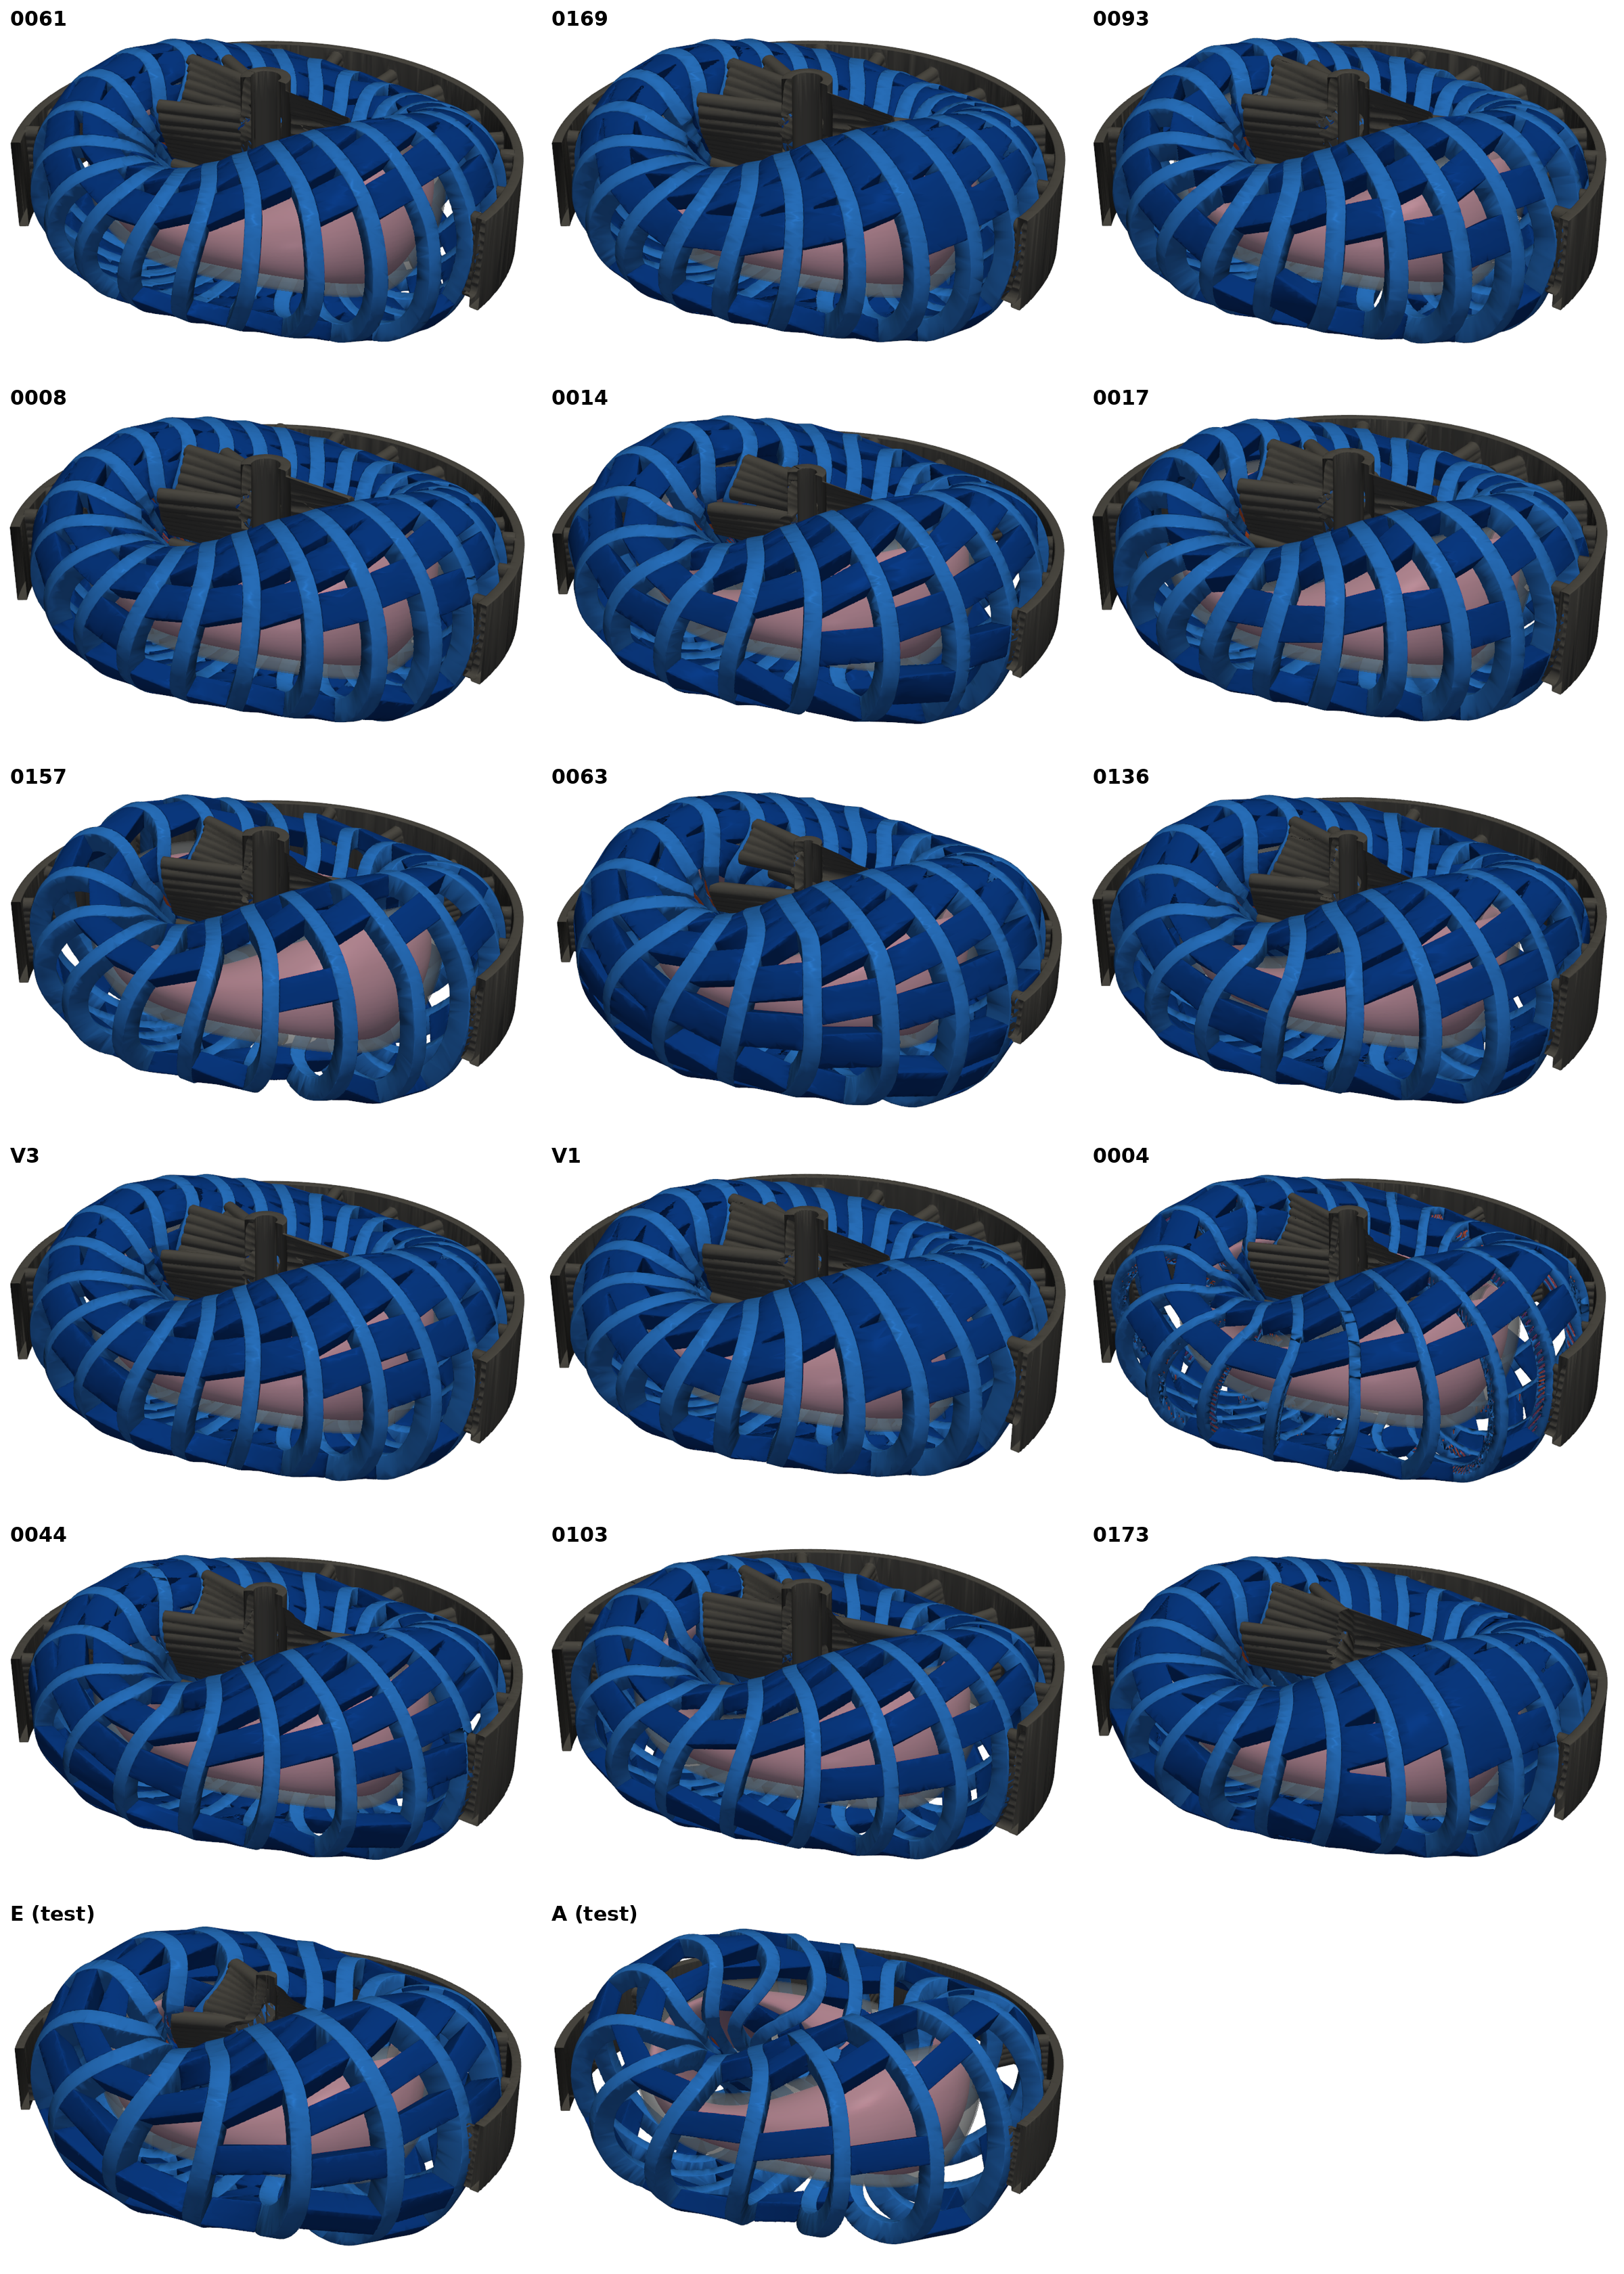
\includegraphics[width=\linewidth]{bilder/modell3d_montage.png}
\caption{Alle 3D-Modelle des Berichts (Liste 1) in der Gesamtansicht.}\end{figure}
\lesehilfe{Jedes Feld ist ein vollständiges PicoGK-Modell, beschriftet mit der Entwurfsnummer. Blau sind die
Spulengehäuse, dunkelblau die Verbinder, grau durchscheinend das Vakuumgefäß, rosa das Plasma, dunkelgrau die
schematischen Lager. Entwürfe mit 24 Spulen wirken wie ein dichter Käfig, die Tragwerksversuche A und E mit 16
Spulen offener; bei E sind die Wände sichtbar dicker.}

%======================================================================
\section{Steckbriefe der Entwürfe aus Liste~1}\label{sec:steckbriefe}
Liste~1 enthält die zulässigen Entwürfe, die fünf am knappsten verfehlten, die zwei durch die Bereinigung
herausgefallenen und die Tragwerksversuche A und E. Jeder Steckbrief zeigt Stellgrößen, Ergebnisse, die Netzstudie,
das Spannungsbild und das PicoGK-Modell im Treppenschnitt.
\lesehilfe{Spannungsbild: Draufsicht auf alle Gehäuse, Farbe von blau (\SI{0}{MPa}) über grün und gelb bis rot
(\SI{800}{MPa} und mehr). Rote Punkte an den Seiten der Gehäuse sind die Verbinderanschlüsse. Treppenschnitt: Jede
Schicht ist unter einem anderen Winkel aufgeschnitten -- von innen nach außen Plasma (rosa), Erstwand und Blanket
(gelb), Abschirmung (grün), Vakuumgefäß (grau), dann die Spulen mit ihrem orangefarbenen Wickelpaket im Querschnitt.}


\clearpage
\subsection{Entwurf 0061}\label{sb:0061}
\noindent\textbf{Urteil: }Zulässig (bereinigt), Rang 1 von 7; kleinste Reserve 30 \% (Stahl σ99).\par\smallskip
\begin{minipage}[t]{0.46\linewidth}\small\begin{tabular}[t]{@{}lr@{}}\toprule\multicolumn{2}{@{}l}{\textbf{Stellgrößen}}\\\midrule
Abstand Spule–Plasma & \num{0.204} \\
Spulen gesamt & 24 \\
Spulen je halbe Periode & \num{6} \\
Länge je Spule & \num{4.58} \\
Kraftziel & \num{0.010} \\
Wand innen & \num{0.10} \\
Seitenwand & \num{0.30} \\
Außenwand min. & \num{0.52} \\
Außenwand Zusatz & \num{0.26} \\
Verbindersteifigkeit & \num{93} \\
Verbinder je Paar & \num{10} \\
Lagerradius & \num{3.23} \\
\bottomrule\end{tabular}\end{minipage}\hfill
\begin{minipage}[t]{0.5\linewidth}\small\begin{tabular}[t]{@{}lr@{}}\toprule\multicolumn{2}{@{}l}{\textbf{Ergebnisse}}\\\midrule
$\sigma_{99}$ Stahl & \num{351} MPa \\
größtes Element & \num{725} MPa \\
$P_m$ max. / 99 \% & \num{522} / \num{379} MPa \\
$P_m+P_b$ max. & \num{938} MPa \\
Verbinder σ99 & \num{191} MPa \\
Verformung max. & \num{18} mm \\
Dehnung Wickelpaket & \num{0.17} \% \\
Strom je Spule & \num{14.7} MA \\
Feld am Leiter & \num{15.6} T \\
Auslastung / Marge & \num{30} \% / \num{24} K \\
Feldfehler $B\cdot n$ & \num{1.49} ‰ \\
Freiraum Plasma–Gehäuse & \num{1.62} m \\
Kernheizung / Fluenz & \num{10} W/m³ / 8.0e16 \\
Stahl Gehäuse + Verbinder & \num{9.5} + \num{9.9} kt \\
Verbinder gebaut & 236 \\
\bottomrule\end{tabular}\end{minipage}\par\medskip
\noindent\textit{Netzstudie ($\sigma_{99}$/max. in MPa): }doe1: 351/725; 1,5× Stationen: 556/6553; Wand 3 Zellen: 346/861.\par\smallskip
\begin{figure}[H]\centering
\begin{minipage}[t]{0.49\linewidth}\centering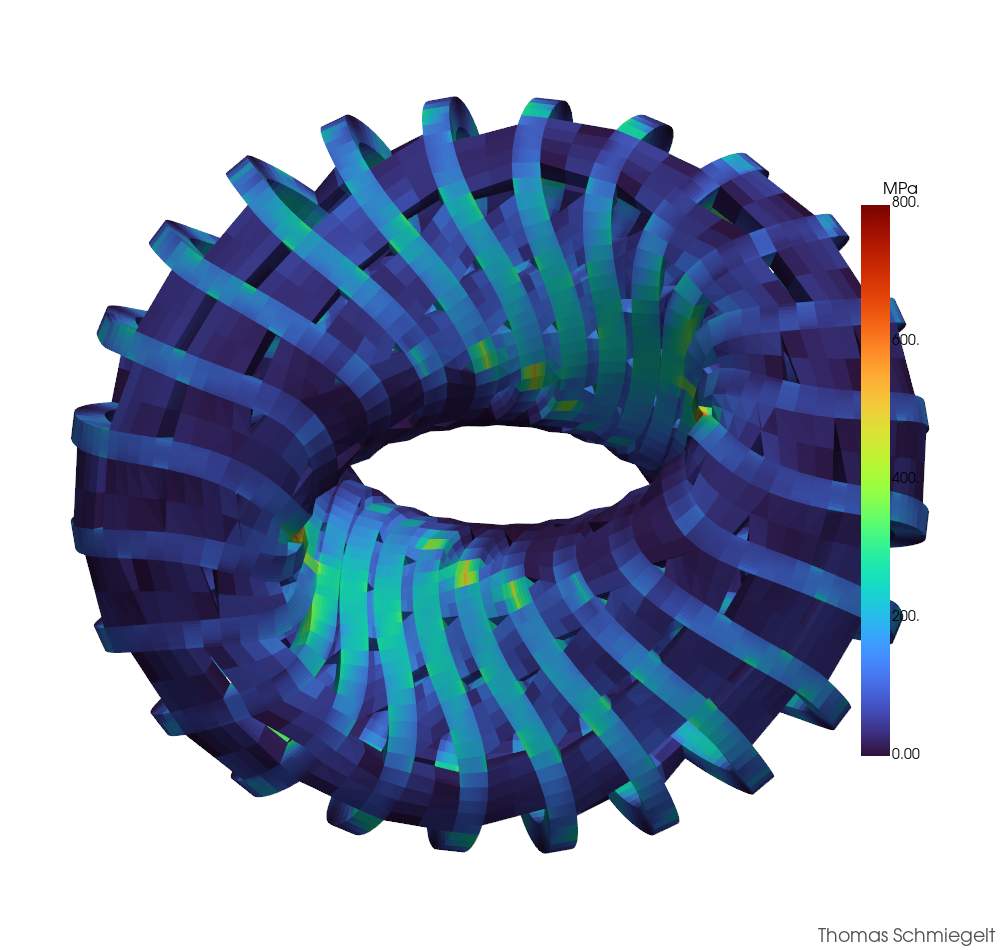
\includegraphics[width=\linewidth]{bilder/spannung_0061.png}\\\footnotesize Vergleichsspannung im Stahl (Draufsicht, 0–800 MPa)\end{minipage}\hfill
\begin{minipage}[t]{0.49\linewidth}\centering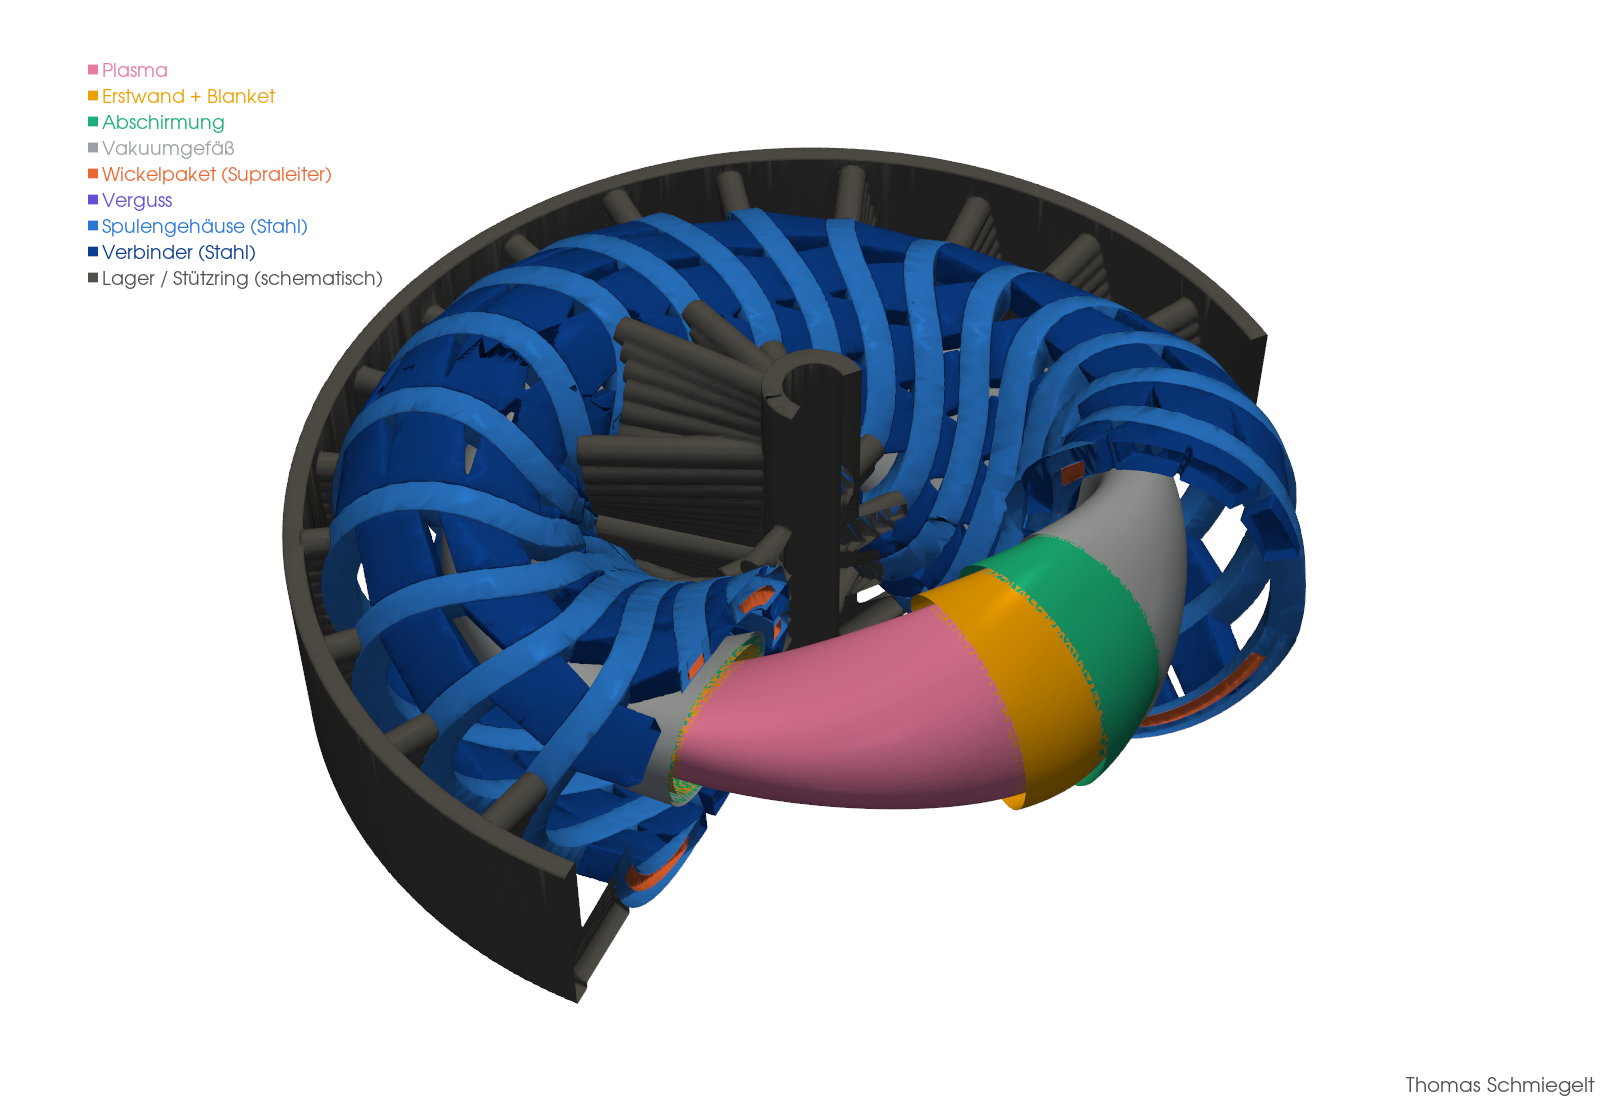
\includegraphics[width=\linewidth]{bilder/modell3d_0061_schnitt.png}\\\footnotesize PicoGK-Modell, Treppenschnitt\end{minipage}\hfill
\caption{Entwurf 0061}\end{figure}
\clearpage
\subsection{Entwurf 0169}\label{sb:0169}
\noindent\textbf{Urteil: }Zulässig (bereinigt), Rang 2 von 7; kleinste Reserve 29 \% (Platz Package).\par\smallskip
\begin{minipage}[t]{0.46\linewidth}\small\begin{tabular}[t]{@{}lr@{}}\toprule\multicolumn{2}{@{}l}{\textbf{Stellgrößen}}\\\midrule
Abstand Spule–Plasma & \num{0.197} \\
Spulen gesamt & 24 \\
Spulen je halbe Periode & \num{6} \\
Länge je Spule & \num{4.87} \\
Kraftziel & \num{0.023} \\
Wand innen & \num{0.27} \\
Seitenwand & \num{0.34} \\
Außenwand min. & \num{0.67} \\
Außenwand Zusatz & \num{0.25} \\
Verbindersteifigkeit & \num{183} \\
Verbinder je Paar & \num{13} \\
Lagerradius & \num{3.29} \\
\bottomrule\end{tabular}\end{minipage}\hfill
\begin{minipage}[t]{0.5\linewidth}\small\begin{tabular}[t]{@{}lr@{}}\toprule\multicolumn{2}{@{}l}{\textbf{Ergebnisse}}\\\midrule
$\sigma_{99}$ Stahl & \num{308} MPa \\
größtes Element & \num{717} MPa \\
$P_m$ max. / 99 \% & \num{626} / \num{333} MPa \\
$P_m+P_b$ max. & \num{817} MPa \\
Verbinder σ99 & \num{192} MPa \\
Verformung max. & \num{19} mm \\
Dehnung Wickelpaket & \num{0.15} \% \\
Strom je Spule & \num{14.7} MA \\
Feld am Leiter & \num{15.5} T \\
Auslastung / Marge & \num{30} \% / \num{24} K \\
Feldfehler $B\cdot n$ & \num{2.13} ‰ \\
Freiraum Plasma–Gehäuse & \num{1.39} m \\
Kernheizung / Fluenz & \num{103} W/m³ / 8.5e17 \\
Stahl Gehäuse + Verbinder & \num{12.8} + \num{15.2} kt \\
Verbinder gebaut & 292 \\
\bottomrule\end{tabular}\end{minipage}\par\medskip
\noindent\textit{Netzstudie ($\sigma_{99}$/max. in MPa): }doe1: 219/421; Standard: 308/717; 1,5× Stationen: 319/1262; Wand 3 Zellen: 308/794.\par\smallskip
\begin{figure}[H]\centering
\begin{minipage}[t]{0.49\linewidth}\centering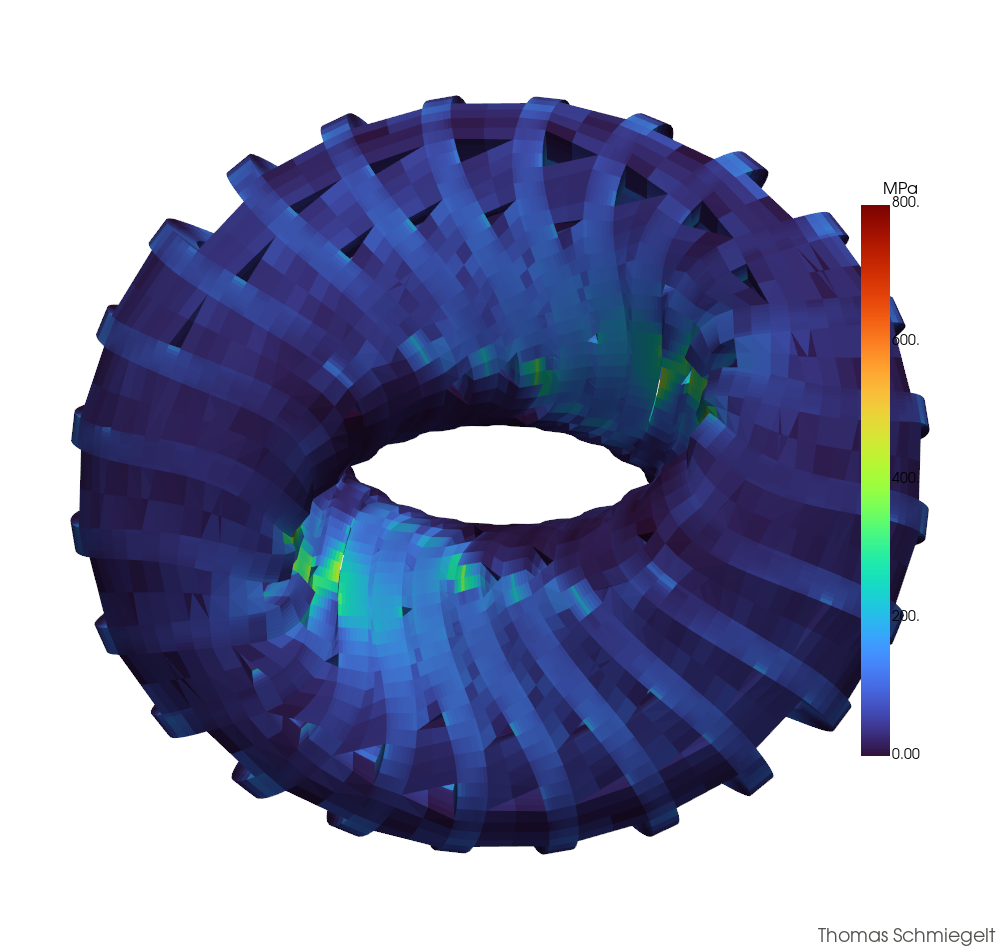
\includegraphics[width=\linewidth]{bilder/spannung_0169.png}\\\footnotesize Vergleichsspannung im Stahl (Draufsicht, 0–800 MPa)\end{minipage}\hfill
\begin{minipage}[t]{0.49\linewidth}\centering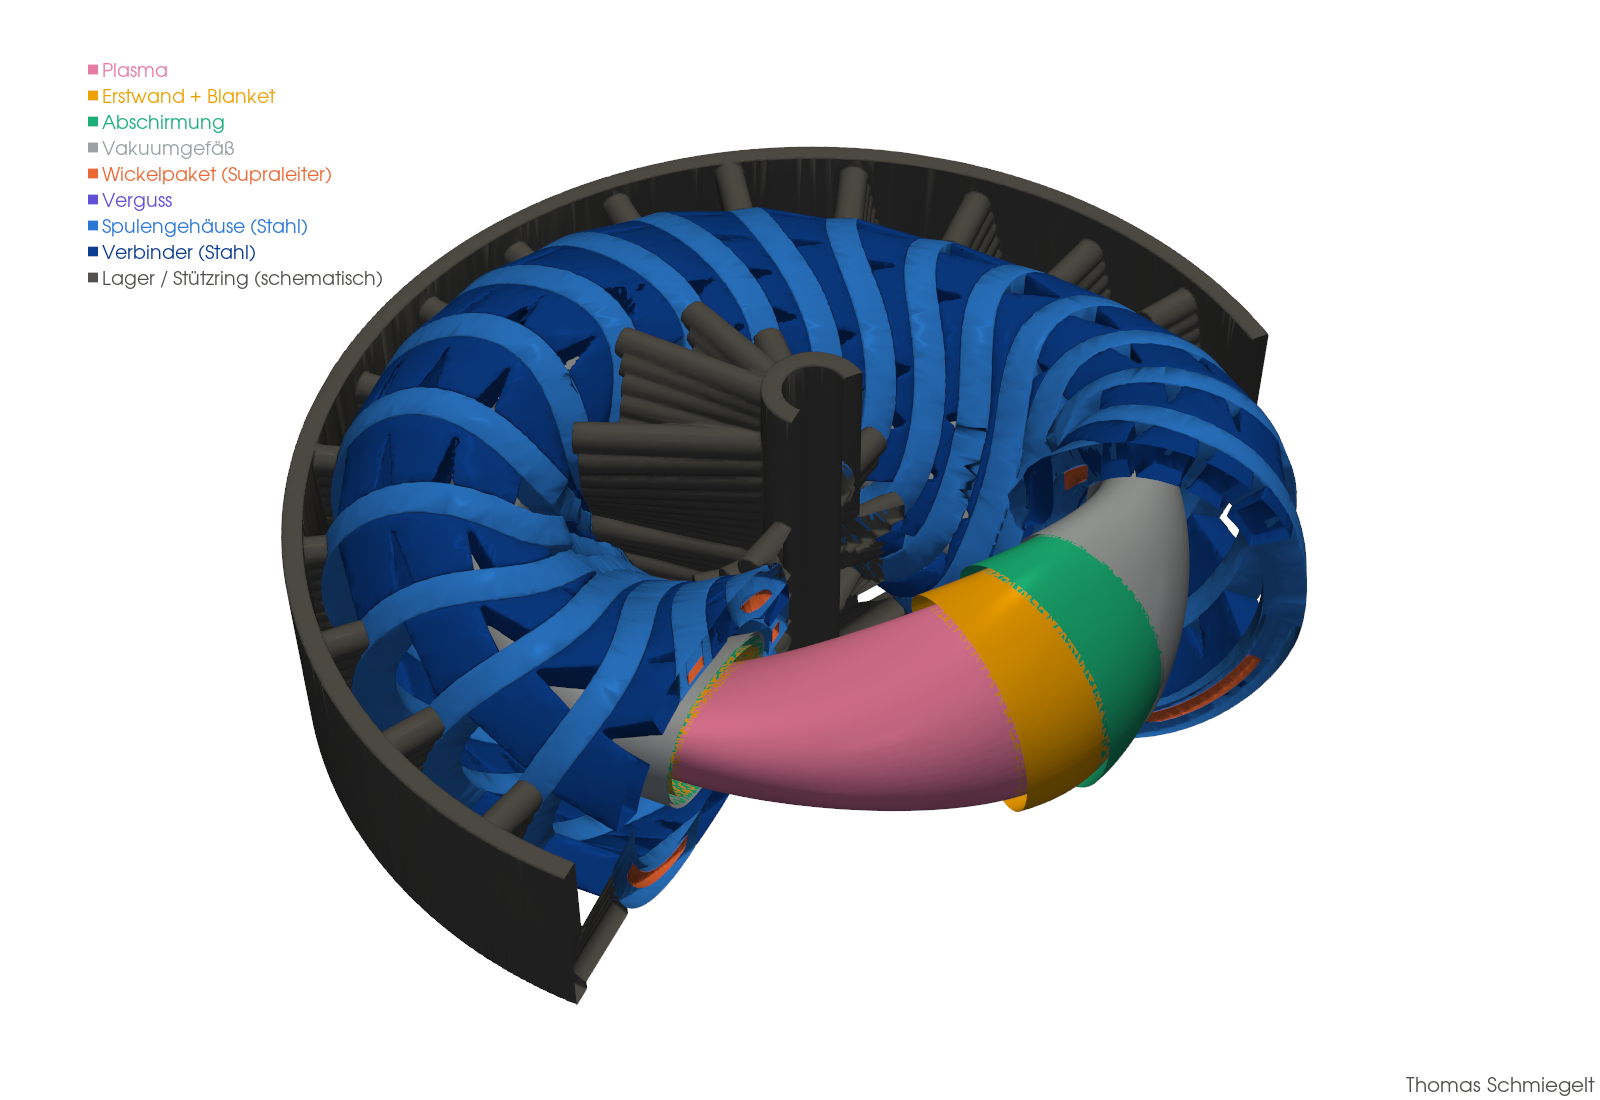
\includegraphics[width=\linewidth]{bilder/modell3d_0169_schnitt.png}\\\footnotesize PicoGK-Modell, Treppenschnitt\end{minipage}\hfill
\caption{Entwurf 0169}\end{figure}
\clearpage
\subsection{Entwurf 0093}\label{sb:0093}
\noindent\textbf{Urteil: }Zulässig (bereinigt), Rang 3 von 7; kleinste Reserve 27 \% (Platz Package).\par\smallskip
\begin{minipage}[t]{0.46\linewidth}\small\begin{tabular}[t]{@{}lr@{}}\toprule\multicolumn{2}{@{}l}{\textbf{Stellgrößen}}\\\midrule
Abstand Spule–Plasma & \num{0.206} \\
Spulen gesamt & 24 \\
Spulen je halbe Periode & \num{6} \\
Länge je Spule & \num{4.14} \\
Kraftziel & \num{0.010} \\
Wand innen & \num{0.38} \\
Seitenwand & \num{0.38} \\
Außenwand min. & \num{0.73} \\
Außenwand Zusatz & \num{0.38} \\
Verbindersteifigkeit & \num{64} \\
Verbinder je Paar & \num{8} \\
Lagerradius & \num{3.49} \\
\bottomrule\end{tabular}\end{minipage}\hfill
\begin{minipage}[t]{0.5\linewidth}\small\begin{tabular}[t]{@{}lr@{}}\toprule\multicolumn{2}{@{}l}{\textbf{Ergebnisse}}\\\midrule
$\sigma_{99}$ Stahl & \num{283} MPa \\
größtes Element & \num{1190} MPa \\
$P_m$ max. / 99 \% & \num{1147} / \num{340} MPa \\
$P_m+P_b$ max. & \num{1233} MPa \\
Verbinder σ99 & \num{154} MPa \\
Verformung max. & \num{20} mm \\
Dehnung Wickelpaket & \num{0.16} \% \\
Strom je Spule & \num{14.7} MA \\
Feld am Leiter & \num{15.7} T \\
Auslastung / Marge & \num{30} \% / \num{24} K \\
Feldfehler $B\cdot n$ & \num{1.45} ‰ \\
Freiraum Plasma–Gehäuse & \num{1.37} m \\
Kernheizung / Fluenz & \num{117} W/m³ / 9.8e17 \\
Stahl Gehäuse + Verbinder & \num{16.5} + \num{11.6} kt \\
Verbinder gebaut & 190 \\
\bottomrule\end{tabular}\end{minipage}\par\medskip
\noindent\textit{Netzstudie ($\sigma_{99}$/max. in MPa): }doe1: 283/1190; 1,5× Stationen: 410/2343; Wand 3 Zellen: 280/1432.\par\smallskip
\begin{figure}[H]\centering
\begin{minipage}[t]{0.49\linewidth}\centering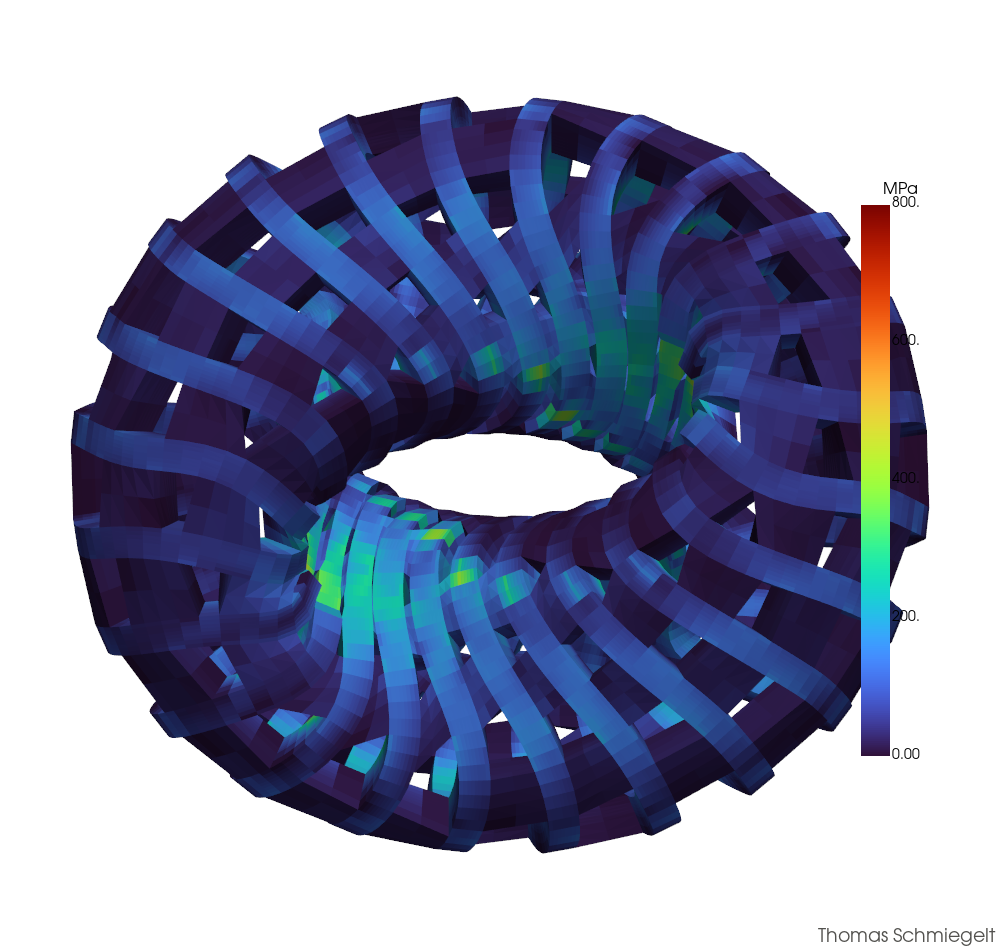
\includegraphics[width=\linewidth]{bilder/spannung_0093.png}\\\footnotesize Vergleichsspannung im Stahl (Draufsicht, 0–800 MPa)\end{minipage}\hfill
\begin{minipage}[t]{0.49\linewidth}\centering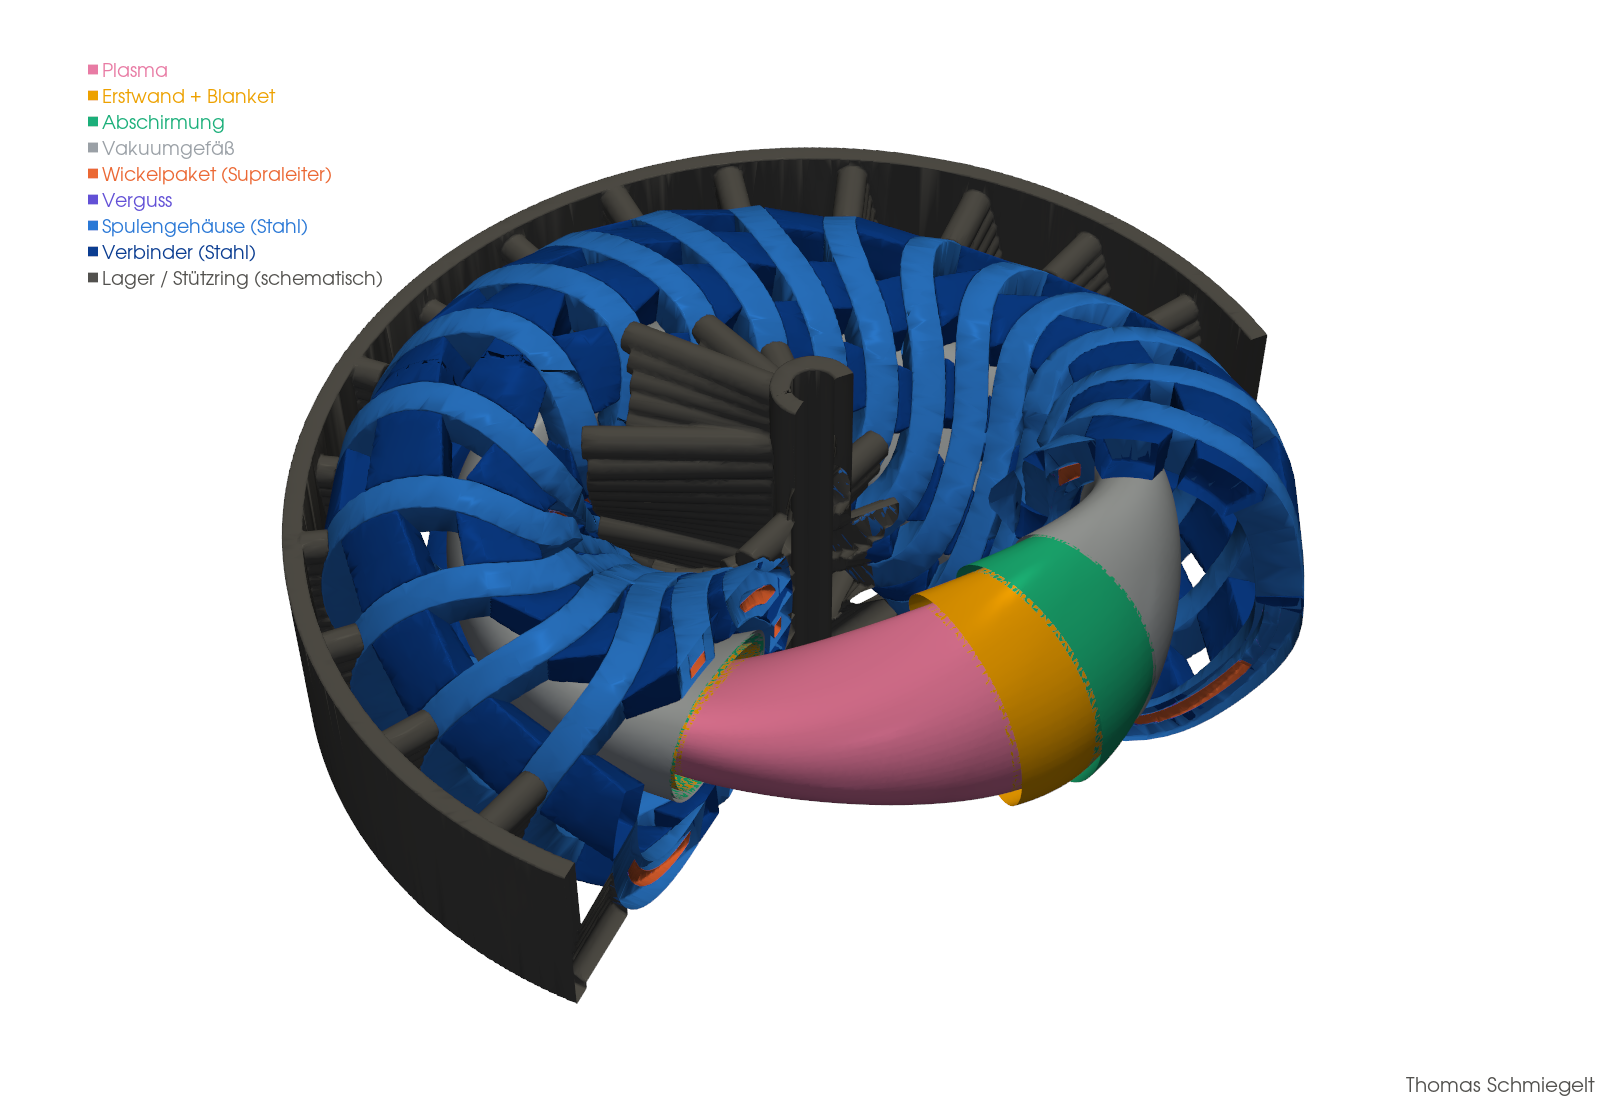
\includegraphics[width=\linewidth]{bilder/modell3d_0093_schnitt.png}\\\footnotesize PicoGK-Modell, Treppenschnitt\end{minipage}\hfill
\caption{Entwurf 0093}\end{figure}
\clearpage
\subsection{Entwurf 0008}\label{sb:0008}
\noindent\textbf{Urteil: }Zulässig (bereinigt), Rang 4 von 7; kleinste Reserve 27 \% (Feldfehler B·n).\par\smallskip
\begin{minipage}[t]{0.46\linewidth}\small\begin{tabular}[t]{@{}lr@{}}\toprule\multicolumn{2}{@{}l}{\textbf{Stellgrößen}}\\\midrule
Abstand Spule–Plasma & \num{0.211} \\
Spulen gesamt & 24 \\
Spulen je halbe Periode & \num{6} \\
Länge je Spule & \num{3.66} \\
Kraftziel & \num{0.030} \\
Wand innen & \num{0.32} \\
Seitenwand & \num{0.31} \\
Außenwand min. & \num{0.72} \\
Außenwand Zusatz & \num{0.17} \\
Verbindersteifigkeit & \num{142} \\
Verbinder je Paar & \num{11} \\
Lagerradius & \num{2.80} \\
\bottomrule\end{tabular}\end{minipage}\hfill
\begin{minipage}[t]{0.5\linewidth}\small\begin{tabular}[t]{@{}lr@{}}\toprule\multicolumn{2}{@{}l}{\textbf{Ergebnisse}}\\\midrule
$\sigma_{99}$ Stahl & \num{305} MPa \\
größtes Element & \num{1695} MPa \\
$P_m$ max. / 99 \% & \num{1687} / \num{344} MPa \\
$P_m+P_b$ max. & \num{1704} MPa \\
Verbinder σ99 & \num{187} MPa \\
Verformung max. & \num{19} mm \\
Dehnung Wickelpaket & \num{0.17} \% \\
Strom je Spule & \num{14.7} MA \\
Feld am Leiter & \num{15.7} T \\
Auslastung / Marge & \num{30} \% / \num{24} K \\
Feldfehler $B\cdot n$ & \num{2.20} ‰ \\
Freiraum Plasma–Gehäuse & \num{1.48} m \\
Kernheizung / Fluenz & \num{40} W/m³ / 3.3e17 \\
Stahl Gehäuse + Verbinder & \num{12.2} + \num{13.7} kt \\
Verbinder gebaut & 252 \\
\bottomrule\end{tabular}\end{minipage}\par\medskip
\noindent\textit{Netzstudie ($\sigma_{99}$/max. in MPa): }doe1: 305/1695; 1,5× Stationen: 407/3250; Wand 3 Zellen: 306/1931.\par\smallskip
\begin{figure}[H]\centering
\begin{minipage}[t]{0.49\linewidth}\centering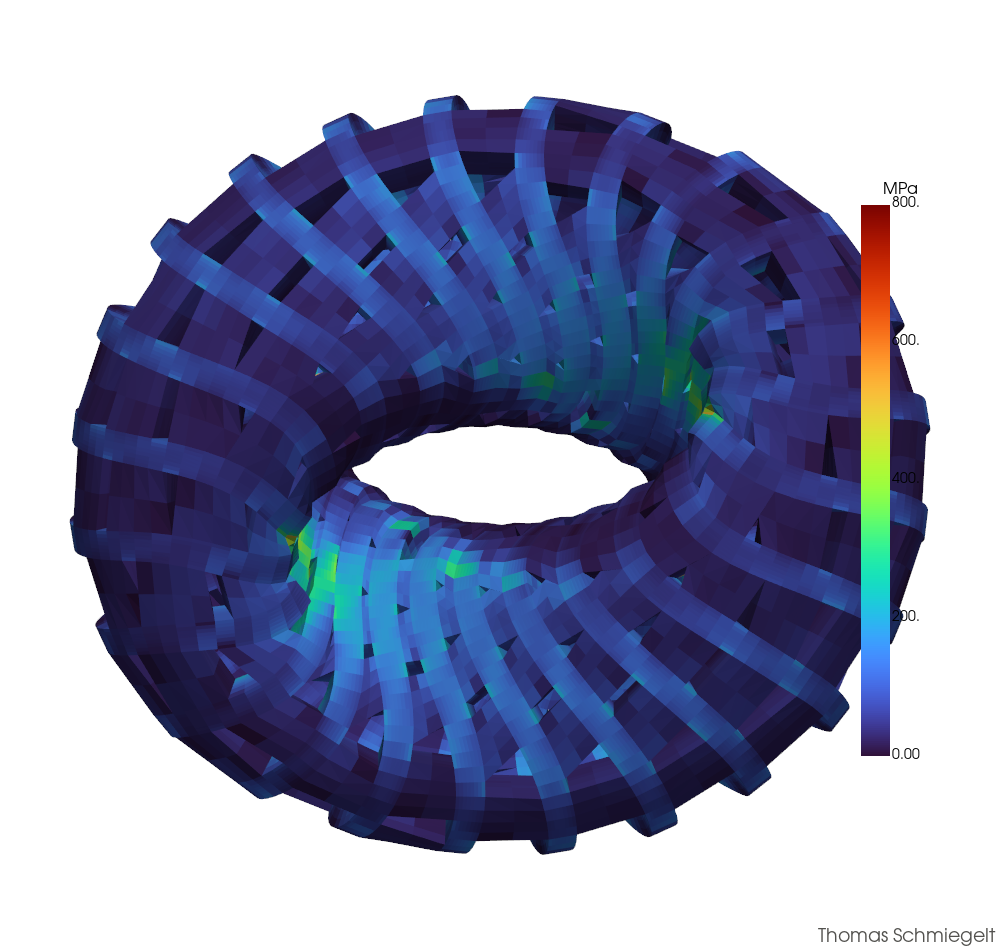
\includegraphics[width=\linewidth]{bilder/spannung_0008.png}\\\footnotesize Vergleichsspannung im Stahl (Draufsicht, 0–800 MPa)\end{minipage}\hfill
\begin{minipage}[t]{0.49\linewidth}\centering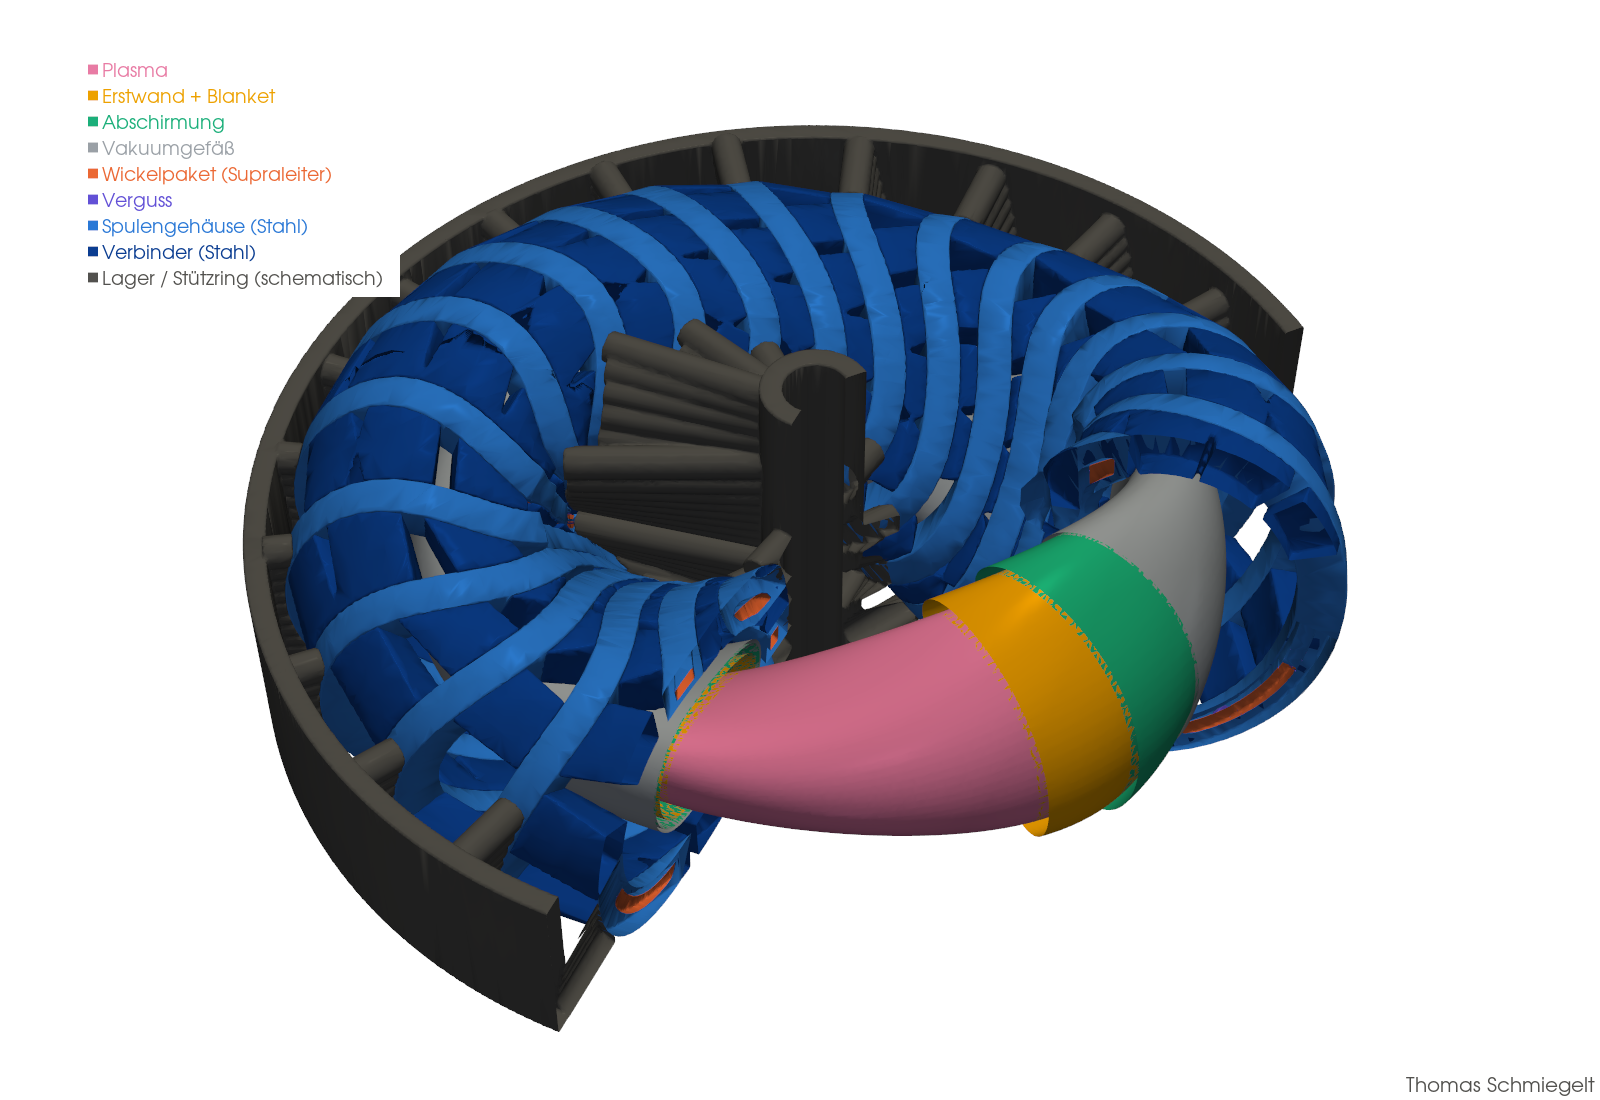
\includegraphics[width=\linewidth]{bilder/modell3d_0008_schnitt.png}\\\footnotesize PicoGK-Modell, Treppenschnitt\end{minipage}\hfill
\caption{Entwurf 0008}\end{figure}
\clearpage
\subsection{Entwurf 0014}\label{sb:0014}
\noindent\textbf{Urteil: }Zulässig (bereinigt), Rang 5 von 7; kleinste Reserve 25 \% (Stahl σ99).\par\smallskip
\begin{minipage}[t]{0.46\linewidth}\small\begin{tabular}[t]{@{}lr@{}}\toprule\multicolumn{2}{@{}l}{\textbf{Stellgrößen}}\\\midrule
Abstand Spule–Plasma & \num{0.233} \\
Spulen gesamt & 20 \\
Spulen je halbe Periode & \num{5} \\
Länge je Spule & \num{4.34} \\
Kraftziel & \num{0.025} \\
Wand innen & \num{0.35} \\
Seitenwand & \num{0.32} \\
Außenwand min. & \num{0.63} \\
Außenwand Zusatz & \num{0.29} \\
Verbindersteifigkeit & \num{196} \\
Verbinder je Paar & \num{11} \\
Lagerradius & \num{2.04} \\
\bottomrule\end{tabular}\end{minipage}\hfill
\begin{minipage}[t]{0.5\linewidth}\small\begin{tabular}[t]{@{}lr@{}}\toprule\multicolumn{2}{@{}l}{\textbf{Ergebnisse}}\\\midrule
$\sigma_{99}$ Stahl & \num{377} MPa \\
größtes Element & \num{1419} MPa \\
$P_m$ max. / 99 \% & \num{1369} / \num{459} MPa \\
$P_m+P_b$ max. & \num{1491} MPa \\
Verbinder σ99 & \num{243} MPa \\
Verformung max. & \num{18} mm \\
Dehnung Wickelpaket & \num{0.21} \% \\
Strom je Spule & \num{17.7} MA \\
Feld am Leiter & \num{16.9} T \\
Auslastung / Marge & \num{32} \% / \num{23} K \\
Feldfehler $B\cdot n$ & \num{2.21} ‰ \\
Freiraum Plasma–Gehäuse & \num{1.65} m \\
Kernheizung / Fluenz & \num{8} W/m³ / 6.5e16 \\
Stahl Gehäuse + Verbinder & \num{12.5} + \num{15.5} kt \\
Verbinder gebaut & 212 \\
\bottomrule\end{tabular}\end{minipage}\par\medskip
\noindent\textit{Netzstudie ($\sigma_{99}$/max. in MPa): }doe1: 377/1419; 1,5× Stationen: 549/3814; Wand 3 Zellen: 375/1639.\par\smallskip
\begin{figure}[H]\centering
\begin{minipage}[t]{0.49\linewidth}\centering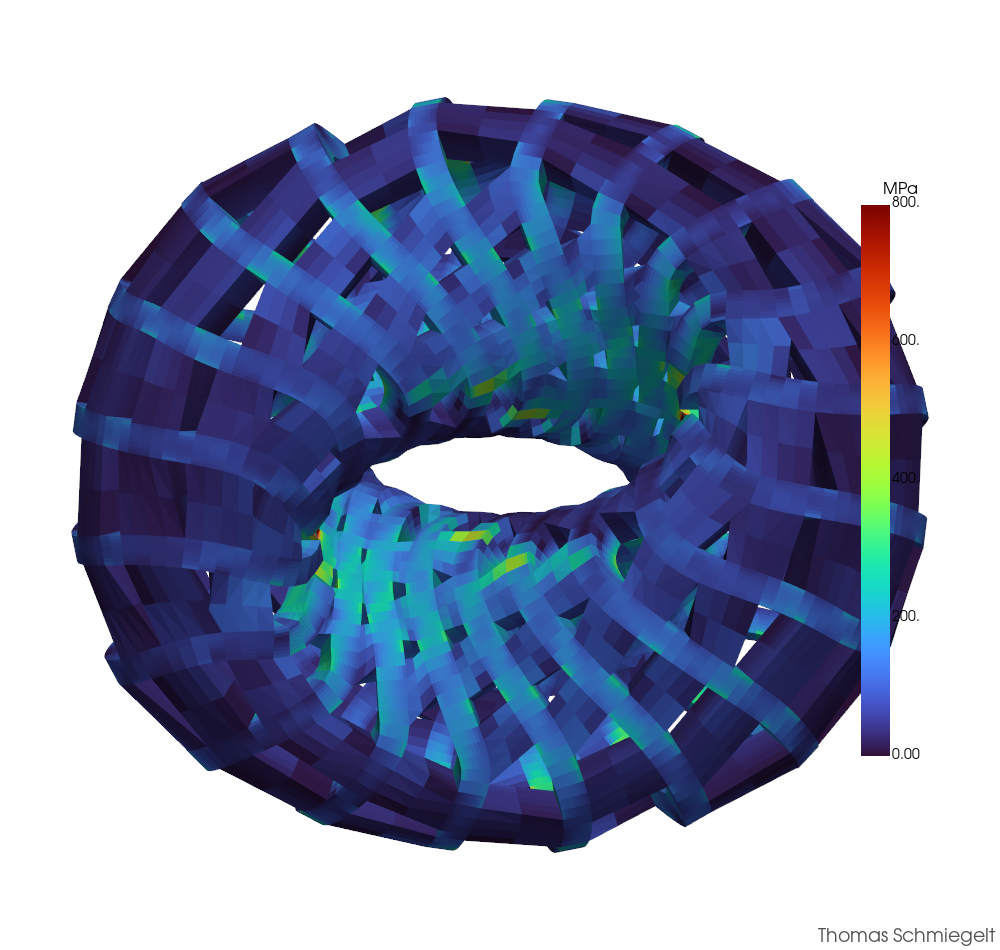
\includegraphics[width=\linewidth]{bilder/spannung_0014.png}\\\footnotesize Vergleichsspannung im Stahl (Draufsicht, 0–800 MPa)\end{minipage}\hfill
\begin{minipage}[t]{0.49\linewidth}\centering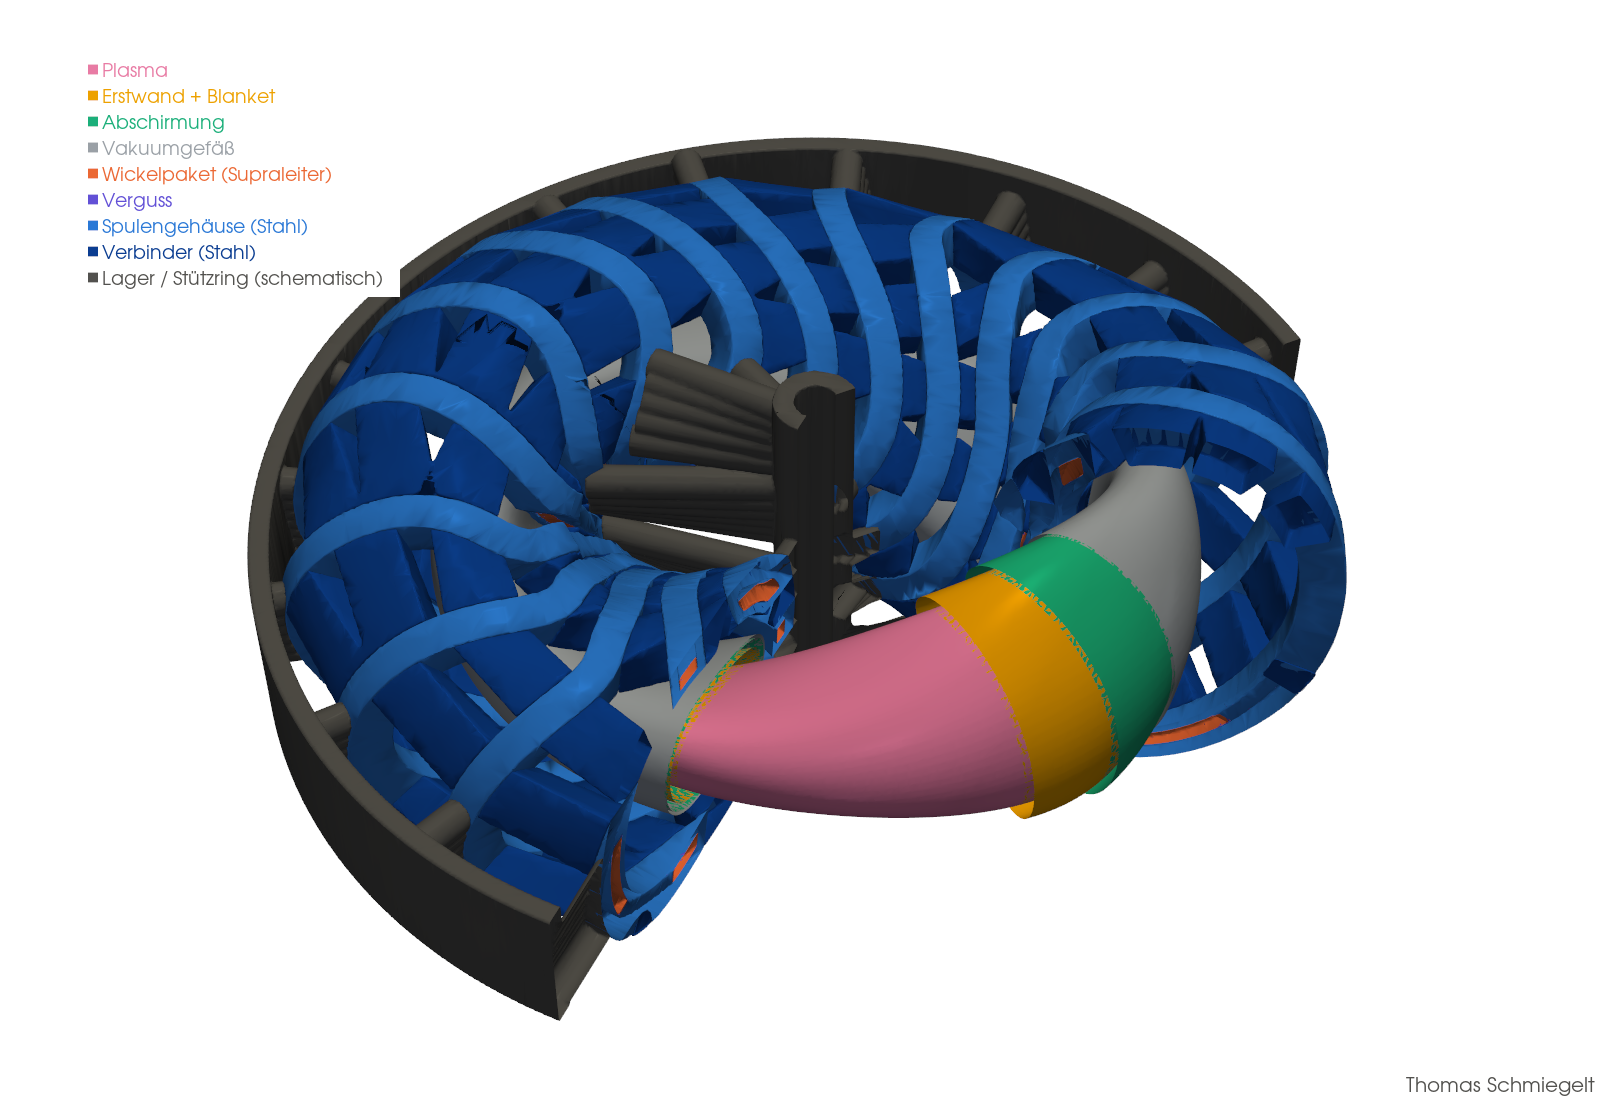
\includegraphics[width=\linewidth]{bilder/modell3d_0014_schnitt.png}\\\footnotesize PicoGK-Modell, Treppenschnitt\end{minipage}\hfill
\caption{Entwurf 0014}\end{figure}
\clearpage
\subsection{Entwurf 0017}\label{sb:0017}
\noindent\textbf{Urteil: }Zulässig (bereinigt), Rang 6 von 7; kleinste Reserve 20 \% (Platz Package).\par\smallskip
\begin{minipage}[t]{0.46\linewidth}\small\begin{tabular}[t]{@{}lr@{}}\toprule\multicolumn{2}{@{}l}{\textbf{Stellgrößen}}\\\midrule
Abstand Spule–Plasma & \num{0.220} \\
Spulen gesamt & 24 \\
Spulen je halbe Periode & \num{6} \\
Länge je Spule & \num{3.77} \\
Kraftziel & \num{0.019} \\
Wand innen & \num{0.60} \\
Seitenwand & \num{0.37} \\
Außenwand min. & \num{0.43} \\
Außenwand Zusatz & \num{0.32} \\
Verbindersteifigkeit & \num{29} \\
Verbinder je Paar & \num{7} \\
Lagerradius & \num{3.47} \\
\bottomrule\end{tabular}\end{minipage}\hfill
\begin{minipage}[t]{0.5\linewidth}\small\begin{tabular}[t]{@{}lr@{}}\toprule\multicolumn{2}{@{}l}{\textbf{Ergebnisse}}\\\midrule
$\sigma_{99}$ Stahl & \num{389} MPa \\
größtes Element & \num{1721} MPa \\
$P_m$ max. / 99 \% & \num{1631} / \num{448} MPa \\
$P_m+P_b$ max. & \num{1813} MPa \\
Verbinder σ99 & \num{131} MPa \\
Verformung max. & \num{31} mm \\
Dehnung Wickelpaket & \num{0.20} \% \\
Strom je Spule & \num{14.7} MA \\
Feld am Leiter & \num{16.0} T \\
Auslastung / Marge & \num{30} \% / \num{24} K \\
Feldfehler $B\cdot n$ & \num{1.66} ‰ \\
Freiraum Plasma–Gehäuse & \num{1.30} m \\
Kernheizung / Fluenz & \num{245} W/m³ / 2.0e18 \\
Stahl Gehäuse + Verbinder & \num{13.9} + \num{8.7} kt \\
Verbinder gebaut & 162 \\
\bottomrule\end{tabular}\end{minipage}\par\medskip
\begin{figure}[H]\centering
\begin{minipage}[t]{0.49\linewidth}\centering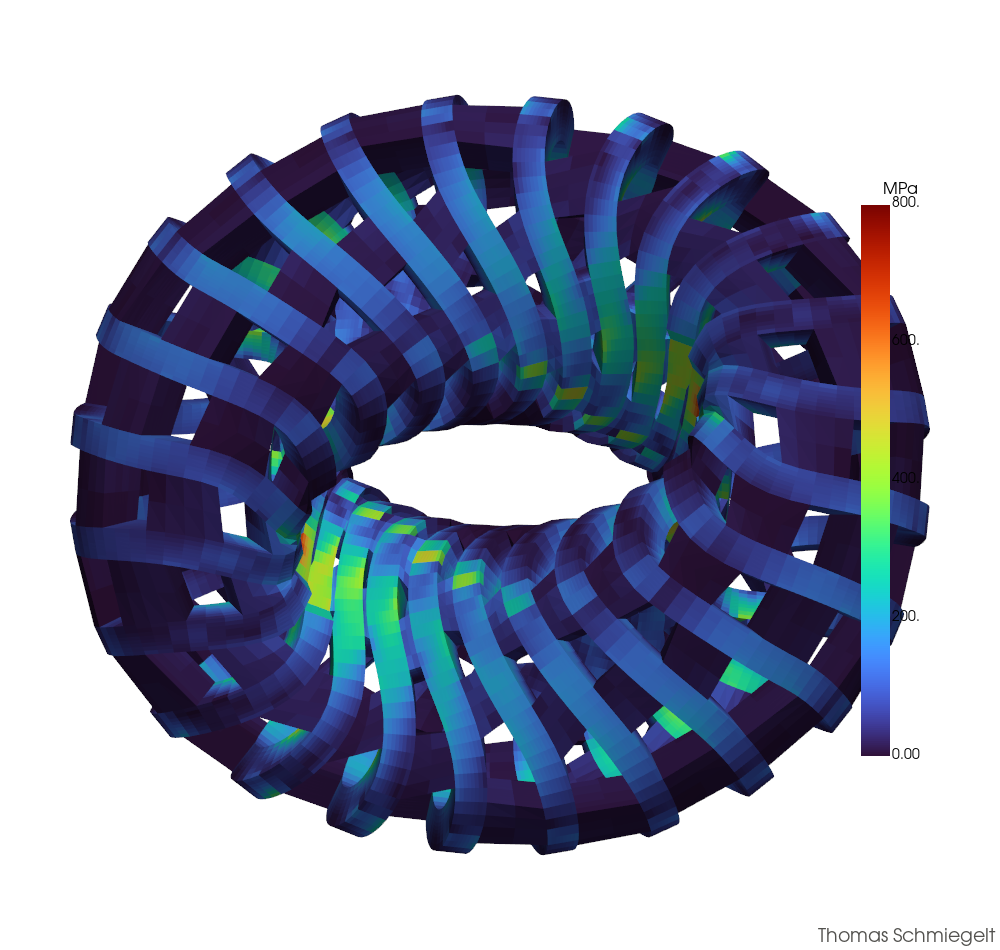
\includegraphics[width=\linewidth]{bilder/spannung_0017.png}\\\footnotesize Vergleichsspannung im Stahl (Draufsicht, 0–800 MPa)\end{minipage}\hfill
\begin{minipage}[t]{0.49\linewidth}\centering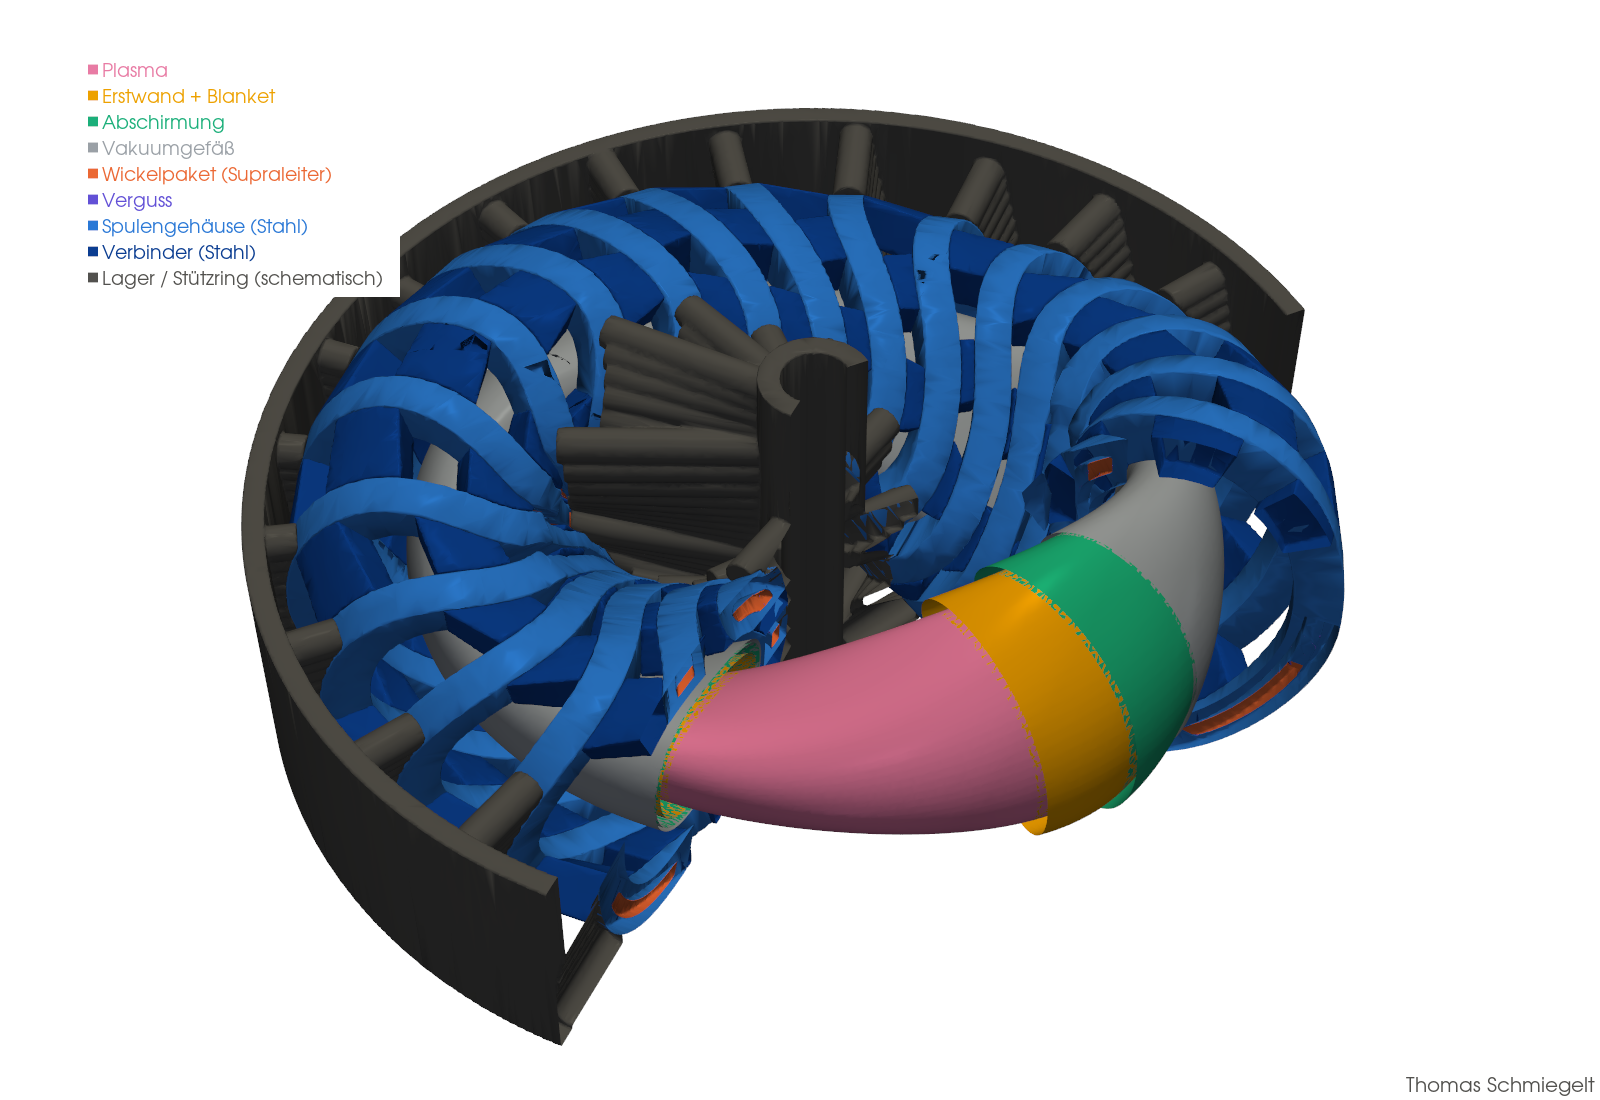
\includegraphics[width=\linewidth]{bilder/modell3d_0017_schnitt.png}\\\footnotesize PicoGK-Modell, Treppenschnitt\end{minipage}\hfill
\caption{Entwurf 0017}\end{figure}
\clearpage
\subsection{Entwurf 0157}\label{sb:0157}
\noindent\textbf{Urteil: }Zulässig (bereinigt), Rang 7 von 7; kleinste Reserve 2 \% (Stahl σ99).\par\smallskip
\begin{minipage}[t]{0.46\linewidth}\small\begin{tabular}[t]{@{}lr@{}}\toprule\multicolumn{2}{@{}l}{\textbf{Stellgrößen}}\\\midrule
Abstand Spule–Plasma & \num{0.218} \\
Spulen gesamt & 20 \\
Spulen je halbe Periode & \num{5} \\
Länge je Spule & \num{4.09} \\
Kraftziel & \num{0.020} \\
Wand innen & \num{0.49} \\
Seitenwand & \num{0.25} \\
Außenwand min. & \num{0.58} \\
Außenwand Zusatz & \num{0.02} \\
Verbindersteifigkeit & \num{158} \\
Verbinder je Paar & \num{6} \\
Lagerradius & \num{3.06} \\
\bottomrule\end{tabular}\end{minipage}\hfill
\begin{minipage}[t]{0.5\linewidth}\small\begin{tabular}[t]{@{}lr@{}}\toprule\multicolumn{2}{@{}l}{\textbf{Ergebnisse}}\\\midrule
$\sigma_{99}$ Stahl & \num{492} MPa \\
größtes Element & \num{1658} MPa \\
$P_m$ max. / 99 \% & \num{1405} / \num{519} MPa \\
$P_m+P_b$ max. & \num{1920} MPa \\
Verbinder σ99 & \num{335} MPa \\
Verformung max. & \num{34} mm \\
Dehnung Wickelpaket & \num{0.22} \% \\
Strom je Spule & \num{17.7} MA \\
Feld am Leiter & \num{16.5} T \\
Auslastung / Marge & \num{31} \% / \num{23} K \\
Feldfehler $B\cdot n$ & \num{2.37} ‰ \\
Freiraum Plasma–Gehäuse & \num{1.35} m \\
Kernheizung / Fluenz & \num{142} W/m³ / 1.2e18 \\
Stahl Gehäuse + Verbinder & \num{10.1} + \num{7.5} kt \\
Verbinder gebaut & 118 \\
\bottomrule\end{tabular}\end{minipage}\par\medskip
\begin{figure}[H]\centering
\begin{minipage}[t]{0.49\linewidth}\centering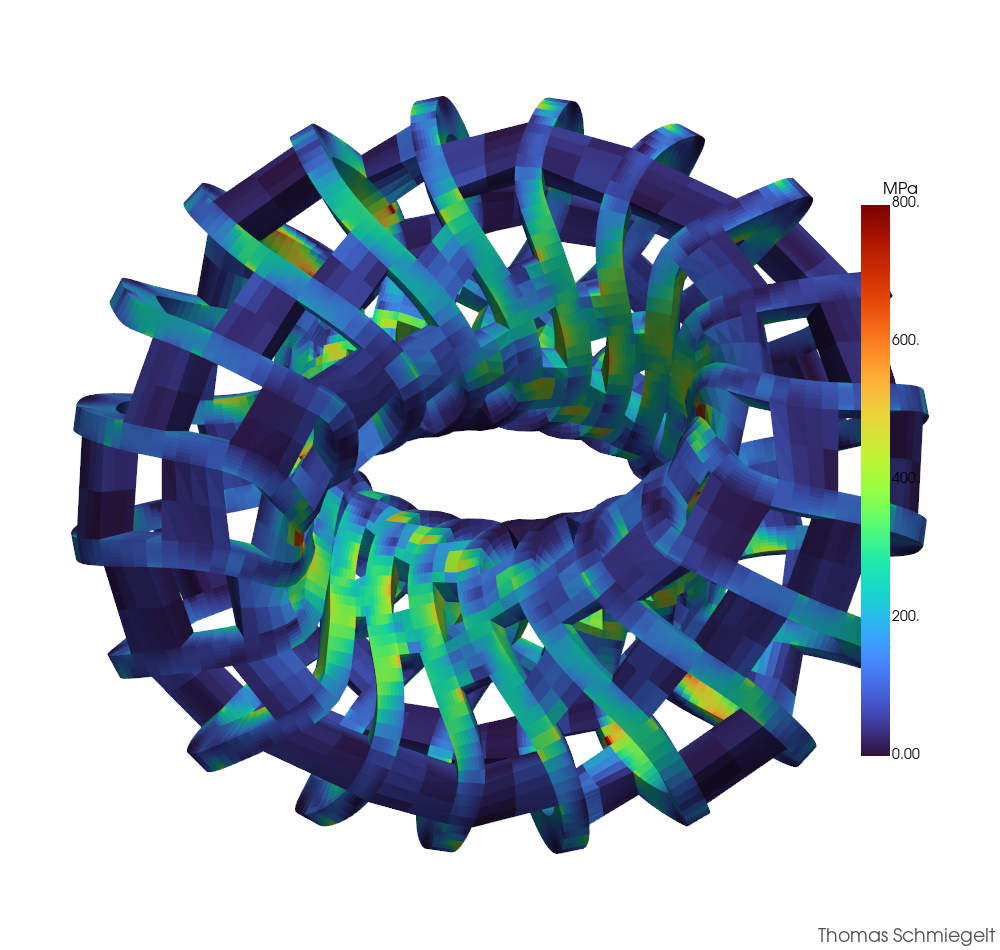
\includegraphics[width=\linewidth]{bilder/spannung_0157.png}\\\footnotesize Vergleichsspannung im Stahl (Draufsicht, 0–800 MPa)\end{minipage}\hfill
\begin{minipage}[t]{0.49\linewidth}\centering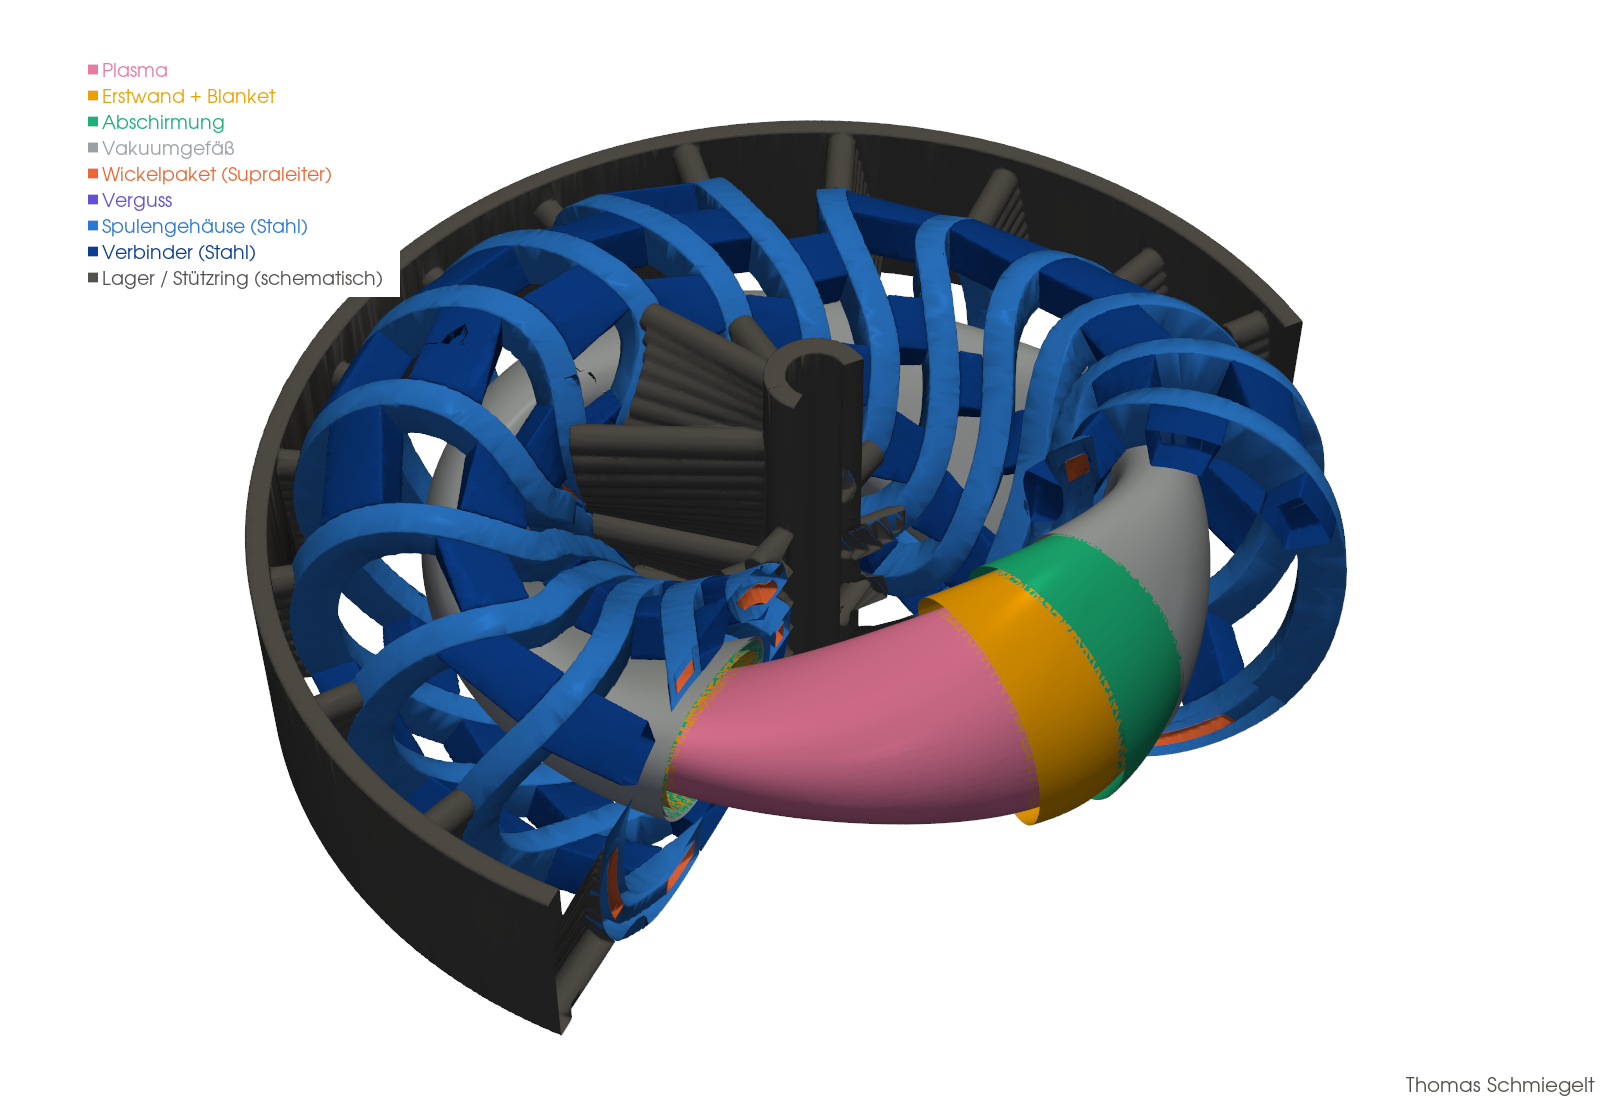
\includegraphics[width=\linewidth]{bilder/modell3d_0157_schnitt.png}\\\footnotesize PicoGK-Modell, Treppenschnitt\end{minipage}\hfill
\caption{Entwurf 0157}\end{figure}
\clearpage
\subsection{Entwurf 0063}\label{sb:0063}
\noindent\textbf{Urteil: }In doe1 zulässig, mit Standardnetz nicht mehr: Engpass Dehnung Wickelpaket (Reserve -24 \%).\par\smallskip
\begin{minipage}[t]{0.46\linewidth}\small\begin{tabular}[t]{@{}lr@{}}\toprule\multicolumn{2}{@{}l}{\textbf{Stellgrößen}}\\\midrule
Abstand Spule–Plasma & \num{0.177} \\
Spulen gesamt & 20 \\
Spulen je halbe Periode & \num{5} \\
Länge je Spule & \num{4.45} \\
Kraftziel & \num{0.000} \\
Wand innen & \num{0.59} \\
Seitenwand & \num{0.35} \\
Außenwand min. & \num{0.69} \\
Außenwand Zusatz & \num{0.44} \\
Verbindersteifigkeit & \num{43} \\
Verbinder je Paar & \num{14} \\
Lagerradius & \num{1.71} \\
\bottomrule\end{tabular}\end{minipage}\hfill
\begin{minipage}[t]{0.5\linewidth}\small\begin{tabular}[t]{@{}lr@{}}\toprule\multicolumn{2}{@{}l}{\textbf{Ergebnisse}}\\\midrule
$\sigma_{99}$ Stahl & \num{595} MPa \\
größtes Element & \num{4265} MPa \\
$P_m$ max. / 99 \% & \num{4261} / \num{942} MPa \\
$P_m+P_b$ max. & \num{4270} MPa \\
Verbinder σ99 & \num{200} MPa \\
Verformung max. & \num{81} mm \\
Dehnung Wickelpaket & \num{0.37} \% \\
Strom je Spule & \num{17.7} MA \\
Feld am Leiter & \num{17.5} T \\
Auslastung / Marge & \num{33} \% / \num{22} K \\
Feldfehler $B\cdot n$ & \num{0.75} ‰ \\
Freiraum Plasma–Gehäuse & \num{1.53} m \\
Kernheizung / Fluenz & \num{24} W/m³ / 2.0e17 \\
Stahl Gehäuse + Verbinder & \num{16.7} + \num{24.2} kt \\
Verbinder gebaut & 252 \\
\bottomrule\end{tabular}\end{minipage}\par\medskip
\noindent\textit{Netzstudie ($\sigma_{99}$/max. in MPa): }doe1: 369/2016; Standard: 595/4265.\par\smallskip
\begin{figure}[H]\centering
\begin{minipage}[t]{0.49\linewidth}\centering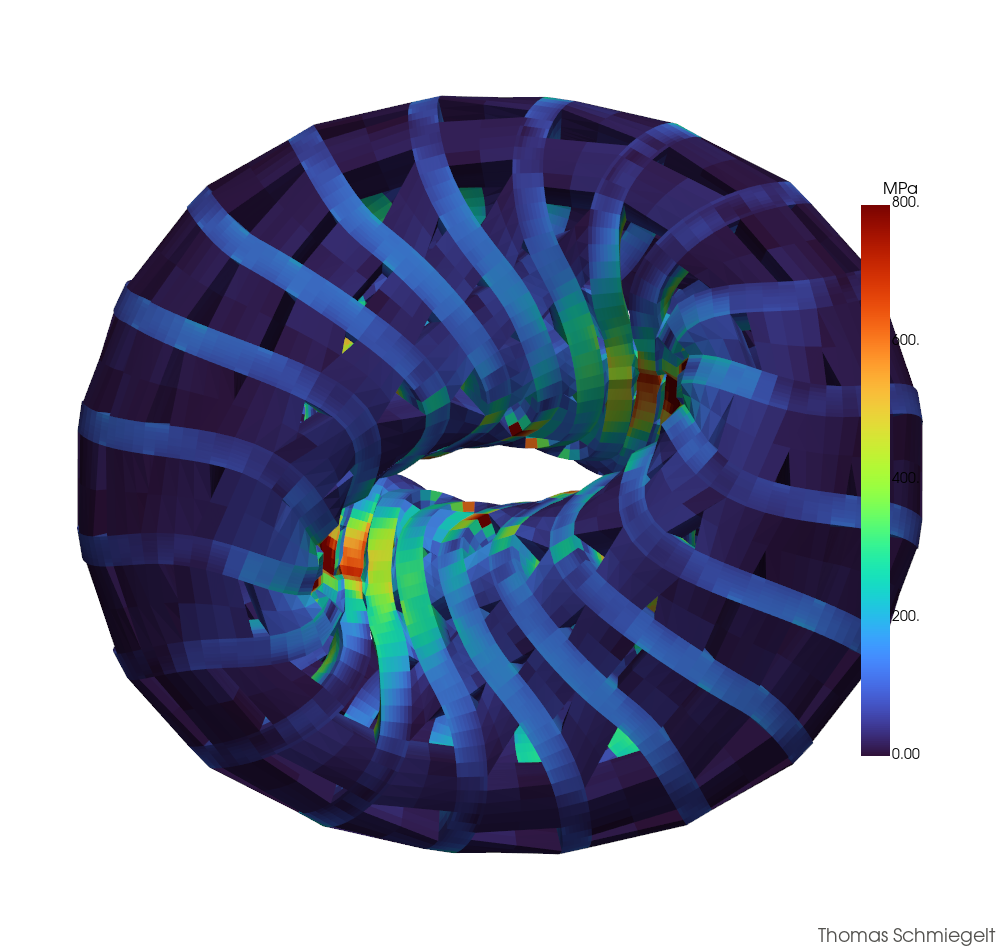
\includegraphics[width=\linewidth]{bilder/spannung_0063.png}\\\footnotesize Vergleichsspannung im Stahl (Draufsicht, 0–800 MPa)\end{minipage}\hfill
\begin{minipage}[t]{0.49\linewidth}\centering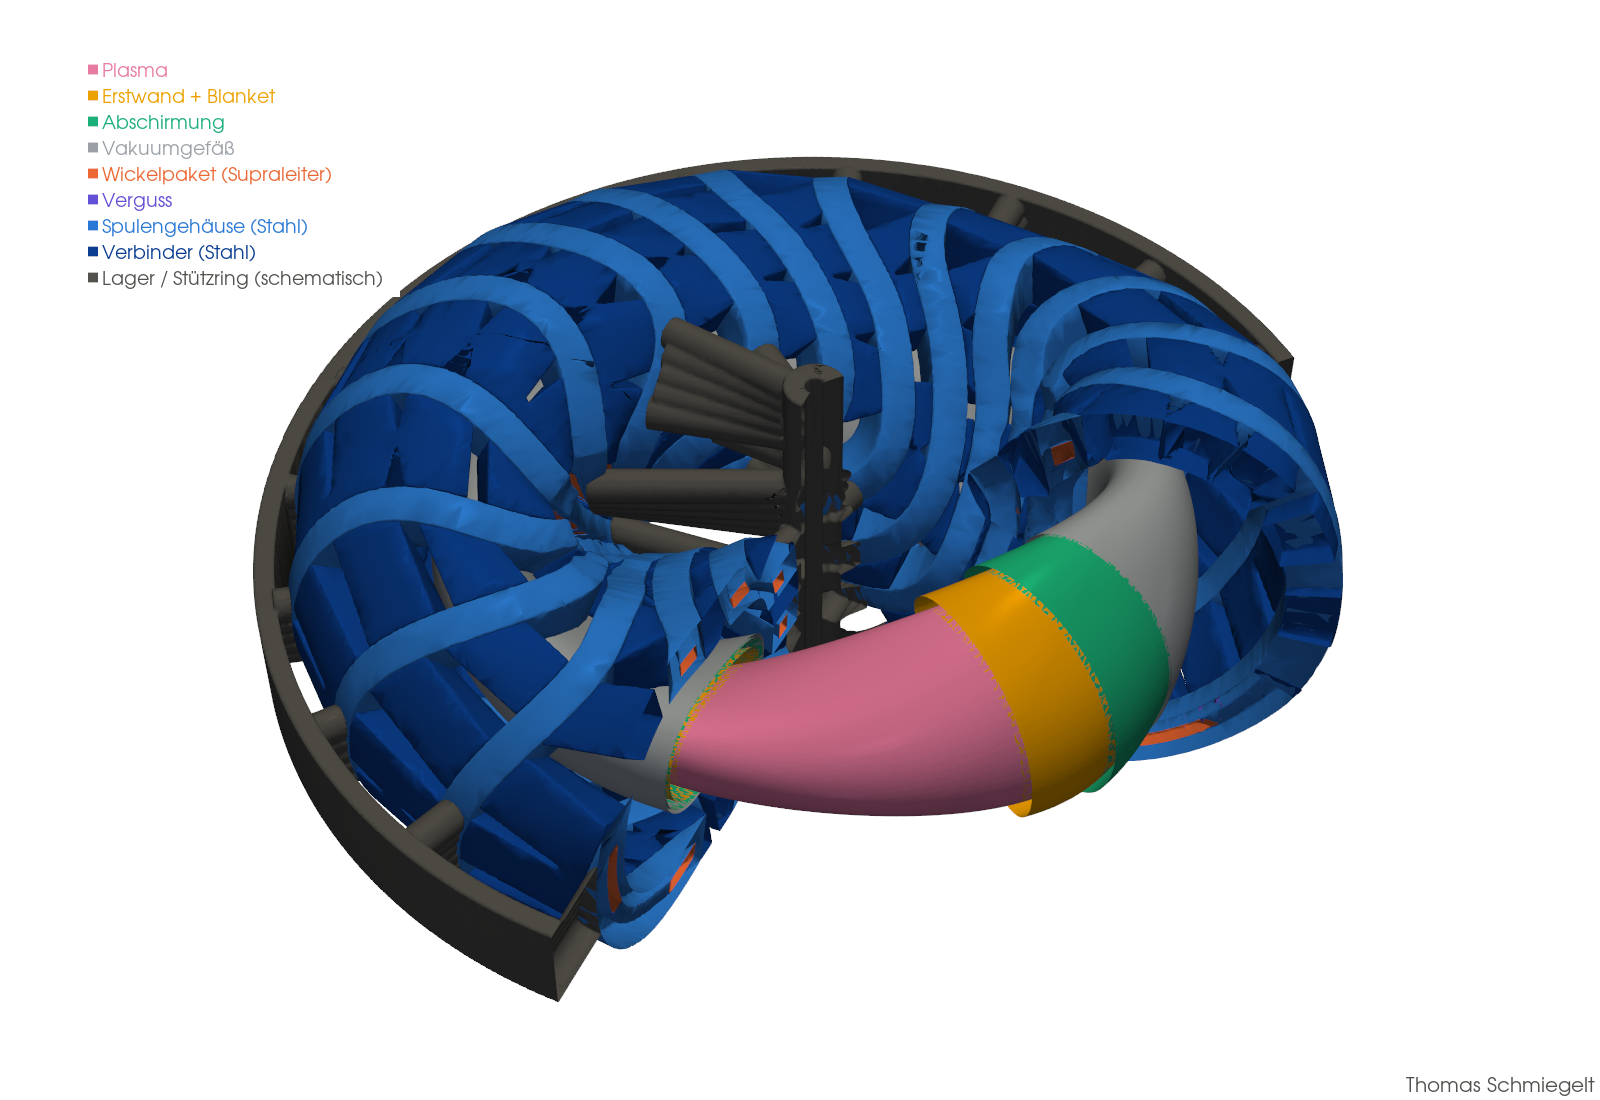
\includegraphics[width=\linewidth]{bilder/modell3d_0063_schnitt.png}\\\footnotesize PicoGK-Modell, Treppenschnitt\end{minipage}\hfill
\caption{Entwurf 0063}\end{figure}
\clearpage
\subsection{Entwurf 0136}\label{sb:0136}
\noindent\textbf{Urteil: }In doe1 zulässig, mit Standardnetz nicht mehr: Engpass Stahl σ99 (Reserve -15 \%).\par\smallskip
\begin{minipage}[t]{0.46\linewidth}\small\begin{tabular}[t]{@{}lr@{}}\toprule\multicolumn{2}{@{}l}{\textbf{Stellgrößen}}\\\midrule
Abstand Spule–Plasma & \num{0.232} \\
Spulen gesamt & 20 \\
Spulen je halbe Periode & \num{5} \\
Länge je Spule & \num{4.51} \\
Kraftziel & \num{0.012} \\
Wand innen & \num{0.16} \\
Seitenwand & \num{0.30} \\
Außenwand min. & \num{0.57} \\
Außenwand Zusatz & \num{0.22} \\
Verbindersteifigkeit & \num{21} \\
Verbinder je Paar & \num{13} \\
Lagerradius & \num{3.12} \\
\bottomrule\end{tabular}\end{minipage}\hfill
\begin{minipage}[t]{0.5\linewidth}\small\begin{tabular}[t]{@{}lr@{}}\toprule\multicolumn{2}{@{}l}{\textbf{Ergebnisse}}\\\midrule
$\sigma_{99}$ Stahl & \num{577} MPa \\
größtes Element & \num{2238} MPa \\
$P_m$ max. / 99 \% & \num{2201} / \num{690} MPa \\
$P_m+P_b$ max. & \num{2291} MPa \\
Verbinder σ99 & \num{141} MPa \\
Verformung max. & \num{54} mm \\
Dehnung Wickelpaket & \num{0.30} \% \\
Strom je Spule & \num{17.7} MA \\
Feld am Leiter & \num{16.9} T \\
Auslastung / Marge & \num{32} \% / \num{23} K \\
Feldfehler $B\cdot n$ & \num{1.62} ‰ \\
Freiraum Plasma–Gehäuse & \num{1.84} m \\
Kernheizung / Fluenz & \num{1} W/m³ / 9.6e15 \\
Stahl Gehäuse + Verbinder & \num{10.0} + \num{16.3} kt \\
Verbinder gebaut & 254 \\
\bottomrule\end{tabular}\end{minipage}\par\medskip
\noindent\textit{Netzstudie ($\sigma_{99}$/max. in MPa): }doe1: 479/995; Standard: 577/2238.\par\smallskip
\begin{figure}[H]\centering
\begin{minipage}[t]{0.49\linewidth}\centering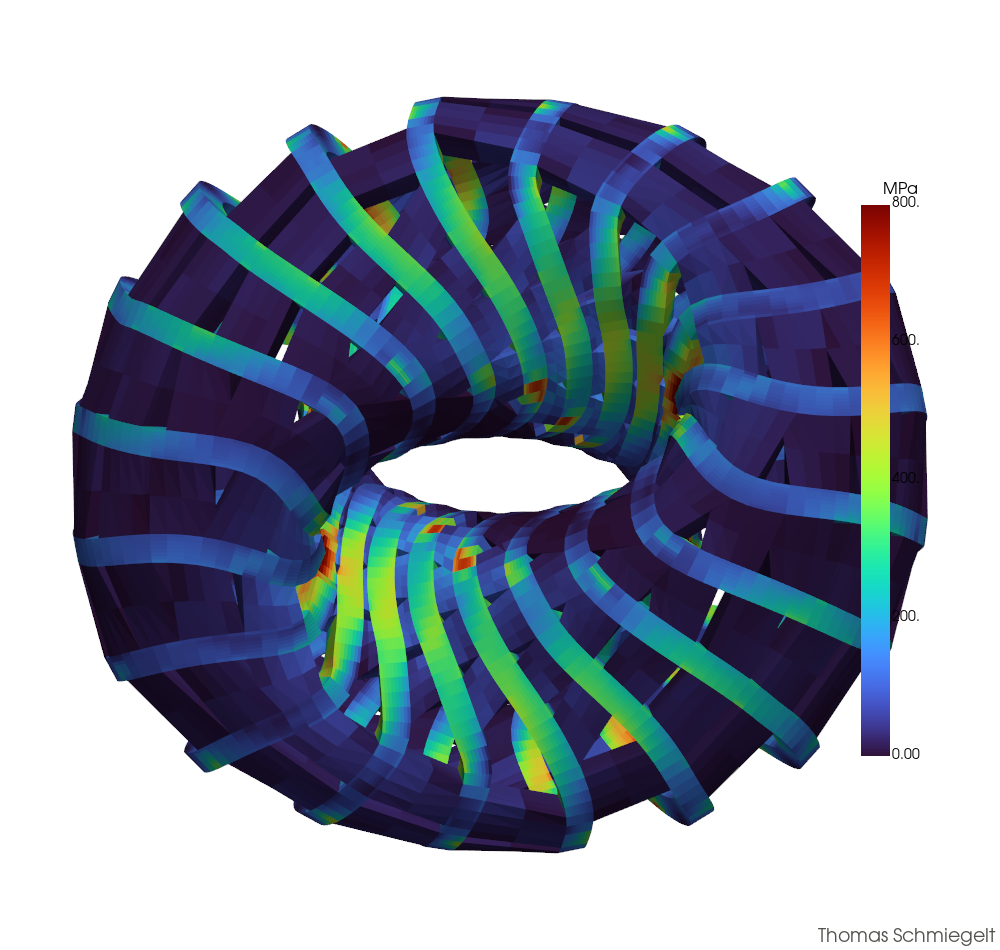
\includegraphics[width=\linewidth]{bilder/spannung_0136.png}\\\footnotesize Vergleichsspannung im Stahl (Draufsicht, 0–800 MPa)\end{minipage}\hfill
\begin{minipage}[t]{0.49\linewidth}\centering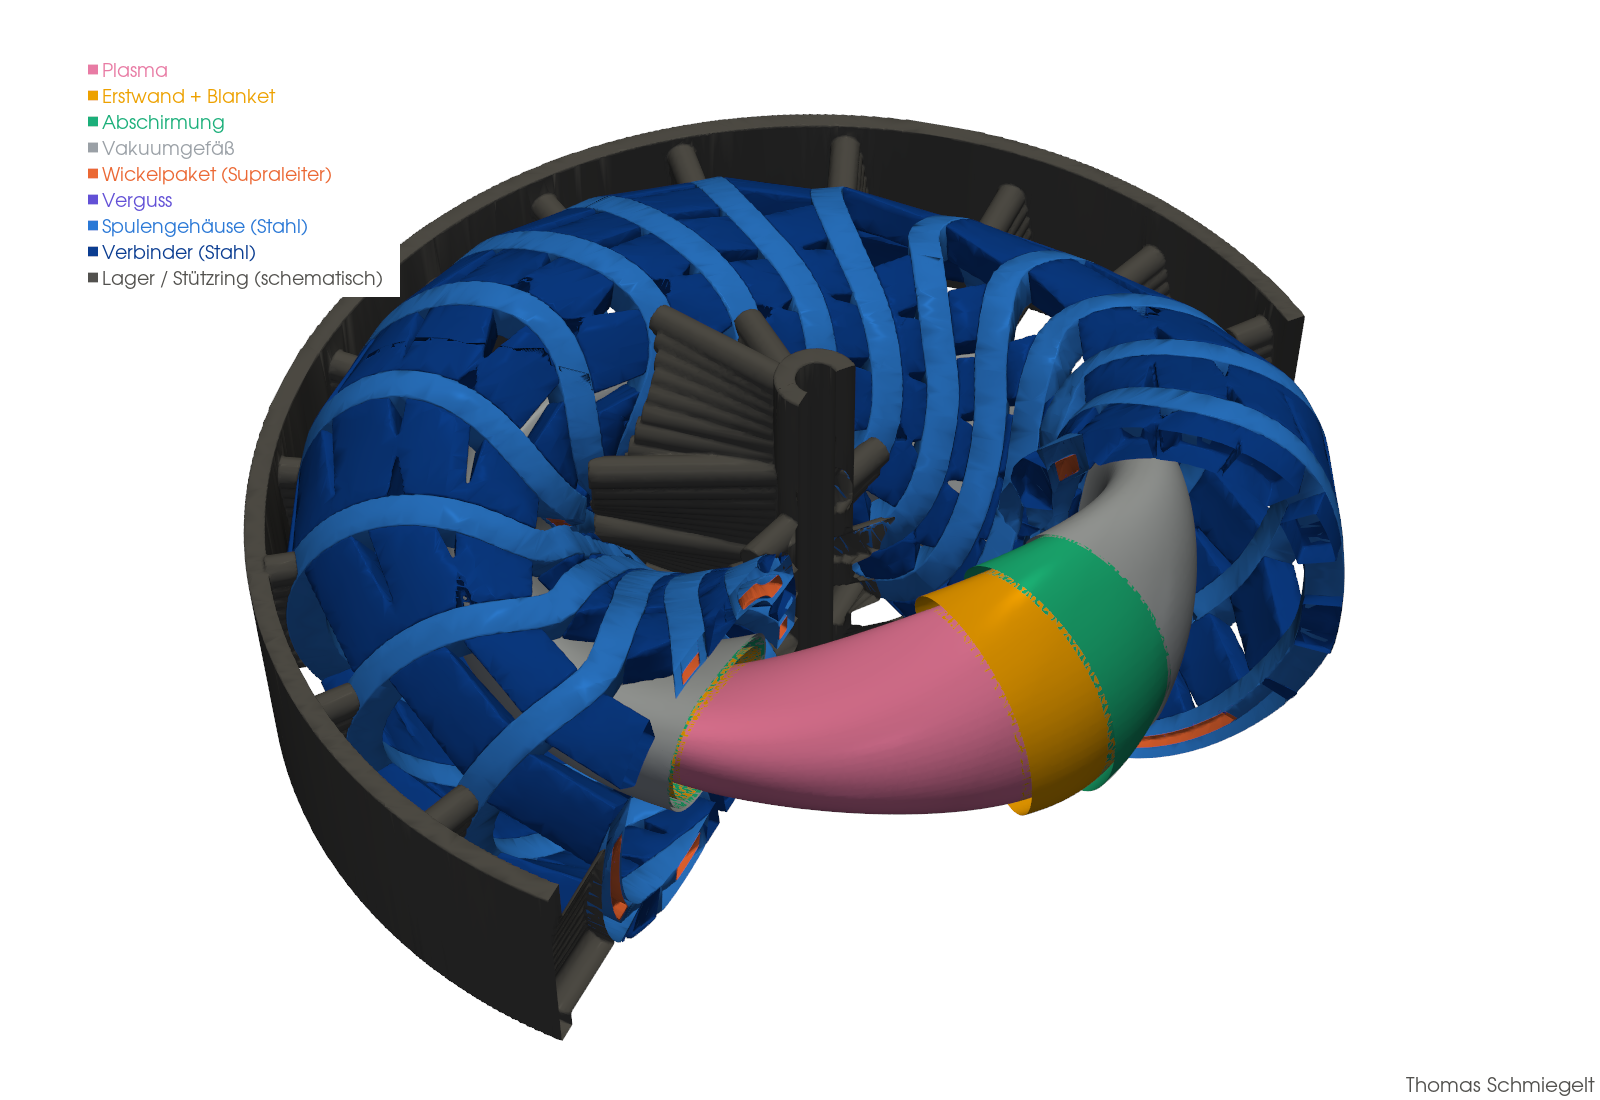
\includegraphics[width=\linewidth]{bilder/modell3d_0136_schnitt.png}\\\footnotesize PicoGK-Modell, Treppenschnitt\end{minipage}\hfill
\caption{Entwurf 0136}\end{figure}
\clearpage
\subsection{Vorschlag V3 des Ersatzmodells}\label{sb:V3}
\noindent\textbf{Urteil: }Vorschlag des Ersatzmodells (Abschnitt~\ref{sec:ersatz1}), zulässig; kleinste Reserve 35 \% (Feldfehler B·n).\par\smallskip
\begin{minipage}[t]{0.46\linewidth}\small\begin{tabular}[t]{@{}lr@{}}\toprule\multicolumn{2}{@{}l}{\textbf{Stellgrößen}}\\\midrule
Abstand Spule–Plasma & \num{0.205} \\
Spulen gesamt & 24 \\
Spulen je halbe Periode & \num{6} \\
Länge je Spule & \num{4.15} \\
Kraftziel & \num{0.022} \\
Wand innen & \num{0.20} \\
Seitenwand & \num{0.24} \\
Außenwand min. & \num{0.77} \\
Außenwand Zusatz & \num{0.48} \\
Verbindersteifigkeit & \num{176} \\
Verbinder je Paar & \num{11} \\
Lagerradius & \num{3.02} \\
\bottomrule\end{tabular}\end{minipage}\hfill
\begin{minipage}[t]{0.5\linewidth}\small\begin{tabular}[t]{@{}lr@{}}\toprule\multicolumn{2}{@{}l}{\textbf{Ergebnisse}}\\\midrule
$\sigma_{99}$ Stahl & \num{272} MPa \\
größtes Element & \num{656} MPa \\
$P_m$ max. / 99 \% & \num{621} / \num{302} MPa \\
$P_m+P_b$ max. & \num{724} MPa \\
Verbinder σ99 & \num{178} MPa \\
Verformung max. & \num{13} mm \\
Dehnung Wickelpaket & \num{0.13} \% \\
Strom je Spule & \num{14.7} MA \\
Feld am Leiter & \num{15.6} T \\
Auslastung / Marge & \num{30} \% / \num{24} K \\
Feldfehler $B\cdot n$ & \num{1.96} ‰ \\
Freiraum Plasma–Gehäuse & \num{1.54} m \\
Kernheizung / Fluenz & \num{22} W/m³ / 1.8e17 \\
Stahl Gehäuse + Verbinder & \num{12.3} + \num{16.8} kt \\
Verbinder gebaut & 256 \\
\bottomrule\end{tabular}\end{minipage}\par\medskip
\noindent\textit{Netzstudie ($\sigma_{99}$/max. in MPa): }Standard: 272/656; 1,5× Stationen: 394/1841.\par\smallskip
\begin{figure}[H]\centering
\begin{minipage}[t]{0.49\linewidth}\centering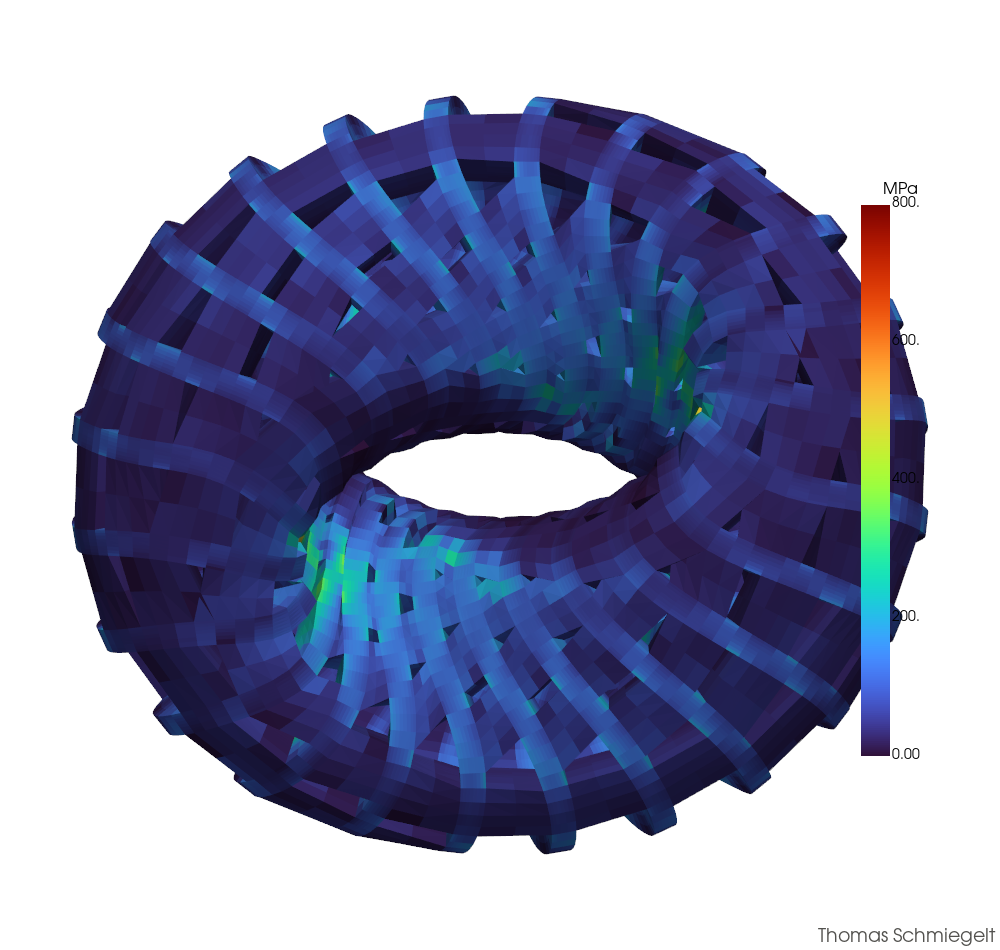
\includegraphics[width=\linewidth]{bilder/spannung_V3.png}\\\footnotesize Vergleichsspannung im Stahl (Draufsicht, 0–800 MPa)\end{minipage}\hfill
\begin{minipage}[t]{0.49\linewidth}\centering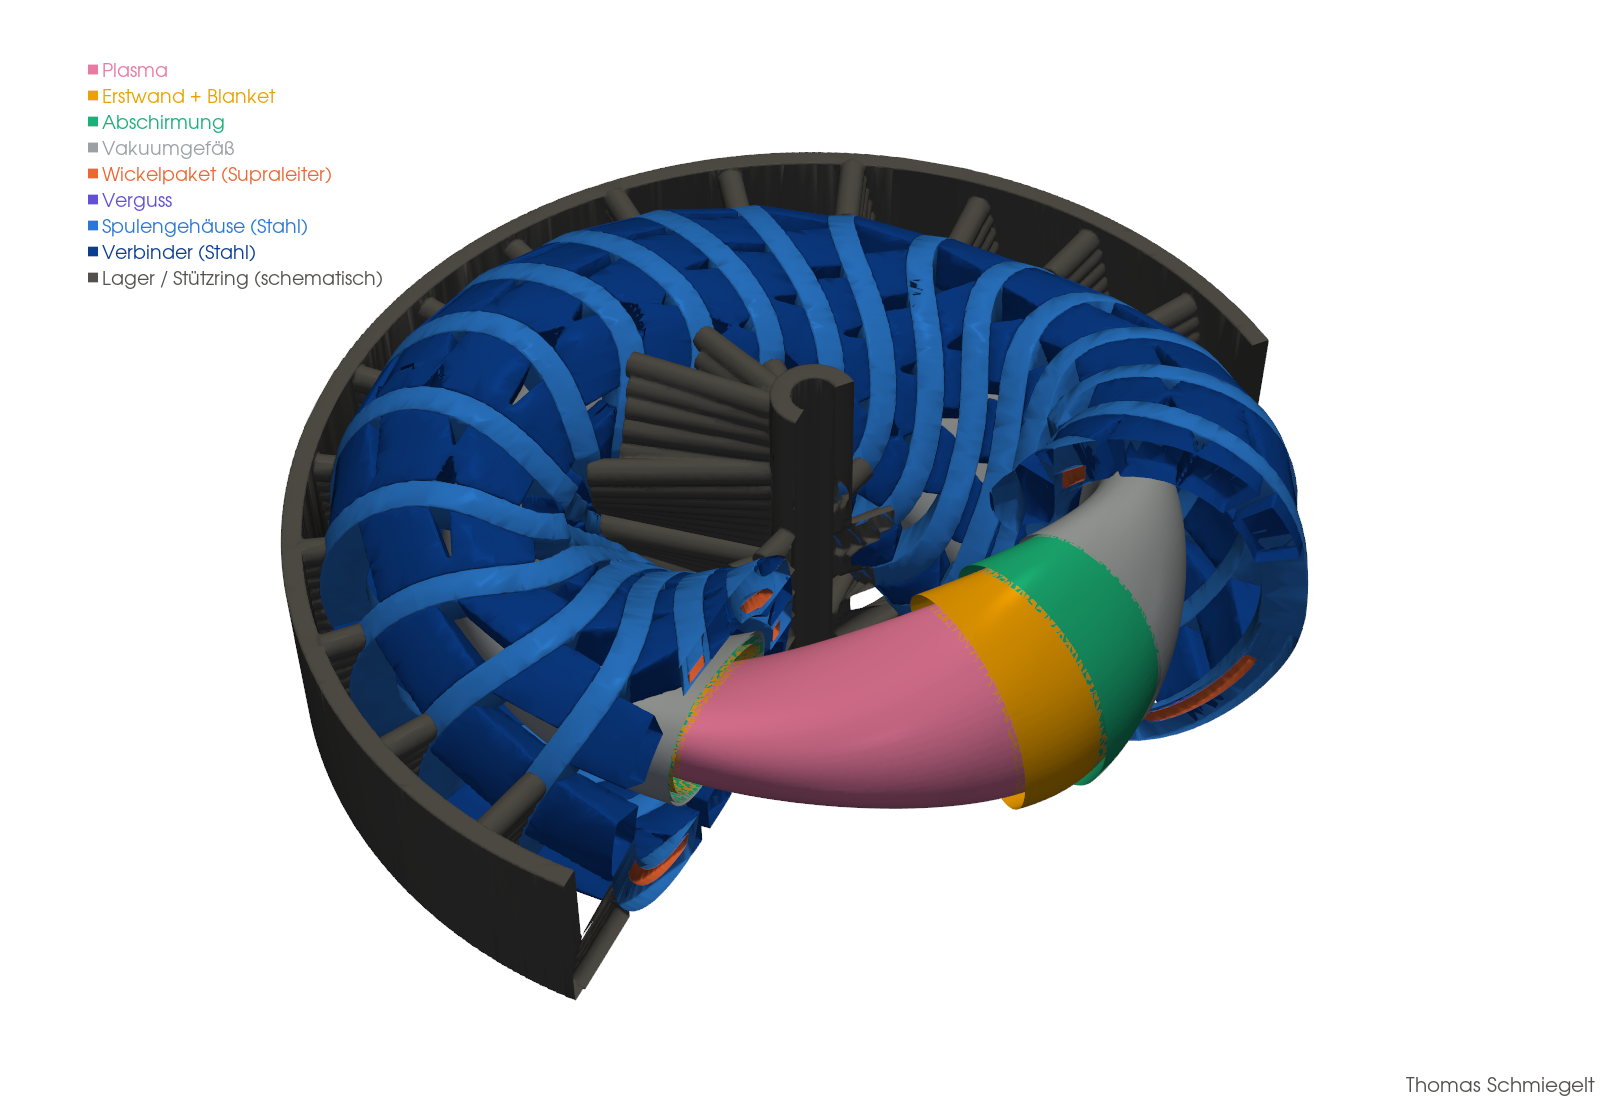
\includegraphics[width=\linewidth]{bilder/modell3d_V3_schnitt.png}\\\footnotesize PicoGK-Modell, Treppenschnitt\end{minipage}\hfill
\caption{Vorschlag V3 des Ersatzmodells}\end{figure}
\clearpage
\subsection{Vorschlag V1 des Ersatzmodells}\label{sb:V1}
\noindent\textbf{Urteil: }Vorschlag des Ersatzmodells (Abschnitt~\ref{sec:ersatz1}), zulässig; kleinste Reserve 31 \% (Platz Package).\par\smallskip
\begin{minipage}[t]{0.46\linewidth}\small\begin{tabular}[t]{@{}lr@{}}\toprule\multicolumn{2}{@{}l}{\textbf{Stellgrößen}}\\\midrule
Abstand Spule–Plasma & \num{0.208} \\
Spulen gesamt & 24 \\
Spulen je halbe Periode & \num{6} \\
Länge je Spule & \num{3.98} \\
Kraftziel & \num{0.023} \\
Wand innen & \num{0.36} \\
Seitenwand & \num{0.32} \\
Außenwand min. & \num{0.77} \\
Außenwand Zusatz & \num{0.33} \\
Verbindersteifigkeit & \num{77} \\
Verbinder je Paar & \num{13} \\
Lagerradius & \num{3.41} \\
\bottomrule\end{tabular}\end{minipage}\hfill
\begin{minipage}[t]{0.5\linewidth}\small\begin{tabular}[t]{@{}lr@{}}\toprule\multicolumn{2}{@{}l}{\textbf{Ergebnisse}}\\\midrule
$\sigma_{99}$ Stahl & \num{220} MPa \\
größtes Element & \num{637} MPa \\
$P_m$ max. / 99 \% & \num{532} / \num{248} MPa \\
$P_m+P_b$ max. & \num{746} MPa \\
Verbinder σ99 & \num{111} MPa \\
Verformung max. & \num{11} mm \\
Dehnung Wickelpaket & \num{0.12} \% \\
Strom je Spule & \num{14.7} MA \\
Feld am Leiter & \num{15.6} T \\
Auslastung / Marge & \num{30} \% / \num{24} K \\
Feldfehler $B\cdot n$ & \num{1.87} ‰ \\
Freiraum Plasma–Gehäuse & \num{1.41} m \\
Kernheizung / Fluenz & \num{85} W/m³ / 7.1e17 \\
Stahl Gehäuse + Verbinder & \num{14.6} + \num{18.5} kt \\
Verbinder gebaut & 308 \\
\bottomrule\end{tabular}\end{minipage}\par\medskip
\noindent\textit{Netzstudie ($\sigma_{99}$/max. in MPa): }Standard: 220/637; 1,5× Stationen: 366/2185.\par\smallskip
\begin{figure}[H]\centering
\begin{minipage}[t]{0.49\linewidth}\centering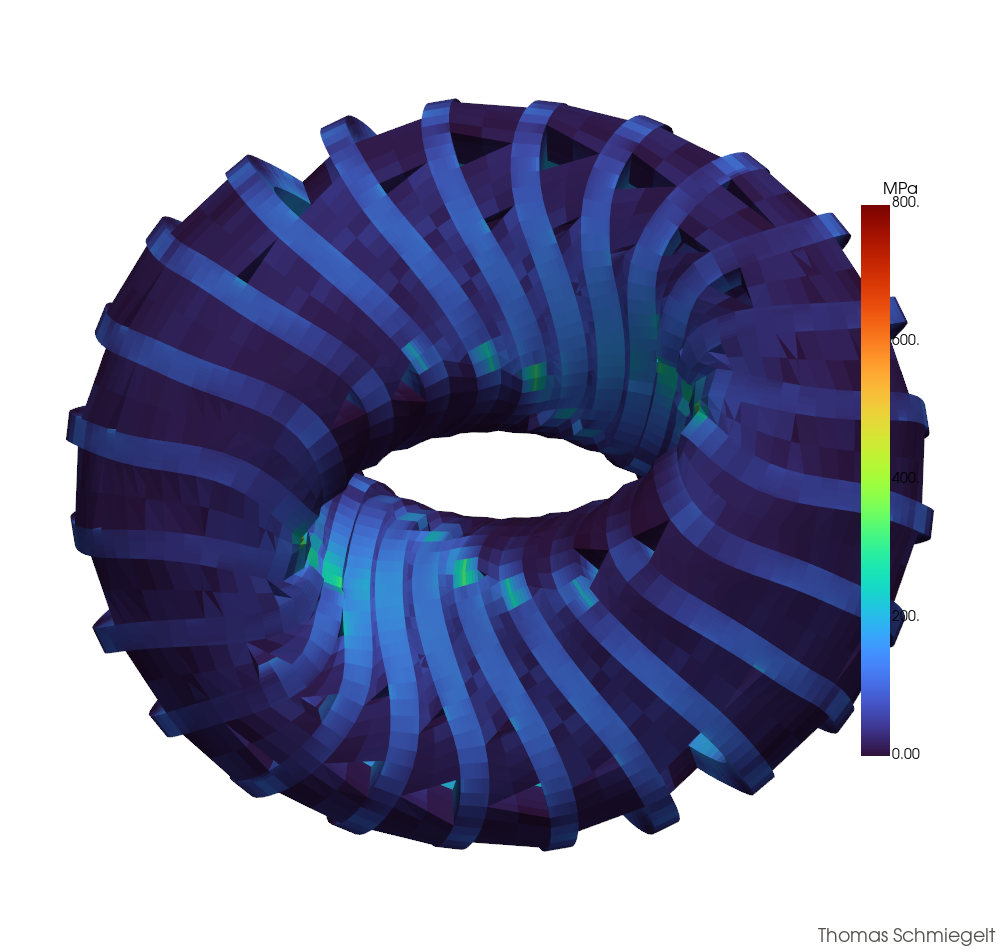
\includegraphics[width=\linewidth]{bilder/spannung_V1.png}\\\footnotesize Vergleichsspannung im Stahl (Draufsicht, 0–800 MPa)\end{minipage}\hfill
\begin{minipage}[t]{0.49\linewidth}\centering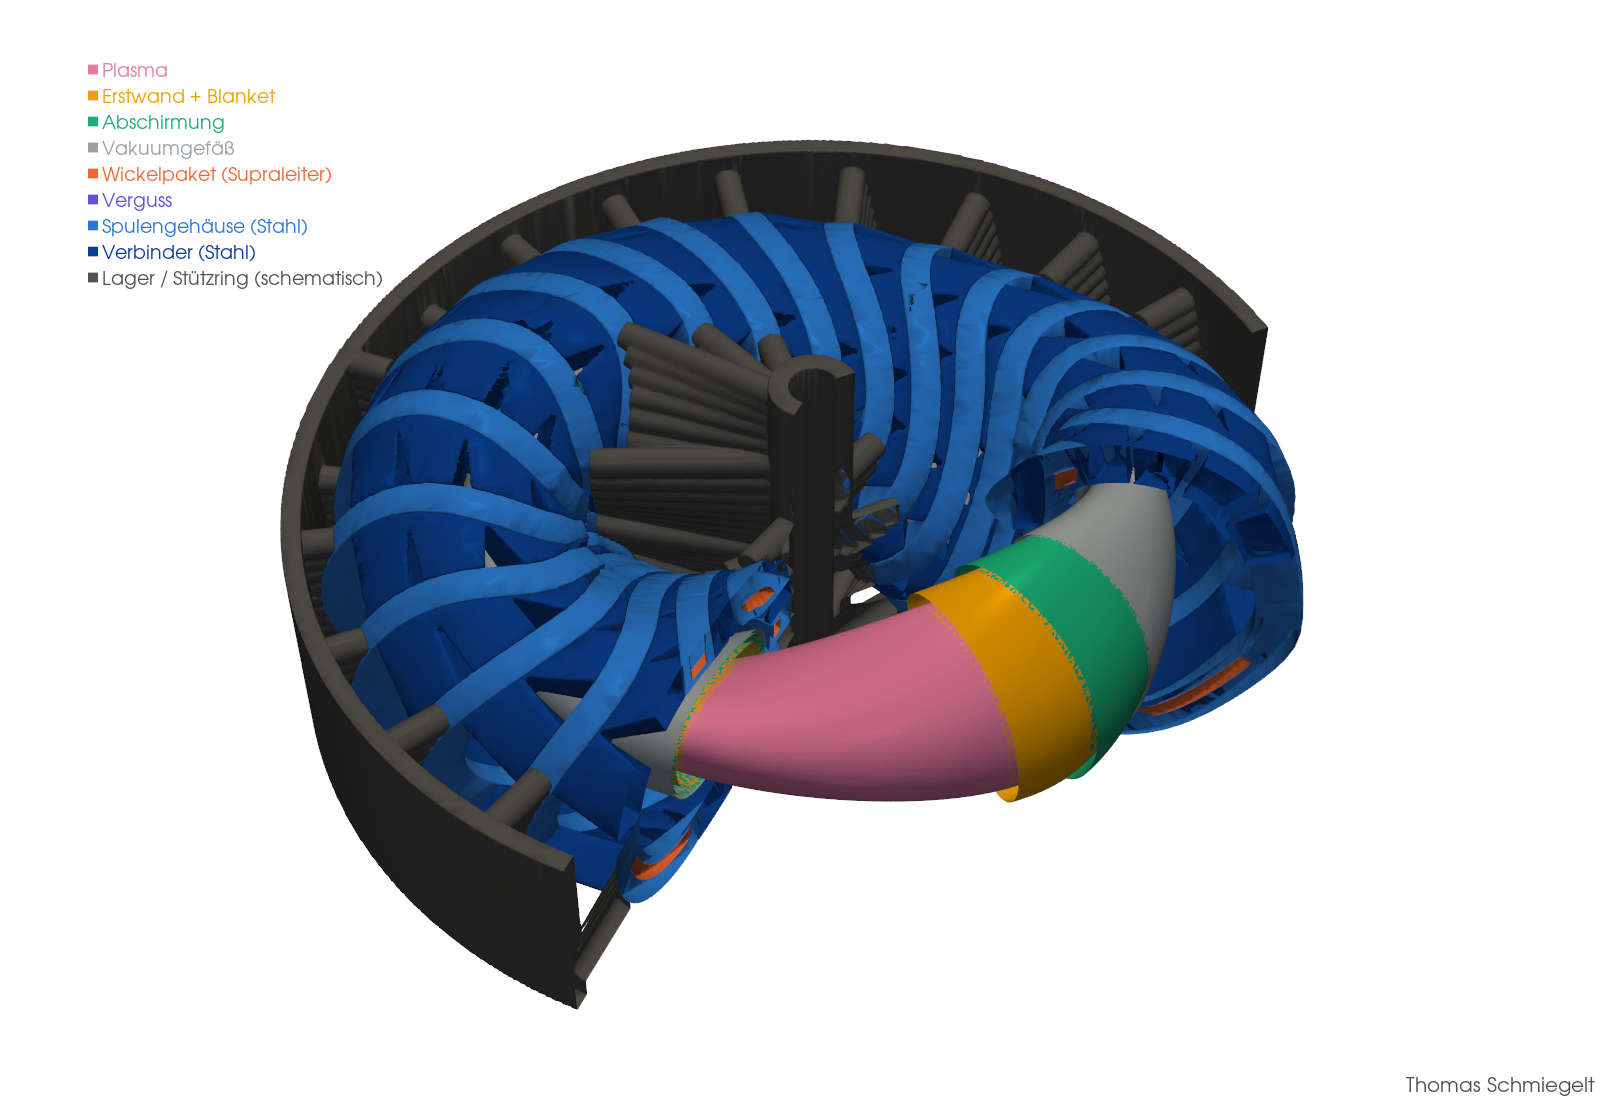
\includegraphics[width=\linewidth]{bilder/modell3d_V1_schnitt.png}\\\footnotesize PicoGK-Modell, Treppenschnitt\end{minipage}\hfill
\caption{Vorschlag V1 des Ersatzmodells}\end{figure}
\clearpage
\subsection{Tragwerksversuch E (dickste Wände)}\label{sb:E_test}
\noindent\textbf{Urteil: }Gleiche 16 Spulen wie der Ausgangsentwurf; nur das Tragwerk ist verändert.\par\smallskip
\begin{minipage}[t]{0.46\linewidth}\small\begin{tabular}[t]{@{}lr@{}}\toprule\multicolumn{2}{@{}l}{\textbf{Stellgrößen}}\\\midrule
Abstand Spule–Plasma & \num{0.180} \\
Spulen gesamt & 16 \\
Spulen je halbe Periode & \num{4} \\
Länge je Spule & \num{4.50} \\
Kraftziel & \num{0.000} \\
Wand innen & \num{0.60} \\
Seitenwand & \num{0.40} \\
Außenwand min. & \num{0.80} \\
Außenwand Zusatz & \num{0.60} \\
Verbindersteifigkeit & \num{200} \\
Verbinder je Paar & \num{12} \\
Lagerradius & \num{2.50} \\
\bottomrule\end{tabular}\end{minipage}\hfill
\begin{minipage}[t]{0.5\linewidth}\small\begin{tabular}[t]{@{}lr@{}}\toprule\multicolumn{2}{@{}l}{\textbf{Ergebnisse}}\\\midrule
$\sigma_{99}$ Stahl & \num{481} MPa \\
größtes Element & \num{2455} MPa \\
$P_m$ max. / 99 \% & \num{2396} / \num{736} MPa \\
$P_m+P_b$ max. & \num{2515} MPa \\
Verbinder σ99 & \num{276} MPa \\
Verformung max. & \num{41} mm \\
Dehnung Wickelpaket & \num{0.31} \% \\
Strom je Spule & \num{22.1} MA \\
Feld am Leiter & \num{18.7} T \\
Auslastung / Marge & \num{34} \% / \num{22} K \\
Feldfehler $B\cdot n$ & \num{2.71} ‰ \\
Freiraum Plasma–Gehäuse & \num{1.53} m \\
Kernheizung / Fluenz & \num{25} W/m³ / 2.1e17 \\
Stahl Gehäuse + Verbinder & \num{17.6} + \num{19.4} kt \\
Verbinder gebaut & 168 \\
\bottomrule\end{tabular}\end{minipage}\par\medskip
\begin{figure}[H]\centering
\begin{minipage}[t]{0.49\linewidth}\centering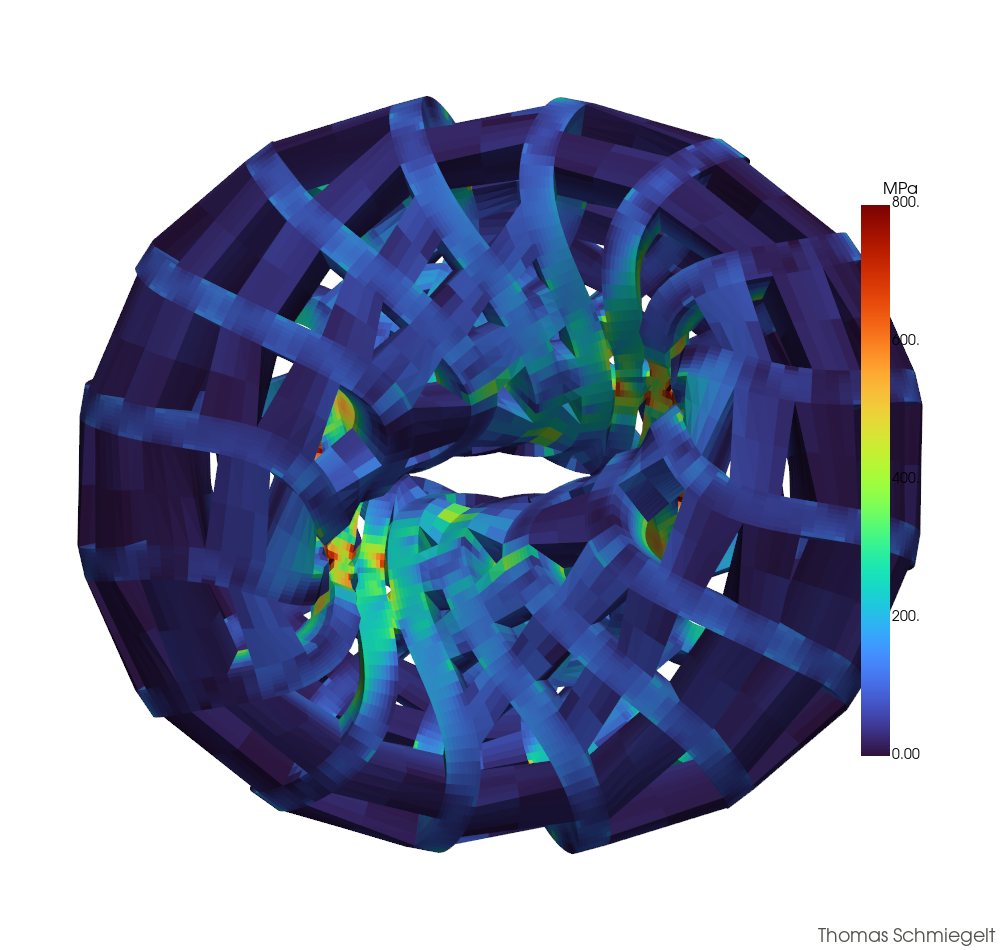
\includegraphics[width=\linewidth]{bilder/spannung_E_test.png}\\\footnotesize Vergleichsspannung im Stahl (Draufsicht, 0–800 MPa)\end{minipage}\hfill
\begin{minipage}[t]{0.49\linewidth}\centering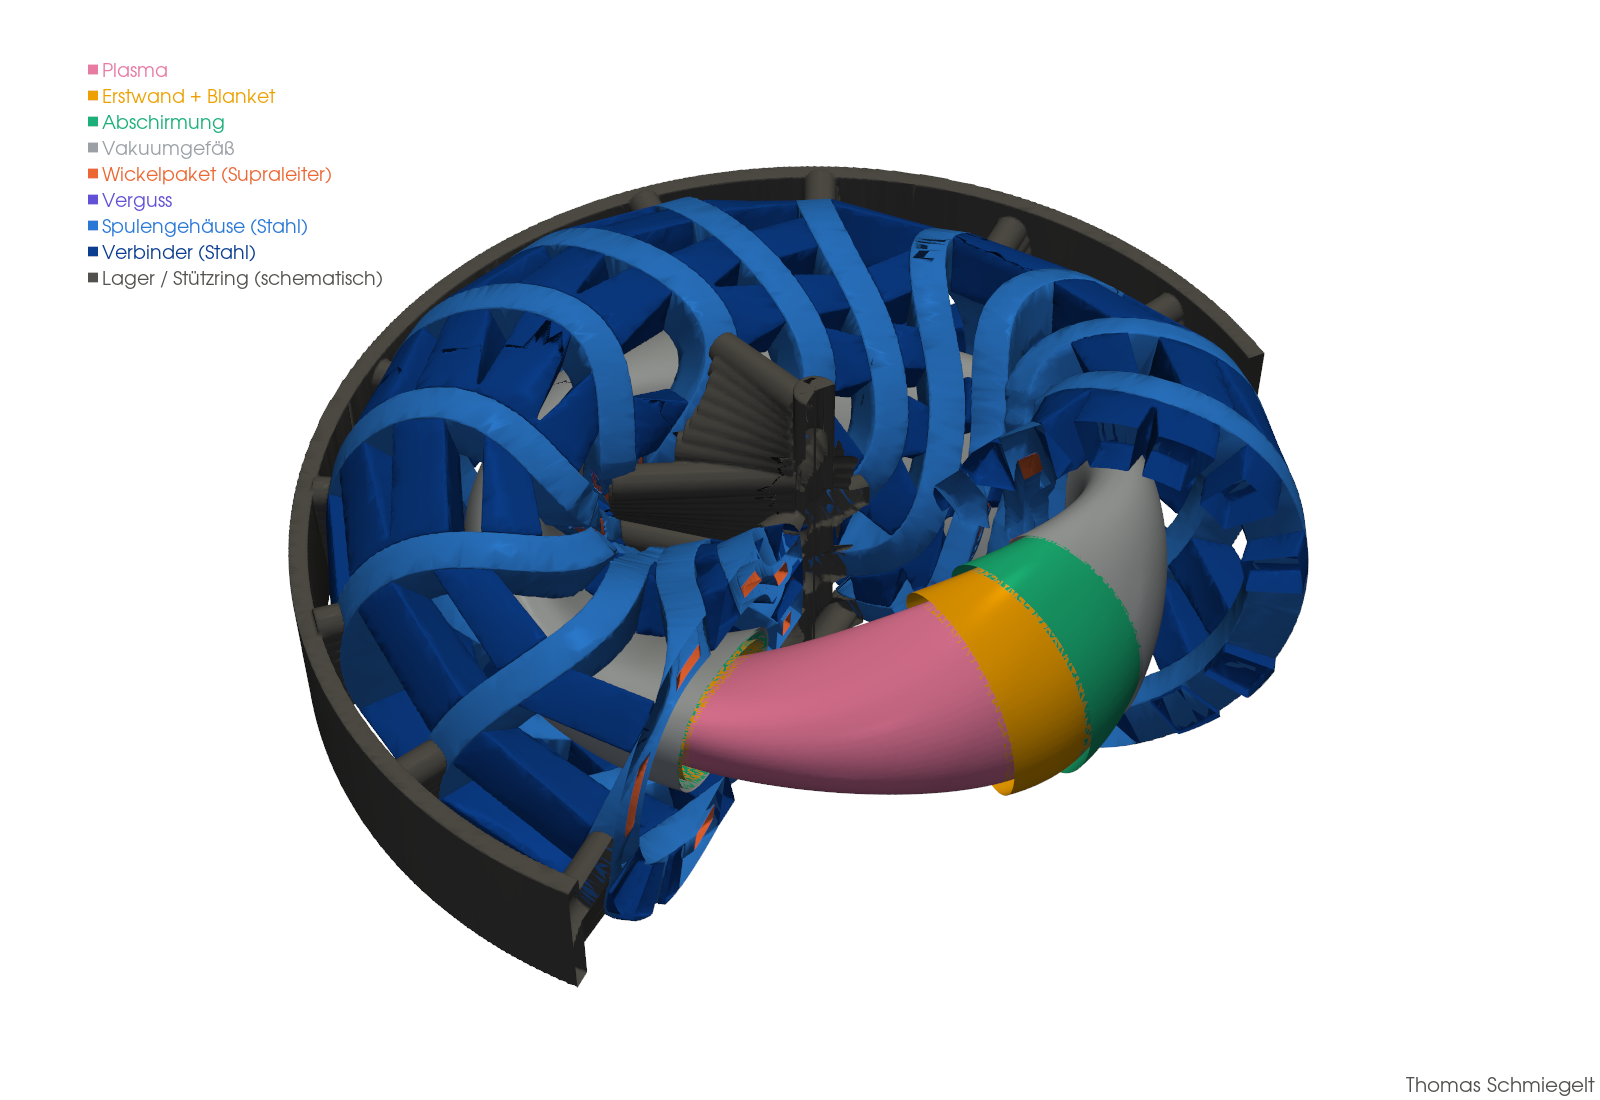
\includegraphics[width=\linewidth]{bilder/modell3d_E_test_schnitt.png}\\\footnotesize PicoGK-Modell, Treppenschnitt\end{minipage}\hfill
\caption{Tragwerksversuch E (dickste Wände)}\end{figure}
\clearpage
\subsection{Tragwerksversuch A (Ausgangsentwurf)}\label{sb:A_test}
\noindent\textbf{Urteil: }Gleiche 16 Spulen wie der Ausgangsentwurf; nur das Tragwerk ist verändert.\par\smallskip
\begin{minipage}[t]{0.46\linewidth}\small\begin{tabular}[t]{@{}lr@{}}\toprule\multicolumn{2}{@{}l}{\textbf{Stellgrößen}}\\\midrule
Abstand Spule–Plasma & \num{0.180} \\
Spulen gesamt & 16 \\
Spulen je halbe Periode & \num{4} \\
Länge je Spule & \num{4.50} \\
Kraftziel & \num{0.000} \\
Wand innen & \num{0.35} \\
Seitenwand & \num{0.24} \\
Außenwand min. & \num{0.45} \\
Außenwand Zusatz & \num{0.30} \\
Verbindersteifigkeit & \num{50} \\
Verbinder je Paar & \num{6} \\
Lagerradius & \num{2.50} \\
\bottomrule\end{tabular}\end{minipage}\hfill
\begin{minipage}[t]{0.5\linewidth}\small\begin{tabular}[t]{@{}lr@{}}\toprule\multicolumn{2}{@{}l}{\textbf{Ergebnisse}}\\\midrule
$\sigma_{99}$ Stahl & \num{2129} MPa \\
größtes Element & \num{8454} MPa \\
Verbinder σ99 & \num{675} MPa \\
Verformung max. & \num{399} mm \\
Dehnung Wickelpaket & \num{0.76} \% \\
Strom je Spule & \num{22.1} MA \\
Feld am Leiter & \num{18.7} T \\
Auslastung / Marge & \num{34} \% / \num{22} K \\
Feldfehler $B\cdot n$ & \num{2.71} ‰ \\
Freiraum Plasma–Gehäuse & \num{1.77} m \\
Kernheizung / Fluenz & \num{2} W/m³ / 1.8e16 \\
Stahl Gehäuse + Verbinder & \num{8.5} + \num{7.0} kt \\
Verbinder gebaut & 90 \\
\bottomrule\end{tabular}\end{minipage}\par\medskip
\begin{figure}[H]\centering
\begin{minipage}[t]{0.49\linewidth}\centering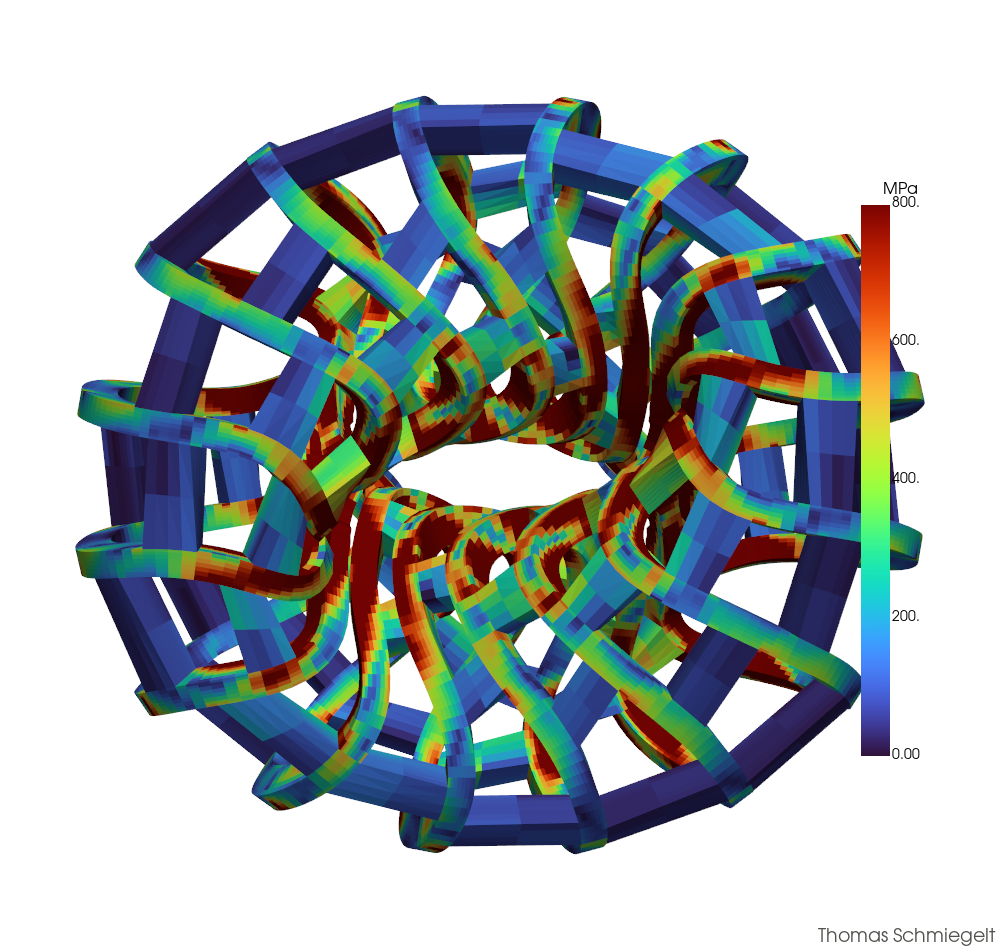
\includegraphics[width=\linewidth]{bilder/spannung_A_test.png}\\\footnotesize Vergleichsspannung im Stahl (Draufsicht, 0–800 MPa)\end{minipage}\hfill
\begin{minipage}[t]{0.49\linewidth}\centering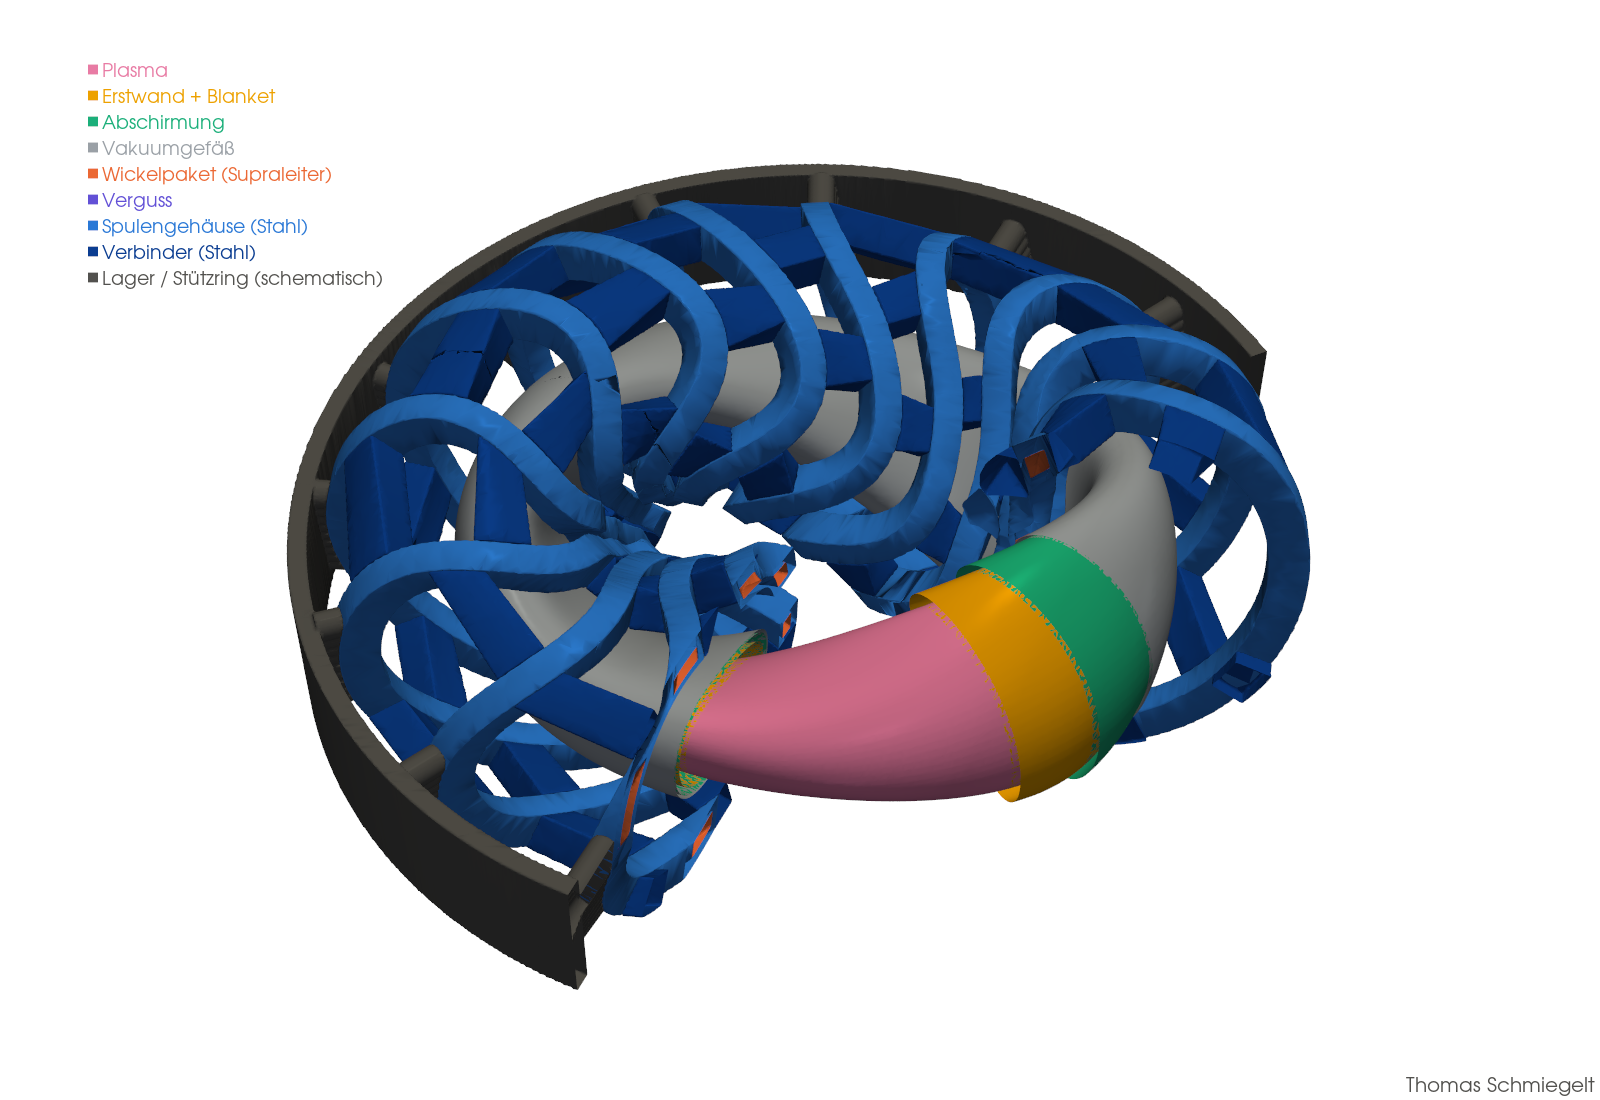
\includegraphics[width=\linewidth]{bilder/modell3d_A_test_schnitt.png}\\\footnotesize PicoGK-Modell, Treppenschnitt\end{minipage}\hfill
\caption{Tragwerksversuch A (Ausgangsentwurf)}\end{figure}


%======================================================================
\section{Vergleich und Folgerungen}\label{sec:vergleich}
\paragraph{Welcher Entwurf ist der robusteste?} Gesucht war auf Wunsch des Nutzers nicht der leichteste, sondern der
Entwurf mit der größten Reserve gegen alle acht Grenzen („das Gewicht ist nicht so wichtig, es ist ja ein
Gebäude“). Nach der Bereinigung erfüllen sieben Entwürfe alle Grenzen. Ihre kleinste Reserve (Robustheit) liegt
zwischen 0,30 (0061) und 0,02 (0157). Zwei Entwürfe liegen fast gleichauf: 0061 (Engpass Stahl) und 0169 (Engpass
Package-Dicke). Entscheidend ist die Netzstudie (Abschnitt~\ref{sec:netz}):

\begin{itemize}
\item \textbf{0169} bleibt bei feinerem Netz praktisch gleich (\SI{308}{} $\to$ \SI{319}{MPa}, $+4$~\%). Seine
  Reserve hängt nicht an der Rechengenauigkeit. Engpass ist die Package-Dicke, die von der Geometrie, nicht vom
  Netz abhängt. Er ist deshalb der \textbf{empfohlene Entwurf}: 24 Spulen, 13 steife Verbinder je Spulenpaar,
  rund \SI{28}{kt} Stahl.
\item \textbf{0061} hat zwar die größte Reserve im Standardnetz, seine Spannung steigt aber im feinen Netz um 58~\%
  (\SI{351}{} $\to$ \SI{556}{MPa}) und überschreitet dann die Grenze. Sein Engpass ist gerade die netzabhängige
  Größe.
\item \textbf{0093, 0008, 0014} steigen im feinen Netz um 34--46~\% und bleiben teils knapp darunter, teils
  darüber. Sie sind Kandidaten, aber erst nach einer genaueren Rechnung der Verbinderanschlüsse.
\item \textbf{0017, 0157} haben wenig Reserve und wurden nicht weiter verfeinert.
\item \textbf{V3, V1} (Vorschläge des Ersatzmodells) sind im Standardnetz robuster als 0169 (0,35 und 0,31), im
  feinen Netz steigt ihre Spannung aber um 45 bzw.\ 66~\% (Abschnitt~\ref{sec:ersatz1}). V3 fällt damit auf 0,21.
\end{itemize}

\paragraph{Knapp verfehlt.} Die fünf Entwürfe mit der höchsten Robustheit unter den unzulässigen (0173, 0103, 0044,
0004, 0136) scheitern fast alle an der Stahlspannung oder am Feldfehler $B_n$. 0063 und 0136 waren mit dem groben
Netz zulässig und fielen nach der Nachrechnung heraus -- ein Beispiel dafür, wie leicht ein unbemerkt anderes Netz
das Ergebnis schönt.

\paragraph{Was die Varianten unterscheidet.} Über alle 198 Entwürfe hinweg gilt:
\begin{enumerate}
\item \textbf{Spulenzahl:} Mit 16 Spulen war kein Entwurf zulässig. Die Spulen werden dann so lang und so stark
  gekrümmt, dass die Gehäuse sich zu sehr biegen; zugleich ist der Feldfehler größer. 20 und 24 Spulen teilen die
  Kraft auf mehr und kürzere Bauteile.
\item \textbf{Spulenform vor Tragwerk:} Abstand Spule--Plasma und Spulenlänge bestimmen die Spannung stärker als
  Zahl oder Steifigkeit der Verbinder. Das Tragwerk kann eine ungünstige Spulenform nur begrenzt ausgleichen.
\item \textbf{Package und Kernheizung} sind fast reine Geometriefragen und werden vom Ersatzmodell sehr gut
  vorhergesagt ($R^2 \approx 0{,}98$). Sie lassen sich schon vor einer Festigkeitsrechnung sicher aussortieren.
\item \textbf{Die Spannung} wird vom Ersatzmodell nur grob getroffen ($R^2 \approx 0{,}46$), weil sie an örtlichen
  Spitzen am Verbinderanschluss hängt. Hier bleibt die FE-Rechnung unverzichtbar.
\item \textbf{Weichere Verbinder} (Nutzer-Idee „gezielt schwächen“, erste Form) erhöhen die Spannung. Die Idee muss
  örtlich umgesetzt werden: weiche Anschlüsse, steifer Kern.
\end{enumerate}

\paragraph{Wie belastbar ist das?} Die Zahlen stammen aus einem vereinfachten Modell: Gehäuse als
Rechteckquerschnitt, Verbinder als Balkenpakete, Lager als feste Punkte, nur die Magnetkraft im kalten Betrieb
(keine Abkühlspannung, kein Gewicht, keine Ermüdung). Das feinere Netz zeigt, dass die Spitzen noch nicht
konvergiert sind. Die Aussage „0169 ist robust, 16 Spulen gehen nicht“ ist belastbar, weil sie in allen Netzen
gilt; die genauen Megapascal sind es noch nicht.

\paragraph{Nächste Schritte.}
\begin{enumerate}
\item 0169 mit örtlich gestuften Verbindern (weiche Enden) und gerundeten Anschlüssen rechnen; Steifigkeiten
  iterativ nach dem Spannungsverhältnis anpassen.
\item Die Vermutung prüfen, dass 0169 netzstabil ist, weil seine Verbinder zu fast durchgehenden Platten
  verschmelzen: 0169 einmal mit überschneidungsfreien Verbindern, einmal mit bewusst durchgehender Platte rechnen.
\item Netzkonvergenz am Verbinderanschluss für 0169 und 0093 mit gezielter örtlicher Verfeinerung prüfen.
\item Abkühlspannung (\SI{293}{K} $\to$ \SI{4}{K}) und Eigengewicht ergänzen.
\item Das PicoGK-Modell von 0169 als Ausgangsform für Lager, Kühlkanäle und Verguss weiterverwenden.
\end{enumerate}


%======================================================================
\appendix
\section{Alle Entwürfe der Studie doe1}\label{anh:alle}
Abkürzungen: Sp.\ Spulen, Abst.\ Mindestabstand Spule--Plasma (Einheitsgeometrie), Länge je Spule
(Einheitsgeometrie), Kraft = Kraftgewicht, W.i./W.s.\ Wand innen/seitlich, t Außenwand min., n\textsubscript{V}
Verbinder je Paar, E\textsubscript{V} Verbindersteifigkeit, R\textsubscript{L} Lagerradius, frei = Freiraum
Plasma--Gehäuse, Kern = Kernheizung Wickelpaket. Letzte Spalte: \checkmark\ zulässig, sonst Engpass. $^\ast$ = mit
Standardnetz nachgerechnet.
{\scriptsize\setlength{\tabcolsep}{2.2pt}\begin{longtable}{@{}lrrrrrrrrrrrrrrrrrl@{}}\toprule
Nr. & Sp. & Abst. & Länge & Kraft & W.i. & W.s. & t & n\textsubscript{V} & E\textsubscript{V} & R\textsubscript{L} & $\sigma_{99}$ & max. & Dehn. & $B\cdot n$ & frei & Kern & Stahl & ok \\
 & & – & – & – & m & m & m & & GPa & m & MPa & MPa & \% & ‰ & m & W/m³ & kt & \\\midrule\endhead
0000 & 24 & \num{0.18} & \num{4.4} & \num{0.024} & \num{0.10} & \num{0.35} & \num{0.58} & 10 & \num{70} & \num{2.5} & \num{840} & \num{3425} & \num{0.42} & \num{1.98} & \num{1.44} & \num{60} & \num{23} & stahl \\
0001 & 20 & \num{0.24} & \num{4.4} & \num{0.012} & \num{0.13} & \num{0.15} & \num{0.35} & 7 & \num{135} & \num{2.9} & \num{1456} & \num{3851} & \num{0.60} & \num{1.53} & \num{2.00} & \num{0} & \num{12} & stahl \\
0002 & 24 & \num{0.30} & \num{4.5} & \num{0.028} & \num{0.26} & \num{0.10} & \num{0.20} & 8 & \num{25} & \num{2.7} & \num{4721} & \num{13357} & \num{2.01} & \num{3.67} & \num{2.39} & \num{0} & \num{13} & stahl \\
0003 & 16 & \num{0.20} & \num{3.7} & \num{0.025} & \num{0.34} & \num{0.10} & \num{0.49} & 12 & \num{142} & \num{1.9} & \num{617} & \num{1361} & \num{0.26} & \num{9.48} & \num{1.40} & \num{90} & \num{20} & Bn \\
0004 & 20 & \num{0.19} & \num{4.6} & \num{0.012} & \num{0.12} & \num{0.08} & \num{0.50} & 10 & \num{148} & \num{3.2} & \num{558} & \num{1085} & \num{0.26} & \num{1.81} & \num{1.54} & \num{22} & \num{19} & stahl \\
0005 & 16 & \num{0.15} & \num{4.9} & \num{0.020} & \num{0.59} & \num{0.08} & \num{0.15} & 13 & \num{114} & \num{2.9} & \num{844} & \num{1847} & \num{0.35} & \num{2.40} & \num{1.26} & \num{372} & \num{23} & stahl \\
0006 & 24 & \num{0.12} & \num{4.4} & \num{0.012} & \num{0.50} & \num{0.14} & \num{0.18} & 6 & \num{78} & \num{2.9} & \num{536} & \num{1222} & \num{0.22} & \num{1.77} & \num{0.99} & \num{5689} & \num{14} & fluenz \\
0007 & 16 & \num{0.16} & \num{3.7} & \num{0.019} & \num{0.14} & \num{0.38} & \num{0.36} & 8 & \num{88} & \num{2.6} & \num{870} & \num{3574} & \num{0.42} & \num{9.92} & \num{1.60} & \num{12} & \num{17} & Bn \\
0008 & 24 & \num{0.21} & \num{3.7} & \num{0.030} & \num{0.32} & \num{0.31} & \num{0.72} & 11 & \num{142} & \num{2.8} & \num{305} & \num{1695} & \num{0.17} & \num{2.20} & \num{1.48} & \num{40} & \num{26} & \checkmark \\
0009 & 24 & \num{0.23} & \num{4.1} & \num{0.008} & \num{0.49} & \num{0.25} & \num{0.28} & 13 & \num{145} & \num{3.0} & \num{1159} & \num{9216} & \num{0.62} & \num{1.50} & \num{1.55} & \num{19} & \num{24} & stahl \\
0010 & 16 & \num{0.27} & \num{4.6} & \num{0.023} & \num{0.41} & \num{0.20} & \num{0.46} & 8 & \num{149} & \num{1.4} & \num{1381} & \num{8739} & \num{0.63} & \num{2.80} & \num{1.93} & \num{0} & \num{21} & stahl \\
0011 & 16 & \num{0.18} & \num{4.9} & \num{0.023} & \num{0.12} & \num{0.09} & \num{0.45} & 7 & \num{42} & \num{1.6} & \num{3096} & \num{19166} & \num{1.50} & \num{3.25} & \num{1.80} & \num{2} & \num{14} & stahl \\
0012 & 16 & \num{0.21} & \num{3.9} & \num{0.009} & \num{0.20} & \num{0.17} & \num{0.45} & 9 & \num{50} & \num{2.7} & \num{999} & \num{2952} & \num{0.40} & \num{7.17} & \num{1.68} & \num{5} & \num{13} & Bn \\
0013 & 16 & \num{0.13} & \num{4.3} & \num{0.013} & \num{0.24} & \num{0.14} & \num{0.77} & 14 & \num{103} & \num{2.4} & \num{773} & \num{1718} & \num{0.34} & \num{4.32} & \num{1.63} & \num{9} & \num{25} & stahl \\
0014 & 20 & \num{0.23} & \num{4.3} & \num{0.025} & \num{0.35} & \num{0.32} & \num{0.63} & 11 & \num{196} & \num{2.0} & \num{377} & \num{1419} & \num{0.21} & \num{2.21} & \num{1.65} & \num{8} & \num{28} & \checkmark \\
0015 & 24 & \num{0.29} & \num{4.4} & \num{0.002} & \num{0.14} & \num{0.16} & \num{0.65} & 7 & \num{168} & \num{3.8} & \num{3586} & \num{30683} & \num{2.18} & \num{1.12} & \num{2.48} & \num{0} & \num{18} & dehn \\
0016 & 20 & \num{0.29} & \num{4.9} & \num{0.017} & \num{0.16} & \num{0.20} & \num{0.71} & 8 & \num{172} & \num{2.5} & \num{3499} & \num{15129} & \num{1.95} & \num{2.24} & \num{2.42} & \num{0} & \num{19} & stahl \\
0017 & 24 & \num{0.22} & \num{3.8} & \num{0.019} & \num{0.60} & \num{0.37} & \num{0.43} & 7 & \num{29} & \num{3.5} & \num{389} & \num{1721} & \num{0.20} & \num{1.66} & \num{1.30} & \num{245} & \num{23} & \checkmark \\
0018$^\ast$ & 20 & \num{0.25} & \num{4.4} & \num{0.010} & \num{0.14} & \num{0.13} & \num{0.55} & 14 & \num{26} & \num{1.0} & \num{996} & \num{4566} & \num{0.44} & \num{1.43} & \num{2.08} & \num{0} & \num{24} & stahl \\
0019 & 16 & \num{0.25} & \num{3.7} & \num{0.022} & \num{0.18} & \num{0.30} & \num{0.76} & 9 & \num{24} & \num{3.1} & \num{1571} & \num{14989} & \num{0.96} & \num{13.15} & \num{1.93} & \num{0} & \num{17} & Bn \\
0020 & 16 & \num{0.24} & \num{4.8} & \num{0.001} & \num{0.28} & \num{0.11} & \num{0.27} & 14 & \num{137} & \num{3.3} & \num{1363} & \num{6952} & \num{0.55} & \num{3.21} & \num{1.78} & \num{2} & \num{17} & stahl \\
0021 & 24 & \num{0.16} & \num{4.3} & \num{0.026} & \num{0.58} & \num{0.23} & \num{0.53} & 8 & \num{138} & \num{3.8} & \num{558} & \num{4173} & \num{0.29} & \num{2.26} & \num{0.87} & \num{18176} & \num{26} & fluenz \\
0022 & 20 & \num{0.23} & \num{4.5} & \num{0.000} & \num{0.44} & \num{0.16} & \num{0.56} & 8 & \num{37} & \num{3.9} & \num{600} & \num{2183} & \num{0.26} & \num{0.70} & \num{1.57} & \num{17} & \num{24} & stahl \\
0023 & 20 & \num{0.28} & \num{4.8} & \num{0.027} & \num{0.39} & \num{0.38} & \num{0.22} & 6 & \num{156} & \num{3.9} & \num{1864} & \num{10858} & \num{1.13} & \num{2.89} & \num{2.06} & \num{0} & \num{15} & dehn \\
0024 & 20 & \num{0.26} & \num{4.7} & \num{0.010} & \num{0.45} & \num{0.11} & \num{0.52} & 11 & \num{24} & \num{1.1} & \num{1787} & \num{7614} & \num{0.85} & \num{1.55} & \num{1.82} & \num{1} & \num{24} & stahl \\
0025 & 16 & \num{0.18} & \num{4.7} & \num{0.000} & \num{0.26} & \num{0.34} & \num{0.45} & 14 & \num{41} & \num{3.7} & \num{1010} & \num{9842} & \num{0.50} & \num{1.94} & \num{1.88} & \num{1} & \num{26} & stahl \\
0026 & 20 & \num{0.19} & \num{4.5} & \num{0.003} & \num{0.51} & \num{0.18} & \num{0.68} & 11 & \num{79} & \num{1.9} & \num{809} & \num{2253} & \num{0.38} & \num{1.43} & \num{1.41} & \num{82} & \num{29} & stahl \\
0027 & 20 & \num{0.28} & \num{4.7} & \num{0.004} & \num{0.31} & \num{0.21} & \num{0.16} & 10 & \num{171} & \num{3.8} & \num{2080} & \num{10143} & \num{1.02} & \num{2.25} & \num{2.18} & \num{0} & \num{16} & stahl \\
0028 & 20 & \num{0.17} & \num{4.9} & \num{0.008} & \num{0.50} & \num{0.29} & \num{0.74} & 9 & \num{22} & \num{3.7} & \num{888} & \num{3682} & \num{0.40} & \num{1.45} & \num{1.33} & \num{178} & \num{30} & stahl \\
0029 & 16 & \num{0.29} & \num{3.9} & \num{0.020} & \num{0.15} & \num{0.36} & \num{0.64} & 13 & \num{27} & \num{2.9} & \num{1975} & \num{34584} & \num{1.38} & \num{10.34} & \num{2.35} & \num{0} & \num{22} & dehn \\
0030 & 24 & \num{0.28} & \num{4.6} & \num{0.027} & \num{0.37} & \num{0.15} & \num{0.54} & 13 & \num{71} & \num{1.1} & \num{1960} & \num{16426} & \num{1.07} & \num{2.89} & \num{2.06} & \num{0} & \num{31} & stahl \\
0031 & 24 & \num{0.24} & \num{3.9} & \num{0.016} & \num{0.23} & \num{0.28} & \num{0.66} & 8 & \num{190} & \num{1.0} & \num{1514} & \num{8426} & \num{0.97} & \num{1.99} & \num{1.84} & \num{1} & \num{21} & dehn \\
0032 & 16 & \num{0.17} & \num{4.0} & \num{0.003} & \num{0.51} & \num{0.31} & \num{0.63} & 12 & \num{38} & \num{1.3} & \num{777} & \num{3008} & \num{0.28} & \num{6.70} & \num{1.48} & \num{39} & \num{25} & Bn \\
0033 & 24 & \num{0.25} & \num{4.1} & \num{0.025} & \num{0.59} & \num{0.27} & \num{0.73} & 8 & \num{118} & \num{2.4} & \num{1019} & \num{4409} & \num{0.68} & \num{1.78} & \num{1.56} & \num{18} & \num{25} & dehn \\
0034 & 16 & \num{0.26} & \num{4.5} & \num{0.020} & \num{0.33} & \num{0.32} & \num{0.60} & 6 & \num{21} & \num{2.6} & \num{1574} & \num{4775} & \num{0.56} & \num{3.08} & \num{1.96} & \num{0} & \num{17} & stahl \\
0035 & 24 & \num{0.18} & \num{4.7} & \num{0.006} & \num{0.31} & \num{0.10} & \num{0.62} & 12 & \num{50} & \num{1.9} & \num{1892} & \num{5956} & \num{0.83} & \num{1.23} & \num{1.31} & \num{231} & \num{30} & stahl \\
0036 & 20 & \num{0.25} & \num{3.8} & \num{0.021} & \num{0.44} & \num{0.22} & \num{0.20} & 7 & \num{119} & \num{1.8} & \num{683} & \num{7457} & \num{0.38} & \num{3.45} & \num{1.74} & \num{3} & \num{15} & stahl \\
0037 & 24 & \num{0.13} & \num{4.9} & \num{0.009} & \num{0.14} & \num{0.19} & \num{0.32} & 6 & \num{53} & \num{1.6} & \num{1800} & \num{4950} & \num{0.66} & \num{1.33} & \num{1.43} & \num{65} & \num{12} & stahl \\
0038 & 20 & \num{0.17} & \num{3.9} & \num{0.017} & \num{0.47} & \num{0.22} & \num{0.67} & 13 & \num{60} & \num{2.1} & \num{525} & \num{2561} & \num{0.23} & \num{3.27} & \num{1.15} & \num{1095} & \num{32} & fluenz \\
0039 & 16 & \num{0.28} & \num{4.2} & \num{0.001} & \num{0.41} & \num{0.27} & \num{0.16} & 7 & \num{31} & \num{3.0} & \num{1548} & \num{6664} & \num{0.70} & \num{4.38} & \num{2.05} & \num{0} & \num{14} & stahl \\
0040 & 24 & \num{0.29} & \num{3.9} & \num{0.010} & \num{0.12} & \num{0.22} & \num{0.71} & 12 & \num{91} & \num{2.6} & \num{1262} & \num{9182} & \num{1.02} & \num{3.84} & \num{2.41} & \num{0} & \num{23} & dehn \\
0041 & 16 & \num{0.14} & \num{4.2} & \num{0.023} & \num{0.21} & \num{0.21} & \num{0.22} & 9 & \num{73} & \num{3.9} & \num{843} & \num{1629} & \num{0.36} & \num{4.96} & \num{1.60} & \num{12} & \num{13} & stahl \\
0042 & 20 & \num{0.14} & \num{3.9} & \num{0.002} & \num{0.19} & \num{0.35} & \num{0.50} & 12 & \num{170} & \num{2.0} & \num{632} & \num{3962} & \num{0.34} & \num{2.66} & \num{1.61} & \num{11} & \num{21} & stahl \\
0043 & 24 & \num{0.17} & \num{3.7} & \num{0.008} & \num{0.22} & \num{0.08} & \num{0.48} & 9 & \num{40} & \num{1.5} & \num{653} & \num{1208} & \num{0.29} & \num{1.79} & \num{1.30} & \num{244} & \num{16} & stahl \\
0044 & 20 & \num{0.16} & \num{4.7} & \num{0.029} & \num{0.23} & \num{0.26} & \num{0.30} & 13 & \num{110} & \num{3.2} & \num{540} & \num{1583} & \num{0.23} & \num{2.76} & \num{1.35} & \num{151} & \num{26} & stahl \\
0045 & 20 & \num{0.15} & \num{3.7} & \num{0.028} & \num{0.21} & \num{0.13} & \num{0.75} & 9 & \num{175} & \num{2.0} & \num{600} & \num{3060} & \num{0.29} & \num{4.74} & \num{1.36} & \num{136} & \num{22} & Bn \\
0046 & 16 & \num{0.16} & \num{4.0} & \num{0.021} & \num{0.38} & \num{0.27} & \num{0.62} & 9 & \num{46} & \num{3.3} & \num{619} & \num{2502} & \num{0.26} & \num{6.36} & \num{1.43} & \num{68} & \num{22} & Bn \\
0047 & 24 & \num{0.15} & \num{4.5} & \num{0.011} & \num{0.46} & \num{0.23} & \num{0.43} & 8 & \num{34} & \num{2.2} & \num{983} & \num{4736} & \num{0.42} & \num{1.48} & \num{1.10} & \num{1825} & \num{25} & fluenz \\
0048 & 16 & \num{0.29} & \num{3.9} & \num{0.016} & \num{0.23} & \num{0.39} & \num{0.46} & 7 & \num{160} & \num{3.6} & \num{2081} & \num{19844} & \num{1.39} & \num{10.18} & \num{2.32} & \num{0} & \num{13} & dehn \\
0049 & 16 & \num{0.21} & \num{4.9} & \num{0.015} & \num{0.27} & \num{0.20} & \num{0.31} & 9 & \num{84} & \num{3.2} & \num{2808} & \num{9212} & \num{1.07} & \num{2.42} & \num{1.74} & \num{3} & \num{18} & stahl \\
0051 & 20 & \num{0.17} & \num{3.8} & \num{0.009} & \num{0.17} & \num{0.33} & \num{0.32} & 10 & \num{37} & \num{1.9} & \num{1152} & \num{2169} & \num{0.50} & \num{3.32} & \num{1.50} & \num{32} & \num{15} & stahl \\
0052 & 24 & \num{0.19} & \num{4.1} & \num{0.017} & \num{0.17} & \num{0.31} & \num{0.39} & 13 & \num{55} & \num{2.2} & \num{1321} & \num{4323} & \num{0.52} & \num{2.06} & \num{1.39} & \num{95} & \num{20} & stahl \\
0053 & 20 & \num{0.25} & \num{4.2} & \num{0.013} & \num{0.20} & \num{0.26} & \num{0.19} & 6 & \num{57} & \num{2.0} & \num{1314} & \num{9639} & \num{0.57} & \num{1.71} & \num{2.02} & \num{0} & \num{11} & stahl \\
0054 & 16 & \num{0.16} & \num{3.9} & \num{0.011} & \num{0.41} & \num{0.16} & \num{0.17} & 7 & \num{62} & \num{2.2} & \num{963} & \num{2479} & \num{0.37} & \num{7.15} & \num{1.42} & \num{72} & \num{12} & Bn \\
0055$^\ast$ & 20 & \num{0.13} & \num{4.0} & \num{0.027} & \num{0.43} & \num{0.17} & \num{0.72} & 14 & \num{38} & \num{2.9} & \num{413} & \num{942} & \num{0.18} & \num{2.84} & \num{1.15} & \num{1052} & \num{32} & fluenz \\
0056 & 20 & \num{0.28} & \num{5.0} & \num{0.025} & \num{0.44} & \num{0.13} & \num{0.21} & 8 & \num{59} & \num{2.8} & \num{2615} & \num{13038} & \num{1.21} & \num{2.25} & \num{2.06} & \num{0} & \num{16} & stahl \\
0057 & 20 & \num{0.24} & \num{4.4} & \num{0.025} & \num{0.43} & \num{0.15} & \num{0.23} & 6 & \num{31} & \num{1.1} & \num{1056} & \num{4063} & \num{0.39} & \num{2.18} & \num{1.60} & \num{12} & \num{14} & stahl \\
0058 & 16 & \num{0.23} & \num{3.6} & \num{0.015} & \num{0.34} & \num{0.38} & \num{0.78} & 10 & \num{32} & \num{1.2} & \num{689} & \num{2099} & \num{0.29} & \num{6.71} & \num{1.60} & \num{12} & \num{29} & Bn \\
0059 & 16 & \num{0.19} & \num{4.6} & \num{0.002} & \num{0.58} & \num{0.14} & \num{0.74} & 11 & \num{110} & \num{2.8} & \num{1161} & \num{4304} & \num{0.57} & \num{2.27} & \num{1.48} & \num{41} & \num{31} & stahl \\
0060$^\ast$ & 24 & \num{0.22} & \num{3.7} & \num{0.014} & \num{0.28} & \num{0.26} & \num{0.19} & 13 & \num{155} & \num{3.5} & \num{704} & \num{1499} & \num{0.29} & \num{1.61} & \num{1.66} & \num{7} & \num{16} & stahl \\
0061 & 24 & \num{0.20} & \num{4.6} & \num{0.010} & \num{0.10} & \num{0.30} & \num{0.52} & 10 & \num{93} & \num{3.2} & \num{351} & \num{725} & \num{0.17} & \num{1.49} & \num{1.62} & \num{10} & \num{19} & \checkmark \\
0062 & 24 & \num{0.30} & \num{4.7} & \num{0.030} & \num{0.26} & \num{0.26} & \num{0.30} & 9 & \num{21} & \num{2.1} & \num{2627} & \num{13807} & \num{1.58} & \num{3.27} & \num{2.40} & \num{0} & \num{17} & dehn \\
0063$^\ast$ & 20 & \num{0.18} & \num{4.5} & \num{0.000} & \num{0.59} & \num{0.35} & \num{0.69} & 14 & \num{43} & \num{1.7} & \num{595} & \num{4265} & \num{0.37} & \num{0.75} & \num{1.53} & \num{24} & \num{41} & dehn \\
0064 & 16 & \num{0.27} & \num{4.1} & \num{0.022} & \num{0.50} & \num{0.22} & \num{0.28} & 12 & \num{131} & \num{2.4} & \num{683} & \num{5601} & \num{0.35} & \num{5.70} & \num{1.85} & \num{1} & \num{22} & Bn \\
0065 & 20 & \num{0.17} & \num{4.1} & \num{0.007} & \num{0.11} & \num{0.12} & \num{0.44} & 9 & \num{48} & \num{4.0} & \num{660} & \num{1210} & \num{0.31} & \num{1.97} & \num{1.61} & \num{11} & \num{15} & stahl \\
0066 & 24 & \num{0.14} & \num{4.5} & \num{0.012} & \num{0.12} & \num{0.18} & \num{0.40} & 7 & \num{112} & \num{2.5} & \num{3162} & \num{8139} & \num{1.28} & \num{1.92} & \num{1.40} & \num{91} & \num{14} & stahl \\
0067 & 20 & \num{0.20} & \num{4.2} & \num{0.018} & \num{0.18} & \num{0.37} & \num{0.73} & 11 & \num{82} & \num{3.5} & \num{999} & \num{2826} & \num{0.47} & \num{3.08} & \num{1.53} & \num{24} & \num{28} & stahl \\
0068 & 20 & \num{0.12} & \num{4.2} & \num{0.006} & \num{0.22} & \num{0.14} & \num{0.24} & 10 & \num{75} & \num{1.3} & \num{1012} & \num{2393} & \num{0.42} & \num{1.57} & \num{1.53} & \num{25} & \num{18} & stahl \\
0069 & 20 & \num{0.29} & \num{3.8} & \num{0.017} & \num{0.37} & \num{0.20} & \num{0.50} & 7 & \num{130} & \num{3.5} & \num{1624} & \num{16704} & \num{0.84} & \num{6.85} & \num{2.16} & \num{0} & \num{15} & stahl \\
0070 & 24 & \num{0.18} & \num{4.8} & \num{0.003} & \num{0.29} & \num{0.19} & \num{0.42} & 14 & \num{119} & \num{2.4} & \num{1172} & \num{6574} & \num{0.56} & \num{0.83} & \num{1.51} & \num{31} & \num{28} & stahl \\
0071 & 24 & \num{0.25} & \num{4.4} & \num{0.030} & \num{0.57} & \num{0.39} & \num{0.38} & 12 & \num{192} & \num{1.2} & \num{1075} & \num{5955} & \num{0.66} & \num{1.55} & \num{1.61} & \num{11} & \num{30} & dehn \\
0072 & 24 & \num{0.17} & \num{4.3} & \num{0.022} & \num{0.16} & \num{0.34} & \num{0.74} & 9 & \num{95} & \num{2.3} & \num{1093} & \num{8828} & \num{0.56} & \num{2.35} & \num{1.33} & \num{188} & \num{22} & stahl \\
0073 & 16 & \num{0.24} & \num{3.6} & \num{0.001} & \num{0.46} & \num{0.14} & \num{0.78} & 12 & \num{52} & \num{3.4} & \num{1030} & \num{50101} & \num{0.71} & \num{13.89} & \num{1.54} & \num{23} & \num{23} & Bn \\
0074 & 16 & \num{0.26} & \num{4.8} & \num{0.028} & \num{0.52} & \num{0.15} & \num{0.34} & 6 & \num{85} & \num{3.1} & \num{1715} & \num{23336} & \num{0.65} & \num{2.71} & \num{1.74} & \num{3} & \num{14} & stahl \\
0075 & 20 & \num{0.20} & \num{3.7} & \num{0.012} & \num{0.48} & \num{0.11} & \num{0.27} & 10 & \num{163} & \num{1.4} & \num{477} & \num{1064} & \num{0.20} & \num{4.62} & \num{1.25} & \num{416} & \num{18} & Bn \\
0076 & 20 & \num{0.27} & \num{4.9} & \num{0.016} & \num{0.24} & \num{0.32} & \num{0.59} & 9 & \num{33} & \num{1.7} & \num{1983} & \num{10425} & \num{1.35} & \num{2.07} & \num{2.13} & \num{0} & \num{23} & dehn \\
0077 & 24 & \num{0.21} & \num{4.8} & \num{0.007} & \num{0.18} & \num{0.18} & \num{0.23} & 10 & \num{47} & \num{1.5} & \num{779} & \num{1288} & \num{0.31} & \num{1.07} & \num{1.65} & \num{7} & \num{14} & stahl \\
0078 & 24 & \num{0.24} & \num{4.6} & \num{0.024} & \num{0.27} & \num{0.11} & \num{0.37} & 8 & \num{36} & \num{4.0} & \num{1919} & \num{14222} & \num{0.85} & \num{1.52} & \num{1.85} & \num{1} & \num{18} & stahl \\
0079 & 20 & \num{0.27} & \num{4.8} & \num{0.002} & \num{0.36} & \num{0.19} & \num{0.25} & 13 & \num{30} & \num{3.7} & \num{1320} & \num{8604} & \num{0.66} & \num{1.17} & \num{2.00} & \num{0} & \num{23} & stahl \\
0080 & 16 & \num{0.13} & \num{4.3} & \num{0.015} & \num{0.40} & \num{0.13} & \num{0.29} & 12 & \num{65} & \num{2.6} & \num{803} & \num{1759} & \num{0.32} & \num{3.98} & \num{1.47} & \num{45} & \num{21} & stahl \\
0081 & 24 & \num{0.27} & \num{3.7} & \num{0.024} & \num{0.17} & \num{0.35} & \num{0.79} & 9 & \num{97} & \num{3.8} & \num{577} & \num{5361} & \num{0.41} & \num{2.32} & \num{2.17} & \num{0} & \num{19} & dehn \\
0082 & 20 & \num{0.16} & \num{4.6} & \num{0.006} & \num{0.19} & \num{0.29} & \num{0.33} & 8 & \num{23} & \num{1.2} & \num{2591} & \num{34831} & \num{1.50} & \num{1.75} & \num{1.72} & \num{4} & \num{17} & stahl \\
0083 & 16 & \num{0.26} & \num{4.1} & \num{0.012} & \num{0.15} & \num{0.24} & \num{0.59} & 6 & \num{27} & \num{3.6} & \num{996} & \num{5784} & \num{0.54} & \num{5.30} & \num{2.05} & \num{0} & \num{14} & stahl \\
0084$^\ast$ & 16 & \num{0.19} & \num{3.7} & \num{0.015} & \num{0.50} & \num{0.18} & \num{0.35} & 14 & \num{63} & \num{3.9} & \num{462} & \num{1018} & \num{0.20} & \num{9.75} & \num{1.26} & \num{372} & \num{20} & Bn \\
0085 & 20 & \num{0.19} & \num{4.4} & \num{0.013} & \num{0.49} & \num{0.25} & \num{0.72} & 10 & \num{22} & \num{2.8} & \num{608} & \num{2067} & \num{0.28} & \num{2.00} & \num{1.23} & \num{473} & \num{30} & fluenz \\
0086 & 16 & \num{0.20} & \num{4.7} & \num{0.023} & \num{0.19} & \num{0.36} & \num{0.25} & 13 & \num{67} & \num{2.7} & \num{1339} & \num{5294} & \num{0.53} & \num{2.87} & \num{1.64} & \num{8} & \num{21} & stahl \\
0087 & 20 & \num{0.21} & \num{4.7} & \num{0.006} & \num{0.52} & \num{0.19} & \num{0.24} & 6 & \num{30} & \num{1.7} & \num{1837} & \num{11946} & \num{0.94} & \num{1.40} & \num{1.32} & \num{198} & \num{17} & stahl \\
0088 & 24 & \num{0.14} & \num{4.9} & \num{0.017} & \num{0.56} & \num{0.40} & \num{0.39} & 13 & \num{86} & \num{1.4} & \num{1478} & \num{5859} & \num{0.71} & \num{1.92} & \num{0.91} & \num{12191} & \num{33} & fluenz \\
0089 & 24 & \num{0.15} & \num{4.0} & \num{0.014} & \num{0.48} & \num{0.34} & \num{0.67} & 12 & \num{22} & \num{2.7} & \num{645} & \num{2827} & \num{0.30} & \num{2.16} & \num{1.07} & \num{2325} & \num{30} & fluenz \\
0090 & 20 & \num{0.19} & \num{4.5} & \num{0.020} & \num{0.35} & \num{0.25} & \num{0.51} & 6 & \num{161} & \num{1.2} & \num{1929} & \num{10870} & \num{0.91} & \num{2.84} & \num{1.36} & \num{136} & \num{17} & stahl \\
0091 & 16 & \num{0.22} & \num{4.3} & \num{0.024} & \num{0.36} & \num{0.22} & \num{0.48} & 10 & \num{42} & \num{2.5} & \num{848} & \num{2510} & \num{0.38} & \num{4.47} & \num{1.52} & \num{28} & \num{23} & stahl \\
0092 & 20 & \num{0.23} & \num{4.2} & \num{0.029} & \num{0.49} & \num{0.38} & \num{0.53} & 10 & \num{44} & \num{1.3} & \num{1195} & \num{14134} & \num{0.75} & \num{3.37} & \num{1.43} & \num{67} & \num{23} & dehn \\
0093 & 24 & \num{0.21} & \num{4.1} & \num{0.010} & \num{0.38} & \num{0.38} & \num{0.73} & 8 & \num{64} & \num{3.5} & \num{283} & \num{1190} & \num{0.16} & \num{1.45} & \num{1.37} & \num{117} & \num{28} & \checkmark \\
0094 & 24 & \num{0.15} & \num{4.0} & \num{0.027} & \num{0.29} & \num{0.23} & \num{0.64} & 11 & \num{178} & \num{3.7} & \num{597} & \num{2665} & \num{0.30} & \num{2.77} & \num{1.17} & \num{887} & \num{26} & fluenz \\
0095 & 16 & \num{0.19} & \num{4.6} & \num{0.026} & \num{0.55} & \num{0.10} & \num{0.51} & 8 & \num{186} & \num{3.6} & \num{773} & \num{2138} & \num{0.32} & \num{3.25} & \num{1.28} & \num{311} & \num{22} & stahl \\
0096 & 16 & \num{0.25} & \num{3.8} & \num{0.010} & \num{0.29} & \num{0.12} & \num{0.25} & 11 & \num{25} & \num{3.0} & \num{1006} & \num{3209} & \num{0.40} & \num{8.54} & \num{1.85} & \num{1} & \num{15} & Bn \\
0097 & 24 & \num{0.14} & \num{4.7} & \num{0.029} & \num{0.19} & \num{0.29} & \num{0.25} & 7 & \num{99} & \num{3.8} & \num{2155} & \num{28026} & \num{0.95} & \num{2.76} & \num{1.30} & \num{251} & \num{14} & stahl \\
0098 & 20 & \num{0.29} & \num{3.7} & \num{0.006} & \num{0.36} & \num{0.16} & \num{0.41} & 13 & \num{25} & \num{1.8} & \num{2250} & \num{13304} & \num{1.30} & \num{6.96} & \num{2.18} & \num{0} & \num{20} & stahl \\
0099 & 20 & \num{0.28} & \num{4.9} & \num{0.027} & \num{0.56} & \num{0.15} & \num{0.26} & 8 & \num{62} & \num{1.6} & \num{2025} & \num{7095} & \num{0.97} & \num{2.32} & \num{1.89} & \num{1} & \num{20} & stahl \\
0100 & 24 & \num{0.13} & \num{3.7} & \num{0.020} & \num{0.24} & \num{0.09} & \num{0.52} & 7 & \num{59} & \num{3.0} & \num{441} & \num{788} & \num{0.20} & \num{2.37} & \num{1.19} & \num{730} & \num{19} & fluenz \\
0101 & 20 & \num{0.13} & \num{4.2} & \num{0.018} & \num{0.13} & \num{0.37} & \num{0.55} & 6 & \num{68} & \num{2.1} & \num{681} & \num{1564} & \num{0.31} & \num{2.20} & \num{1.51} & \num{31} & \num{16} & stahl \\
0102 & 16 & \num{0.25} & \num{3.9} & \num{0.021} & \num{0.32} & \num{0.22} & \num{0.75} & 11 & \num{98} & \num{2.4} & \num{1358} & \num{12788} & \num{0.94} & \num{10.62} & \num{1.79} & \num{2} & \num{21} & Bn \\
0103 & 20 & \num{0.18} & \num{4.3} & \num{0.027} & \num{0.33} & \num{0.24} & \num{0.47} & 11 & \num{38} & \num{4.0} & \num{440} & \num{738} & \num{0.19} & \num{2.66} & \num{1.25} & \num{388} & \num{21} & fluenz \\
0104 & 16 & \num{0.26} & \num{4.7} & \num{0.004} & \num{0.26} & \num{0.23} & \num{0.27} & 11 & \num{43} & \num{2.8} & \num{1389} & \num{6056} & \num{0.70} & \num{2.22} & \num{1.99} & \num{0} & \num{21} & stahl \\
0105 & 24 & \num{0.19} & \num{4.9} & \num{0.007} & \num{0.22} & \num{0.28} & \num{0.37} & 14 & \num{39} & \num{3.6} & \num{1012} & \num{5267} & \num{0.57} & \num{1.18} & \num{1.41} & \num{85} & \num{28} & stahl \\
0106 & 24 & \num{0.27} & \num{4.8} & \num{0.007} & \num{0.42} & \num{0.29} & \num{0.30} & 6 & \num{94} & \num{1.5} & \num{1568} & \num{11316} & \num{0.94} & \num{0.92} & \num{2.02} & \num{0} & \num{18} & stahl \\
0107 & 16 & \num{0.15} & \num{4.1} & \num{0.028} & \num{0.40} & \num{0.39} & \num{0.69} & 10 & \num{124} & \num{2.2} & \num{469} & \num{1255} & \num{0.22} & \num{5.79} & \num{1.39} & \num{97} & \num{25} & Bn \\
0108 & 24 & \num{0.17} & \num{3.9} & \num{0.022} & \num{0.44} & \num{0.17} & \num{0.44} & 7 & \num{28} & \num{2.2} & \num{965} & \num{5738} & \num{0.49} & \num{2.90} & \num{1.06} & \num{2590} & \num{18} & fluenz \\
0109 & 24 & \num{0.22} & \num{4.6} & \num{0.022} & \num{0.25} & \num{0.38} & \num{0.41} & 9 & \num{49} & \num{3.7} & \num{1323} & \num{22747} & \num{0.92} & \num{1.47} & \num{1.67} & \num{6} & \num{22} & dehn \\
0110 & 16 & \num{0.23} & \num{4.8} & \num{0.015} & \num{0.48} & \num{0.39} & \num{0.40} & 12 & \num{27} & \num{3.1} & \num{1601} & \num{12212} & \num{0.73} & \num{2.82} & \num{1.61} & \num{12} & \num{27} & stahl \\
0111 & 16 & \num{0.30} & \num{3.8} & \num{0.026} & \num{0.46} & \num{0.10} & \num{0.65} & 11 & \num{86} & \num{2.0} & \num{1627} & \num{10386} & \num{0.90} & \num{8.08} & \num{2.12} & \num{0} & \num{20} & stahl \\
0112 & 16 & \num{0.15} & \num{4.4} & \num{0.027} & \num{0.25} & \num{0.21} & \num{0.34} & 11 & \num{54} & \num{1.3} & \num{902} & \num{2045} & \num{0.35} & \num{3.81} & \num{1.56} & \num{19} & \num{18} & stahl \\
0113 & 16 & \num{0.14} & \num{3.8} & \num{0.016} & \num{0.55} & \num{0.26} & \num{0.47} & 14 & \num{47} & \num{3.6} & \num{535} & \num{1625} & \num{0.22} & \num{9.10} & \num{1.22} & \num{563} & \num{24} & Bn \\
0114 & 20 & \num{0.22} & \num{5.0} & \num{0.026} & \num{0.24} & \num{0.40} & \num{0.30} & 7 & \num{90} & \num{3.2} & \num{1501} & \num{14380} & \num{0.78} & \num{2.18} & \num{1.60} & \num{13} & \num{19} & stahl \\
0115 & 24 & \num{0.21} & \num{3.9} & \num{0.014} & \num{0.57} & \num{0.39} & \num{0.18} & 6 & \num{41} & \num{3.6} & \num{698} & \num{2102} & \num{0.34} & \num{1.62} & \num{1.20} & \num{633} & \num{15} & fluenz \\
0116 & 24 & \num{0.14} & \num{5.0} & \num{0.011} & \num{0.53} & \num{0.30} & \num{0.69} & 7 & \num{33} & \num{3.8} & \num{1129} & \num{7726} & \num{0.63} & \num{1.60} & \num{0.98} & \num{6219} & \num{26} & fluenz \\
0117 & 16 & \num{0.30} & \num{3.6} & \num{0.003} & \num{0.42} & \num{0.40} & \num{0.37} & 6 & \num{114} & \num{1.2} & \num{2648} & \num{18309} & \num{2.32} & \num{12.15} & \num{2.16} & \num{0} & \num{14} & dehn \\
0118 & 24 & \num{0.14} & \num{3.9} & \num{0.018} & \num{0.45} & \num{0.14} & \num{0.71} & 9 & \num{23} & \num{1.4} & \num{892} & \num{2063} & \num{0.40} & \num{2.53} & \num{1.11} & \num{1652} & \num{23} & fluenz \\
0119 & 16 & \num{0.30} & \num{3.8} & \num{0.003} & \num{0.53} & \num{0.23} & \num{0.57} & 6 & \num{108} & \num{1.7} & \num{2712} & \num{24159} & \num{2.60} & \num{10.80} & \num{2.04} & \num{0} & \num{14} & dehn \\
0120 & 20 & \num{0.24} & \num{3.7} & \num{0.014} & \num{0.33} & \num{0.29} & \num{0.22} & 12 & \num{81} & \num{1.8} & \num{976} & \num{1870} & \num{0.38} & \num{3.98} & \num{1.77} & \num{2} & \num{15} & stahl \\
0121$^\ast$ & 24 & \num{0.13} & \num{4.3} & \num{0.019} & \num{0.47} & \num{0.31} & \num{0.54} & 14 & \num{20} & \num{1.5} & \num{286} & \num{749} & \num{0.11} & \num{2.15} & \num{0.96} & \num{7686} & \num{36} & fluenz \\
0122 & 24 & \num{0.12} & \num{4.5} & \num{0.005} & \num{0.45} & \num{0.36} & \num{0.55} & 12 & \num{74} & \num{1.8} & \num{278} & \num{694} & \num{0.13} & \num{1.10} & \num{1.13} & \num{1377} & \num{30} & fluenz \\
0123 & 16 & \num{0.20} & \num{4.0} & \num{0.025} & \num{0.11} & \num{0.13} & \num{0.44} & 12 & \num{92} & \num{3.6} & \num{757} & \num{1315} & \num{0.34} & \num{6.51} & \num{1.68} & \num{5} & \num{15} & Bn \\
0124 & 20 & \num{0.26} & \num{4.2} & \num{0.026} & \num{0.11} & \num{0.09} & \num{0.41} & 10 & \num{127} & \num{2.1} & \num{857} & \num{5985} & \num{0.40} & \num{1.94} & \num{2.13} & \num{0} & \num{17} & stahl \\
0125 & 20 & \num{0.26} & \num{4.6} & \num{0.007} & \num{0.40} & \num{0.25} & \num{0.64} & 11 & \num{144} & \num{2.3} & \num{855} & \num{5765} & \num{0.50} & \num{2.03} & \num{1.93} & \num{0} & \num{25} & stahl \\
0126 & 20 & \num{0.15} & \num{4.2} & \num{0.021} & \num{0.39} & \num{0.36} & \num{0.52} & 13 & \num{49} & \num{3.0} & \num{332} & \num{720} & \num{0.15} & \num{2.37} & \num{1.22} & \num{539} & \num{30} & fluenz \\
0127 & 16 & \num{0.27} & \num{4.3} & \num{0.005} & \num{0.58} & \num{0.24} & \num{0.43} & 7 & \num{55} & \num{2.9} & \num{1037} & \num{8941} & \num{0.49} & \num{3.86} & \num{1.79} & \num{2} & \num{19} & stahl \\
0128 & 24 & \num{0.15} & \num{4.0} & \num{0.013} & \num{0.51} & \num{0.27} & \num{0.59} & 11 & \num{72} & \num{3.2} & \num{611} & \num{2438} & \num{0.32} & \num{1.99} & \num{1.07} & \num{2361} & \num{30} & fluenz \\
0129 & 24 & \num{0.24} & \num{4.4} & \num{0.018} & \num{0.30} & \num{0.28} & \num{0.63} & 12 & \num{69} & \num{3.4} & \num{1411} & \num{6464} & \num{0.82} & \num{1.42} & \num{1.80} & \num{2} & \num{26} & stahl \\
0130 & 16 & \num{0.23} & \num{4.1} & \num{0.005} & \num{0.43} & \num{0.24} & \num{0.70} & 14 & \num{52} & \num{3.1} & \num{782} & \num{2286} & \num{0.35} & \num{5.71} & \num{1.51} & \num{29} & \num{27} & Bn \\
0131 & 20 & \num{0.20} & \num{4.7} & \num{0.008} & \num{0.39} & \num{0.17} & \num{0.29} & 14 & \num{151} & \num{2.0} & \num{1598} & \num{20042} & \num{0.91} & \num{1.44} & \num{1.43} & \num{64} & \num{25} & stahl \\
0132 & 16 & \num{0.25} & \num{3.6} & \num{0.002} & \num{0.51} & \num{0.37} & \num{0.58} & 11 & \num{64} & \num{3.4} & \num{640} & \num{3689} & \num{0.34} & \num{11.59} & \num{1.58} & \num{15} & \num{21} & Bn \\
0133 & 20 & \num{0.26} & \num{4.8} & \num{0.023} & \num{0.60} & \num{0.09} & \num{0.80} & 7 & \num{24} & \num{1.8} & \num{2313} & \num{362657} & \num{1.31} & \num{2.80} & \num{1.69} & \num{5} & \num{23} & stahl \\
0134 & 24 & \num{0.13} & \num{4.6} & \num{0.021} & \num{0.57} & \num{0.33} & \num{0.42} & 14 & \num{106} & \num{1.3} & \num{1125} & \num{2886} & \num{0.40} & \num{1.99} & \num{0.88} & \num{15555} & \num{32} & fluenz \\
0135 & 16 & \num{0.21} & \num{4.6} & \num{0.008} & \num{0.38} & \num{0.30} & \num{0.51} & 9 & \num{107} & \num{1.6} & \num{1862} & \num{18564} & \num{0.94} & \num{3.40} & \num{1.82} & \num{1} & \num{21} & stahl \\
0136$^\ast$ & 20 & \num{0.23} & \num{4.5} & \num{0.012} & \num{0.16} & \num{0.30} & \num{0.57} & 13 & \num{21} & \num{3.1} & \num{577} & \num{2238} & \num{0.30} & \num{1.62} & \num{1.84} & \num{1} & \num{26} & stahl \\
0137 & 24 & \num{0.16} & \num{3.9} & \num{0.001} & \num{0.18} & \num{0.35} & \num{0.28} & 6 & \num{39} & \num{1.6} & \num{612} & \num{2562} & \num{0.29} & \num{0.94} & \num{1.57} & \num{17} & \num{16} & stahl \\
0138 & 24 & \num{0.24} & \num{5.0} & \num{0.002} & \num{0.32} & \num{0.33} & \num{0.48} & 12 & \num{180} & \num{1.6} & \num{780} & \num{3442} & \num{0.45} & \num{0.66} & \num{1.81} & \num{1} & \num{28} & stahl \\
0139 & 20 & \num{0.29} & \num{4.8} & \num{0.013} & \num{0.52} & \num{0.33} & \num{0.48} & 11 & \num{36} & \num{2.4} & \num{2862} & \num{30000} & \num{1.82} & \num{2.82} & \num{2.02} & \num{0} & \num{26} & dehn \\
0140 & 20 & \num{0.26} & \num{4.2} & \num{0.005} & \num{0.47} & \num{0.29} & \num{0.21} & 13 & \num{66} & \num{3.0} & \num{656} & \num{4169} & \num{0.34} & \num{1.46} & \num{1.76} & \num{2} & \num{22} & stahl \\
0141 & 16 & \num{0.18} & \num{4.0} & \num{0.018} & \num{0.40} & \num{0.34} & \num{0.16} & 13 & \num{26} & \num{3.4} & \num{884} & \num{2092} & \num{0.32} & \num{6.73} & \num{1.41} & \num{81} & \num{20} & Bn \\
0142 & 16 & \num{0.18} & \num{3.9} & \num{0.004} & \num{0.33} & \num{0.32} & \num{0.77} & 14 & \num{30} & \num{1.6} & \num{830} & \num{4887} & \num{0.38} & \num{7.34} & \num{1.52} & \num{27} & \num{29} & Bn \\
0143 & 20 & \num{0.17} & \num{4.8} & \num{0.006} & \num{0.43} & \num{0.28} & \num{0.36} & 10 & \num{115} & \num{2.3} & \num{761} & \num{1973} & \num{0.28} & \num{1.25} & \num{1.34} & \num{172} & \num{22} & stahl \\
0144 & 24 & \num{0.28} & \num{3.6} & \num{0.011} & \num{0.30} & \num{0.31} & \num{0.33} & 11 & \num{79} & \num{2.8} & \num{1778} & \num{9091} & \num{1.19} & \num{4.80} & \num{2.13} & \num{0} & \num{18} & dehn \\
0145$^\ast$ & 16 & \num{0.22} & \num{4.3} & \num{0.018} & \num{0.53} & \num{0.19} & \num{0.66} & 14 & \num{77} & \num{2.5} & \num{426} & \num{2490} & \num{0.20} & \num{5.37} & \num{1.37} & \num{126} & \num{36} & Bn \\
0146 & 24 & \num{0.23} & \num{4.2} & \num{0.005} & \num{0.54} & \num{0.33} & \num{0.60} & 12 & \num{181} & \num{3.2} & \num{962} & \num{7187} & \num{0.57} & \num{1.14} & \num{1.45} & \num{56} & \num{33} & stahl \\
0147 & 24 & \num{0.19} & \num{5.0} & \num{0.019} & \num{0.54} & \num{0.24} & \num{0.23} & 8 & \num{45} & \num{1.7} & \num{465} & \num{1292} & \num{0.17} & \num{2.02} & \num{1.10} & \num{1822} & \num{20} & fluenz \\
0148 & 24 & \num{0.23} & \num{5.0} & \num{0.004} & \num{0.45} & \num{0.11} & \num{0.60} & 13 & \num{57} & \num{1.5} & \num{1141} & \num{3585} & \num{0.53} & \num{0.74} & \num{1.61} & \num{11} & \num{34} & stahl \\
0149$^\ast$ & 20 & \num{0.22} & \num{3.6} & \num{0.016} & \num{0.30} & \num{0.28} & \num{0.16} & 14 & \num{26} & \num{1.1} & \num{636} & \num{1423} & \num{0.25} & \num{5.02} & \num{1.56} & \num{19} & \num{18} & Bn \\
0150 & 20 & \num{0.28} & \num{3.8} & \num{0.000} & \num{0.37} & \num{0.10} & \num{0.68} & 7 & \num{134} & \num{2.2} & \num{2129} & \num{31817} & \num{1.41} & \num{6.81} & \num{2.07} & \num{0} & \num{15} & dehn \\
0151 & 20 & \num{0.17} & \num{4.7} & \num{0.015} & \num{0.27} & \num{0.33} & \num{0.70} & 8 & \num{153} & \num{3.7} & \num{1014} & \num{11644} & \num{0.66} & \num{2.03} & \num{1.47} & \num{44} & \num{26} & dehn \\
0152 & 24 & \num{0.25} & \num{4.6} & \num{0.010} & \num{0.58} & \num{0.27} & \num{0.56} & 14 & \num{33} & \num{3.3} & \num{1024} & \num{4796} & \num{0.68} & \num{0.99} & \num{1.66} & \num{7} & \num{40} & dehn \\
0153 & 24 & \num{0.28} & \num{4.5} & \num{0.019} & \num{0.59} & \num{0.26} & \num{0.34} & 11 & \num{51} & \num{1.0} & \num{1706} & \num{16338} & \num{1.01} & \num{2.63} & \num{1.94} & \num{0} & \num{25} & stahl \\
0154 & 20 & \num{0.29} & \num{4.0} & \num{0.019} & \num{0.34} & \num{0.12} & \num{0.31} & 10 & \num{61} & \num{2.3} & \num{2565} & \num{21004} & \num{1.33} & \num{5.82} & \num{2.22} & \num{0} & \num{14} & stahl \\
0155 & 20 & \num{0.29} & \num{4.1} & \num{0.003} & \num{0.41} & \num{0.19} & \num{0.26} & 6 & \num{123} & \num{1.9} & \num{1607} & \num{31742} & \num{1.00} & \num{2.28} & \num{2.20} & \num{0} & \num{13} & dehn \\
0156 & 16 & \num{0.26} & \num{4.0} & \num{0.014} & \num{0.56} & \num{0.21} & \num{0.77} & 11 & \num{105} & \num{2.9} & \num{623} & \num{3243} & \num{0.31} & \num{6.25} & \num{1.66} & \num{7} & \num{26} & Bn \\
0157 & 20 & \num{0.22} & \num{4.1} & \num{0.020} & \num{0.49} & \num{0.25} & \num{0.58} & 6 & \num{158} & \num{3.1} & \num{492} & \num{1658} & \num{0.22} & \num{2.37} & \num{1.35} & \num{142} & \num{18} & \checkmark \\
0158 & 20 & \num{0.26} & \num{4.6} & \num{0.028} & \num{0.16} & \num{0.25} & \num{0.54} & 6 & \num{56} & \num{1.4} & \num{2486} & \num{14984} & \num{1.63} & \num{2.72} & \num{2.11} & \num{0} & \num{15} & dehn \\
0159 & 24 & \num{0.14} & \num{4.3} & \num{0.026} & \num{0.11} & \num{0.15} & \num{0.33} & 9 & \num{134} & \num{3.4} & \num{1922} & \num{4529} & \num{0.73} & \num{2.62} & \num{1.29} & \num{279} & \num{13} & stahl \\
0160 & 16 & \num{0.13} & \num{4.4} & \num{0.009} & \num{0.35} & \num{0.27} & \num{0.78} & 6 & \num{88} & \num{3.5} & \num{941} & \num{5488} & \num{0.51} & \num{3.31} & \num{1.57} & \num{16} & \num{22} & stahl \\
0161 & 24 & \num{0.27} & \num{4.0} & \num{0.007} & \num{0.48} & \num{0.18} & \num{0.75} & 14 & \num{29} & \num{1.1} & \num{1102} & \num{19494} & \num{0.91} & \num{1.66} & \num{1.94} & \num{0} & \num{32} & dehn \\
0162 & 20 & \num{0.20} & \num{4.7} & \num{0.029} & \num{0.42} & \num{0.12} & \num{0.49} & 13 & \num{71} & \num{2.7} & \num{2755} & \num{12320} & \num{1.15} & \num{2.52} & \num{1.26} & \num{382} & \num{26} & stahl \\
0163 & 24 & \num{0.16} & \num{4.7} & \num{0.018} & \num{0.47} & \num{0.21} & \num{0.76} & 9 & \num{45} & \num{1.4} & \num{1347} & \num{6590} & \num{0.64} & \num{1.89} & \num{1.06} & \num{2701} & \num{29} & fluenz \\
0164 & 20 & \num{0.26} & \num{4.8} & \num{0.022} & \num{0.32} & \num{0.18} & \num{0.39} & 7 & \num{43} & \num{2.3} & \num{1810} & \num{7235} & \num{0.84} & \num{2.14} & \num{1.99} & \num{0} & \num{17} & stahl \\
0165 & 20 & \num{0.17} & \num{3.8} & \num{0.024} & \num{0.55} & \num{0.13} & \num{0.18} & 8 & \num{125} & \num{1.0} & \num{659} & \num{1698} & \num{0.25} & \num{4.01} & \num{1.05} & \num{3114} & \num{15} & fluenz \\
0166 & 20 & \num{0.20} & \num{4.9} & \num{0.020} & \num{0.30} & \num{0.36} & \num{0.21} & 6 & \num{32} & \num{2.0} & \num{1620} & \num{7156} & \num{0.70} & \num{2.26} & \num{1.40} & \num{88} & \num{15} & stahl \\
0167 & 24 & \num{0.23} & \num{4.5} & \num{0.004} & \num{0.37} & \num{0.26} & \num{0.80} & 11 & \num{30} & \num{1.7} & \num{1064} & \num{4862} & \num{0.65} & \num{0.89} & \num{1.63} & \num{9} & \num{34} & dehn \\
0168 & 16 & \num{0.21} & \num{4.5} & \num{0.021} & \num{0.28} & \num{0.09} & \num{0.56} & 12 & \num{31} & \num{2.4} & \num{3328} & \num{87021} & \num{1.63} & \num{4.40} & \num{1.79} & \num{2} & \num{19} & stahl \\
0169$^\ast$ & 24 & \num{0.20} & \num{4.9} & \num{0.023} & \num{0.27} & \num{0.34} & \num{0.67} & 13 & \num{183} & \num{3.3} & \num{308} & \num{717} & \num{0.15} & \num{2.13} & \num{1.39} & \num{103} & \num{28} & \checkmark \\
0170 & 16 & \num{0.12} & \num{4.1} & \num{0.003} & \num{0.39} & \num{0.12} & \num{0.39} & 9 & \num{21} & \num{2.1} & \num{1264} & \num{4001} & \num{0.51} & \num{5.58} & \num{1.53} & \num{25} & \num{17} & stahl \\
0171 & 24 & \num{0.20} & \num{4.9} & \num{0.001} & \num{0.15} & \num{0.15} & \num{0.17} & 10 & \num{102} & \num{1.2} & \num{829} & \num{1952} & \num{0.33} & \num{0.56} & \num{1.54} & \num{22} & \num{17} & stahl \\
0172 & 16 & \num{0.22} & \num{4.5} & \num{0.029} & \num{0.20} & \num{0.10} & \num{0.68} & 6 & \num{67} & \num{3.1} & \num{1522} & \num{4140} & \num{0.70} & \num{3.41} & \num{1.64} & \num{8} & \num{16} & stahl \\
0173 & 24 & \num{0.22} & \num{4.2} & \num{0.028} & \num{0.57} & \num{0.20} & \num{0.41} & 13 & \num{28} & \num{2.3} & \num{533} & \num{1827} & \num{0.24} & \num{1.85} & \num{1.28} & \num{298} & \num{27} & stahl \\
0174 & 16 & \num{0.21} & \num{3.7} & \num{0.015} & \num{0.21} & \num{0.37} & \num{0.36} & 10 & \num{20} & \num{1.3} & \num{938} & \num{9438} & \num{0.41} & \num{9.84} & \num{1.55} & \num{21} & \num{18} & Bn \\
0175 & 16 & \num{0.27} & \num{4.0} & \num{0.011} & \num{0.17} & \num{0.16} & \num{0.67} & 10 & \num{53} & \num{2.5} & \num{976} & \num{8082} & \num{0.56} & \num{6.41} & \num{2.15} & \num{0} & \num{17} & Bn \\
0176$^\ast$ & 20 & \num{0.19} & \num{3.6} & \num{0.016} & \num{0.42} & \num{0.34} & \num{0.65} & 14 & \num{165} & \num{1.1} & \num{434} & \num{2674} & \num{0.22} & \num{4.86} & \num{1.20} & \num{689} & \num{32} & fluenz \\
0177 & 24 & \num{0.24} & \num{4.4} & \num{0.019} & \num{0.31} & \num{0.18} & \num{0.47} & 10 & \num{129} & \num{2.6} & \num{867} & \num{4068} & \num{0.45} & \num{1.38} & \num{1.78} & \num{2} & \num{19} & stahl \\
0178 & 20 & \num{0.14} & \num{4.3} & \num{0.022} & \num{0.13} & \num{0.22} & \num{0.79} & 8 & \num{36} & \num{1.5} & \num{827} & \num{2080} & \num{0.40} & \num{2.44} & \num{1.47} & \num{43} & \num{22} & stahl \\
0179 & 16 & \num{0.28} & \num{4.2} & \num{0.008} & \num{0.54} & \num{0.11} & \num{0.33} & 7 & \num{28} & \num{1.8} & \num{1612} & \num{12248} & \num{0.71} & \num{4.34} & \num{1.88} & \num{1} & \num{16} & stahl \\
0180 & 16 & \num{0.27} & \num{4.8} & \num{0.005} & \num{0.31} & \num{0.32} & \num{0.17} & 13 & \num{35} & \num{1.6} & \num{1890} & \num{10210} & \num{0.94} & \num{1.74} & \num{1.99} & \num{0} & \num{22} & stahl \\
0181 & 24 & \num{0.15} & \num{4.9} & \num{0.025} & \num{0.21} & \num{0.21} & \num{0.42} & 9 & \num{189} & \num{3.9} & \num{782} & \num{2109} & \num{0.32} & \num{2.14} & \num{1.23} & \num{508} & \num{18} & stahl \\
0182 & 16 & \num{0.24} & \num{4.1} & \num{0.003} & \num{0.52} & \num{0.17} & \num{0.20} & 14 & \num{49} & \num{3.3} & \num{2258} & \num{89455} & \num{1.45} & \num{10.61} & \num{1.48} & \num{42} & \num{18} & dehn \\
0183 & 20 & \num{0.20} & \num{4.5} & \num{0.024} & \num{0.13} & \num{0.39} & \num{0.35} & 6 & \num{83} & \num{2.6} & \num{1555} & \num{11544} & \num{0.85} & \num{2.36} & \num{1.57} & \num{16} & \num{15} & stahl \\
0184 & 24 & \num{0.13} & \num{4.2} & \num{0.014} & \num{0.28} & \num{0.30} & \num{0.55} & 9 & \num{122} & \num{1.8} & \num{361} & \num{799} & \num{0.16} & \num{1.87} & \num{1.18} & \num{807} & \num{23} & fluenz \\
0185 & 16 & \num{0.29} & \num{4.0} & \num{0.013} & \num{0.25} & \num{0.37} & \num{0.46} & 12 & \num{194} & \num{2.1} & \num{1639} & \num{19371} & \num{1.01} & \num{7.79} & \num{2.23} & \num{0} & \num{17} & dehn \\
0186 & 20 & \num{0.14} & \num{4.4} & \num{0.029} & \num{0.53} & \num{0.12} & \num{0.61} & 8 & \num{34} & \num{2.7} & \num{512} & \num{1244} & \num{0.20} & \num{2.76} & \num{1.04} & \num{3147} & \num{24} & fluenz \\
0187 & 16 & \num{0.16} & \num{4.9} & \num{0.005} & \num{0.22} & \num{0.36} & \num{0.66} & 13 & \num{58} & \num{2.3} & \num{1094} & \num{4736} & \num{0.51} & \num{1.73} & \num{1.77} & \num{2} & \num{34} & stahl \\
0188 & 20 & \num{0.15} & \num{4.2} & \num{0.009} & \num{0.55} & \num{0.17} & \num{0.32} & 12 & \num{45} & \num{1.4} & \num{492} & \num{884} & \num{0.20} & \num{1.74} & \num{1.17} & \num{905} & \num{25} & fluenz \\
0189 & 16 & \num{0.30} & \num{4.1} & \num{0.016} & \num{0.54} & \num{0.32} & \num{0.76} & 7 & \num{99} & \num{3.9} & \num{1510} & \num{17307} & \num{1.21} & \num{9.07} & \num{2.08} & \num{0} & \num{20} & dehn \\
0190 & 24 & \num{0.18} & \num{3.8} & \num{0.011} & \num{0.38} & \num{0.34} & \num{0.61} & 14 & \num{22} & \num{2.7} & \num{857} & \num{4610} & \num{0.44} & \num{2.44} & \num{1.22} & \num{525} & \num{31} & stahl \\
0191 & 24 & \num{0.16} & \num{4.4} & \num{0.013} & \num{0.20} & \num{0.35} & \num{0.37} & 11 & \num{101} & \num{1.3} & \num{1494} & \num{9072} & \num{0.86} & \num{1.91} & \num{1.34} & \num{166} & \num{19} & stahl \\
0192 & 16 & \num{0.25} & \num{3.7} & \num{0.001} & \num{0.23} & \num{0.16} & \num{0.70} & 9 & \num{40} & \num{2.1} & \num{1836} & \num{62386} & \num{1.40} & \num{12.61} & \num{1.86} & \num{1} & \num{15} & dehn \\
0193 & 16 & \num{0.13} & \num{3.8} & \num{0.008} & \num{0.36} & \num{0.20} & \num{0.28} & 11 & \num{76} & \num{3.4} & \num{585} & \num{1284} & \num{0.25} & \num{8.57} & \num{1.45} & \num{57} & \num{16} & Bn \\
0194 & 20 & \num{0.21} & \num{4.3} & \num{0.009} & \num{0.29} & \num{0.28} & \num{0.19} & 12 & \num{24} & \num{1.9} & \num{1097} & \num{2077} & \num{0.39} & \num{1.63} & \num{1.49} & \num{36} & \num{19} & stahl \\
0195 & 24 & \num{0.12} & \num{3.8} & \num{0.023} & \num{0.34} & \num{0.23} & \num{0.62} & 10 & \num{80} & \num{3.5} & \num{359} & \num{932} & \num{0.15} & \num{2.36} & \num{1.08} & \num{2264} & \num{22} & fluenz \\
0196 & 16 & \num{0.15} & \num{4.0} & \num{0.030} & \num{0.15} & \num{0.24} & \num{0.61} & 8 & \num{200} & \num{3.9} & \num{672} & \num{1529} & \num{0.29} & \num{6.33} & \num{1.63} & \num{9} & \num{15} & Bn \\
0197 & 16 & \num{0.28} & \num{4.3} & \num{0.006} & \num{0.35} & \num{0.37} & \num{0.38} & 10 & \num{26} & \num{3.3} & \num{873} & \num{10642} & \num{0.50} & \num{4.18} & \num{2.09} & \num{0} & \num{17} & stahl \\
0198 & 20 & \num{0.18} & \num{5.0} & \num{0.028} & \num{0.25} & \num{0.09} & \num{0.58} & 9 & \num{35} & \num{2.5} & \num{1930} & \num{18667} & \num{0.93} & \num{2.45} & \num{1.37} & \num{119} & \num{18} & stahl \\
0199 & 24 & \num{0.23} & \num{3.9} & \num{0.017} & \num{0.46} & \num{0.31} & \num{0.24} & 7 & \num{22} & \num{3.4} & \num{855} & \num{2060} & \num{0.37} & \num{1.48} & \num{1.50} & \num{34} & \num{16} & stahl \\
\bottomrule\end{longtable}}


\section{Katalog aller geometrisch darstellbaren Entwürfe (Liste~2)}\label{anh:katalog}
Geometrisch darstellbar heißt: Die Gehäuse durchdringen sich nicht (Prüfung der Rechenkette), und das PicoGK-Modell
bestätigt das. Jede Karte zeigt das PicoGK-Modell (\SI{80}{mm} Voxel), oben rechts die kleinste Reserve (negativ =
mindestens eine Grenze verletzt) und darunter die verletzten Grenzen.
\clearpage
\begin{minipage}[t]{0.47\linewidth}\textbf{0000} \hfill \num{-68}\,\%\par 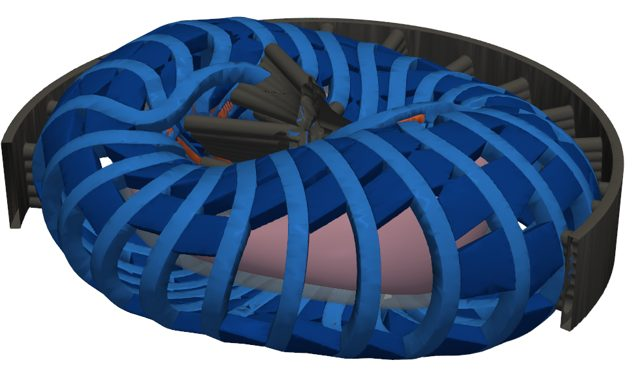
\includegraphics[width=\linewidth]{bilder/katalog/0000.jpg}\par\scriptsize \begin{tabular}{@{}l@{\,}r@{\quad}l@{\,}r@{}}Spulen & 24 & $\sigma_{99}$ & \num{840} MPa \\Verb./Paar & 10 & max. & \num{3425} MPa \\$E_V$ & \num{70} GPa & Dehnung & \num{0.42} \% \\Abstand & \num{0.18} & $B\cdot n$ & \num{1.98} ‰ \\Stahl & \num{23} kt & frei & \num{1.44} m \\\end{tabular}\par verletzt: Stahl σ99, Dehnung Wickelpaket. PicoGK: keine Überschneidung.\end{minipage}\hfill
\begin{minipage}[t]{0.47\linewidth}\textbf{0001} \hfill \num{-191}\,\%\par 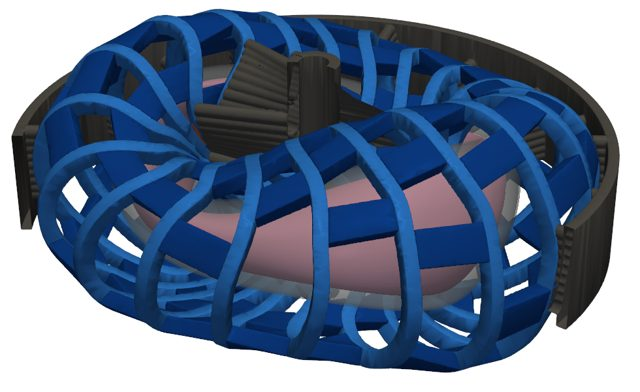
\includegraphics[width=\linewidth]{bilder/katalog/0001.jpg}\par\scriptsize \begin{tabular}{@{}l@{\,}r@{\quad}l@{\,}r@{}}Spulen & 20 & $\sigma_{99}$ & \num{1456} MPa \\Verb./Paar & 7 & max. & \num{3851} MPa \\$E_V$ & \num{135} GPa & Dehnung & \num{0.60} \% \\Abstand & \num{0.24} & $B\cdot n$ & \num{1.53} ‰ \\Stahl & \num{12} kt & frei & \num{2.00} m \\\end{tabular}\par verletzt: Stahl σ99, Dehnung Wickelpaket. PicoGK: keine Überschneidung.\end{minipage}\par\vspace{6pt}
\begin{minipage}[t]{0.47\linewidth}\textbf{0002} \hfill \num{-844}\,\%\par 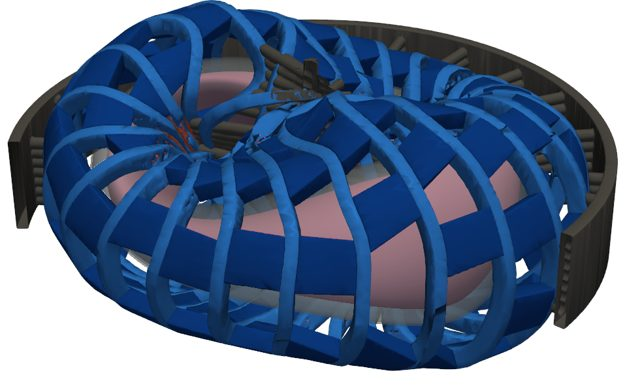
\includegraphics[width=\linewidth]{bilder/katalog/0002.jpg}\par\scriptsize \begin{tabular}{@{}l@{\,}r@{\quad}l@{\,}r@{}}Spulen & 24 & $\sigma_{99}$ & \num{4721} MPa \\Verb./Paar & 8 & max. & \num{13357} MPa \\$E_V$ & \num{25} GPa & Dehnung & \num{2.01} \% \\Abstand & \num{0.30} & $B\cdot n$ & \num{3.67} ‰ \\Stahl & \num{13} kt & frei & \num{2.39} m \\\end{tabular}\par verletzt: Stahl σ99, Dehnung Wickelpaket, Feldfehler B·n. PicoGK: keine Überschneidung.\end{minipage}\hfill
\begin{minipage}[t]{0.47\linewidth}\textbf{0003} \hfill \num{-216}\,\%\par 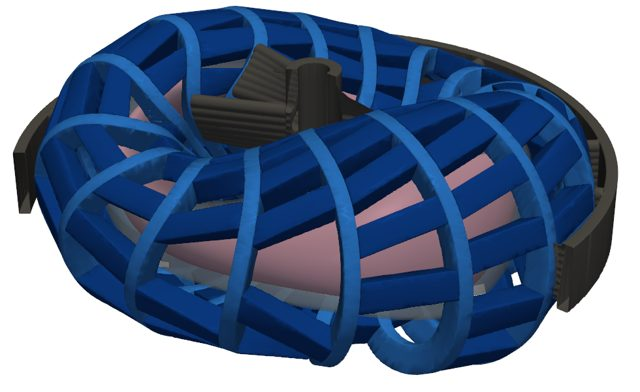
\includegraphics[width=\linewidth]{bilder/katalog/0003.jpg}\par\scriptsize \begin{tabular}{@{}l@{\,}r@{\quad}l@{\,}r@{}}Spulen & 16 & $\sigma_{99}$ & \num{617} MPa \\Verb./Paar & 12 & max. & \num{1361} MPa \\$E_V$ & \num{142} GPa & Dehnung & \num{0.26} \% \\Abstand & \num{0.20} & $B\cdot n$ & \num{9.48} ‰ \\Stahl & \num{20} kt & frei & \num{1.40} m \\\end{tabular}\par verletzt: Stahl σ99, Feldfehler B·n. PicoGK: keine Überschneidung.\end{minipage}\par\vspace{6pt}
\clearpage
\begin{minipage}[t]{0.47\linewidth}\textbf{0004} \hfill \num{-12}\,\%\par 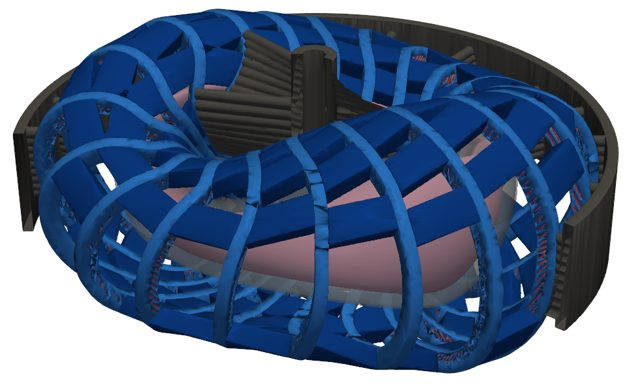
\includegraphics[width=\linewidth]{bilder/katalog/0004.jpg}\par\scriptsize \begin{tabular}{@{}l@{\,}r@{\quad}l@{\,}r@{}}Spulen & 20 & $\sigma_{99}$ & \num{558} MPa \\Verb./Paar & 10 & max. & \num{1085} MPa \\$E_V$ & \num{148} GPa & Dehnung & \num{0.26} \% \\Abstand & \num{0.19} & $B\cdot n$ & \num{1.81} ‰ \\Stahl & \num{19} kt & frei & \num{1.54} m \\\end{tabular}\par verletzt: Stahl σ99. PicoGK: keine Überschneidung.\end{minipage}\hfill
\begin{minipage}[t]{0.47\linewidth}\textbf{0005} \hfill \num{-69}\,\%\par 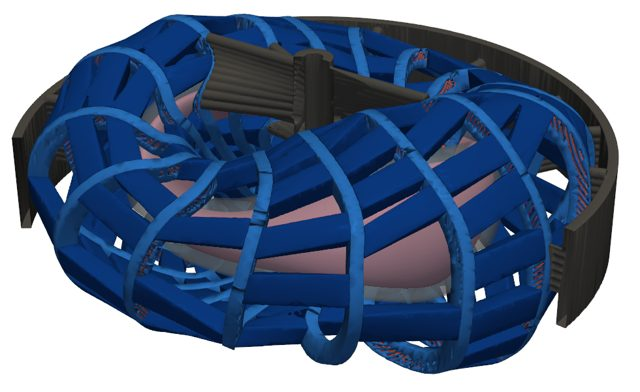
\includegraphics[width=\linewidth]{bilder/katalog/0005.jpg}\par\scriptsize \begin{tabular}{@{}l@{\,}r@{\quad}l@{\,}r@{}}Spulen & 16 & $\sigma_{99}$ & \num{844} MPa \\Verb./Paar & 13 & max. & \num{1847} MPa \\$E_V$ & \num{114} GPa & Dehnung & \num{0.35} \% \\Abstand & \num{0.15} & $B\cdot n$ & \num{2.40} ‰ \\Stahl & \num{23} kt & frei & \num{1.26} m \\\end{tabular}\par verletzt: Stahl σ99, Dehnung Wickelpaket, Neutronenfluenz. PicoGK: keine Überschneidung.\end{minipage}\par\vspace{6pt}
\begin{minipage}[t]{0.47\linewidth}\textbf{0006} \hfill \num{-1480}\,\%\par 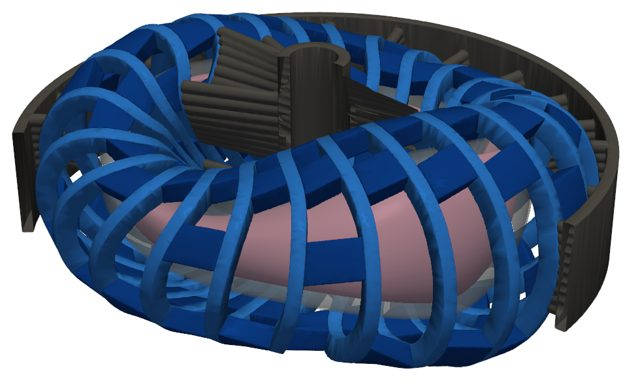
\includegraphics[width=\linewidth]{bilder/katalog/0006.jpg}\par\scriptsize \begin{tabular}{@{}l@{\,}r@{\quad}l@{\,}r@{}}Spulen & 24 & $\sigma_{99}$ & \num{536} MPa \\Verb./Paar & 6 & max. & \num{1222} MPa \\$E_V$ & \num{78} GPa & Dehnung & \num{0.22} \% \\Abstand & \num{0.12} & $B\cdot n$ & \num{1.77} ‰ \\Stahl & \num{14} kt & frei & \num{0.99} m \\\end{tabular}\par verletzt: Stahl σ99, Platz Package, Kernheizung, Neutronenfluenz. PicoGK: keine Überschneidung.\end{minipage}\hfill
\begin{minipage}[t]{0.47\linewidth}\textbf{0007} \hfill \num{-231}\,\%\par 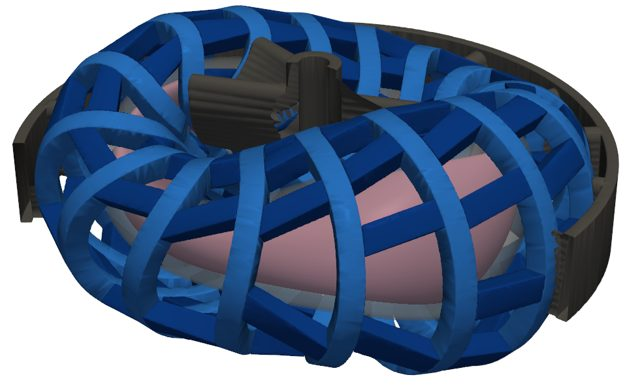
\includegraphics[width=\linewidth]{bilder/katalog/0007.jpg}\par\scriptsize \begin{tabular}{@{}l@{\,}r@{\quad}l@{\,}r@{}}Spulen & 16 & $\sigma_{99}$ & \num{870} MPa \\Verb./Paar & 8 & max. & \num{3574} MPa \\$E_V$ & \num{88} GPa & Dehnung & \num{0.42} \% \\Abstand & \num{0.16} & $B\cdot n$ & \num{9.92} ‰ \\Stahl & \num{17} kt & frei & \num{1.60} m \\\end{tabular}\par verletzt: Stahl σ99, Dehnung Wickelpaket, Feldfehler B·n. PicoGK: keine Überschneidung.\end{minipage}\par\vspace{6pt}
\clearpage
\begin{minipage}[t]{0.47\linewidth}\textbf{0008} \hfill \num{27}\,\%\par 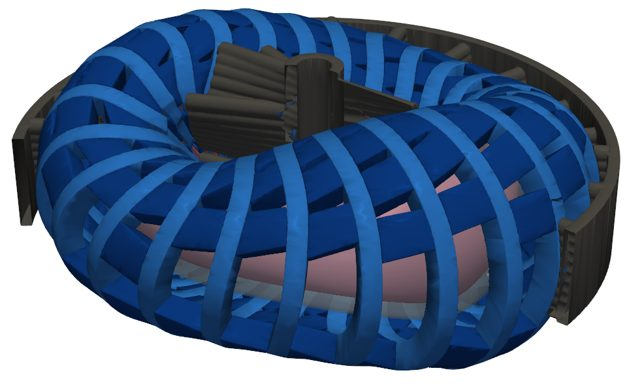
\includegraphics[width=\linewidth]{bilder/katalog/0008.jpg}\par\scriptsize \begin{tabular}{@{}l@{\,}r@{\quad}l@{\,}r@{}}Spulen & 24 & $\sigma_{99}$ & \num{305} MPa \\Verb./Paar & 11 & max. & \num{1695} MPa \\$E_V$ & \num{142} GPa & Dehnung & \num{0.17} \% \\Abstand & \num{0.21} & $B\cdot n$ & \num{2.20} ‰ \\Stahl & \num{26} kt & frei & \num{1.48} m \\\end{tabular}\par \textbf{zulässig}. PicoGK: keine Überschneidung.\end{minipage}\hfill
\begin{minipage}[t]{0.47\linewidth}\textbf{0009} \hfill \num{-132}\,\%\par 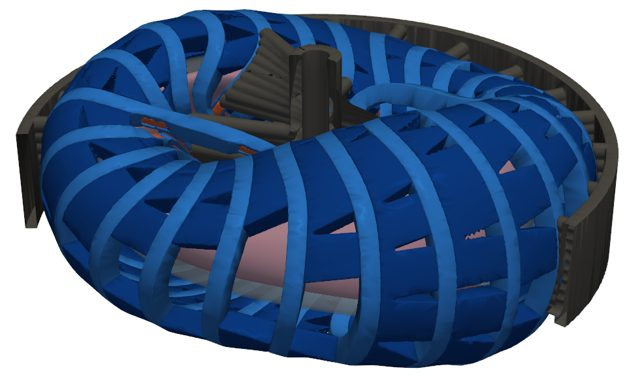
\includegraphics[width=\linewidth]{bilder/katalog/0009.jpg}\par\scriptsize \begin{tabular}{@{}l@{\,}r@{\quad}l@{\,}r@{}}Spulen & 24 & $\sigma_{99}$ & \num{1159} MPa \\Verb./Paar & 13 & max. & \num{9216} MPa \\$E_V$ & \num{145} GPa & Dehnung & \num{0.62} \% \\Abstand & \num{0.23} & $B\cdot n$ & \num{1.50} ‰ \\Stahl & \num{24} kt & frei & \num{1.55} m \\\end{tabular}\par verletzt: Stahl σ99, Dehnung Wickelpaket. PicoGK: keine Überschneidung.\end{minipage}\par\vspace{6pt}
\begin{minipage}[t]{0.47\linewidth}\textbf{0010} \hfill \num{-176}\,\%\par 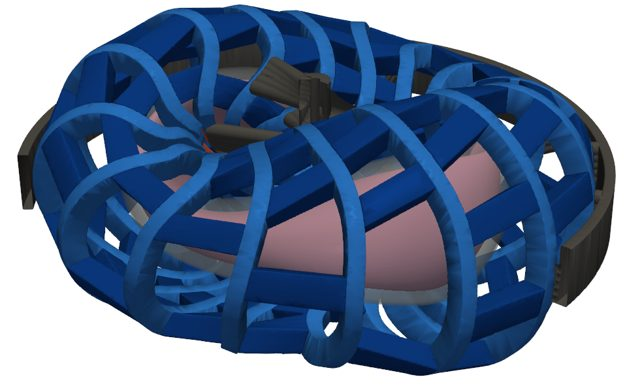
\includegraphics[width=\linewidth]{bilder/katalog/0010.jpg}\par\scriptsize \begin{tabular}{@{}l@{\,}r@{\quad}l@{\,}r@{}}Spulen & 16 & $\sigma_{99}$ & \num{1381} MPa \\Verb./Paar & 8 & max. & \num{8739} MPa \\$E_V$ & \num{149} GPa & Dehnung & \num{0.63} \% \\Abstand & \num{0.27} & $B\cdot n$ & \num{2.80} ‰ \\Stahl & \num{21} kt & frei & \num{1.93} m \\\end{tabular}\par verletzt: Stahl σ99, Dehnung Wickelpaket. PicoGK: keine Überschneidung.\end{minipage}\hfill
\begin{minipage}[t]{0.47\linewidth}\textbf{0011} \hfill \num{-519}\,\%\par 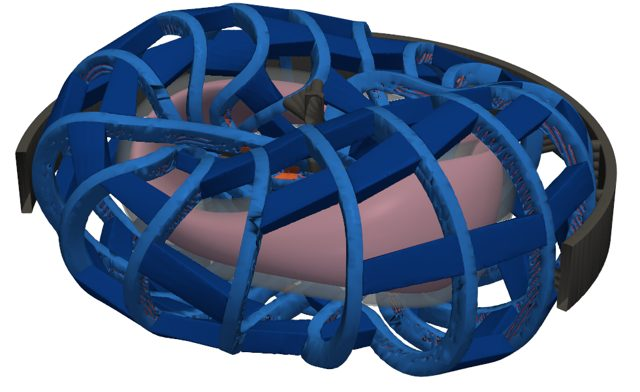
\includegraphics[width=\linewidth]{bilder/katalog/0011.jpg}\par\scriptsize \begin{tabular}{@{}l@{\,}r@{\quad}l@{\,}r@{}}Spulen & 16 & $\sigma_{99}$ & \num{3096} MPa \\Verb./Paar & 7 & max. & \num{19166} MPa \\$E_V$ & \num{42} GPa & Dehnung & \num{1.50} \% \\Abstand & \num{0.18} & $B\cdot n$ & \num{3.25} ‰ \\Stahl & \num{14} kt & frei & \num{1.80} m \\\end{tabular}\par verletzt: Stahl σ99, Dehnung Wickelpaket, Feldfehler B·n. PicoGK: keine Überschneidung.\end{minipage}\par\vspace{6pt}
\clearpage
\begin{minipage}[t]{0.47\linewidth}\textbf{0012} \hfill \num{-139}\,\%\par 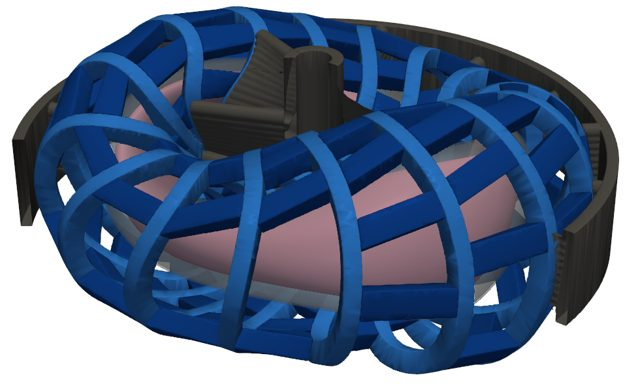
\includegraphics[width=\linewidth]{bilder/katalog/0012.jpg}\par\scriptsize \begin{tabular}{@{}l@{\,}r@{\quad}l@{\,}r@{}}Spulen & 16 & $\sigma_{99}$ & \num{999} MPa \\Verb./Paar & 9 & max. & \num{2952} MPa \\$E_V$ & \num{50} GPa & Dehnung & \num{0.40} \% \\Abstand & \num{0.21} & $B\cdot n$ & \num{7.17} ‰ \\Stahl & \num{13} kt & frei & \num{1.68} m \\\end{tabular}\par verletzt: Stahl σ99, Dehnung Wickelpaket, Feldfehler B·n. PicoGK: keine Überschneidung.\end{minipage}\hfill
\begin{minipage}[t]{0.47\linewidth}\textbf{0013} \hfill \num{-55}\,\%\par 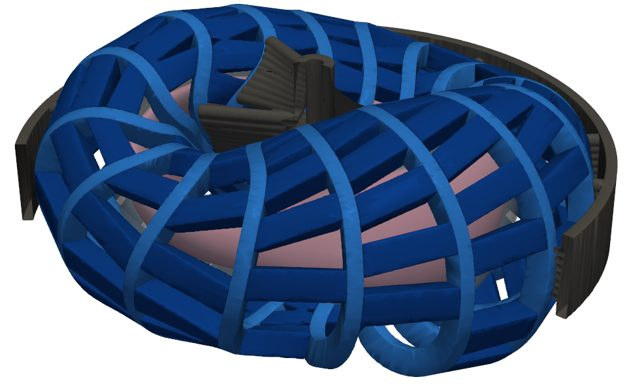
\includegraphics[width=\linewidth]{bilder/katalog/0013.jpg}\par\scriptsize \begin{tabular}{@{}l@{\,}r@{\quad}l@{\,}r@{}}Spulen & 16 & $\sigma_{99}$ & \num{773} MPa \\Verb./Paar & 14 & max. & \num{1718} MPa \\$E_V$ & \num{103} GPa & Dehnung & \num{0.34} \% \\Abstand & \num{0.13} & $B\cdot n$ & \num{4.32} ‰ \\Stahl & \num{25} kt & frei & \num{1.63} m \\\end{tabular}\par verletzt: Stahl σ99, Dehnung Wickelpaket, Feldfehler B·n. PicoGK: keine Überschneidung.\end{minipage}\par\vspace{6pt}
\begin{minipage}[t]{0.47\linewidth}\textbf{0014} \hfill \num{25}\,\%\par 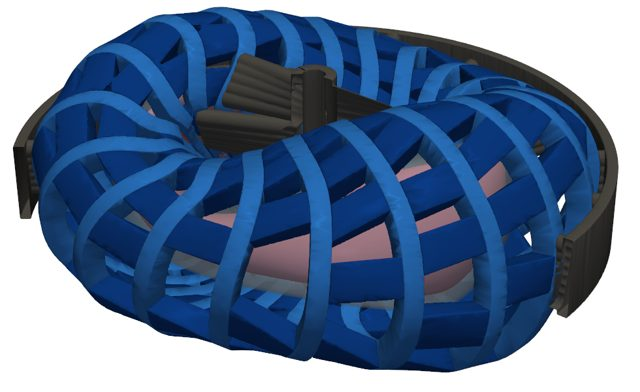
\includegraphics[width=\linewidth]{bilder/katalog/0014.jpg}\par\scriptsize \begin{tabular}{@{}l@{\,}r@{\quad}l@{\,}r@{}}Spulen & 20 & $\sigma_{99}$ & \num{377} MPa \\Verb./Paar & 11 & max. & \num{1419} MPa \\$E_V$ & \num{196} GPa & Dehnung & \num{0.21} \% \\Abstand & \num{0.23} & $B\cdot n$ & \num{2.21} ‰ \\Stahl & \num{28} kt & frei & \num{1.65} m \\\end{tabular}\par \textbf{zulässig}. PicoGK: keine Überschneidung.\end{minipage}\hfill
\begin{minipage}[t]{0.47\linewidth}\textbf{0015} \hfill \num{-628}\,\%\par 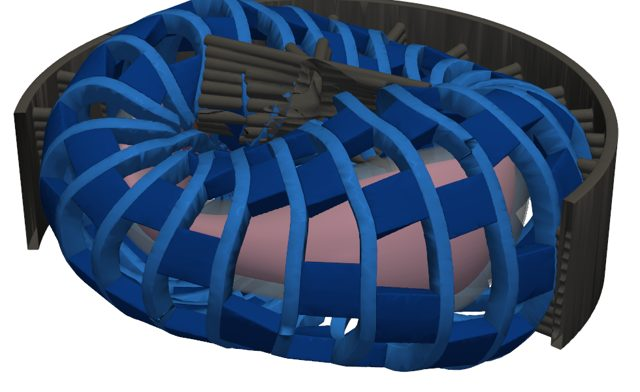
\includegraphics[width=\linewidth]{bilder/katalog/0015.jpg}\par\scriptsize \begin{tabular}{@{}l@{\,}r@{\quad}l@{\,}r@{}}Spulen & 24 & $\sigma_{99}$ & \num{3586} MPa \\Verb./Paar & 7 & max. & \num{30683} MPa \\$E_V$ & \num{168} GPa & Dehnung & \num{2.18} \% \\Abstand & \num{0.29} & $B\cdot n$ & \num{1.12} ‰ \\Stahl & \num{18} kt & frei & \num{2.48} m \\\end{tabular}\par verletzt: Stahl σ99, Dehnung Wickelpaket. PicoGK: keine Überschneidung.\end{minipage}\par\vspace{6pt}
\clearpage
\begin{minipage}[t]{0.47\linewidth}\textbf{0016} \hfill \num{-600}\,\%\par 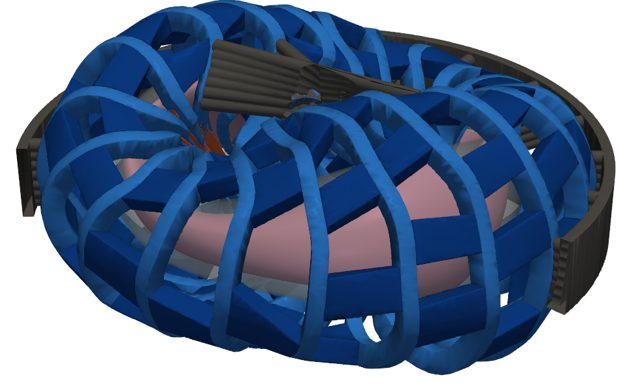
\includegraphics[width=\linewidth]{bilder/katalog/0016.jpg}\par\scriptsize \begin{tabular}{@{}l@{\,}r@{\quad}l@{\,}r@{}}Spulen & 20 & $\sigma_{99}$ & \num{3499} MPa \\Verb./Paar & 8 & max. & \num{15129} MPa \\$E_V$ & \num{172} GPa & Dehnung & \num{1.95} \% \\Abstand & \num{0.29} & $B\cdot n$ & \num{2.24} ‰ \\Stahl & \num{19} kt & frei & \num{2.42} m \\\end{tabular}\par verletzt: Stahl σ99, Dehnung Wickelpaket. PicoGK: keine Überschneidung.\end{minipage}\hfill
\begin{minipage}[t]{0.47\linewidth}\textbf{0017} \hfill \num{20}\,\%\par 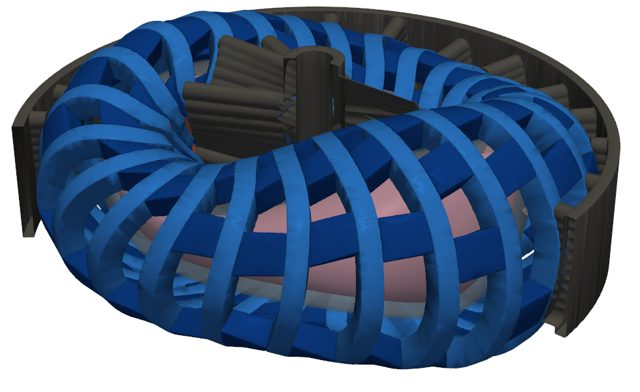
\includegraphics[width=\linewidth]{bilder/katalog/0017.jpg}\par\scriptsize \begin{tabular}{@{}l@{\,}r@{\quad}l@{\,}r@{}}Spulen & 24 & $\sigma_{99}$ & \num{389} MPa \\Verb./Paar & 7 & max. & \num{1721} MPa \\$E_V$ & \num{29} GPa & Dehnung & \num{0.20} \% \\Abstand & \num{0.22} & $B\cdot n$ & \num{1.66} ‰ \\Stahl & \num{23} kt & frei & \num{1.30} m \\\end{tabular}\par \textbf{zulässig}. PicoGK: keine Überschneidung.\end{minipage}\par\vspace{6pt}
\begin{minipage}[t]{0.47\linewidth}\textbf{0018}$^\ast$ \hfill \num{-99}\,\%\par 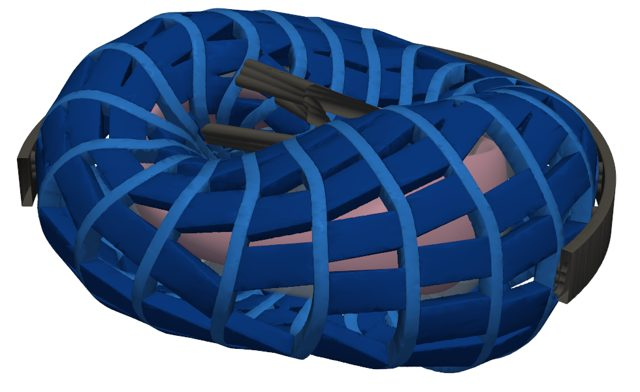
\includegraphics[width=\linewidth]{bilder/katalog/0018.jpg}\par\scriptsize \begin{tabular}{@{}l@{\,}r@{\quad}l@{\,}r@{}}Spulen & 20 & $\sigma_{99}$ & \num{996} MPa \\Verb./Paar & 14 & max. & \num{4566} MPa \\$E_V$ & \num{26} GPa & Dehnung & \num{0.44} \% \\Abstand & \num{0.25} & $B\cdot n$ & \num{1.43} ‰ \\Stahl & \num{24} kt & frei & \num{2.08} m \\\end{tabular}\par verletzt: Stahl σ99, Dehnung Wickelpaket. PicoGK: keine Überschneidung.\end{minipage}\hfill
\begin{minipage}[t]{0.47\linewidth}\textbf{0019} \hfill \num{-338}\,\%\par 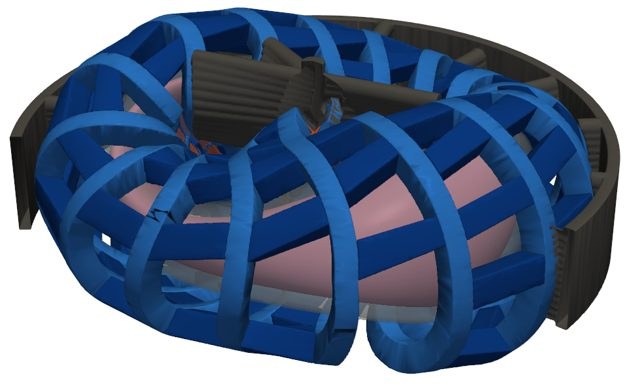
\includegraphics[width=\linewidth]{bilder/katalog/0019.jpg}\par\scriptsize \begin{tabular}{@{}l@{\,}r@{\quad}l@{\,}r@{}}Spulen & 16 & $\sigma_{99}$ & \num{1571} MPa \\Verb./Paar & 9 & max. & \num{14989} MPa \\$E_V$ & \num{24} GPa & Dehnung & \num{0.96} \% \\Abstand & \num{0.25} & $B\cdot n$ & \num{13.15} ‰ \\Stahl & \num{17} kt & frei & \num{1.93} m \\\end{tabular}\par verletzt: Stahl σ99, Dehnung Wickelpaket, Feldfehler B·n. PicoGK: keine Überschneidung.\end{minipage}\par\vspace{6pt}
\clearpage
\begin{minipage}[t]{0.47\linewidth}\textbf{0020} \hfill \num{-173}\,\%\par 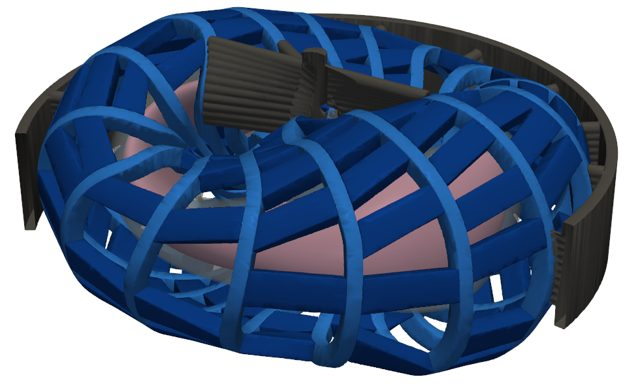
\includegraphics[width=\linewidth]{bilder/katalog/0020.jpg}\par\scriptsize \begin{tabular}{@{}l@{\,}r@{\quad}l@{\,}r@{}}Spulen & 16 & $\sigma_{99}$ & \num{1363} MPa \\Verb./Paar & 14 & max. & \num{6952} MPa \\$E_V$ & \num{137} GPa & Dehnung & \num{0.55} \% \\Abstand & \num{0.24} & $B\cdot n$ & \num{3.21} ‰ \\Stahl & \num{17} kt & frei & \num{1.78} m \\\end{tabular}\par verletzt: Stahl σ99, Dehnung Wickelpaket, Feldfehler B·n. PicoGK: keine Überschneidung.\end{minipage}\hfill
\begin{minipage}[t]{0.47\linewidth}\textbf{0021} \hfill \num{-4948}\,\%\par 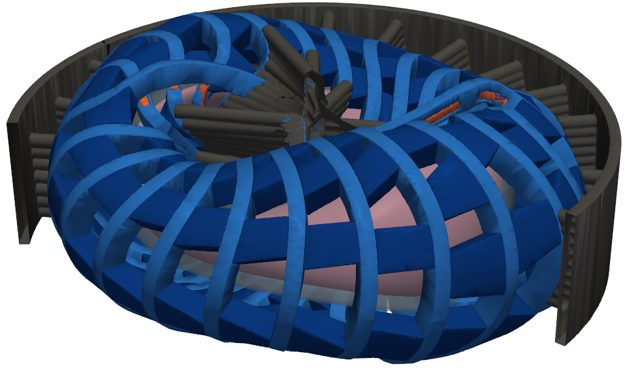
\includegraphics[width=\linewidth]{bilder/katalog/0021.jpg}\par\scriptsize \begin{tabular}{@{}l@{\,}r@{\quad}l@{\,}r@{}}Spulen & 24 & $\sigma_{99}$ & \num{558} MPa \\Verb./Paar & 8 & max. & \num{4173} MPa \\$E_V$ & \num{138} GPa & Dehnung & \num{0.29} \% \\Abstand & \num{0.16} & $B\cdot n$ & \num{2.26} ‰ \\Stahl & \num{26} kt & frei & \num{0.87} m \\\end{tabular}\par verletzt: Stahl σ99, Platz Package, Kernheizung, Neutronenfluenz. PicoGK: Überschneidung!\end{minipage}\par\vspace{6pt}
\begin{minipage}[t]{0.47\linewidth}\textbf{0022} \hfill \num{-20}\,\%\par 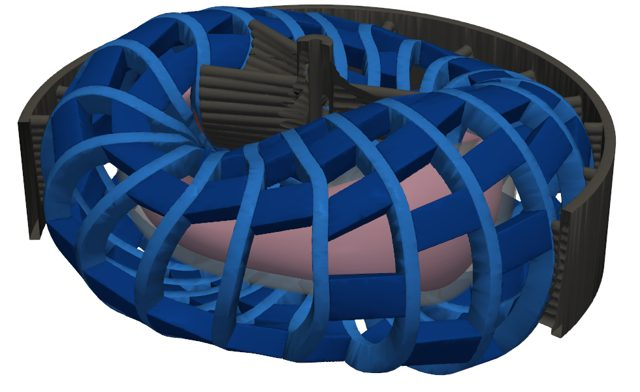
\includegraphics[width=\linewidth]{bilder/katalog/0022.jpg}\par\scriptsize \begin{tabular}{@{}l@{\,}r@{\quad}l@{\,}r@{}}Spulen & 20 & $\sigma_{99}$ & \num{600} MPa \\Verb./Paar & 8 & max. & \num{2183} MPa \\$E_V$ & \num{37} GPa & Dehnung & \num{0.26} \% \\Abstand & \num{0.23} & $B\cdot n$ & \num{0.70} ‰ \\Stahl & \num{24} kt & frei & \num{1.57} m \\\end{tabular}\par verletzt: Stahl σ99. PicoGK: keine Überschneidung.\end{minipage}\hfill
\begin{minipage}[t]{0.47\linewidth}\textbf{0023} \hfill \num{-276}\,\%\par 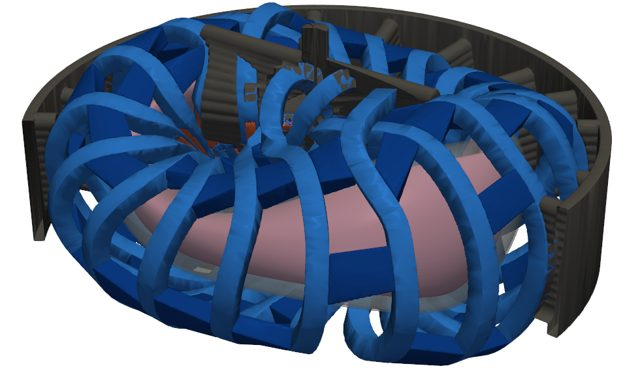
\includegraphics[width=\linewidth]{bilder/katalog/0023.jpg}\par\scriptsize \begin{tabular}{@{}l@{\,}r@{\quad}l@{\,}r@{}}Spulen & 20 & $\sigma_{99}$ & \num{1864} MPa \\Verb./Paar & 6 & max. & \num{10858} MPa \\$E_V$ & \num{156} GPa & Dehnung & \num{1.13} \% \\Abstand & \num{0.28} & $B\cdot n$ & \num{2.89} ‰ \\Stahl & \num{15} kt & frei & \num{2.06} m \\\end{tabular}\par verletzt: Stahl σ99, Dehnung Wickelpaket. PicoGK: keine Überschneidung.\end{minipage}\par\vspace{6pt}
\clearpage
\begin{minipage}[t]{0.47\linewidth}\textbf{0024} \hfill \num{-257}\,\%\par 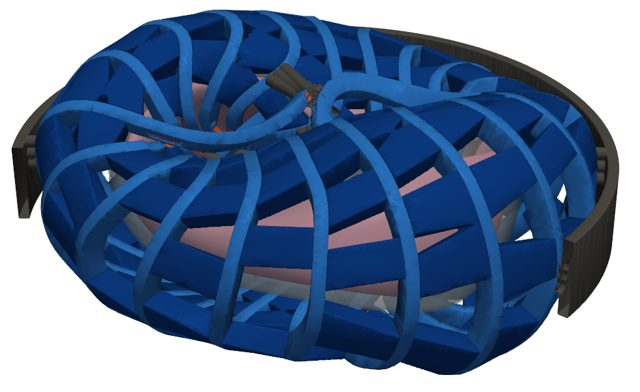
\includegraphics[width=\linewidth]{bilder/katalog/0024.jpg}\par\scriptsize \begin{tabular}{@{}l@{\,}r@{\quad}l@{\,}r@{}}Spulen & 20 & $\sigma_{99}$ & \num{1787} MPa \\Verb./Paar & 11 & max. & \num{7614} MPa \\$E_V$ & \num{24} GPa & Dehnung & \num{0.85} \% \\Abstand & \num{0.26} & $B\cdot n$ & \num{1.55} ‰ \\Stahl & \num{24} kt & frei & \num{1.82} m \\\end{tabular}\par verletzt: Stahl σ99, Dehnung Wickelpaket. PicoGK: keine Überschneidung.\end{minipage}\hfill
\begin{minipage}[t]{0.47\linewidth}\textbf{0025} \hfill \num{-102}\,\%\par 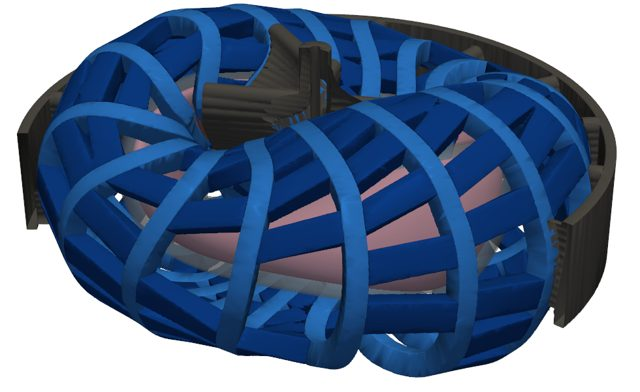
\includegraphics[width=\linewidth]{bilder/katalog/0025.jpg}\par\scriptsize \begin{tabular}{@{}l@{\,}r@{\quad}l@{\,}r@{}}Spulen & 16 & $\sigma_{99}$ & \num{1010} MPa \\Verb./Paar & 14 & max. & \num{9842} MPa \\$E_V$ & \num{41} GPa & Dehnung & \num{0.50} \% \\Abstand & \num{0.18} & $B\cdot n$ & \num{1.94} ‰ \\Stahl & \num{26} kt & frei & \num{1.88} m \\\end{tabular}\par verletzt: Stahl σ99, Dehnung Wickelpaket. PicoGK: keine Überschneidung.\end{minipage}\par\vspace{6pt}
\begin{minipage}[t]{0.47\linewidth}\textbf{0026} \hfill \num{-62}\,\%\par 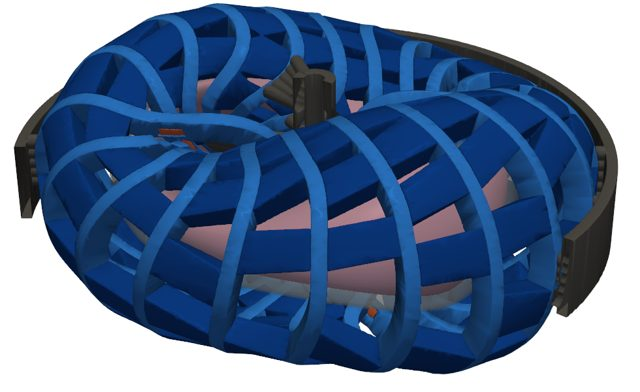
\includegraphics[width=\linewidth]{bilder/katalog/0026.jpg}\par\scriptsize \begin{tabular}{@{}l@{\,}r@{\quad}l@{\,}r@{}}Spulen & 20 & $\sigma_{99}$ & \num{809} MPa \\Verb./Paar & 11 & max. & \num{2253} MPa \\$E_V$ & \num{79} GPa & Dehnung & \num{0.38} \% \\Abstand & \num{0.19} & $B\cdot n$ & \num{1.43} ‰ \\Stahl & \num{29} kt & frei & \num{1.41} m \\\end{tabular}\par verletzt: Stahl σ99, Dehnung Wickelpaket. PicoGK: keine Überschneidung.\end{minipage}\hfill
\begin{minipage}[t]{0.47\linewidth}\textbf{0027} \hfill \num{-316}\,\%\par 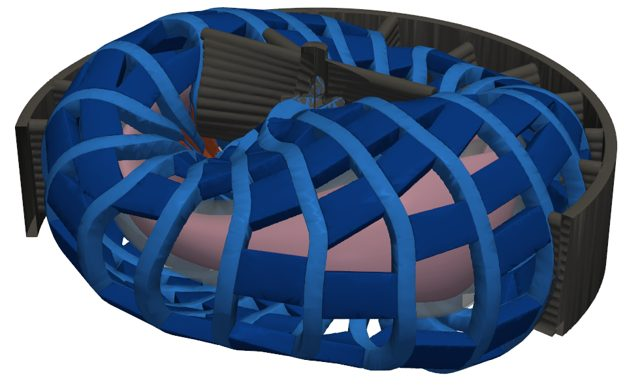
\includegraphics[width=\linewidth]{bilder/katalog/0027.jpg}\par\scriptsize \begin{tabular}{@{}l@{\,}r@{\quad}l@{\,}r@{}}Spulen & 20 & $\sigma_{99}$ & \num{2080} MPa \\Verb./Paar & 10 & max. & \num{10143} MPa \\$E_V$ & \num{171} GPa & Dehnung & \num{1.02} \% \\Abstand & \num{0.28} & $B\cdot n$ & \num{2.25} ‰ \\Stahl & \num{16} kt & frei & \num{2.18} m \\\end{tabular}\par verletzt: Stahl σ99, Dehnung Wickelpaket. PicoGK: keine Überschneidung.\end{minipage}\par\vspace{6pt}
\clearpage
\begin{minipage}[t]{0.47\linewidth}\textbf{0028} \hfill \num{-78}\,\%\par 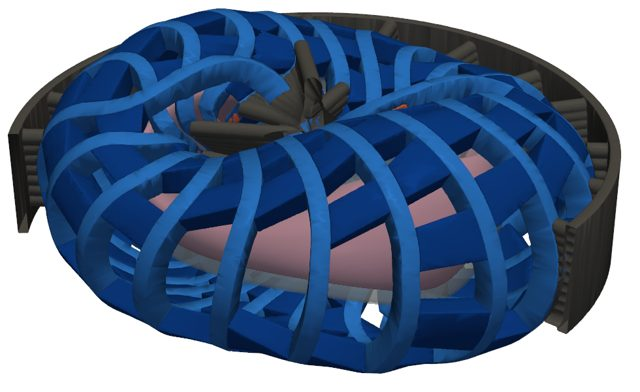
\includegraphics[width=\linewidth]{bilder/katalog/0028.jpg}\par\scriptsize \begin{tabular}{@{}l@{\,}r@{\quad}l@{\,}r@{}}Spulen & 20 & $\sigma_{99}$ & \num{888} MPa \\Verb./Paar & 9 & max. & \num{3682} MPa \\$E_V$ & \num{22} GPa & Dehnung & \num{0.40} \% \\Abstand & \num{0.17} & $B\cdot n$ & \num{1.45} ‰ \\Stahl & \num{30} kt & frei & \num{1.33} m \\\end{tabular}\par verletzt: Stahl σ99, Dehnung Wickelpaket. PicoGK: keine Überschneidung.\end{minipage}\hfill
\begin{minipage}[t]{0.47\linewidth}\textbf{0029} \hfill \num{-361}\,\%\par 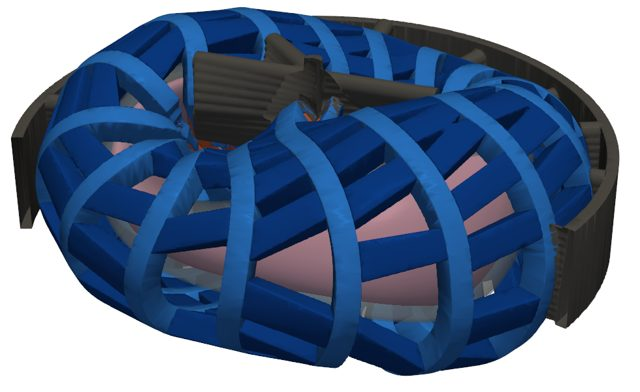
\includegraphics[width=\linewidth]{bilder/katalog/0029.jpg}\par\scriptsize \begin{tabular}{@{}l@{\,}r@{\quad}l@{\,}r@{}}Spulen & 16 & $\sigma_{99}$ & \num{1975} MPa \\Verb./Paar & 13 & max. & \num{34584} MPa \\$E_V$ & \num{27} GPa & Dehnung & \num{1.38} \% \\Abstand & \num{0.29} & $B\cdot n$ & \num{10.34} ‰ \\Stahl & \num{22} kt & frei & \num{2.35} m \\\end{tabular}\par verletzt: Stahl σ99, Dehnung Wickelpaket, Feldfehler B·n. PicoGK: keine Überschneidung.\end{minipage}\par\vspace{6pt}
\begin{minipage}[t]{0.47\linewidth}\textbf{0031} \hfill \num{-222}\,\%\par 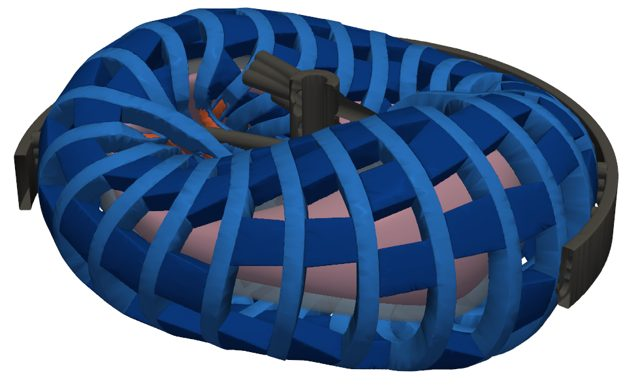
\includegraphics[width=\linewidth]{bilder/katalog/0031.jpg}\par\scriptsize \begin{tabular}{@{}l@{\,}r@{\quad}l@{\,}r@{}}Spulen & 24 & $\sigma_{99}$ & \num{1514} MPa \\Verb./Paar & 8 & max. & \num{8426} MPa \\$E_V$ & \num{190} GPa & Dehnung & \num{0.97} \% \\Abstand & \num{0.24} & $B\cdot n$ & \num{1.99} ‰ \\Stahl & \num{21} kt & frei & \num{1.84} m \\\end{tabular}\par verletzt: Stahl σ99, Dehnung Wickelpaket. PicoGK: keine Überschneidung.\end{minipage}\hfill
\begin{minipage}[t]{0.47\linewidth}\textbf{0032} \hfill \num{-123}\,\%\par 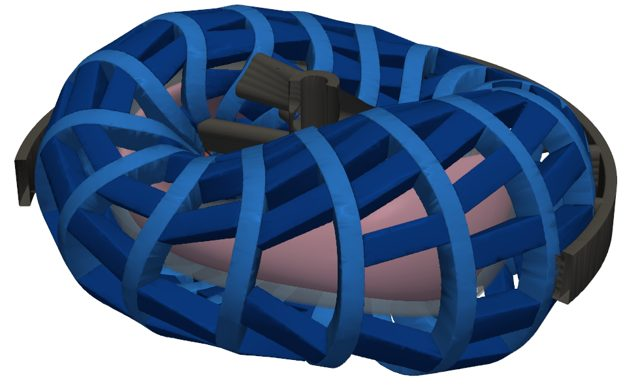
\includegraphics[width=\linewidth]{bilder/katalog/0032.jpg}\par\scriptsize \begin{tabular}{@{}l@{\,}r@{\quad}l@{\,}r@{}}Spulen & 16 & $\sigma_{99}$ & \num{777} MPa \\Verb./Paar & 12 & max. & \num{3008} MPa \\$E_V$ & \num{38} GPa & Dehnung & \num{0.28} \% \\Abstand & \num{0.17} & $B\cdot n$ & \num{6.70} ‰ \\Stahl & \num{25} kt & frei & \num{1.48} m \\\end{tabular}\par verletzt: Stahl σ99, Feldfehler B·n. PicoGK: keine Überschneidung.\end{minipage}\par\vspace{6pt}
\clearpage
\begin{minipage}[t]{0.47\linewidth}\textbf{0033} \hfill \num{-125}\,\%\par 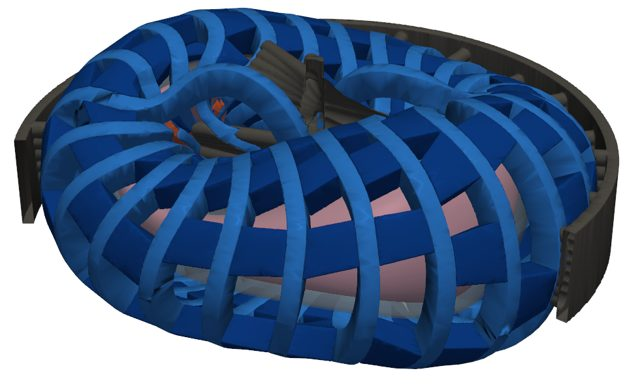
\includegraphics[width=\linewidth]{bilder/katalog/0033.jpg}\par\scriptsize \begin{tabular}{@{}l@{\,}r@{\quad}l@{\,}r@{}}Spulen & 24 & $\sigma_{99}$ & \num{1019} MPa \\Verb./Paar & 8 & max. & \num{4409} MPa \\$E_V$ & \num{118} GPa & Dehnung & \num{0.68} \% \\Abstand & \num{0.25} & $B\cdot n$ & \num{1.78} ‰ \\Stahl & \num{25} kt & frei & \num{1.56} m \\\end{tabular}\par verletzt: Stahl σ99, Dehnung Wickelpaket. PicoGK: keine Überschneidung.\end{minipage}\hfill
\begin{minipage}[t]{0.47\linewidth}\textbf{0034} \hfill \num{-215}\,\%\par \par\scriptsize \begin{tabular}{@{}l@{\,}r@{\quad}l@{\,}r@{}}Spulen & 16 & $\sigma_{99}$ & \num{1574} MPa \\Verb./Paar & 6 & max. & \num{4775} MPa \\$E_V$ & \num{21} GPa & Dehnung & \num{0.56} \% \\Abstand & \num{0.26} & $B\cdot n$ & \num{3.08} ‰ \\Stahl & \num{17} kt & frei & \num{1.96} m \\\end{tabular}\par verletzt: Stahl σ99, Dehnung Wickelpaket, Feldfehler B·n.\end{minipage}\par\vspace{6pt}
\begin{minipage}[t]{0.47\linewidth}\textbf{0035} \hfill \num{-278}\,\%\par \par\scriptsize \begin{tabular}{@{}l@{\,}r@{\quad}l@{\,}r@{}}Spulen & 24 & $\sigma_{99}$ & \num{1892} MPa \\Verb./Paar & 12 & max. & \num{5956} MPa \\$E_V$ & \num{50} GPa & Dehnung & \num{0.83} \% \\Abstand & \num{0.18} & $B\cdot n$ & \num{1.23} ‰ \\Stahl & \num{30} kt & frei & \num{1.31} m \\\end{tabular}\par verletzt: Stahl σ99, Dehnung Wickelpaket.\end{minipage}\hfill
\begin{minipage}[t]{0.47\linewidth}\textbf{0036} \hfill \num{-37}\,\%\par \par\scriptsize \begin{tabular}{@{}l@{\,}r@{\quad}l@{\,}r@{}}Spulen & 20 & $\sigma_{99}$ & \num{683} MPa \\Verb./Paar & 7 & max. & \num{7457} MPa \\$E_V$ & \num{119} GPa & Dehnung & \num{0.38} \% \\Abstand & \num{0.25} & $B\cdot n$ & \num{3.45} ‰ \\Stahl & \num{15} kt & frei & \num{1.74} m \\\end{tabular}\par verletzt: Stahl σ99, Dehnung Wickelpaket, Feldfehler B·n.\end{minipage}\par\vspace{6pt}
\clearpage
\begin{minipage}[t]{0.47\linewidth}\textbf{0037} \hfill \num{-260}\,\%\par \par\scriptsize \begin{tabular}{@{}l@{\,}r@{\quad}l@{\,}r@{}}Spulen & 24 & $\sigma_{99}$ & \num{1800} MPa \\Verb./Paar & 6 & max. & \num{4950} MPa \\$E_V$ & \num{53} GPa & Dehnung & \num{0.66} \% \\Abstand & \num{0.13} & $B\cdot n$ & \num{1.33} ‰ \\Stahl & \num{12} kt & frei & \num{1.43} m \\\end{tabular}\par verletzt: Stahl σ99, Dehnung Wickelpaket.\end{minipage}\hfill
\begin{minipage}[t]{0.47\linewidth}\textbf{0038} \hfill \num{-204}\,\%\par \par\scriptsize \begin{tabular}{@{}l@{\,}r@{\quad}l@{\,}r@{}}Spulen & 20 & $\sigma_{99}$ & \num{525} MPa \\Verb./Paar & 13 & max. & \num{2561} MPa \\$E_V$ & \num{60} GPa & Dehnung & \num{0.23} \% \\Abstand & \num{0.17} & $B\cdot n$ & \num{3.27} ‰ \\Stahl & \num{32} kt & frei & \num{1.15} m \\\end{tabular}\par verletzt: Stahl σ99, Neutronenfluenz, Feldfehler B·n.\end{minipage}\par\vspace{6pt}
\begin{minipage}[t]{0.47\linewidth}\textbf{0039} \hfill \num{-210}\,\%\par \par\scriptsize \begin{tabular}{@{}l@{\,}r@{\quad}l@{\,}r@{}}Spulen & 16 & $\sigma_{99}$ & \num{1548} MPa \\Verb./Paar & 7 & max. & \num{6664} MPa \\$E_V$ & \num{31} GPa & Dehnung & \num{0.70} \% \\Abstand & \num{0.28} & $B\cdot n$ & \num{4.38} ‰ \\Stahl & \num{14} kt & frei & \num{2.05} m \\\end{tabular}\par verletzt: Stahl σ99, Dehnung Wickelpaket, Feldfehler B·n.\end{minipage}\hfill
\begin{minipage}[t]{0.47\linewidth}\textbf{0040} \hfill \num{-240}\,\%\par \par\scriptsize \begin{tabular}{@{}l@{\,}r@{\quad}l@{\,}r@{}}Spulen & 24 & $\sigma_{99}$ & \num{1262} MPa \\Verb./Paar & 12 & max. & \num{9182} MPa \\$E_V$ & \num{91} GPa & Dehnung & \num{1.02} \% \\Abstand & \num{0.29} & $B\cdot n$ & \num{3.84} ‰ \\Stahl & \num{23} kt & frei & \num{2.41} m \\\end{tabular}\par verletzt: Stahl σ99, Dehnung Wickelpaket, Feldfehler B·n.\end{minipage}\par\vspace{6pt}
\clearpage
\begin{minipage}[t]{0.47\linewidth}\textbf{0041} \hfill \num{-69}\,\%\par \par\scriptsize \begin{tabular}{@{}l@{\,}r@{\quad}l@{\,}r@{}}Spulen & 16 & $\sigma_{99}$ & \num{843} MPa \\Verb./Paar & 9 & max. & \num{1629} MPa \\$E_V$ & \num{73} GPa & Dehnung & \num{0.36} \% \\Abstand & \num{0.14} & $B\cdot n$ & \num{4.96} ‰ \\Stahl & \num{13} kt & frei & \num{1.60} m \\\end{tabular}\par verletzt: Stahl σ99, Dehnung Wickelpaket, Feldfehler B·n.\end{minipage}\hfill
\begin{minipage}[t]{0.47\linewidth}\textbf{0042} \hfill \num{-26}\,\%\par \par\scriptsize \begin{tabular}{@{}l@{\,}r@{\quad}l@{\,}r@{}}Spulen & 20 & $\sigma_{99}$ & \num{632} MPa \\Verb./Paar & 12 & max. & \num{3962} MPa \\$E_V$ & \num{170} GPa & Dehnung & \num{0.34} \% \\Abstand & \num{0.14} & $B\cdot n$ & \num{2.66} ‰ \\Stahl & \num{21} kt & frei & \num{1.61} m \\\end{tabular}\par verletzt: Stahl σ99, Dehnung Wickelpaket.\end{minipage}\par\vspace{6pt}
\begin{minipage}[t]{0.47\linewidth}\textbf{0043} \hfill \num{-31}\,\%\par \par\scriptsize \begin{tabular}{@{}l@{\,}r@{\quad}l@{\,}r@{}}Spulen & 24 & $\sigma_{99}$ & \num{653} MPa \\Verb./Paar & 9 & max. & \num{1208} MPa \\$E_V$ & \num{40} GPa & Dehnung & \num{0.29} \% \\Abstand & \num{0.17} & $B\cdot n$ & \num{1.79} ‰ \\Stahl & \num{16} kt & frei & \num{1.30} m \\\end{tabular}\par verletzt: Stahl σ99.\end{minipage}\hfill
\begin{minipage}[t]{0.47\linewidth}\textbf{0044} \hfill \num{-8}\,\%\par \par\scriptsize \begin{tabular}{@{}l@{\,}r@{\quad}l@{\,}r@{}}Spulen & 20 & $\sigma_{99}$ & \num{540} MPa \\Verb./Paar & 13 & max. & \num{1583} MPa \\$E_V$ & \num{110} GPa & Dehnung & \num{0.23} \% \\Abstand & \num{0.16} & $B\cdot n$ & \num{2.76} ‰ \\Stahl & \num{26} kt & frei & \num{1.35} m \\\end{tabular}\par verletzt: Stahl σ99.\end{minipage}\par\vspace{6pt}
\clearpage
\begin{minipage}[t]{0.47\linewidth}\textbf{0045} \hfill \num{-58}\,\%\par \par\scriptsize \begin{tabular}{@{}l@{\,}r@{\quad}l@{\,}r@{}}Spulen & 20 & $\sigma_{99}$ & \num{600} MPa \\Verb./Paar & 9 & max. & \num{3060} MPa \\$E_V$ & \num{175} GPa & Dehnung & \num{0.29} \% \\Abstand & \num{0.15} & $B\cdot n$ & \num{4.74} ‰ \\Stahl & \num{22} kt & frei & \num{1.36} m \\\end{tabular}\par verletzt: Stahl σ99, Feldfehler B·n.\end{minipage}\hfill
\begin{minipage}[t]{0.47\linewidth}\textbf{0046} \hfill \num{-112}\,\%\par \par\scriptsize \begin{tabular}{@{}l@{\,}r@{\quad}l@{\,}r@{}}Spulen & 16 & $\sigma_{99}$ & \num{619} MPa \\Verb./Paar & 9 & max. & \num{2502} MPa \\$E_V$ & \num{46} GPa & Dehnung & \num{0.26} \% \\Abstand & \num{0.16} & $B\cdot n$ & \num{6.36} ‰ \\Stahl & \num{22} kt & frei & \num{1.43} m \\\end{tabular}\par verletzt: Stahl σ99, Feldfehler B·n.\end{minipage}\par\vspace{6pt}
\begin{minipage}[t]{0.47\linewidth}\textbf{0047} \hfill \num{-407}\,\%\par \par\scriptsize \begin{tabular}{@{}l@{\,}r@{\quad}l@{\,}r@{}}Spulen & 24 & $\sigma_{99}$ & \num{983} MPa \\Verb./Paar & 8 & max. & \num{4736} MPa \\$E_V$ & \num{34} GPa & Dehnung & \num{0.42} \% \\Abstand & \num{0.15} & $B\cdot n$ & \num{1.48} ‰ \\Stahl & \num{25} kt & frei & \num{1.10} m \\\end{tabular}\par verletzt: Stahl σ99, Dehnung Wickelpaket, Platz Package, Neutronenfluenz.\end{minipage}\hfill
\begin{minipage}[t]{0.47\linewidth}\textbf{0048} \hfill \num{-364}\,\%\par \par\scriptsize \begin{tabular}{@{}l@{\,}r@{\quad}l@{\,}r@{}}Spulen & 16 & $\sigma_{99}$ & \num{2081} MPa \\Verb./Paar & 7 & max. & \num{19844} MPa \\$E_V$ & \num{160} GPa & Dehnung & \num{1.39} \% \\Abstand & \num{0.29} & $B\cdot n$ & \num{10.18} ‰ \\Stahl & \num{13} kt & frei & \num{2.32} m \\\end{tabular}\par verletzt: Stahl σ99, Dehnung Wickelpaket, Feldfehler B·n.\end{minipage}\par\vspace{6pt}
\clearpage
\begin{minipage}[t]{0.47\linewidth}\textbf{0049} \hfill \num{-462}\,\%\par \par\scriptsize \begin{tabular}{@{}l@{\,}r@{\quad}l@{\,}r@{}}Spulen & 16 & $\sigma_{99}$ & \num{2808} MPa \\Verb./Paar & 9 & max. & \num{9212} MPa \\$E_V$ & \num{84} GPa & Dehnung & \num{1.07} \% \\Abstand & \num{0.21} & $B\cdot n$ & \num{2.42} ‰ \\Stahl & \num{18} kt & frei & \num{1.74} m \\\end{tabular}\par verletzt: Stahl σ99, Dehnung Wickelpaket.\end{minipage}\hfill
\begin{minipage}[t]{0.47\linewidth}\textbf{0051} \hfill \num{-130}\,\%\par \par\scriptsize \begin{tabular}{@{}l@{\,}r@{\quad}l@{\,}r@{}}Spulen & 20 & $\sigma_{99}$ & \num{1152} MPa \\Verb./Paar & 10 & max. & \num{2169} MPa \\$E_V$ & \num{37} GPa & Dehnung & \num{0.50} \% \\Abstand & \num{0.17} & $B\cdot n$ & \num{3.32} ‰ \\Stahl & \num{15} kt & frei & \num{1.50} m \\\end{tabular}\par verletzt: Stahl σ99, Dehnung Wickelpaket, Feldfehler B·n.\end{minipage}\par\vspace{6pt}
\begin{minipage}[t]{0.47\linewidth}\textbf{0052} \hfill \num{-164}\,\%\par \par\scriptsize \begin{tabular}{@{}l@{\,}r@{\quad}l@{\,}r@{}}Spulen & 24 & $\sigma_{99}$ & \num{1321} MPa \\Verb./Paar & 13 & max. & \num{4323} MPa \\$E_V$ & \num{55} GPa & Dehnung & \num{0.52} \% \\Abstand & \num{0.19} & $B\cdot n$ & \num{2.06} ‰ \\Stahl & \num{20} kt & frei & \num{1.39} m \\\end{tabular}\par verletzt: Stahl σ99, Dehnung Wickelpaket.\end{minipage}\hfill
\begin{minipage}[t]{0.47\linewidth}\textbf{0053} \hfill \num{-163}\,\%\par \par\scriptsize \begin{tabular}{@{}l@{\,}r@{\quad}l@{\,}r@{}}Spulen & 20 & $\sigma_{99}$ & \num{1314} MPa \\Verb./Paar & 6 & max. & \num{9639} MPa \\$E_V$ & \num{57} GPa & Dehnung & \num{0.57} \% \\Abstand & \num{0.25} & $B\cdot n$ & \num{1.71} ‰ \\Stahl & \num{11} kt & frei & \num{2.02} m \\\end{tabular}\par verletzt: Stahl σ99, Dehnung Wickelpaket.\end{minipage}\par\vspace{6pt}
\clearpage
\begin{minipage}[t]{0.47\linewidth}\textbf{0054} \hfill \num{-138}\,\%\par \par\scriptsize \begin{tabular}{@{}l@{\,}r@{\quad}l@{\,}r@{}}Spulen & 16 & $\sigma_{99}$ & \num{963} MPa \\Verb./Paar & 7 & max. & \num{2479} MPa \\$E_V$ & \num{62} GPa & Dehnung & \num{0.37} \% \\Abstand & \num{0.16} & $B\cdot n$ & \num{7.15} ‰ \\Stahl & \num{12} kt & frei & \num{1.42} m \\\end{tabular}\par verletzt: Stahl σ99, Dehnung Wickelpaket, Feldfehler B·n.\end{minipage}\hfill
\begin{minipage}[t]{0.47\linewidth}\textbf{0055}$^\ast$ \hfill \num{-192}\,\%\par \par\scriptsize \begin{tabular}{@{}l@{\,}r@{\quad}l@{\,}r@{}}Spulen & 20 & $\sigma_{99}$ & \num{413} MPa \\Verb./Paar & 14 & max. & \num{942} MPa \\$E_V$ & \num{38} GPa & Dehnung & \num{0.18} \% \\Abstand & \num{0.13} & $B\cdot n$ & \num{2.84} ‰ \\Stahl & \num{32} kt & frei & \num{1.15} m \\\end{tabular}\par verletzt: Neutronenfluenz.\end{minipage}\par\vspace{6pt}
\begin{minipage}[t]{0.47\linewidth}\textbf{0056} \hfill \num{-423}\,\%\par \par\scriptsize \begin{tabular}{@{}l@{\,}r@{\quad}l@{\,}r@{}}Spulen & 20 & $\sigma_{99}$ & \num{2615} MPa \\Verb./Paar & 8 & max. & \num{13038} MPa \\$E_V$ & \num{59} GPa & Dehnung & \num{1.21} \% \\Abstand & \num{0.28} & $B\cdot n$ & \num{2.25} ‰ \\Stahl & \num{16} kt & frei & \num{2.06} m \\\end{tabular}\par verletzt: Stahl σ99, Dehnung Wickelpaket.\end{minipage}\hfill
\begin{minipage}[t]{0.47\linewidth}\textbf{0057} \hfill \num{-111}\,\%\par \par\scriptsize \begin{tabular}{@{}l@{\,}r@{\quad}l@{\,}r@{}}Spulen & 20 & $\sigma_{99}$ & \num{1056} MPa \\Verb./Paar & 6 & max. & \num{4063} MPa \\$E_V$ & \num{31} GPa & Dehnung & \num{0.39} \% \\Abstand & \num{0.24} & $B\cdot n$ & \num{2.18} ‰ \\Stahl & \num{14} kt & frei & \num{1.60} m \\\end{tabular}\par verletzt: Stahl σ99, Dehnung Wickelpaket.\end{minipage}\par\vspace{6pt}
\clearpage
\begin{minipage}[t]{0.47\linewidth}\textbf{0058} \hfill \num{-124}\,\%\par \par\scriptsize \begin{tabular}{@{}l@{\,}r@{\quad}l@{\,}r@{}}Spulen & 16 & $\sigma_{99}$ & \num{689} MPa \\Verb./Paar & 10 & max. & \num{2099} MPa \\$E_V$ & \num{32} GPa & Dehnung & \num{0.29} \% \\Abstand & \num{0.23} & $B\cdot n$ & \num{6.71} ‰ \\Stahl & \num{29} kt & frei & \num{1.60} m \\\end{tabular}\par verletzt: Stahl σ99, Feldfehler B·n.\end{minipage}\hfill
\begin{minipage}[t]{0.47\linewidth}\textbf{0059} \hfill \num{-132}\,\%\par \par\scriptsize \begin{tabular}{@{}l@{\,}r@{\quad}l@{\,}r@{}}Spulen & 16 & $\sigma_{99}$ & \num{1161} MPa \\Verb./Paar & 11 & max. & \num{4304} MPa \\$E_V$ & \num{110} GPa & Dehnung & \num{0.57} \% \\Abstand & \num{0.19} & $B\cdot n$ & \num{2.27} ‰ \\Stahl & \num{31} kt & frei & \num{1.48} m \\\end{tabular}\par verletzt: Stahl σ99, Dehnung Wickelpaket.\end{minipage}\par\vspace{6pt}
\begin{minipage}[t]{0.47\linewidth}\textbf{0060}$^\ast$ \hfill \num{-41}\,\%\par \par\scriptsize \begin{tabular}{@{}l@{\,}r@{\quad}l@{\,}r@{}}Spulen & 24 & $\sigma_{99}$ & \num{704} MPa \\Verb./Paar & 13 & max. & \num{1499} MPa \\$E_V$ & \num{155} GPa & Dehnung & \num{0.29} \% \\Abstand & \num{0.22} & $B\cdot n$ & \num{1.61} ‰ \\Stahl & \num{16} kt & frei & \num{1.66} m \\\end{tabular}\par verletzt: Stahl σ99.\end{minipage}\hfill
\begin{minipage}[t]{0.47\linewidth}\textbf{0061} \hfill \num{30}\,\%\par \par\scriptsize \begin{tabular}{@{}l@{\,}r@{\quad}l@{\,}r@{}}Spulen & 24 & $\sigma_{99}$ & \num{351} MPa \\Verb./Paar & 10 & max. & \num{725} MPa \\$E_V$ & \num{93} GPa & Dehnung & \num{0.17} \% \\Abstand & \num{0.20} & $B\cdot n$ & \num{1.49} ‰ \\Stahl & \num{19} kt & frei & \num{1.62} m \\\end{tabular}\par \textbf{zulässig}.\end{minipage}\par\vspace{6pt}
\clearpage
\begin{minipage}[t]{0.47\linewidth}\textbf{0062} \hfill \num{-427}\,\%\par \par\scriptsize \begin{tabular}{@{}l@{\,}r@{\quad}l@{\,}r@{}}Spulen & 24 & $\sigma_{99}$ & \num{2627} MPa \\Verb./Paar & 9 & max. & \num{13807} MPa \\$E_V$ & \num{21} GPa & Dehnung & \num{1.58} \% \\Abstand & \num{0.30} & $B\cdot n$ & \num{3.27} ‰ \\Stahl & \num{17} kt & frei & \num{2.40} m \\\end{tabular}\par verletzt: Stahl σ99, Dehnung Wickelpaket, Feldfehler B·n.\end{minipage}\hfill
\begin{minipage}[t]{0.47\linewidth}\textbf{0063}$^\ast$ \hfill \num{-24}\,\%\par \par\scriptsize \begin{tabular}{@{}l@{\,}r@{\quad}l@{\,}r@{}}Spulen & 20 & $\sigma_{99}$ & \num{595} MPa \\Verb./Paar & 14 & max. & \num{4265} MPa \\$E_V$ & \num{43} GPa & Dehnung & \num{0.37} \% \\Abstand & \num{0.18} & $B\cdot n$ & \num{0.75} ‰ \\Stahl & \num{41} kt & frei & \num{1.53} m \\\end{tabular}\par verletzt: Stahl σ99, Dehnung Wickelpaket.\end{minipage}\par\vspace{6pt}
\begin{minipage}[t]{0.47\linewidth}\textbf{0064} \hfill \num{-90}\,\%\par \par\scriptsize \begin{tabular}{@{}l@{\,}r@{\quad}l@{\,}r@{}}Spulen & 16 & $\sigma_{99}$ & \num{683} MPa \\Verb./Paar & 12 & max. & \num{5601} MPa \\$E_V$ & \num{131} GPa & Dehnung & \num{0.35} \% \\Abstand & \num{0.27} & $B\cdot n$ & \num{5.70} ‰ \\Stahl & \num{22} kt & frei & \num{1.85} m \\\end{tabular}\par verletzt: Stahl σ99, Dehnung Wickelpaket, Feldfehler B·n.\end{minipage}\hfill
\begin{minipage}[t]{0.47\linewidth}\textbf{0065} \hfill \num{-32}\,\%\par \par\scriptsize \begin{tabular}{@{}l@{\,}r@{\quad}l@{\,}r@{}}Spulen & 20 & $\sigma_{99}$ & \num{660} MPa \\Verb./Paar & 9 & max. & \num{1210} MPa \\$E_V$ & \num{48} GPa & Dehnung & \num{0.31} \% \\Abstand & \num{0.17} & $B\cdot n$ & \num{1.97} ‰ \\Stahl & \num{15} kt & frei & \num{1.61} m \\\end{tabular}\par verletzt: Stahl σ99, Dehnung Wickelpaket.\end{minipage}\par\vspace{6pt}
\clearpage
\begin{minipage}[t]{0.47\linewidth}\textbf{0067} \hfill \num{-100}\,\%\par \par\scriptsize \begin{tabular}{@{}l@{\,}r@{\quad}l@{\,}r@{}}Spulen & 20 & $\sigma_{99}$ & \num{999} MPa \\Verb./Paar & 11 & max. & \num{2826} MPa \\$E_V$ & \num{82} GPa & Dehnung & \num{0.47} \% \\Abstand & \num{0.20} & $B\cdot n$ & \num{3.08} ‰ \\Stahl & \num{28} kt & frei & \num{1.53} m \\\end{tabular}\par verletzt: Stahl σ99, Dehnung Wickelpaket, Feldfehler B·n.\end{minipage}\hfill
\begin{minipage}[t]{0.47\linewidth}\textbf{0068} \hfill \num{-102}\,\%\par \par\scriptsize \begin{tabular}{@{}l@{\,}r@{\quad}l@{\,}r@{}}Spulen & 20 & $\sigma_{99}$ & \num{1012} MPa \\Verb./Paar & 10 & max. & \num{2393} MPa \\$E_V$ & \num{75} GPa & Dehnung & \num{0.42} \% \\Abstand & \num{0.12} & $B\cdot n$ & \num{1.57} ‰ \\Stahl & \num{18} kt & frei & \num{1.53} m \\\end{tabular}\par verletzt: Stahl σ99, Dehnung Wickelpaket.\end{minipage}\par\vspace{6pt}
\begin{minipage}[t]{0.47\linewidth}\textbf{0069} \hfill \num{-225}\,\%\par \par\scriptsize \begin{tabular}{@{}l@{\,}r@{\quad}l@{\,}r@{}}Spulen & 20 & $\sigma_{99}$ & \num{1624} MPa \\Verb./Paar & 7 & max. & \num{16704} MPa \\$E_V$ & \num{130} GPa & Dehnung & \num{0.84} \% \\Abstand & \num{0.29} & $B\cdot n$ & \num{6.85} ‰ \\Stahl & \num{15} kt & frei & \num{2.16} m \\\end{tabular}\par verletzt: Stahl σ99, Dehnung Wickelpaket, Feldfehler B·n.\end{minipage}\hfill
\begin{minipage}[t]{0.47\linewidth}\textbf{0070} \hfill \num{-134}\,\%\par \par\scriptsize \begin{tabular}{@{}l@{\,}r@{\quad}l@{\,}r@{}}Spulen & 24 & $\sigma_{99}$ & \num{1172} MPa \\Verb./Paar & 14 & max. & \num{6574} MPa \\$E_V$ & \num{119} GPa & Dehnung & \num{0.56} \% \\Abstand & \num{0.18} & $B\cdot n$ & \num{0.83} ‰ \\Stahl & \num{28} kt & frei & \num{1.51} m \\\end{tabular}\par verletzt: Stahl σ99, Dehnung Wickelpaket.\end{minipage}\par\vspace{6pt}
\clearpage
\begin{minipage}[t]{0.47\linewidth}\textbf{0071} \hfill \num{-121}\,\%\par \par\scriptsize \begin{tabular}{@{}l@{\,}r@{\quad}l@{\,}r@{}}Spulen & 24 & $\sigma_{99}$ & \num{1075} MPa \\Verb./Paar & 12 & max. & \num{5955} MPa \\$E_V$ & \num{192} GPa & Dehnung & \num{0.66} \% \\Abstand & \num{0.25} & $B\cdot n$ & \num{1.55} ‰ \\Stahl & \num{30} kt & frei & \num{1.61} m \\\end{tabular}\par verletzt: Stahl σ99, Dehnung Wickelpaket.\end{minipage}\hfill
\begin{minipage}[t]{0.47\linewidth}\textbf{0072} \hfill \num{-119}\,\%\par \par\scriptsize \begin{tabular}{@{}l@{\,}r@{\quad}l@{\,}r@{}}Spulen & 24 & $\sigma_{99}$ & \num{1093} MPa \\Verb./Paar & 9 & max. & \num{8828} MPa \\$E_V$ & \num{95} GPa & Dehnung & \num{0.56} \% \\Abstand & \num{0.17} & $B\cdot n$ & \num{2.35} ‰ \\Stahl & \num{22} kt & frei & \num{1.33} m \\\end{tabular}\par verletzt: Stahl σ99, Dehnung Wickelpaket.\end{minipage}\par\vspace{6pt}
\begin{minipage}[t]{0.47\linewidth}\textbf{0073} \hfill \num{-363}\,\%\par \par\scriptsize \begin{tabular}{@{}l@{\,}r@{\quad}l@{\,}r@{}}Spulen & 16 & $\sigma_{99}$ & \num{1030} MPa \\Verb./Paar & 12 & max. & \num{50101} MPa \\$E_V$ & \num{52} GPa & Dehnung & \num{0.71} \% \\Abstand & \num{0.24} & $B\cdot n$ & \num{13.89} ‰ \\Stahl & \num{23} kt & frei & \num{1.54} m \\\end{tabular}\par verletzt: Stahl σ99, Dehnung Wickelpaket, Feldfehler B·n.\end{minipage}\hfill
\begin{minipage}[t]{0.47\linewidth}\textbf{0074} \hfill \num{-243}\,\%\par \par\scriptsize \begin{tabular}{@{}l@{\,}r@{\quad}l@{\,}r@{}}Spulen & 16 & $\sigma_{99}$ & \num{1715} MPa \\Verb./Paar & 6 & max. & \num{23336} MPa \\$E_V$ & \num{85} GPa & Dehnung & \num{0.65} \% \\Abstand & \num{0.26} & $B\cdot n$ & \num{2.71} ‰ \\Stahl & \num{14} kt & frei & \num{1.74} m \\\end{tabular}\par verletzt: Stahl σ99, Dehnung Wickelpaket.\end{minipage}\par\vspace{6pt}
\clearpage
\begin{minipage}[t]{0.47\linewidth}\textbf{0075} \hfill \num{-54}\,\%\par \par\scriptsize \begin{tabular}{@{}l@{\,}r@{\quad}l@{\,}r@{}}Spulen & 20 & $\sigma_{99}$ & \num{477} MPa \\Verb./Paar & 10 & max. & \num{1064} MPa \\$E_V$ & \num{163} GPa & Dehnung & \num{0.20} \% \\Abstand & \num{0.20} & $B\cdot n$ & \num{4.62} ‰ \\Stahl & \num{18} kt & frei & \num{1.25} m \\\end{tabular}\par verletzt: Neutronenfluenz, Feldfehler B·n.\end{minipage}\hfill
\begin{minipage}[t]{0.47\linewidth}\textbf{0076} \hfill \num{-350}\,\%\par \par\scriptsize \begin{tabular}{@{}l@{\,}r@{\quad}l@{\,}r@{}}Spulen & 20 & $\sigma_{99}$ & \num{1983} MPa \\Verb./Paar & 9 & max. & \num{10425} MPa \\$E_V$ & \num{33} GPa & Dehnung & \num{1.35} \% \\Abstand & \num{0.27} & $B\cdot n$ & \num{2.07} ‰ \\Stahl & \num{23} kt & frei & \num{2.13} m \\\end{tabular}\par verletzt: Stahl σ99, Dehnung Wickelpaket.\end{minipage}\par\vspace{6pt}
\begin{minipage}[t]{0.47\linewidth}\textbf{0077} \hfill \num{-56}\,\%\par \par\scriptsize \begin{tabular}{@{}l@{\,}r@{\quad}l@{\,}r@{}}Spulen & 24 & $\sigma_{99}$ & \num{779} MPa \\Verb./Paar & 10 & max. & \num{1288} MPa \\$E_V$ & \num{47} GPa & Dehnung & \num{0.31} \% \\Abstand & \num{0.21} & $B\cdot n$ & \num{1.07} ‰ \\Stahl & \num{14} kt & frei & \num{1.65} m \\\end{tabular}\par verletzt: Stahl σ99, Dehnung Wickelpaket.\end{minipage}\hfill
\begin{minipage}[t]{0.47\linewidth}\textbf{0078} \hfill \num{-284}\,\%\par \par\scriptsize \begin{tabular}{@{}l@{\,}r@{\quad}l@{\,}r@{}}Spulen & 24 & $\sigma_{99}$ & \num{1919} MPa \\Verb./Paar & 8 & max. & \num{14222} MPa \\$E_V$ & \num{36} GPa & Dehnung & \num{0.85} \% \\Abstand & \num{0.24} & $B\cdot n$ & \num{1.52} ‰ \\Stahl & \num{18} kt & frei & \num{1.85} m \\\end{tabular}\par verletzt: Stahl σ99, Dehnung Wickelpaket.\end{minipage}\par\vspace{6pt}
\clearpage
\begin{minipage}[t]{0.47\linewidth}\textbf{0079} \hfill \num{-164}\,\%\par \par\scriptsize \begin{tabular}{@{}l@{\,}r@{\quad}l@{\,}r@{}}Spulen & 20 & $\sigma_{99}$ & \num{1320} MPa \\Verb./Paar & 13 & max. & \num{8604} MPa \\$E_V$ & \num{30} GPa & Dehnung & \num{0.66} \% \\Abstand & \num{0.27} & $B\cdot n$ & \num{1.17} ‰ \\Stahl & \num{23} kt & frei & \num{2.00} m \\\end{tabular}\par verletzt: Stahl σ99, Dehnung Wickelpaket.\end{minipage}\hfill
\begin{minipage}[t]{0.47\linewidth}\textbf{0080} \hfill \num{-61}\,\%\par \par\scriptsize \begin{tabular}{@{}l@{\,}r@{\quad}l@{\,}r@{}}Spulen & 16 & $\sigma_{99}$ & \num{803} MPa \\Verb./Paar & 12 & max. & \num{1759} MPa \\$E_V$ & \num{65} GPa & Dehnung & \num{0.32} \% \\Abstand & \num{0.13} & $B\cdot n$ & \num{3.98} ‰ \\Stahl & \num{21} kt & frei & \num{1.47} m \\\end{tabular}\par verletzt: Stahl σ99, Dehnung Wickelpaket, Feldfehler B·n.\end{minipage}\par\vspace{6pt}
\begin{minipage}[t]{0.47\linewidth}\textbf{0081} \hfill \num{-36}\,\%\par \par\scriptsize \begin{tabular}{@{}l@{\,}r@{\quad}l@{\,}r@{}}Spulen & 24 & $\sigma_{99}$ & \num{577} MPa \\Verb./Paar & 9 & max. & \num{5361} MPa \\$E_V$ & \num{97} GPa & Dehnung & \num{0.41} \% \\Abstand & \num{0.27} & $B\cdot n$ & \num{2.32} ‰ \\Stahl & \num{19} kt & frei & \num{2.17} m \\\end{tabular}\par verletzt: Stahl σ99, Dehnung Wickelpaket.\end{minipage}\hfill
\begin{minipage}[t]{0.47\linewidth}\textbf{0082} \hfill \num{-418}\,\%\par \par\scriptsize \begin{tabular}{@{}l@{\,}r@{\quad}l@{\,}r@{}}Spulen & 20 & $\sigma_{99}$ & \num{2591} MPa \\Verb./Paar & 8 & max. & \num{34831} MPa \\$E_V$ & \num{23} GPa & Dehnung & \num{1.50} \% \\Abstand & \num{0.16} & $B\cdot n$ & \num{1.75} ‰ \\Stahl & \num{17} kt & frei & \num{1.72} m \\\end{tabular}\par verletzt: Stahl σ99, Dehnung Wickelpaket.\end{minipage}\par\vspace{6pt}
\clearpage
\begin{minipage}[t]{0.47\linewidth}\textbf{0083} \hfill \num{-99}\,\%\par \par\scriptsize \begin{tabular}{@{}l@{\,}r@{\quad}l@{\,}r@{}}Spulen & 16 & $\sigma_{99}$ & \num{996} MPa \\Verb./Paar & 6 & max. & \num{5784} MPa \\$E_V$ & \num{27} GPa & Dehnung & \num{0.54} \% \\Abstand & \num{0.26} & $B\cdot n$ & \num{5.30} ‰ \\Stahl & \num{14} kt & frei & \num{2.05} m \\\end{tabular}\par verletzt: Stahl σ99, Dehnung Wickelpaket, Feldfehler B·n.\end{minipage}\hfill
\begin{minipage}[t]{0.47\linewidth}\textbf{0084}$^\ast$ \hfill \num{-225}\,\%\par \par\scriptsize \begin{tabular}{@{}l@{\,}r@{\quad}l@{\,}r@{}}Spulen & 16 & $\sigma_{99}$ & \num{462} MPa \\Verb./Paar & 14 & max. & \num{1018} MPa \\$E_V$ & \num{63} GPa & Dehnung & \num{0.20} \% \\Abstand & \num{0.19} & $B\cdot n$ & \num{9.75} ‰ \\Stahl & \num{20} kt & frei & \num{1.26} m \\\end{tabular}\par verletzt: Neutronenfluenz, Feldfehler B·n.\end{minipage}\par\vspace{6pt}
\begin{minipage}[t]{0.47\linewidth}\textbf{0085} \hfill \num{-31}\,\%\par \par\scriptsize \begin{tabular}{@{}l@{\,}r@{\quad}l@{\,}r@{}}Spulen & 20 & $\sigma_{99}$ & \num{608} MPa \\Verb./Paar & 10 & max. & \num{2067} MPa \\$E_V$ & \num{22} GPa & Dehnung & \num{0.28} \% \\Abstand & \num{0.19} & $B\cdot n$ & \num{2.00} ‰ \\Stahl & \num{30} kt & frei & \num{1.23} m \\\end{tabular}\par verletzt: Stahl σ99, Neutronenfluenz.\end{minipage}\hfill
\begin{minipage}[t]{0.47\linewidth}\textbf{0086} \hfill \num{-168}\,\%\par \par\scriptsize \begin{tabular}{@{}l@{\,}r@{\quad}l@{\,}r@{}}Spulen & 16 & $\sigma_{99}$ & \num{1339} MPa \\Verb./Paar & 13 & max. & \num{5294} MPa \\$E_V$ & \num{67} GPa & Dehnung & \num{0.53} \% \\Abstand & \num{0.20} & $B\cdot n$ & \num{2.87} ‰ \\Stahl & \num{21} kt & frei & \num{1.64} m \\\end{tabular}\par verletzt: Stahl σ99, Dehnung Wickelpaket.\end{minipage}\par\vspace{6pt}
\clearpage
\begin{minipage}[t]{0.47\linewidth}\textbf{0087} \hfill \num{-267}\,\%\par \par\scriptsize \begin{tabular}{@{}l@{\,}r@{\quad}l@{\,}r@{}}Spulen & 20 & $\sigma_{99}$ & \num{1837} MPa \\Verb./Paar & 6 & max. & \num{11946} MPa \\$E_V$ & \num{30} GPa & Dehnung & \num{0.94} \% \\Abstand & \num{0.21} & $B\cdot n$ & \num{1.40} ‰ \\Stahl & \num{17} kt & frei & \num{1.32} m \\\end{tabular}\par verletzt: Stahl σ99, Dehnung Wickelpaket.\end{minipage}\hfill
\begin{minipage}[t]{0.47\linewidth}\textbf{0088} \hfill \num{-3286}\,\%\par \par\scriptsize \begin{tabular}{@{}l@{\,}r@{\quad}l@{\,}r@{}}Spulen & 24 & $\sigma_{99}$ & \num{1478} MPa \\Verb./Paar & 13 & max. & \num{5859} MPa \\$E_V$ & \num{86} GPa & Dehnung & \num{0.71} \% \\Abstand & \num{0.14} & $B\cdot n$ & \num{1.92} ‰ \\Stahl & \num{33} kt & frei & \num{0.91} m \\\end{tabular}\par verletzt: Stahl σ99, Dehnung Wickelpaket, Platz Package, Kernheizung, Neutronenfluenz.\end{minipage}\par\vspace{6pt}
\begin{minipage}[t]{0.47\linewidth}\textbf{0089} \hfill \num{-546}\,\%\par \par\scriptsize \begin{tabular}{@{}l@{\,}r@{\quad}l@{\,}r@{}}Spulen & 24 & $\sigma_{99}$ & \num{645} MPa \\Verb./Paar & 12 & max. & \num{2827} MPa \\$E_V$ & \num{22} GPa & Dehnung & \num{0.30} \% \\Abstand & \num{0.15} & $B\cdot n$ & \num{2.16} ‰ \\Stahl & \num{30} kt & frei & \num{1.07} m \\\end{tabular}\par verletzt: Stahl σ99, Platz Package, Kernheizung, Neutronenfluenz.\end{minipage}\hfill
\begin{minipage}[t]{0.47\linewidth}\textbf{0090} \hfill \num{-286}\,\%\par \par\scriptsize \begin{tabular}{@{}l@{\,}r@{\quad}l@{\,}r@{}}Spulen & 20 & $\sigma_{99}$ & \num{1929} MPa \\Verb./Paar & 6 & max. & \num{10870} MPa \\$E_V$ & \num{161} GPa & Dehnung & \num{0.91} \% \\Abstand & \num{0.19} & $B\cdot n$ & \num{2.84} ‰ \\Stahl & \num{17} kt & frei & \num{1.36} m \\\end{tabular}\par verletzt: Stahl σ99, Dehnung Wickelpaket.\end{minipage}\par\vspace{6pt}
\clearpage
\begin{minipage}[t]{0.47\linewidth}\textbf{0091} \hfill \num{-70}\,\%\par \par\scriptsize \begin{tabular}{@{}l@{\,}r@{\quad}l@{\,}r@{}}Spulen & 16 & $\sigma_{99}$ & \num{848} MPa \\Verb./Paar & 10 & max. & \num{2510} MPa \\$E_V$ & \num{42} GPa & Dehnung & \num{0.38} \% \\Abstand & \num{0.22} & $B\cdot n$ & \num{4.47} ‰ \\Stahl & \num{23} kt & frei & \num{1.52} m \\\end{tabular}\par verletzt: Stahl σ99, Dehnung Wickelpaket, Feldfehler B·n.\end{minipage}\hfill
\begin{minipage}[t]{0.47\linewidth}\textbf{0092} \hfill \num{-151}\,\%\par \par\scriptsize \begin{tabular}{@{}l@{\,}r@{\quad}l@{\,}r@{}}Spulen & 20 & $\sigma_{99}$ & \num{1195} MPa \\Verb./Paar & 10 & max. & \num{14134} MPa \\$E_V$ & \num{44} GPa & Dehnung & \num{0.75} \% \\Abstand & \num{0.23} & $B\cdot n$ & \num{3.37} ‰ \\Stahl & \num{23} kt & frei & \num{1.43} m \\\end{tabular}\par verletzt: Stahl σ99, Dehnung Wickelpaket, Feldfehler B·n.\end{minipage}\par\vspace{6pt}
\begin{minipage}[t]{0.47\linewidth}\textbf{0093} \hfill \num{27}\,\%\par \par\scriptsize \begin{tabular}{@{}l@{\,}r@{\quad}l@{\,}r@{}}Spulen & 24 & $\sigma_{99}$ & \num{283} MPa \\Verb./Paar & 8 & max. & \num{1190} MPa \\$E_V$ & \num{64} GPa & Dehnung & \num{0.16} \% \\Abstand & \num{0.21} & $B\cdot n$ & \num{1.45} ‰ \\Stahl & \num{28} kt & frei & \num{1.37} m \\\end{tabular}\par \textbf{zulässig}.\end{minipage}\hfill
\begin{minipage}[t]{0.47\linewidth}\textbf{0095} \hfill \num{-55}\,\%\par \par\scriptsize \begin{tabular}{@{}l@{\,}r@{\quad}l@{\,}r@{}}Spulen & 16 & $\sigma_{99}$ & \num{773} MPa \\Verb./Paar & 8 & max. & \num{2138} MPa \\$E_V$ & \num{186} GPa & Dehnung & \num{0.32} \% \\Abstand & \num{0.19} & $B\cdot n$ & \num{3.25} ‰ \\Stahl & \num{22} kt & frei & \num{1.28} m \\\end{tabular}\par verletzt: Stahl σ99, Dehnung Wickelpaket, Feldfehler B·n.\end{minipage}\par\vspace{6pt}
\clearpage
\begin{minipage}[t]{0.47\linewidth}\textbf{0096} \hfill \num{-185}\,\%\par \par\scriptsize \begin{tabular}{@{}l@{\,}r@{\quad}l@{\,}r@{}}Spulen & 16 & $\sigma_{99}$ & \num{1006} MPa \\Verb./Paar & 11 & max. & \num{3209} MPa \\$E_V$ & \num{25} GPa & Dehnung & \num{0.40} \% \\Abstand & \num{0.25} & $B\cdot n$ & \num{8.54} ‰ \\Stahl & \num{15} kt & frei & \num{1.85} m \\\end{tabular}\par verletzt: Stahl σ99, Dehnung Wickelpaket, Feldfehler B·n.\end{minipage}\hfill
\begin{minipage}[t]{0.47\linewidth}\textbf{0097} \hfill \num{-331}\,\%\par \par\scriptsize \begin{tabular}{@{}l@{\,}r@{\quad}l@{\,}r@{}}Spulen & 24 & $\sigma_{99}$ & \num{2155} MPa \\Verb./Paar & 7 & max. & \num{28026} MPa \\$E_V$ & \num{99} GPa & Dehnung & \num{0.95} \% \\Abstand & \num{0.14} & $B\cdot n$ & \num{2.76} ‰ \\Stahl & \num{14} kt & frei & \num{1.30} m \\\end{tabular}\par verletzt: Stahl σ99, Dehnung Wickelpaket.\end{minipage}\par\vspace{6pt}
\begin{minipage}[t]{0.47\linewidth}\textbf{0098} \hfill \num{-350}\,\%\par \par\scriptsize \begin{tabular}{@{}l@{\,}r@{\quad}l@{\,}r@{}}Spulen & 20 & $\sigma_{99}$ & \num{2250} MPa \\Verb./Paar & 13 & max. & \num{13304} MPa \\$E_V$ & \num{25} GPa & Dehnung & \num{1.30} \% \\Abstand & \num{0.29} & $B\cdot n$ & \num{6.96} ‰ \\Stahl & \num{20} kt & frei & \num{2.18} m \\\end{tabular}\par verletzt: Stahl σ99, Dehnung Wickelpaket, Feldfehler B·n.\end{minipage}\hfill
\begin{minipage}[t]{0.47\linewidth}\textbf{0099} \hfill \num{-305}\,\%\par \par\scriptsize \begin{tabular}{@{}l@{\,}r@{\quad}l@{\,}r@{}}Spulen & 20 & $\sigma_{99}$ & \num{2025} MPa \\Verb./Paar & 8 & max. & \num{7095} MPa \\$E_V$ & \num{62} GPa & Dehnung & \num{0.97} \% \\Abstand & \num{0.28} & $B\cdot n$ & \num{2.32} ‰ \\Stahl & \num{20} kt & frei & \num{1.89} m \\\end{tabular}\par verletzt: Stahl σ99, Dehnung Wickelpaket.\end{minipage}\par\vspace{6pt}
\clearpage
\begin{minipage}[t]{0.47\linewidth}\textbf{0100} \hfill \num{-103}\,\%\par \par\scriptsize \begin{tabular}{@{}l@{\,}r@{\quad}l@{\,}r@{}}Spulen & 24 & $\sigma_{99}$ & \num{441} MPa \\Verb./Paar & 7 & max. & \num{788} MPa \\$E_V$ & \num{59} GPa & Dehnung & \num{0.20} \% \\Abstand & \num{0.13} & $B\cdot n$ & \num{2.37} ‰ \\Stahl & \num{19} kt & frei & \num{1.19} m \\\end{tabular}\par verletzt: Neutronenfluenz.\end{minipage}\hfill
\begin{minipage}[t]{0.47\linewidth}\textbf{0101} \hfill \num{-36}\,\%\par \par\scriptsize \begin{tabular}{@{}l@{\,}r@{\quad}l@{\,}r@{}}Spulen & 20 & $\sigma_{99}$ & \num{681} MPa \\Verb./Paar & 6 & max. & \num{1564} MPa \\$E_V$ & \num{68} GPa & Dehnung & \num{0.31} \% \\Abstand & \num{0.13} & $B\cdot n$ & \num{2.20} ‰ \\Stahl & \num{16} kt & frei & \num{1.51} m \\\end{tabular}\par verletzt: Stahl σ99, Dehnung Wickelpaket.\end{minipage}\par\vspace{6pt}
\begin{minipage}[t]{0.47\linewidth}\textbf{0102} \hfill \num{-254}\,\%\par \par\scriptsize \begin{tabular}{@{}l@{\,}r@{\quad}l@{\,}r@{}}Spulen & 16 & $\sigma_{99}$ & \num{1358} MPa \\Verb./Paar & 11 & max. & \num{12788} MPa \\$E_V$ & \num{98} GPa & Dehnung & \num{0.94} \% \\Abstand & \num{0.25} & $B\cdot n$ & \num{10.62} ‰ \\Stahl & \num{21} kt & frei & \num{1.79} m \\\end{tabular}\par verletzt: Stahl σ99, Dehnung Wickelpaket, Feldfehler B·n.\end{minipage}\hfill
\begin{minipage}[t]{0.47\linewidth}\textbf{0103} \hfill \num{-8}\,\%\par \par\scriptsize \begin{tabular}{@{}l@{\,}r@{\quad}l@{\,}r@{}}Spulen & 20 & $\sigma_{99}$ & \num{440} MPa \\Verb./Paar & 11 & max. & \num{738} MPa \\$E_V$ & \num{38} GPa & Dehnung & \num{0.19} \% \\Abstand & \num{0.18} & $B\cdot n$ & \num{2.66} ‰ \\Stahl & \num{21} kt & frei & \num{1.25} m \\\end{tabular}\par verletzt: Neutronenfluenz.\end{minipage}\par\vspace{6pt}
\clearpage
\begin{minipage}[t]{0.47\linewidth}\textbf{0104} \hfill \num{-178}\,\%\par \par\scriptsize \begin{tabular}{@{}l@{\,}r@{\quad}l@{\,}r@{}}Spulen & 16 & $\sigma_{99}$ & \num{1389} MPa \\Verb./Paar & 11 & max. & \num{6056} MPa \\$E_V$ & \num{43} GPa & Dehnung & \num{0.70} \% \\Abstand & \num{0.26} & $B\cdot n$ & \num{2.22} ‰ \\Stahl & \num{21} kt & frei & \num{1.99} m \\\end{tabular}\par verletzt: Stahl σ99, Dehnung Wickelpaket.\end{minipage}\hfill
\begin{minipage}[t]{0.47\linewidth}\textbf{0105} \hfill \num{-102}\,\%\par \par\scriptsize \begin{tabular}{@{}l@{\,}r@{\quad}l@{\,}r@{}}Spulen & 24 & $\sigma_{99}$ & \num{1012} MPa \\Verb./Paar & 14 & max. & \num{5267} MPa \\$E_V$ & \num{39} GPa & Dehnung & \num{0.57} \% \\Abstand & \num{0.19} & $B\cdot n$ & \num{1.18} ‰ \\Stahl & \num{28} kt & frei & \num{1.41} m \\\end{tabular}\par verletzt: Stahl σ99, Dehnung Wickelpaket.\end{minipage}\par\vspace{6pt}
\begin{minipage}[t]{0.47\linewidth}\textbf{0106} \hfill \num{-214}\,\%\par \par\scriptsize \begin{tabular}{@{}l@{\,}r@{\quad}l@{\,}r@{}}Spulen & 24 & $\sigma_{99}$ & \num{1568} MPa \\Verb./Paar & 6 & max. & \num{11316} MPa \\$E_V$ & \num{94} GPa & Dehnung & \num{0.94} \% \\Abstand & \num{0.27} & $B\cdot n$ & \num{0.92} ‰ \\Stahl & \num{18} kt & frei & \num{2.02} m \\\end{tabular}\par verletzt: Stahl σ99, Dehnung Wickelpaket.\end{minipage}\hfill
\begin{minipage}[t]{0.47\linewidth}\textbf{0107} \hfill \num{-93}\,\%\par \par\scriptsize \begin{tabular}{@{}l@{\,}r@{\quad}l@{\,}r@{}}Spulen & 16 & $\sigma_{99}$ & \num{469} MPa \\Verb./Paar & 10 & max. & \num{1255} MPa \\$E_V$ & \num{124} GPa & Dehnung & \num{0.22} \% \\Abstand & \num{0.15} & $B\cdot n$ & \num{5.79} ‰ \\Stahl & \num{25} kt & frei & \num{1.39} m \\\end{tabular}\par verletzt: Feldfehler B·n.\end{minipage}\par\vspace{6pt}
\clearpage
\begin{minipage}[t]{0.47\linewidth}\textbf{0110} \hfill \num{-220}\,\%\par \par\scriptsize \begin{tabular}{@{}l@{\,}r@{\quad}l@{\,}r@{}}Spulen & 16 & $\sigma_{99}$ & \num{1601} MPa \\Verb./Paar & 12 & max. & \num{12212} MPa \\$E_V$ & \num{27} GPa & Dehnung & \num{0.73} \% \\Abstand & \num{0.23} & $B\cdot n$ & \num{2.82} ‰ \\Stahl & \num{27} kt & frei & \num{1.61} m \\\end{tabular}\par verletzt: Stahl σ99, Dehnung Wickelpaket.\end{minipage}\hfill
\begin{minipage}[t]{0.47\linewidth}\textbf{0111} \hfill \num{-225}\,\%\par \par\scriptsize \begin{tabular}{@{}l@{\,}r@{\quad}l@{\,}r@{}}Spulen & 16 & $\sigma_{99}$ & \num{1627} MPa \\Verb./Paar & 11 & max. & \num{10386} MPa \\$E_V$ & \num{86} GPa & Dehnung & \num{0.90} \% \\Abstand & \num{0.30} & $B\cdot n$ & \num{8.08} ‰ \\Stahl & \num{20} kt & frei & \num{2.12} m \\\end{tabular}\par verletzt: Stahl σ99, Dehnung Wickelpaket, Feldfehler B·n.\end{minipage}\par\vspace{6pt}
\begin{minipage}[t]{0.47\linewidth}\textbf{0112} \hfill \num{-80}\,\%\par \par\scriptsize \begin{tabular}{@{}l@{\,}r@{\quad}l@{\,}r@{}}Spulen & 16 & $\sigma_{99}$ & \num{902} MPa \\Verb./Paar & 11 & max. & \num{2045} MPa \\$E_V$ & \num{54} GPa & Dehnung & \num{0.35} \% \\Abstand & \num{0.15} & $B\cdot n$ & \num{3.81} ‰ \\Stahl & \num{18} kt & frei & \num{1.56} m \\\end{tabular}\par verletzt: Stahl σ99, Dehnung Wickelpaket, Feldfehler B·n.\end{minipage}\hfill
\begin{minipage}[t]{0.47\linewidth}\textbf{0113} \hfill \num{-203}\,\%\par \par\scriptsize \begin{tabular}{@{}l@{\,}r@{\quad}l@{\,}r@{}}Spulen & 16 & $\sigma_{99}$ & \num{535} MPa \\Verb./Paar & 14 & max. & \num{1625} MPa \\$E_V$ & \num{47} GPa & Dehnung & \num{0.22} \% \\Abstand & \num{0.14} & $B\cdot n$ & \num{9.10} ‰ \\Stahl & \num{24} kt & frei & \num{1.22} m \\\end{tabular}\par verletzt: Stahl σ99, Neutronenfluenz, Feldfehler B·n.\end{minipage}\par\vspace{6pt}
\clearpage
\begin{minipage}[t]{0.47\linewidth}\textbf{0114} \hfill \num{-200}\,\%\par \par\scriptsize \begin{tabular}{@{}l@{\,}r@{\quad}l@{\,}r@{}}Spulen & 20 & $\sigma_{99}$ & \num{1501} MPa \\Verb./Paar & 7 & max. & \num{14380} MPa \\$E_V$ & \num{90} GPa & Dehnung & \num{0.78} \% \\Abstand & \num{0.22} & $B\cdot n$ & \num{2.18} ‰ \\Stahl & \num{19} kt & frei & \num{1.60} m \\\end{tabular}\par verletzt: Stahl σ99, Dehnung Wickelpaket.\end{minipage}\hfill
\begin{minipage}[t]{0.47\linewidth}\textbf{0115} \hfill \num{-76}\,\%\par \par\scriptsize \begin{tabular}{@{}l@{\,}r@{\quad}l@{\,}r@{}}Spulen & 24 & $\sigma_{99}$ & \num{698} MPa \\Verb./Paar & 6 & max. & \num{2102} MPa \\$E_V$ & \num{41} GPa & Dehnung & \num{0.34} \% \\Abstand & \num{0.21} & $B\cdot n$ & \num{1.62} ‰ \\Stahl & \num{15} kt & frei & \num{1.20} m \\\end{tabular}\par verletzt: Stahl σ99, Dehnung Wickelpaket, Neutronenfluenz.\end{minipage}\par\vspace{6pt}
\begin{minipage}[t]{0.47\linewidth}\textbf{0116} \hfill \num{-1627}\,\%\par \par\scriptsize \begin{tabular}{@{}l@{\,}r@{\quad}l@{\,}r@{}}Spulen & 24 & $\sigma_{99}$ & \num{1129} MPa \\Verb./Paar & 7 & max. & \num{7726} MPa \\$E_V$ & \num{33} GPa & Dehnung & \num{0.63} \% \\Abstand & \num{0.14} & $B\cdot n$ & \num{1.60} ‰ \\Stahl & \num{26} kt & frei & \num{0.98} m \\\end{tabular}\par verletzt: Stahl σ99, Dehnung Wickelpaket, Platz Package, Kernheizung, Neutronenfluenz.\end{minipage}\hfill
\begin{minipage}[t]{0.47\linewidth}\textbf{0117} \hfill \num{-675}\,\%\par \par\scriptsize \begin{tabular}{@{}l@{\,}r@{\quad}l@{\,}r@{}}Spulen & 16 & $\sigma_{99}$ & \num{2648} MPa \\Verb./Paar & 6 & max. & \num{18309} MPa \\$E_V$ & \num{114} GPa & Dehnung & \num{2.32} \% \\Abstand & \num{0.30} & $B\cdot n$ & \num{12.15} ‰ \\Stahl & \num{14} kt & frei & \num{2.16} m \\\end{tabular}\par verletzt: Stahl σ99, Dehnung Wickelpaket, Feldfehler B·n.\end{minipage}\par\vspace{6pt}
\clearpage
\begin{minipage}[t]{0.47\linewidth}\textbf{0118} \hfill \num{-359}\,\%\par \par\scriptsize \begin{tabular}{@{}l@{\,}r@{\quad}l@{\,}r@{}}Spulen & 24 & $\sigma_{99}$ & \num{892} MPa \\Verb./Paar & 9 & max. & \num{2063} MPa \\$E_V$ & \num{23} GPa & Dehnung & \num{0.40} \% \\Abstand & \num{0.14} & $B\cdot n$ & \num{2.53} ‰ \\Stahl & \num{23} kt & frei & \num{1.11} m \\\end{tabular}\par verletzt: Stahl σ99, Dehnung Wickelpaket, Neutronenfluenz.\end{minipage}\hfill
\begin{minipage}[t]{0.47\linewidth}\textbf{0119} \hfill \num{-767}\,\%\par \par\scriptsize \begin{tabular}{@{}l@{\,}r@{\quad}l@{\,}r@{}}Spulen & 16 & $\sigma_{99}$ & \num{2712} MPa \\Verb./Paar & 6 & max. & \num{24159} MPa \\$E_V$ & \num{108} GPa & Dehnung & \num{2.60} \% \\Abstand & \num{0.30} & $B\cdot n$ & \num{10.80} ‰ \\Stahl & \num{14} kt & frei & \num{2.04} m \\\end{tabular}\par verletzt: Stahl σ99, Dehnung Wickelpaket, Feldfehler B·n.\end{minipage}\par\vspace{6pt}
\begin{minipage}[t]{0.47\linewidth}\textbf{0121}$^\ast$ \hfill \num{-2035}\,\%\par \par\scriptsize \begin{tabular}{@{}l@{\,}r@{\quad}l@{\,}r@{}}Spulen & 24 & $\sigma_{99}$ & \num{286} MPa \\Verb./Paar & 14 & max. & \num{749} MPa \\$E_V$ & \num{20} GPa & Dehnung & \num{0.11} \% \\Abstand & \num{0.13} & $B\cdot n$ & \num{2.15} ‰ \\Stahl & \num{36} kt & frei & \num{0.96} m \\\end{tabular}\par verletzt: Platz Package, Kernheizung, Neutronenfluenz.\end{minipage}\hfill
\begin{minipage}[t]{0.47\linewidth}\textbf{0122} \hfill \num{-282}\,\%\par \par\scriptsize \begin{tabular}{@{}l@{\,}r@{\quad}l@{\,}r@{}}Spulen & 24 & $\sigma_{99}$ & \num{278} MPa \\Verb./Paar & 12 & max. & \num{694} MPa \\$E_V$ & \num{74} GPa & Dehnung & \num{0.13} \% \\Abstand & \num{0.12} & $B\cdot n$ & \num{1.10} ‰ \\Stahl & \num{30} kt & frei & \num{1.13} m \\\end{tabular}\par verletzt: Neutronenfluenz.\end{minipage}\par\vspace{6pt}
\clearpage
\begin{minipage}[t]{0.47\linewidth}\textbf{0123} \hfill \num{-117}\,\%\par \par\scriptsize \begin{tabular}{@{}l@{\,}r@{\quad}l@{\,}r@{}}Spulen & 16 & $\sigma_{99}$ & \num{757} MPa \\Verb./Paar & 12 & max. & \num{1315} MPa \\$E_V$ & \num{92} GPa & Dehnung & \num{0.34} \% \\Abstand & \num{0.20} & $B\cdot n$ & \num{6.51} ‰ \\Stahl & \num{15} kt & frei & \num{1.68} m \\\end{tabular}\par verletzt: Stahl σ99, Dehnung Wickelpaket, Feldfehler B·n.\end{minipage}\hfill
\begin{minipage}[t]{0.47\linewidth}\textbf{0124} \hfill \num{-71}\,\%\par \par\scriptsize \begin{tabular}{@{}l@{\,}r@{\quad}l@{\,}r@{}}Spulen & 20 & $\sigma_{99}$ & \num{857} MPa \\Verb./Paar & 10 & max. & \num{5985} MPa \\$E_V$ & \num{127} GPa & Dehnung & \num{0.40} \% \\Abstand & \num{0.26} & $B\cdot n$ & \num{1.94} ‰ \\Stahl & \num{17} kt & frei & \num{2.13} m \\\end{tabular}\par verletzt: Stahl σ99, Dehnung Wickelpaket.\end{minipage}\par\vspace{6pt}
\begin{minipage}[t]{0.47\linewidth}\textbf{0125} \hfill \num{-71}\,\%\par \par\scriptsize \begin{tabular}{@{}l@{\,}r@{\quad}l@{\,}r@{}}Spulen & 20 & $\sigma_{99}$ & \num{855} MPa \\Verb./Paar & 11 & max. & \num{5765} MPa \\$E_V$ & \num{144} GPa & Dehnung & \num{0.50} \% \\Abstand & \num{0.26} & $B\cdot n$ & \num{2.03} ‰ \\Stahl & \num{25} kt & frei & \num{1.93} m \\\end{tabular}\par verletzt: Stahl σ99, Dehnung Wickelpaket.\end{minipage}\hfill
\begin{minipage}[t]{0.47\linewidth}\textbf{0126} \hfill \num{-50}\,\%\par \par\scriptsize \begin{tabular}{@{}l@{\,}r@{\quad}l@{\,}r@{}}Spulen & 20 & $\sigma_{99}$ & \num{332} MPa \\Verb./Paar & 13 & max. & \num{720} MPa \\$E_V$ & \num{49} GPa & Dehnung & \num{0.15} \% \\Abstand & \num{0.15} & $B\cdot n$ & \num{2.37} ‰ \\Stahl & \num{30} kt & frei & \num{1.22} m \\\end{tabular}\par verletzt: Neutronenfluenz.\end{minipage}\par\vspace{6pt}
\clearpage
\begin{minipage}[t]{0.47\linewidth}\textbf{0127} \hfill \num{-107}\,\%\par \par\scriptsize \begin{tabular}{@{}l@{\,}r@{\quad}l@{\,}r@{}}Spulen & 16 & $\sigma_{99}$ & \num{1037} MPa \\Verb./Paar & 7 & max. & \num{8941} MPa \\$E_V$ & \num{55} GPa & Dehnung & \num{0.49} \% \\Abstand & \num{0.27} & $B\cdot n$ & \num{3.86} ‰ \\Stahl & \num{19} kt & frei & \num{1.79} m \\\end{tabular}\par verletzt: Stahl σ99, Dehnung Wickelpaket, Feldfehler B·n.\end{minipage}\hfill
\begin{minipage}[t]{0.47\linewidth}\textbf{0128} \hfill \num{-556}\,\%\par \par\scriptsize \begin{tabular}{@{}l@{\,}r@{\quad}l@{\,}r@{}}Spulen & 24 & $\sigma_{99}$ & \num{611} MPa \\Verb./Paar & 11 & max. & \num{2438} MPa \\$E_V$ & \num{72} GPa & Dehnung & \num{0.32} \% \\Abstand & \num{0.15} & $B\cdot n$ & \num{1.99} ‰ \\Stahl & \num{30} kt & frei & \num{1.07} m \\\end{tabular}\par verletzt: Stahl σ99, Dehnung Wickelpaket, Platz Package, Kernheizung, Neutronenfluenz.\end{minipage}\par\vspace{6pt}
\begin{minipage}[t]{0.47\linewidth}\textbf{0129} \hfill \num{-182}\,\%\par \par\scriptsize \begin{tabular}{@{}l@{\,}r@{\quad}l@{\,}r@{}}Spulen & 24 & $\sigma_{99}$ & \num{1411} MPa \\Verb./Paar & 12 & max. & \num{6464} MPa \\$E_V$ & \num{69} GPa & Dehnung & \num{0.82} \% \\Abstand & \num{0.24} & $B\cdot n$ & \num{1.42} ‰ \\Stahl & \num{26} kt & frei & \num{1.80} m \\\end{tabular}\par verletzt: Stahl σ99, Dehnung Wickelpaket.\end{minipage}\hfill
\begin{minipage}[t]{0.47\linewidth}\textbf{0130} \hfill \num{-90}\,\%\par \par\scriptsize \begin{tabular}{@{}l@{\,}r@{\quad}l@{\,}r@{}}Spulen & 16 & $\sigma_{99}$ & \num{782} MPa \\Verb./Paar & 14 & max. & \num{2286} MPa \\$E_V$ & \num{52} GPa & Dehnung & \num{0.35} \% \\Abstand & \num{0.23} & $B\cdot n$ & \num{5.71} ‰ \\Stahl & \num{27} kt & frei & \num{1.51} m \\\end{tabular}\par verletzt: Stahl σ99, Dehnung Wickelpaket, Feldfehler B·n.\end{minipage}\par\vspace{6pt}
\clearpage
\begin{minipage}[t]{0.47\linewidth}\textbf{0131} \hfill \num{-220}\,\%\par \par\scriptsize \begin{tabular}{@{}l@{\,}r@{\quad}l@{\,}r@{}}Spulen & 20 & $\sigma_{99}$ & \num{1598} MPa \\Verb./Paar & 14 & max. & \num{20042} MPa \\$E_V$ & \num{151} GPa & Dehnung & \num{0.91} \% \\Abstand & \num{0.20} & $B\cdot n$ & \num{1.44} ‰ \\Stahl & \num{25} kt & frei & \num{1.43} m \\\end{tabular}\par verletzt: Stahl σ99, Dehnung Wickelpaket.\end{minipage}\hfill
\begin{minipage}[t]{0.47\linewidth}\textbf{0132} \hfill \num{-286}\,\%\par \par\scriptsize \begin{tabular}{@{}l@{\,}r@{\quad}l@{\,}r@{}}Spulen & 16 & $\sigma_{99}$ & \num{640} MPa \\Verb./Paar & 11 & max. & \num{3689} MPa \\$E_V$ & \num{64} GPa & Dehnung & \num{0.34} \% \\Abstand & \num{0.25} & $B\cdot n$ & \num{11.59} ‰ \\Stahl & \num{21} kt & frei & \num{1.58} m \\\end{tabular}\par verletzt: Stahl σ99, Dehnung Wickelpaket, Feldfehler B·n.\end{minipage}\par\vspace{6pt}
\begin{minipage}[t]{0.47\linewidth}\textbf{0133} \hfill \num{-363}\,\%\par \par\scriptsize \begin{tabular}{@{}l@{\,}r@{\quad}l@{\,}r@{}}Spulen & 20 & $\sigma_{99}$ & \num{2313} MPa \\Verb./Paar & 7 & max. & \num{362657} MPa \\$E_V$ & \num{24} GPa & Dehnung & \num{1.31} \% \\Abstand & \num{0.26} & $B\cdot n$ & \num{2.80} ‰ \\Stahl & \num{23} kt & frei & \num{1.69} m \\\end{tabular}\par verletzt: Stahl σ99, Dehnung Wickelpaket.\end{minipage}\hfill
\begin{minipage}[t]{0.47\linewidth}\textbf{0134} \hfill \num{-4220}\,\%\par \par\scriptsize \begin{tabular}{@{}l@{\,}r@{\quad}l@{\,}r@{}}Spulen & 24 & $\sigma_{99}$ & \num{1125} MPa \\Verb./Paar & 14 & max. & \num{2886} MPa \\$E_V$ & \num{106} GPa & Dehnung & \num{0.40} \% \\Abstand & \num{0.13} & $B\cdot n$ & \num{1.99} ‰ \\Stahl & \num{32} kt & frei & \num{0.88} m \\\end{tabular}\par verletzt: Stahl σ99, Dehnung Wickelpaket, Platz Package, Kernheizung, Neutronenfluenz.\end{minipage}\par\vspace{6pt}
\clearpage
\begin{minipage}[t]{0.47\linewidth}\textbf{0135} \hfill \num{-272}\,\%\par \par\scriptsize \begin{tabular}{@{}l@{\,}r@{\quad}l@{\,}r@{}}Spulen & 16 & $\sigma_{99}$ & \num{1862} MPa \\Verb./Paar & 9 & max. & \num{18564} MPa \\$E_V$ & \num{107} GPa & Dehnung & \num{0.94} \% \\Abstand & \num{0.21} & $B\cdot n$ & \num{3.40} ‰ \\Stahl & \num{21} kt & frei & \num{1.82} m \\\end{tabular}\par verletzt: Stahl σ99, Dehnung Wickelpaket, Feldfehler B·n.\end{minipage}\hfill
\begin{minipage}[t]{0.47\linewidth}\textbf{0136}$^\ast$ \hfill \num{-15}\,\%\par \par\scriptsize \begin{tabular}{@{}l@{\,}r@{\quad}l@{\,}r@{}}Spulen & 20 & $\sigma_{99}$ & \num{577} MPa \\Verb./Paar & 13 & max. & \num{2238} MPa \\$E_V$ & \num{21} GPa & Dehnung & \num{0.30} \% \\Abstand & \num{0.23} & $B\cdot n$ & \num{1.62} ‰ \\Stahl & \num{26} kt & frei & \num{1.84} m \\\end{tabular}\par verletzt: Stahl σ99.\end{minipage}\par\vspace{6pt}
\begin{minipage}[t]{0.47\linewidth}\textbf{0137} \hfill \num{-22}\,\%\par \par\scriptsize \begin{tabular}{@{}l@{\,}r@{\quad}l@{\,}r@{}}Spulen & 24 & $\sigma_{99}$ & \num{612} MPa \\Verb./Paar & 6 & max. & \num{2562} MPa \\$E_V$ & \num{39} GPa & Dehnung & \num{0.29} \% \\Abstand & \num{0.16} & $B\cdot n$ & \num{0.94} ‰ \\Stahl & \num{16} kt & frei & \num{1.57} m \\\end{tabular}\par verletzt: Stahl σ99.\end{minipage}\hfill
\begin{minipage}[t]{0.47\linewidth}\textbf{0138} \hfill \num{-56}\,\%\par \par\scriptsize \begin{tabular}{@{}l@{\,}r@{\quad}l@{\,}r@{}}Spulen & 24 & $\sigma_{99}$ & \num{780} MPa \\Verb./Paar & 12 & max. & \num{3442} MPa \\$E_V$ & \num{180} GPa & Dehnung & \num{0.45} \% \\Abstand & \num{0.24} & $B\cdot n$ & \num{0.66} ‰ \\Stahl & \num{28} kt & frei & \num{1.81} m \\\end{tabular}\par verletzt: Stahl σ99, Dehnung Wickelpaket.\end{minipage}\par\vspace{6pt}
\clearpage
\begin{minipage}[t]{0.47\linewidth}\textbf{0139} \hfill \num{-506}\,\%\par \par\scriptsize \begin{tabular}{@{}l@{\,}r@{\quad}l@{\,}r@{}}Spulen & 20 & $\sigma_{99}$ & \num{2862} MPa \\Verb./Paar & 11 & max. & \num{30000} MPa \\$E_V$ & \num{36} GPa & Dehnung & \num{1.82} \% \\Abstand & \num{0.29} & $B\cdot n$ & \num{2.82} ‰ \\Stahl & \num{26} kt & frei & \num{2.02} m \\\end{tabular}\par verletzt: Stahl σ99, Dehnung Wickelpaket.\end{minipage}\hfill
\begin{minipage}[t]{0.47\linewidth}\textbf{0140} \hfill \num{-31}\,\%\par \par\scriptsize \begin{tabular}{@{}l@{\,}r@{\quad}l@{\,}r@{}}Spulen & 20 & $\sigma_{99}$ & \num{656} MPa \\Verb./Paar & 13 & max. & \num{4169} MPa \\$E_V$ & \num{66} GPa & Dehnung & \num{0.34} \% \\Abstand & \num{0.26} & $B\cdot n$ & \num{1.46} ‰ \\Stahl & \num{22} kt & frei & \num{1.76} m \\\end{tabular}\par verletzt: Stahl σ99, Dehnung Wickelpaket.\end{minipage}\par\vspace{6pt}
\begin{minipage}[t]{0.47\linewidth}\textbf{0141} \hfill \num{-124}\,\%\par \par\scriptsize \begin{tabular}{@{}l@{\,}r@{\quad}l@{\,}r@{}}Spulen & 16 & $\sigma_{99}$ & \num{884} MPa \\Verb./Paar & 13 & max. & \num{2092} MPa \\$E_V$ & \num{26} GPa & Dehnung & \num{0.32} \% \\Abstand & \num{0.18} & $B\cdot n$ & \num{6.73} ‰ \\Stahl & \num{20} kt & frei & \num{1.41} m \\\end{tabular}\par verletzt: Stahl σ99, Dehnung Wickelpaket, Feldfehler B·n.\end{minipage}\hfill
\begin{minipage}[t]{0.47\linewidth}\textbf{0142} \hfill \num{-145}\,\%\par \par\scriptsize \begin{tabular}{@{}l@{\,}r@{\quad}l@{\,}r@{}}Spulen & 16 & $\sigma_{99}$ & \num{830} MPa \\Verb./Paar & 14 & max. & \num{4887} MPa \\$E_V$ & \num{30} GPa & Dehnung & \num{0.38} \% \\Abstand & \num{0.18} & $B\cdot n$ & \num{7.34} ‰ \\Stahl & \num{29} kt & frei & \num{1.52} m \\\end{tabular}\par verletzt: Stahl σ99, Dehnung Wickelpaket, Feldfehler B·n.\end{minipage}\par\vspace{6pt}
\clearpage
\begin{minipage}[t]{0.47\linewidth}\textbf{0143} \hfill \num{-52}\,\%\par \par\scriptsize \begin{tabular}{@{}l@{\,}r@{\quad}l@{\,}r@{}}Spulen & 20 & $\sigma_{99}$ & \num{761} MPa \\Verb./Paar & 10 & max. & \num{1973} MPa \\$E_V$ & \num{115} GPa & Dehnung & \num{0.28} \% \\Abstand & \num{0.17} & $B\cdot n$ & \num{1.25} ‰ \\Stahl & \num{22} kt & frei & \num{1.34} m \\\end{tabular}\par verletzt: Stahl σ99.\end{minipage}\hfill
\begin{minipage}[t]{0.47\linewidth}\textbf{0144} \hfill \num{-297}\,\%\par \par\scriptsize \begin{tabular}{@{}l@{\,}r@{\quad}l@{\,}r@{}}Spulen & 24 & $\sigma_{99}$ & \num{1778} MPa \\Verb./Paar & 11 & max. & \num{9091} MPa \\$E_V$ & \num{79} GPa & Dehnung & \num{1.19} \% \\Abstand & \num{0.28} & $B\cdot n$ & \num{4.80} ‰ \\Stahl & \num{18} kt & frei & \num{2.13} m \\\end{tabular}\par verletzt: Stahl σ99, Dehnung Wickelpaket, Feldfehler B·n.\end{minipage}\par\vspace{6pt}
\begin{minipage}[t]{0.47\linewidth}\textbf{0145}$^\ast$ \hfill \num{-79}\,\%\par \par\scriptsize \begin{tabular}{@{}l@{\,}r@{\quad}l@{\,}r@{}}Spulen & 16 & $\sigma_{99}$ & \num{426} MPa \\Verb./Paar & 14 & max. & \num{2490} MPa \\$E_V$ & \num{77} GPa & Dehnung & \num{0.20} \% \\Abstand & \num{0.22} & $B\cdot n$ & \num{5.37} ‰ \\Stahl & \num{36} kt & frei & \num{1.37} m \\\end{tabular}\par verletzt: Feldfehler B·n.\end{minipage}\hfill
\begin{minipage}[t]{0.47\linewidth}\textbf{0147} \hfill \num{-406}\,\%\par \par\scriptsize \begin{tabular}{@{}l@{\,}r@{\quad}l@{\,}r@{}}Spulen & 24 & $\sigma_{99}$ & \num{465} MPa \\Verb./Paar & 8 & max. & \num{1292} MPa \\$E_V$ & \num{45} GPa & Dehnung & \num{0.17} \% \\Abstand & \num{0.19} & $B\cdot n$ & \num{2.02} ‰ \\Stahl & \num{20} kt & frei & \num{1.10} m \\\end{tabular}\par verletzt: Platz Package, Neutronenfluenz.\end{minipage}\par\vspace{6pt}
\clearpage
\begin{minipage}[t]{0.47\linewidth}\textbf{0148} \hfill \num{-128}\,\%\par \par\scriptsize \begin{tabular}{@{}l@{\,}r@{\quad}l@{\,}r@{}}Spulen & 24 & $\sigma_{99}$ & \num{1141} MPa \\Verb./Paar & 13 & max. & \num{3585} MPa \\$E_V$ & \num{57} GPa & Dehnung & \num{0.53} \% \\Abstand & \num{0.23} & $B\cdot n$ & \num{0.74} ‰ \\Stahl & \num{34} kt & frei & \num{1.61} m \\\end{tabular}\par verletzt: Stahl σ99, Dehnung Wickelpaket.\end{minipage}\hfill
\begin{minipage}[t]{0.47\linewidth}\textbf{0149}$^\ast$ \hfill \num{-67}\,\%\par \par\scriptsize \begin{tabular}{@{}l@{\,}r@{\quad}l@{\,}r@{}}Spulen & 20 & $\sigma_{99}$ & \num{636} MPa \\Verb./Paar & 14 & max. & \num{1423} MPa \\$E_V$ & \num{26} GPa & Dehnung & \num{0.25} \% \\Abstand & \num{0.22} & $B\cdot n$ & \num{5.02} ‰ \\Stahl & \num{18} kt & frei & \num{1.56} m \\\end{tabular}\par verletzt: Stahl σ99, Feldfehler B·n.\end{minipage}\par\vspace{6pt}
\begin{minipage}[t]{0.47\linewidth}\textbf{0150} \hfill \num{-370}\,\%\par \par\scriptsize \begin{tabular}{@{}l@{\,}r@{\quad}l@{\,}r@{}}Spulen & 20 & $\sigma_{99}$ & \num{2129} MPa \\Verb./Paar & 7 & max. & \num{31817} MPa \\$E_V$ & \num{134} GPa & Dehnung & \num{1.41} \% \\Abstand & \num{0.28} & $B\cdot n$ & \num{6.81} ‰ \\Stahl & \num{15} kt & frei & \num{2.07} m \\\end{tabular}\par verletzt: Stahl σ99, Dehnung Wickelpaket, Feldfehler B·n.\end{minipage}\hfill
\begin{minipage}[t]{0.47\linewidth}\textbf{0151} \hfill \num{-120}\,\%\par \par\scriptsize \begin{tabular}{@{}l@{\,}r@{\quad}l@{\,}r@{}}Spulen & 20 & $\sigma_{99}$ & \num{1014} MPa \\Verb./Paar & 8 & max. & \num{11644} MPa \\$E_V$ & \num{153} GPa & Dehnung & \num{0.66} \% \\Abstand & \num{0.17} & $B\cdot n$ & \num{2.03} ‰ \\Stahl & \num{26} kt & frei & \num{1.47} m \\\end{tabular}\par verletzt: Stahl σ99, Dehnung Wickelpaket.\end{minipage}\par\vspace{6pt}
\clearpage
\begin{minipage}[t]{0.47\linewidth}\textbf{0152} \hfill \num{-126}\,\%\par \par\scriptsize \begin{tabular}{@{}l@{\,}r@{\quad}l@{\,}r@{}}Spulen & 24 & $\sigma_{99}$ & \num{1024} MPa \\Verb./Paar & 14 & max. & \num{4796} MPa \\$E_V$ & \num{33} GPa & Dehnung & \num{0.68} \% \\Abstand & \num{0.25} & $B\cdot n$ & \num{0.99} ‰ \\Stahl & \num{40} kt & frei & \num{1.66} m \\\end{tabular}\par verletzt: Stahl σ99, Dehnung Wickelpaket.\end{minipage}\hfill
\begin{minipage}[t]{0.47\linewidth}\textbf{0153} \hfill \num{-241}\,\%\par \par\scriptsize \begin{tabular}{@{}l@{\,}r@{\quad}l@{\,}r@{}}Spulen & 24 & $\sigma_{99}$ & \num{1706} MPa \\Verb./Paar & 11 & max. & \num{16338} MPa \\$E_V$ & \num{51} GPa & Dehnung & \num{1.01} \% \\Abstand & \num{0.28} & $B\cdot n$ & \num{2.63} ‰ \\Stahl & \num{25} kt & frei & \num{1.94} m \\\end{tabular}\par verletzt: Stahl σ99, Dehnung Wickelpaket.\end{minipage}\par\vspace{6pt}
\begin{minipage}[t]{0.47\linewidth}\textbf{0154} \hfill \num{-413}\,\%\par \par\scriptsize \begin{tabular}{@{}l@{\,}r@{\quad}l@{\,}r@{}}Spulen & 20 & $\sigma_{99}$ & \num{2565} MPa \\Verb./Paar & 10 & max. & \num{21004} MPa \\$E_V$ & \num{61} GPa & Dehnung & \num{1.33} \% \\Abstand & \num{0.29} & $B\cdot n$ & \num{5.82} ‰ \\Stahl & \num{14} kt & frei & \num{2.22} m \\\end{tabular}\par verletzt: Stahl σ99, Dehnung Wickelpaket, Feldfehler B·n.\end{minipage}\hfill
\begin{minipage}[t]{0.47\linewidth}\textbf{0155} \hfill \num{-233}\,\%\par \par\scriptsize \begin{tabular}{@{}l@{\,}r@{\quad}l@{\,}r@{}}Spulen & 20 & $\sigma_{99}$ & \num{1607} MPa \\Verb./Paar & 6 & max. & \num{31742} MPa \\$E_V$ & \num{123} GPa & Dehnung & \num{1.00} \% \\Abstand & \num{0.29} & $B\cdot n$ & \num{2.28} ‰ \\Stahl & \num{13} kt & frei & \num{2.20} m \\\end{tabular}\par verletzt: Stahl σ99, Dehnung Wickelpaket.\end{minipage}\par\vspace{6pt}
\clearpage
\begin{minipage}[t]{0.47\linewidth}\textbf{0156} \hfill \num{-108}\,\%\par \par\scriptsize \begin{tabular}{@{}l@{\,}r@{\quad}l@{\,}r@{}}Spulen & 16 & $\sigma_{99}$ & \num{623} MPa \\Verb./Paar & 11 & max. & \num{3243} MPa \\$E_V$ & \num{105} GPa & Dehnung & \num{0.31} \% \\Abstand & \num{0.26} & $B\cdot n$ & \num{6.25} ‰ \\Stahl & \num{26} kt & frei & \num{1.66} m \\\end{tabular}\par verletzt: Stahl σ99, Dehnung Wickelpaket, Feldfehler B·n.\end{minipage}\hfill
\begin{minipage}[t]{0.47\linewidth}\textbf{0157} \hfill \num{2}\,\%\par \par\scriptsize \begin{tabular}{@{}l@{\,}r@{\quad}l@{\,}r@{}}Spulen & 20 & $\sigma_{99}$ & \num{492} MPa \\Verb./Paar & 6 & max. & \num{1658} MPa \\$E_V$ & \num{158} GPa & Dehnung & \num{0.22} \% \\Abstand & \num{0.22} & $B\cdot n$ & \num{2.37} ‰ \\Stahl & \num{18} kt & frei & \num{1.35} m \\\end{tabular}\par \textbf{zulässig}.\end{minipage}\par\vspace{6pt}
\begin{minipage}[t]{0.47\linewidth}\textbf{0158} \hfill \num{-444}\,\%\par \par\scriptsize \begin{tabular}{@{}l@{\,}r@{\quad}l@{\,}r@{}}Spulen & 20 & $\sigma_{99}$ & \num{2486} MPa \\Verb./Paar & 6 & max. & \num{14984} MPa \\$E_V$ & \num{56} GPa & Dehnung & \num{1.63} \% \\Abstand & \num{0.26} & $B\cdot n$ & \num{2.72} ‰ \\Stahl & \num{15} kt & frei & \num{2.11} m \\\end{tabular}\par verletzt: Stahl σ99, Dehnung Wickelpaket.\end{minipage}\hfill
\begin{minipage}[t]{0.47\linewidth}\textbf{0159} \hfill \num{-284}\,\%\par \par\scriptsize \begin{tabular}{@{}l@{\,}r@{\quad}l@{\,}r@{}}Spulen & 24 & $\sigma_{99}$ & \num{1922} MPa \\Verb./Paar & 9 & max. & \num{4529} MPa \\$E_V$ & \num{134} GPa & Dehnung & \num{0.73} \% \\Abstand & \num{0.14} & $B\cdot n$ & \num{2.62} ‰ \\Stahl & \num{13} kt & frei & \num{1.29} m \\\end{tabular}\par verletzt: Stahl σ99, Dehnung Wickelpaket.\end{minipage}\par\vspace{6pt}
\clearpage
\begin{minipage}[t]{0.47\linewidth}\textbf{0160} \hfill \num{-88}\,\%\par \par\scriptsize \begin{tabular}{@{}l@{\,}r@{\quad}l@{\,}r@{}}Spulen & 16 & $\sigma_{99}$ & \num{941} MPa \\Verb./Paar & 6 & max. & \num{5488} MPa \\$E_V$ & \num{88} GPa & Dehnung & \num{0.51} \% \\Abstand & \num{0.13} & $B\cdot n$ & \num{3.31} ‰ \\Stahl & \num{22} kt & frei & \num{1.57} m \\\end{tabular}\par verletzt: Stahl σ99, Dehnung Wickelpaket, Feldfehler B·n.\end{minipage}\hfill
\begin{minipage}[t]{0.47\linewidth}\textbf{0161} \hfill \num{-205}\,\%\par \par\scriptsize \begin{tabular}{@{}l@{\,}r@{\quad}l@{\,}r@{}}Spulen & 24 & $\sigma_{99}$ & \num{1102} MPa \\Verb./Paar & 14 & max. & \num{19494} MPa \\$E_V$ & \num{29} GPa & Dehnung & \num{0.91} \% \\Abstand & \num{0.27} & $B\cdot n$ & \num{1.66} ‰ \\Stahl & \num{32} kt & frei & \num{1.94} m \\\end{tabular}\par verletzt: Stahl σ99, Dehnung Wickelpaket.\end{minipage}\par\vspace{6pt}
\begin{minipage}[t]{0.47\linewidth}\textbf{0162} \hfill \num{-451}\,\%\par \par\scriptsize \begin{tabular}{@{}l@{\,}r@{\quad}l@{\,}r@{}}Spulen & 20 & $\sigma_{99}$ & \num{2755} MPa \\Verb./Paar & 13 & max. & \num{12320} MPa \\$E_V$ & \num{71} GPa & Dehnung & \num{1.15} \% \\Abstand & \num{0.20} & $B\cdot n$ & \num{2.52} ‰ \\Stahl & \num{26} kt & frei & \num{1.26} m \\\end{tabular}\par verletzt: Stahl σ99, Dehnung Wickelpaket, Neutronenfluenz.\end{minipage}\hfill
\begin{minipage}[t]{0.47\linewidth}\textbf{0163} \hfill \num{-650}\,\%\par \par\scriptsize \begin{tabular}{@{}l@{\,}r@{\quad}l@{\,}r@{}}Spulen & 24 & $\sigma_{99}$ & \num{1347} MPa \\Verb./Paar & 9 & max. & \num{6590} MPa \\$E_V$ & \num{45} GPa & Dehnung & \num{0.64} \% \\Abstand & \num{0.16} & $B\cdot n$ & \num{1.89} ‰ \\Stahl & \num{29} kt & frei & \num{1.06} m \\\end{tabular}\par verletzt: Stahl σ99, Dehnung Wickelpaket, Platz Package, Kernheizung, Neutronenfluenz.\end{minipage}\par\vspace{6pt}
\clearpage
\begin{minipage}[t]{0.47\linewidth}\textbf{0164} \hfill \num{-262}\,\%\par \par\scriptsize \begin{tabular}{@{}l@{\,}r@{\quad}l@{\,}r@{}}Spulen & 20 & $\sigma_{99}$ & \num{1810} MPa \\Verb./Paar & 7 & max. & \num{7235} MPa \\$E_V$ & \num{43} GPa & Dehnung & \num{0.84} \% \\Abstand & \num{0.26} & $B\cdot n$ & \num{2.14} ‰ \\Stahl & \num{17} kt & frei & \num{1.99} m \\\end{tabular}\par verletzt: Stahl σ99, Dehnung Wickelpaket.\end{minipage}\hfill
\begin{minipage}[t]{0.47\linewidth}\textbf{0165} \hfill \num{-765}\,\%\par \par\scriptsize \begin{tabular}{@{}l@{\,}r@{\quad}l@{\,}r@{}}Spulen & 20 & $\sigma_{99}$ & \num{659} MPa \\Verb./Paar & 8 & max. & \num{1698} MPa \\$E_V$ & \num{125} GPa & Dehnung & \num{0.25} \% \\Abstand & \num{0.17} & $B\cdot n$ & \num{4.01} ‰ \\Stahl & \num{15} kt & frei & \num{1.05} m \\\end{tabular}\par verletzt: Stahl σ99, Platz Package, Kernheizung, Neutronenfluenz, Feldfehler B·n.\end{minipage}\par\vspace{6pt}
\begin{minipage}[t]{0.47\linewidth}\textbf{0166} \hfill \num{-224}\,\%\par \par\scriptsize \begin{tabular}{@{}l@{\,}r@{\quad}l@{\,}r@{}}Spulen & 20 & $\sigma_{99}$ & \num{1620} MPa \\Verb./Paar & 6 & max. & \num{7156} MPa \\$E_V$ & \num{32} GPa & Dehnung & \num{0.70} \% \\Abstand & \num{0.20} & $B\cdot n$ & \num{2.26} ‰ \\Stahl & \num{15} kt & frei & \num{1.40} m \\\end{tabular}\par verletzt: Stahl σ99, Dehnung Wickelpaket.\end{minipage}\hfill
\begin{minipage}[t]{0.47\linewidth}\textbf{0167} \hfill \num{-117}\,\%\par \par\scriptsize \begin{tabular}{@{}l@{\,}r@{\quad}l@{\,}r@{}}Spulen & 24 & $\sigma_{99}$ & \num{1064} MPa \\Verb./Paar & 11 & max. & \num{4862} MPa \\$E_V$ & \num{30} GPa & Dehnung & \num{0.65} \% \\Abstand & \num{0.23} & $B\cdot n$ & \num{0.89} ‰ \\Stahl & \num{34} kt & frei & \num{1.63} m \\\end{tabular}\par verletzt: Stahl σ99, Dehnung Wickelpaket.\end{minipage}\par\vspace{6pt}
\clearpage
\begin{minipage}[t]{0.47\linewidth}\textbf{0168} \hfill \num{-566}\,\%\par \par\scriptsize \begin{tabular}{@{}l@{\,}r@{\quad}l@{\,}r@{}}Spulen & 16 & $\sigma_{99}$ & \num{3328} MPa \\Verb./Paar & 12 & max. & \num{87021} MPa \\$E_V$ & \num{31} GPa & Dehnung & \num{1.63} \% \\Abstand & \num{0.21} & $B\cdot n$ & \num{4.40} ‰ \\Stahl & \num{19} kt & frei & \num{1.79} m \\\end{tabular}\par verletzt: Stahl σ99, Dehnung Wickelpaket, Feldfehler B·n.\end{minipage}\hfill
\begin{minipage}[t]{0.47\linewidth}\textbf{0169}$^\ast$ \hfill \num{29}\,\%\par \par\scriptsize \begin{tabular}{@{}l@{\,}r@{\quad}l@{\,}r@{}}Spulen & 24 & $\sigma_{99}$ & \num{308} MPa \\Verb./Paar & 13 & max. & \num{717} MPa \\$E_V$ & \num{183} GPa & Dehnung & \num{0.15} \% \\Abstand & \num{0.20} & $B\cdot n$ & \num{2.13} ‰ \\Stahl & \num{28} kt & frei & \num{1.39} m \\\end{tabular}\par \textbf{zulässig}.\end{minipage}\par\vspace{6pt}
\begin{minipage}[t]{0.47\linewidth}\textbf{0170} \hfill \num{-153}\,\%\par \par\scriptsize \begin{tabular}{@{}l@{\,}r@{\quad}l@{\,}r@{}}Spulen & 16 & $\sigma_{99}$ & \num{1264} MPa \\Verb./Paar & 9 & max. & \num{4001} MPa \\$E_V$ & \num{21} GPa & Dehnung & \num{0.51} \% \\Abstand & \num{0.12} & $B\cdot n$ & \num{5.58} ‰ \\Stahl & \num{17} kt & frei & \num{1.53} m \\\end{tabular}\par verletzt: Stahl σ99, Dehnung Wickelpaket, Feldfehler B·n.\end{minipage}\hfill
\begin{minipage}[t]{0.47\linewidth}\textbf{0171} \hfill \num{-66}\,\%\par \par\scriptsize \begin{tabular}{@{}l@{\,}r@{\quad}l@{\,}r@{}}Spulen & 24 & $\sigma_{99}$ & \num{829} MPa \\Verb./Paar & 10 & max. & \num{1952} MPa \\$E_V$ & \num{102} GPa & Dehnung & \num{0.33} \% \\Abstand & \num{0.20} & $B\cdot n$ & \num{0.56} ‰ \\Stahl & \num{17} kt & frei & \num{1.54} m \\\end{tabular}\par verletzt: Stahl σ99, Dehnung Wickelpaket.\end{minipage}\par\vspace{6pt}
\clearpage
\begin{minipage}[t]{0.47\linewidth}\textbf{0172} \hfill \num{-204}\,\%\par \par\scriptsize \begin{tabular}{@{}l@{\,}r@{\quad}l@{\,}r@{}}Spulen & 16 & $\sigma_{99}$ & \num{1522} MPa \\Verb./Paar & 6 & max. & \num{4140} MPa \\$E_V$ & \num{67} GPa & Dehnung & \num{0.70} \% \\Abstand & \num{0.22} & $B\cdot n$ & \num{3.41} ‰ \\Stahl & \num{16} kt & frei & \num{1.64} m \\\end{tabular}\par verletzt: Stahl σ99, Dehnung Wickelpaket, Feldfehler B·n.\end{minipage}\hfill
\begin{minipage}[t]{0.47\linewidth}\textbf{0174} \hfill \num{-228}\,\%\par \par\scriptsize \begin{tabular}{@{}l@{\,}r@{\quad}l@{\,}r@{}}Spulen & 16 & $\sigma_{99}$ & \num{938} MPa \\Verb./Paar & 10 & max. & \num{9438} MPa \\$E_V$ & \num{20} GPa & Dehnung & \num{0.41} \% \\Abstand & \num{0.21} & $B\cdot n$ & \num{9.84} ‰ \\Stahl & \num{18} kt & frei & \num{1.55} m \\\end{tabular}\par verletzt: Stahl σ99, Dehnung Wickelpaket, Feldfehler B·n.\end{minipage}\par\vspace{6pt}
\begin{minipage}[t]{0.47\linewidth}\textbf{0175} \hfill \num{-114}\,\%\par \par\scriptsize \begin{tabular}{@{}l@{\,}r@{\quad}l@{\,}r@{}}Spulen & 16 & $\sigma_{99}$ & \num{976} MPa \\Verb./Paar & 10 & max. & \num{8082} MPa \\$E_V$ & \num{53} GPa & Dehnung & \num{0.56} \% \\Abstand & \num{0.27} & $B\cdot n$ & \num{6.41} ‰ \\Stahl & \num{17} kt & frei & \num{2.15} m \\\end{tabular}\par verletzt: Stahl σ99, Dehnung Wickelpaket, Feldfehler B·n.\end{minipage}\hfill
\begin{minipage}[t]{0.47\linewidth}\textbf{0176}$^\ast$ \hfill \num{-91}\,\%\par \par\scriptsize \begin{tabular}{@{}l@{\,}r@{\quad}l@{\,}r@{}}Spulen & 20 & $\sigma_{99}$ & \num{434} MPa \\Verb./Paar & 14 & max. & \num{2674} MPa \\$E_V$ & \num{165} GPa & Dehnung & \num{0.22} \% \\Abstand & \num{0.19} & $B\cdot n$ & \num{4.86} ‰ \\Stahl & \num{32} kt & frei & \num{1.20} m \\\end{tabular}\par verletzt: Neutronenfluenz, Feldfehler B·n.\end{minipage}\par\vspace{6pt}
\clearpage
\begin{minipage}[t]{0.47\linewidth}\textbf{0177} \hfill \num{-73}\,\%\par \par\scriptsize \begin{tabular}{@{}l@{\,}r@{\quad}l@{\,}r@{}}Spulen & 24 & $\sigma_{99}$ & \num{867} MPa \\Verb./Paar & 10 & max. & \num{4068} MPa \\$E_V$ & \num{129} GPa & Dehnung & \num{0.45} \% \\Abstand & \num{0.24} & $B\cdot n$ & \num{1.38} ‰ \\Stahl & \num{19} kt & frei & \num{1.78} m \\\end{tabular}\par verletzt: Stahl σ99, Dehnung Wickelpaket.\end{minipage}\hfill
\begin{minipage}[t]{0.47\linewidth}\textbf{0178} \hfill \num{-65}\,\%\par \par\scriptsize \begin{tabular}{@{}l@{\,}r@{\quad}l@{\,}r@{}}Spulen & 20 & $\sigma_{99}$ & \num{827} MPa \\Verb./Paar & 8 & max. & \num{2080} MPa \\$E_V$ & \num{36} GPa & Dehnung & \num{0.40} \% \\Abstand & \num{0.14} & $B\cdot n$ & \num{2.44} ‰ \\Stahl & \num{22} kt & frei & \num{1.47} m \\\end{tabular}\par verletzt: Stahl σ99, Dehnung Wickelpaket.\end{minipage}\par\vspace{6pt}
\begin{minipage}[t]{0.47\linewidth}\textbf{0179} \hfill \num{-222}\,\%\par \par\scriptsize \begin{tabular}{@{}l@{\,}r@{\quad}l@{\,}r@{}}Spulen & 16 & $\sigma_{99}$ & \num{1612} MPa \\Verb./Paar & 7 & max. & \num{12248} MPa \\$E_V$ & \num{28} GPa & Dehnung & \num{0.71} \% \\Abstand & \num{0.28} & $B\cdot n$ & \num{4.34} ‰ \\Stahl & \num{16} kt & frei & \num{1.88} m \\\end{tabular}\par verletzt: Stahl σ99, Dehnung Wickelpaket, Feldfehler B·n.\end{minipage}\hfill
\begin{minipage}[t]{0.47\linewidth}\textbf{0180} \hfill \num{-278}\,\%\par \par\scriptsize \begin{tabular}{@{}l@{\,}r@{\quad}l@{\,}r@{}}Spulen & 16 & $\sigma_{99}$ & \num{1890} MPa \\Verb./Paar & 13 & max. & \num{10210} MPa \\$E_V$ & \num{35} GPa & Dehnung & \num{0.94} \% \\Abstand & \num{0.27} & $B\cdot n$ & \num{1.74} ‰ \\Stahl & \num{22} kt & frei & \num{1.99} m \\\end{tabular}\par verletzt: Stahl σ99, Dehnung Wickelpaket.\end{minipage}\par\vspace{6pt}
\clearpage
\begin{minipage}[t]{0.47\linewidth}\textbf{0181} \hfill \num{-56}\,\%\par \par\scriptsize \begin{tabular}{@{}l@{\,}r@{\quad}l@{\,}r@{}}Spulen & 24 & $\sigma_{99}$ & \num{782} MPa \\Verb./Paar & 9 & max. & \num{2109} MPa \\$E_V$ & \num{189} GPa & Dehnung & \num{0.32} \% \\Abstand & \num{0.15} & $B\cdot n$ & \num{2.14} ‰ \\Stahl & \num{18} kt & frei & \num{1.23} m \\\end{tabular}\par verletzt: Stahl σ99, Dehnung Wickelpaket, Neutronenfluenz.\end{minipage}\hfill
\begin{minipage}[t]{0.47\linewidth}\textbf{0182} \hfill \num{-383}\,\%\par \par\scriptsize \begin{tabular}{@{}l@{\,}r@{\quad}l@{\,}r@{}}Spulen & 16 & $\sigma_{99}$ & \num{2258} MPa \\Verb./Paar & 14 & max. & \num{89455} MPa \\$E_V$ & \num{49} GPa & Dehnung & \num{1.45} \% \\Abstand & \num{0.24} & $B\cdot n$ & \num{10.61} ‰ \\Stahl & \num{18} kt & frei & \num{1.48} m \\\end{tabular}\par verletzt: Stahl σ99, Dehnung Wickelpaket, Feldfehler B·n.\end{minipage}\par\vspace{6pt}
\begin{minipage}[t]{0.47\linewidth}\textbf{0183} \hfill \num{-211}\,\%\par \par\scriptsize \begin{tabular}{@{}l@{\,}r@{\quad}l@{\,}r@{}}Spulen & 20 & $\sigma_{99}$ & \num{1555} MPa \\Verb./Paar & 6 & max. & \num{11544} MPa \\$E_V$ & \num{83} GPa & Dehnung & \num{0.85} \% \\Abstand & \num{0.20} & $B\cdot n$ & \num{2.36} ‰ \\Stahl & \num{15} kt & frei & \num{1.57} m \\\end{tabular}\par verletzt: Stahl σ99, Dehnung Wickelpaket.\end{minipage}\hfill
\begin{minipage}[t]{0.47\linewidth}\textbf{0184} \hfill \num{-124}\,\%\par \par\scriptsize \begin{tabular}{@{}l@{\,}r@{\quad}l@{\,}r@{}}Spulen & 24 & $\sigma_{99}$ & \num{361} MPa \\Verb./Paar & 9 & max. & \num{799} MPa \\$E_V$ & \num{122} GPa & Dehnung & \num{0.16} \% \\Abstand & \num{0.13} & $B\cdot n$ & \num{1.87} ‰ \\Stahl & \num{23} kt & frei & \num{1.18} m \\\end{tabular}\par verletzt: Neutronenfluenz.\end{minipage}\par\vspace{6pt}
\clearpage
\begin{minipage}[t]{0.47\linewidth}\textbf{0186} \hfill \num{-774}\,\%\par \par\scriptsize \begin{tabular}{@{}l@{\,}r@{\quad}l@{\,}r@{}}Spulen & 20 & $\sigma_{99}$ & \num{512} MPa \\Verb./Paar & 8 & max. & \num{1244} MPa \\$E_V$ & \num{34} GPa & Dehnung & \num{0.20} \% \\Abstand & \num{0.14} & $B\cdot n$ & \num{2.76} ‰ \\Stahl & \num{24} kt & frei & \num{1.04} m \\\end{tabular}\par verletzt: Stahl σ99, Platz Package, Kernheizung, Neutronenfluenz.\end{minipage}\hfill
\begin{minipage}[t]{0.47\linewidth}\textbf{0187} \hfill \num{-119}\,\%\par \par\scriptsize \begin{tabular}{@{}l@{\,}r@{\quad}l@{\,}r@{}}Spulen & 16 & $\sigma_{99}$ & \num{1094} MPa \\Verb./Paar & 13 & max. & \num{4736} MPa \\$E_V$ & \num{58} GPa & Dehnung & \num{0.51} \% \\Abstand & \num{0.16} & $B\cdot n$ & \num{1.73} ‰ \\Stahl & \num{34} kt & frei & \num{1.77} m \\\end{tabular}\par verletzt: Stahl σ99, Dehnung Wickelpaket.\end{minipage}\par\vspace{6pt}
\begin{minipage}[t]{0.47\linewidth}\textbf{0188} \hfill \num{-151}\,\%\par \par\scriptsize \begin{tabular}{@{}l@{\,}r@{\quad}l@{\,}r@{}}Spulen & 20 & $\sigma_{99}$ & \num{492} MPa \\Verb./Paar & 12 & max. & \num{884} MPa \\$E_V$ & \num{45} GPa & Dehnung & \num{0.20} \% \\Abstand & \num{0.15} & $B\cdot n$ & \num{1.74} ‰ \\Stahl & \num{25} kt & frei & \num{1.17} m \\\end{tabular}\par verletzt: Neutronenfluenz.\end{minipage}\hfill
\begin{minipage}[t]{0.47\linewidth}\textbf{0189} \hfill \num{-304}\,\%\par \par\scriptsize \begin{tabular}{@{}l@{\,}r@{\quad}l@{\,}r@{}}Spulen & 16 & $\sigma_{99}$ & \num{1510} MPa \\Verb./Paar & 7 & max. & \num{17307} MPa \\$E_V$ & \num{99} GPa & Dehnung & \num{1.21} \% \\Abstand & \num{0.30} & $B\cdot n$ & \num{9.07} ‰ \\Stahl & \num{20} kt & frei & \num{2.08} m \\\end{tabular}\par verletzt: Stahl σ99, Dehnung Wickelpaket, Feldfehler B·n.\end{minipage}\par\vspace{6pt}
\clearpage
\begin{minipage}[t]{0.47\linewidth}\textbf{0190} \hfill \num{-71}\,\%\par \par\scriptsize \begin{tabular}{@{}l@{\,}r@{\quad}l@{\,}r@{}}Spulen & 24 & $\sigma_{99}$ & \num{857} MPa \\Verb./Paar & 14 & max. & \num{4610} MPa \\$E_V$ & \num{22} GPa & Dehnung & \num{0.44} \% \\Abstand & \num{0.18} & $B\cdot n$ & \num{2.44} ‰ \\Stahl & \num{31} kt & frei & \num{1.22} m \\\end{tabular}\par verletzt: Stahl σ99, Dehnung Wickelpaket, Neutronenfluenz.\end{minipage}\hfill
\begin{minipage}[t]{0.47\linewidth}\textbf{0192} \hfill \num{-367}\,\%\par \par\scriptsize \begin{tabular}{@{}l@{\,}r@{\quad}l@{\,}r@{}}Spulen & 16 & $\sigma_{99}$ & \num{1836} MPa \\Verb./Paar & 9 & max. & \num{62386} MPa \\$E_V$ & \num{40} GPa & Dehnung & \num{1.40} \% \\Abstand & \num{0.25} & $B\cdot n$ & \num{12.61} ‰ \\Stahl & \num{15} kt & frei & \num{1.86} m \\\end{tabular}\par verletzt: Stahl σ99, Dehnung Wickelpaket, Feldfehler B·n.\end{minipage}\par\vspace{6pt}
\begin{minipage}[t]{0.47\linewidth}\textbf{0193} \hfill \num{-186}\,\%\par \par\scriptsize \begin{tabular}{@{}l@{\,}r@{\quad}l@{\,}r@{}}Spulen & 16 & $\sigma_{99}$ & \num{585} MPa \\Verb./Paar & 11 & max. & \num{1284} MPa \\$E_V$ & \num{76} GPa & Dehnung & \num{0.25} \% \\Abstand & \num{0.13} & $B\cdot n$ & \num{8.57} ‰ \\Stahl & \num{16} kt & frei & \num{1.45} m \\\end{tabular}\par verletzt: Stahl σ99, Feldfehler B·n.\end{minipage}\hfill
\begin{minipage}[t]{0.47\linewidth}\textbf{0194} \hfill \num{-119}\,\%\par \par\scriptsize \begin{tabular}{@{}l@{\,}r@{\quad}l@{\,}r@{}}Spulen & 20 & $\sigma_{99}$ & \num{1097} MPa \\Verb./Paar & 12 & max. & \num{2077} MPa \\$E_V$ & \num{24} GPa & Dehnung & \num{0.39} \% \\Abstand & \num{0.21} & $B\cdot n$ & \num{1.63} ‰ \\Stahl & \num{19} kt & frei & \num{1.49} m \\\end{tabular}\par verletzt: Stahl σ99, Dehnung Wickelpaket.\end{minipage}\par\vspace{6pt}
\clearpage
\begin{minipage}[t]{0.47\linewidth}\textbf{0195} \hfill \num{-529}\,\%\par \par\scriptsize \begin{tabular}{@{}l@{\,}r@{\quad}l@{\,}r@{}}Spulen & 24 & $\sigma_{99}$ & \num{359} MPa \\Verb./Paar & 10 & max. & \num{932} MPa \\$E_V$ & \num{80} GPa & Dehnung & \num{0.15} \% \\Abstand & \num{0.12} & $B\cdot n$ & \num{2.36} ‰ \\Stahl & \num{22} kt & frei & \num{1.08} m \\\end{tabular}\par verletzt: Platz Package, Kernheizung, Neutronenfluenz.\end{minipage}\hfill
\begin{minipage}[t]{0.47\linewidth}\textbf{0196} \hfill \num{-111}\,\%\par \par\scriptsize \begin{tabular}{@{}l@{\,}r@{\quad}l@{\,}r@{}}Spulen & 16 & $\sigma_{99}$ & \num{672} MPa \\Verb./Paar & 8 & max. & \num{1529} MPa \\$E_V$ & \num{200} GPa & Dehnung & \num{0.29} \% \\Abstand & \num{0.15} & $B\cdot n$ & \num{6.33} ‰ \\Stahl & \num{15} kt & frei & \num{1.63} m \\\end{tabular}\par verletzt: Stahl σ99, Feldfehler B·n.\end{minipage}\par\vspace{6pt}
\begin{minipage}[t]{0.47\linewidth}\textbf{0198} \hfill \num{-286}\,\%\par \par\scriptsize \begin{tabular}{@{}l@{\,}r@{\quad}l@{\,}r@{}}Spulen & 20 & $\sigma_{99}$ & \num{1930} MPa \\Verb./Paar & 9 & max. & \num{18667} MPa \\$E_V$ & \num{35} GPa & Dehnung & \num{0.93} \% \\Abstand & \num{0.18} & $B\cdot n$ & \num{2.45} ‰ \\Stahl & \num{18} kt & frei & \num{1.37} m \\\end{tabular}\par verletzt: Stahl σ99, Dehnung Wickelpaket.\end{minipage}\hfill
\begin{minipage}[t]{0.47\linewidth}\textbf{0199} \hfill \num{-71}\,\%\par \par\scriptsize \begin{tabular}{@{}l@{\,}r@{\quad}l@{\,}r@{}}Spulen & 24 & $\sigma_{99}$ & \num{855} MPa \\Verb./Paar & 7 & max. & \num{2060} MPa \\$E_V$ & \num{22} GPa & Dehnung & \num{0.37} \% \\Abstand & \num{0.23} & $B\cdot n$ & \num{1.48} ‰ \\Stahl & \num{16} kt & frei & \num{1.50} m \\\end{tabular}\par verletzt: Stahl σ99, Dehnung Wickelpaket.\end{minipage}\par\vspace{6pt}
\clearpage


\begin{thebibliography}{99}\small
\bibitem{schweizerfn} Festigkeitswerte Stahl, nach Roloff/Matek, Maschinenelemente; schweizer-fn.de,
  \url{https://www.schweizer-fn.de/festigkeit/festigkeitswerte/stahl/stahl_start.php} (abgerufen 3.11.2026).
\bibitem{fedorikova2023} A.~Fedoriková, P.~Petroušek, T.~Kvačkaj, R.~Kočiško, M.~Zemko: Development of Mechanical
  Properties of Stainless Steel 316LN-IG after Cryo-Plastic Deformation. Materials 16 (2023) 6473.
  doi:10.3390/ma16196473.
\bibitem{sakurai2024} T.~Sakurai, O.~Umezawa, Y.~Ono: Strength and Fracture Toughness of Type 304 and 316 Austenitic
  Stainless Steels at 4.2~K. IOP Conf.\ Ser.: Mater.\ Sci.\ Eng.\ 1302 (2024) 012002.
  doi:10.1088/1757-899X/1302/1/012002.
\bibitem{mitchell} N.~Mitchell u.\,a.: ITER-TF-Struktur, Güten C1--C3 (IAEA-FEC-Beitrag IT/1-4); Jahrgang und
  Wortlaut nicht geprüft.
\bibitem{sorbom2015} B.\,N.~Sorbom u.\,a.: ARC: A compact, high-field, fusion nuclear science facility and demonstration
  power plant with demountable magnets. Fusion Eng.\ Des.\ 100 (2015) 378--405. doi:10.1016/j.fusengdes.2015.07.008.
\bibitem{picogk} LEAP~71: PicoGK -- compact geometry kernel, \url{https://github.com/leap71/PicoGK}.
\bibitem{simsopt} M.~Landreman u.\,a.: SIMSOPT: A flexible framework for stellarator optimization. J.\ Open Source
  Softw.\ 6 (2021) 3525. doi:10.21105/joss.03525.
\bibitem{elmer} Elmer FEM, CSC -- IT Center for Science, \url{https://www.elmerfem.org}.
\bibitem{mckay1979} M.\,D.~McKay, R.\,J.~Beckman, W.\,J.~Conover: A comparison of three methods for selecting values
  of input variables in the analysis of output from a computer code. Technometrics 21 (1979) 239--245.
  doi:10.2307/1268522.
\bibitem{rasmussen2006} C.\,E.~Rasmussen, C.\,K.\,I.~Williams: Gaussian Processes for Machine Learning. MIT Press 2006.
\end{thebibliography}
\end{document}
